%%%%%%%%%%%%%%%%%%%%%%%%%%%%%%%%%%%%%%%%%%%%%%%%%%%%%%%%%%%%%%%%%%%%%%
% Template for a UBC-compliant dissertation
% At the minimum, you will need to change the information found
% after the "Document meta-data"
%
%!TEX TS-program = pdflatex
%!TEX encoding = UTF-8 Unicode

%% The ubcdiss class provides several options:
%%   fogscopy
%%       set parameters to exactly how FoGS specifies
%%         * single-sided
%%         * page-numbering starts from title page
%%         * the lists of figures and tables have each entry prefixed
%%           with 'Figure' or 'Table'
%%       This can be tested by `\iffogscopy ... \else ... \fi'
%%   10pt, 11pt, 12pt
%%       set default font size
%%   oneside, twoside
%%       whether to format for single-sided or double-sided printing
%%   balanced
%%       when double-sided, ensure page content is centred
%%       rather than slightly offset (the default)
%%   singlespacing, onehalfspacing, doublespacing
%%       set default inter-line text spacing; the ubcdiss class
%%       provides \textspacing to revert to this configured spacing
%%   draft
%%       disable more intensive processing, such as including
%%       graphics, etc.
%%

% For submission to FoGS
%\documentclass[fogscopy,onehalfspacing,11pt]{ubcproposal}

% For your own copies (looks nicer)
\documentclass[balanced,twoside,11pt]{ubcdiss}


%%%%%%%%%%%%%%%%%%%%%%%%%%%%%%%%%%%%%%%%%%%%%%%%%%%%%%%%%%%%%%%%%%%%%%
%%%%%%%%%%%%%%%%%%%%%%%%%%%%%%%%%%%%%%%%%%%%%%%%%%%%%%%%%%%%%%%%%%%%%%
%%
%% FONTS:
%% 
%% The defaults below configures Times Roman for the serif font,
%% Helvetica for the sans serif font, and Courier for the
%% typewriter-style font.  Configuring fonts can be time
%% consuming; we recommend skipping to END FONTS!
%% 
%% If you're feeling brave, have lots of time, and wish to use one
%% your platform's native fonts, see the commented out bits below for
%% XeTeX/XeLaTeX.  This is not for the faint at heart. 
%% (And shouldn't you be writing? :-)
%%

%% NFSS font specification (New Font Selection Scheme)
\usepackage{times,mathptmx,courier}
\usepackage[scaled=.92]{helvet}

%% Math or theory people may want to include the handy AMS macros
%\usepackage{amssymb}
%\usepackage{amsmath}
%\usepackage{amsfonts}

%% The pifont package provides access to the elements in the dingbat font.   
%% Use \ding{##} for a particular dingbat (see p7 of psnfss2e.pdf)
%%   Useful:
%%     51,52 different forms of a checkmark
%%     54,55,56 different forms of a cross (saltyre)
%%     172-181 are 1-10 in open circle (serif)
%%     182-191 are 1-10 black circle (serif)
%%     192-201 are 1-10 in open circle (sans serif)
%%     202-211 are 1-10 in black circle (sans serif)
%% \begin{dinglist}{##}\item... or dingautolist (which auto-increments)
%% to create a bullet list with the provided character.
\usepackage{pifont}

%%%%%%%%%%%%%%%%%%%%%%%%%%%%%%%%%%%%%%%%%%%%%%%%%%%%%%%%%%%%%%%%%%%%%%
%% Configure fonts for XeTeX / XeLaTeX using the fontspec package.
%% Be sure to check out the fontspec documentation.
%\usepackage{fontspec,xltxtra,xunicode}	% required
%\defaultfontfeatures{Mapping=tex-text}	% recommended
%% Minion Pro and Myriad Pro are shipped with some versions of
%% Adobe Reader.  Adobe representatives have commented that these
%% fonts can be used outside of Adobe Reader.
%\setromanfont[Numbers=OldStyle]{Minion Pro}
%\setsansfont[Numbers=OldStyle,Scale=MatchLowercase]{Myriad Pro}
%\setmonofont[Scale=MatchLowercase]{Andale Mono}

%% Other alternatives:
%\setromanfont[Mapping=tex-text]{Adobe Caslon}
%\setsansfont[Scale=MatchLowercase]{Gill Sans}
%\setsansfont[Scale=MatchLowercase,Mapping=tex-text]{Futura}
%\setmonofont[Scale=MatchLowercase]{Andale Mono}
%\newfontfamily{\SYM}[Scale=0.9]{Zapf Dingbats}
%% END FONTS
%%%%%%%%%%%%%%%%%%%%%%%%%%%%%%%%%%%%%%%%%%%%%%%%%%%%%%%%%%%%%%%%%%%%%%
%%%%%%%%%%%%%%%%%%%%%%%%%%%%%%%%%%%%%%%%%%%%%%%%%%%%%%%%%%%%%%%%%%%%%%



%%%%%%%%%%%%%%%%%%%%%%%%%%%%%%%%%%%%%%%%%%%%%%%%%%%%%%%%%%%%%%%%%%%%%%
%%%%%%%%%%%%%%%%%%%%%%%%%%%%%%%%%%%%%%%%%%%%%%%%%%%%%%%%%%%%%%%%%%%%%%
%%
%% Recommended packages
%%
\usepackage{checkend}	% better error messages on left-open environments
\usepackage{graphicx}	% for incorporating external images

%% booktabs: provides some special commands for typesetting tables as used
%% in excellent journals.  Ignore the examples in the Lamport book!
\usepackage{booktabs}

%% listings: useful support for including source code listings, with
%% optional special keyword formatting.  The \lstset{} causes
%% the text to be typeset in a smaller sans serif font, with
%% proportional spacing.
\usepackage{listings}
\lstset{basicstyle=\sffamily\scriptsize,showstringspaces=false,fontadjust}

%% The acronym package provides support for defining acronyms, providing
%% their expansion when first used, and building glossaries.  See the
%% example in glossary.tex and the example usage throughout the example
%% document.
%% NOTE: to use \MakeTextLowercase in the \acsfont command below,
%%   we *must* use the `nohyperlinks' option -- it causes errors with
%%   hyperref otherwise.  See Section 5.2 in the ``LaTeX 2e for Class
%%   and Package Writers Guide'' (clsguide.pdf) for details.
\usepackage[printonlyused,nohyperlinks]{acronym}
%% The ubcdiss.cls loads the `textcase' package which provides commands
%% for upper-casing and lower-casing text.  The following causes
%% the acronym package to typeset acronyms in small-caps
%% as recommended by Bringhurst.
\renewcommand{\acsfont}[1]{{\scshape \MakeTextLowercase{#1}}}

%% color: add support for expressing colour models.  Grey can be used
%% to great effect to emphasize other parts of a graphic or text.
%% For an excellent set of examples, see Tufte's "Visual Display of
%% Quantitative Information" or "Envisioning Information".
\usepackage{color}
\definecolor{greytext}{gray}{0.5}

%% comment: provides a new {comment} environment: all text inside the
%% environment is ignored.
%%   \begin{comment} ignored text ... \end{comment}
\usepackage{comment}

%% The natbib package provides more sophisticated citing commands
%% such as \citeauthor{} to provide the author names of a work,
%% \citet{} to produce an author-and-reference citation,
%% \citep{} to produce a parenthetical citation.
%% We use \citeeg{} to provide examples
\usepackage[numbers,sort&compress]{natbib}
\newcommand{\citeeg}[1]{\citep[e.g.,][]{#1}}

%% The titlesec package provides commands to vary how chapter and
%% section titles are typeset.  The following uses more compact
%% spacings above and below the title.  The titleformat that follow
%% ensure chapter/section titles are set in singlespace.
\usepackage[compact]{titlesec}
\titleformat*{\section}{\singlespacing\raggedright\bfseries\Large}
\titleformat*{\subsection}{\singlespacing\raggedright\bfseries\large}
\titleformat*{\subsubsection}{\singlespacing\raggedright\bfseries}
\titleformat*{\paragraph}{\singlespacing\raggedright\itshape}

%% The caption package provides support for varying how table and
%% figure captions are typeset.
\usepackage[format=hang,indention=-1cm,labelfont={bf},margin=1em]{caption}

%% url: for typesetting URLs and smart(er) hyphenation.
%% \url{http://...} 
\usepackage{url}
\urlstyle{sf}	% typeset urls in sans-serif


%%%%%%%%%%%%%%%%%%%%%%%%%%%%%%%%%%%%%%%%%%%%%%%%%%%%%%%%%%%%%%%%%%%%%%
%%%%%%%%%%%%%%%%%%%%%%%%%%%%%%%%%%%%%%%%%%%%%%%%%%%%%%%%%%%%%%%%%%%%%%
%%
%% Possibly useful packages: you may need to explicitly install
%% these from CTAN if they aren't part of your distribution;
%% teTeX seems to ship with a smaller base than MikTeX and MacTeX.
%%
%\usepackage{pdfpages}	% insert pages from other PDF files
%\usepackage{longtable}	% provide tables spanning multiple pages
%\usepackage{chngpage}	% support changing the page widths on demand
%\usepackage{tabularx}	% an enhanced tabular environment

%% enumitem: support pausing and resuming enumerate environments.
%\usepackage{enumitem}

%% rotating: provides two environments, sidewaystable and sidewaysfigure,
%% for typesetting tables and figures in landscape mode.  
%\usepackage{rotating}

%% subfig: provides for including subfigures within a figure,
%% and includes being able to separately reference the subfigures.
%\usepackage{subfig}

%% ragged2e: provides several new new commands \Centering, \RaggedLeft,
%% \RaggedRight and \justifying and new environments Center, FlushLeft,
%% FlushRight and justify, which set ragged text and are easily
%% configurable to allow hyphenation.
%\usepackage{ragged2e}

%% The ulem package provides a \sout{} for striking out text and
%% \xout for crossing out text.  The normalem and normalbf are
%% necessary as the package messes with the emphasis and bold fonts
%% otherwise.
%\usepackage[normalem,normalbf]{ulem}    % for \sout

%%%%%%%%%%%%%%%%%%%%%%%%%%%%%%%%%%%%%%%%%%%%%%%%%%%%%%%%%%%%%%%%%%%%%%
%% HYPERREF:
%% The hyperref package provides for embedding hyperlinks into your
%% document.  By default the table of contents, references, citations,
%% and footnotes are hyperlinked.
%%
%% Hyperref provides a very handy command for doing cross-references:
%% \autoref{}.  This is similar to \ref{} and \pageref{} except that
%% it automagically puts in the *type* of reference.  For example,
%% referencing a figure's label will put the text `Figure 3.4'.
%% And the text will be hyperlinked to the appropriate place in the
%% document.
%%
%% Generally hyperref should appear after most other packages

%% The following puts hyperlinks in very faint grey boxes.
%% The `pagebackref' causes the references in the bibliography to have
%% back-references to the citing page; `backref' puts the citing section
%% number.  See further below for other examples of using hyperref.
%% 2009/12/09: now use `linktocpage' (Jacek Kisynski): FoGS now prefers
%%   that the ToC, LoF, LoT place the hyperlink on the page number,
%%   rather than the entry text.
\usepackage[bookmarks,bookmarksnumbered,%
    citebordercolor={0.8 0.8 0.8},filebordercolor={0.8 0.8 0.8},%
    linkbordercolor={0.8 0.8 0.8},pagebordercolor={0.8 0.8 0.8},%
    urlbordercolor={0.8 0.8 0.8},%
    pagebackref,linktocpage%
    ]{hyperref}
%% The following change how the the back-references text is typeset in a
%% bibliography when `backref' or `pagebackref' are used
\renewcommand\backrefpagesname{\(\rightarrow\) pages}
\renewcommand\backref{\textcolor{greytext} \backrefpagesname\ }

%% The following uses most defaults, which causes hyperlinks to be
%% surrounded by colourful boxes; the colours are only visible in
%% PDFs and don't show up when printed:
%\usepackage[bookmarks,bookmarksnumbered]{hyperref}

%% The following disables the colourful boxes around hyperlinks.
%\usepackage[bookmarks,bookmarksnumbered,pdfborder={0 0 0}]{hyperref}

%% The following disables all hyperlinking, but still enabled use of
%% \autoref{}
%\usepackage[draft]{hyperref}

%
% Added packages
%

%tables used in HA
\usepackage[usenames]{xcolor}
\usepackage{colortbl}
\definecolor{tableheadercolor}{gray}{0.95}

\usepackage{subcaption}
\usepackage[normalem]{ulem}


%multirow tables, HaXD
\usepackage{multirow}
\usepackage{cleveref}










%% The following commands causes chapter and section references to
%% uppercase the part name.
\renewcommand{\chapterautorefname}{Chapter}
\renewcommand{\sectionautorefname}{Section}
\renewcommand{\subsectionautorefname}{Section}
\renewcommand{\subsubsectionautorefname}{Section}

%% If you have long page numbers (e.g., roman numbers in the 
%% preliminary pages for page 28 = xxviii), you might need to
%% uncomment the following and tweak the \@pnumwidth length
%% (default: 1.55em).  See the tocloft documentation at
%% http://www.ctan.org/tex-archive/macros/latex/contrib/tocloft/
% \makeatletter
% \renewcommand{\@pnumwidth}{3em}
% \makeatother

%%%%%%%%%%%%%%%%%%%%%%%%%%%%%%%%%%%%%%%%%%%%%%%%%%%%%%%%%%%%%%%%%%%%%%
%%%%%%%%%%%%%%%%%%%%%%%%%%%%%%%%%%%%%%%%%%%%%%%%%%%%%%%%%%%%%%%%%%%%%%
%%
%% Some special settings that controls how text is typeset
%%
% \raggedbottom		% pages don't have to line up nicely on the last line
% \sloppy		% be a bit more relaxed in inter-word spacing
% \clubpenalty=10000	% try harder to avoid orphans
% \widowpenalty=10000	% try harder to avoid widows
% \tolerance=1000

%% And include some of our own useful macros
% This file provides examples of some useful macros for typesetting
% dissertations.  None of the macros defined here are necessary beyond
% for the template documentation, so feel free to change, remove, and add
% your own definitions.
%
% We recommend that you define macros to separate the semantics
% of the things you write from how they are presented.  For example,
% you'll see definitions below for a macro \file{}: by using
% \file{} consistently in the text, we can change how filenames
% are typeset simply by changing the definition of \file{} in
% this file.
% 
%% The following is a directive for TeXShop to indicate the main file
%%!TEX root = diss.tex

\newcommand{\NA}{\textsc{n/a}}	% for "not applicable"
\newcommand{\eg}{e.g.,\ }	% proper form of examples (\eg a, b, c)
\newcommand{\ie}{i.e.,\ }	% proper form for that is (\ie a, b, c)
\newcommand{\etal}{\emph{et al}}

% Some useful macros for typesetting terms.
\newcommand{\file}[1]{\texttt{#1}}
\newcommand{\class}[1]{\texttt{#1}}
\newcommand{\latexpackage}[1]{\href{http://www.ctan.org/macros/latex/contrib/#1}{\texttt{#1}}}
\newcommand{\latexmiscpackage}[1]{\href{http://www.ctan.org/macros/latex/contrib/misc/#1.sty}{\texttt{#1}}}
\newcommand{\env}[1]{\texttt{#1}}
\newcommand{\BibTeX}{Bib\TeX}

% Define a command \doi{} to typeset a digital object identifier (DOI).
% Note: if the following definition raise an error, then you likely
% have an ancient version of url.sty.  Either find a more recent version
% (3.1 or later work fine) and simply copy it into this directory,  or
% comment out the following two lines and uncomment the third.
\DeclareUrlCommand\DOI{}
\newcommand{\doi}[1]{\href{http://dx.doi.org/#1}{\DOI{doi:#1}}}
%\newcommand{\doi}[1]{\href{http://dx.doi.org/#1}{doi:#1}}

% Useful macro to reference an online document with a hyperlink
% as well with the URL explicitly listed in a footnote
% #1: the URL
% #2: the anchoring text
\newcommand{\webref}[2]{\href{#1}{#2}\footnote{\url{#1}}}

% epigraph is a nice environment for typesetting quotations
\makeatletter
\newenvironment{epigraph}{%
	\begin{flushright}
	\begin{minipage}{\columnwidth-0.75in}
	\begin{flushright}
	\@ifundefined{singlespacing}{}{\singlespacing}%
    }{
	\end{flushright}
	\end{minipage}
	\end{flushright}}
\makeatother

% \FIXME{} is a useful macro for noting things needing to be changed.
% The following definition will also output a warning to the console
\newcommand{\FIXME}[1]{\typeout{**FIXME** #1}\textbf{[FIXME: #1]}}

% END


%%%%%%%%%%%%%%%%%%%%%%%%%%%%%%%%%%%%%%%%%%%%%%%%%%%%%%%%%%%%%%%%%%%%%%
%%%%%%%%%%%%%%%%%%%%%%%%%%%%%%%%%%%%%%%%%%%%%%%%%%%%%%%%%%%%%%%%%%%%%%
%%
%% Document meta-data: be sure to also change the \hypersetup information
%%

\title{Supporting Haptic Experience Design}
%\subtitle{If you want a subtitle}

\author{Oliver Stirling Schneider}
\previousdegree{B.Sc. Honours, University of Saskatchewan, 2010}
\previousdegree{M.Sc., University of British Columbia, 2012}


%\supervisor{Dr. Karon E. MacLean}
%\committee{Dr. Michiel van de Panne, Dr. Ronald Garcia}

% What is this dissertation for?
\degreetitle{Doctor of Philosophy}

\institution{The University Of British Columbia}
\campus{Vancouver}

\faculty{The Faculty of Graduate Studies}
\department{Computer Science}
\submissionmonth{June}
\submissionyear{2016}

%% hyperref package provides support for embedding meta-data in .PDF
%% files
\hypersetup{
  pdftitle={Haptic Experience Design  (DRAFT: \today)},
  pdfauthor={Oliver Stirling Schneider},
  pdfkeywords={haptics, tactile, design, UX, HCI}
}

%%%%%%%%%%%%%%%%%%%%%%%%%%%%%%%%%%%%%%%%%%%%%%%%%%%%%%%%%%%%%%%%%%%%%%
%%%%%%%%%%%%%%%%%%%%%%%%%%%%%%%%%%%%%%%%%%%%%%%%%%%%%%%%%%%%%%%%%%%%%%
%% 
%% The document content
%%

%% LaTeX's \includeonly commands causes any uses of \include{} to only
%% include files that are in the list.  This is helpful to produce
%% subsets of your thesis (e.g., for committee members who want to see
%% the dissertation chapter by chapter).  It also saves time by 
%% avoiding reprocessing the entire file.
%\includeonly{intro,conclusions}
%\includeonly{discussion}

%Useful to find out textwidth, margins, etc.
%use \layout{} right after document begins
\usepackage{layout}


\begin{document}

%\layout{}

%%%%%%%%%%%%%%%%%%%%%%%%%%%%%%%%%%%%%%%%%%%%%%%%%%
%% From Thesis Components: Tradtional Thesis
%% <http://www.grad.ubc.ca/current-students/dissertation-thesis-preparation/order-components>

% Preliminary Pages (numbered in lower case Roman numerals)
%    1. Title page (mandatory)
\maketitle

%    2. Abstract (mandatory - maximum 350 words)
%% The following is a directive for TeXShop to indicate the main file
%%!TEX root = diss.tex

\chapter{Abstract}

Haptic technology, which engages the sense of touch, offers promising benefits for a variety of interactions including low-attention displays, emotional connections, and augmented media experiences.
Despite %these advantages and 
an increasing presence of physical devices in commercial and research applications, there is still little support for the design of engaging haptic sensations.
Previous literature has focused on the significant challenges of technological capabilities or physical realism rather than on supporting experience design. % or building design tools.

In this dissertation, we study how to design, build, and evaluate interactive software to support haptic experience design (\haxd).
We define \haxd and iteratively design three vibrotactile effect authoring tools, each a case study covering a different user population, vibrotactile device, and design challenge, and use them to observe specific aspects of \haxd with their target users.
%This will result in guidelines for tools that can support vibrotactile design, suggesting designer process and major tool requirements.
We make these in-depth findings more robust in two ways: generalizing results to a breadth of use cases with focused design projects, and grounding them with expert haptic designers through interviews and a workshop.
%We organize our findings in two ways: we
Our findings 1) describe \haxd, including processes, strategies, and challenges; and 2) present guidelines on designing, building, and evaluating interactive software that facillitates \haxd.

When characterizing \haxd processes, strategies, and challenges, 
we show that experience design is already practiced with haptic technology, but faces unique considerations compared to other modalities. 
We identify four design activities that must be explicitly supported: \emph{sketching}, \emph{refining}, \emph{browsing}, and \emph{sharing}.
We find and develop strategies to accommodate the wide variety of haptic devices.
We encapsulate approaches for designing meaning with haptic experiences, and finally, highlight a need for supporting adaptable interfaces.

When informing the design, implementation, and evaluation of \haxd tools,
we discover critical features, including a need for improved online deployment and community support.
We present steps to developing research software into a mature \haxd suite of tools, and reflect upon evaluation methods.
%
By characterizing \haxd and informing supportive tools, we make a first step towards establishing \haxd as its own field, akin to graphic and sound design.

%Note: at \ac{UBC}, both the \ac{FoGS} Ph.D. defence programme and the
%Library's online submission system restricts abstracts to 350
%words.

%% Embed version information inline -- you should remove this from your
%% dissertation
%\vfill
%\begin{center}
%\begin{sf}
%\fbox{Revision: r0.7}
%\end{sf}
%\end{center}

\cleardoublepage

%    3. Preface - DISABLED-FOR-PROPOSAL
%%% The following is a directive for TeXShop to indicate the main file
%%!TEX root = diss.tex

\chapter{Preface}
No creative work occurs by a lone individual; this dissertation is no exception.
All of the projects described in this work are collaborative efforts in at least some capacity.
Even where the author contributed all work, there was often informal feedback from friends, family, and colleagues.
As such, this dissertation will use the first-person plural, ``we", throughout.
In this preface, we clarify the author's contribution to the work, much of which has been published.
%Co-authors names are listed in order of publication contribution where applicable, and alphabetical order otherwise.

In Chapters \ref{ch:introduction}, \ref{ch:rw}, and \ref{ch:conclusion}, Oliver contributed writing and framing, with feedback provided by the supervisor (Dr. Karon MacLean) and supervisory committee (Drs. Ronald Garcia and Michiel van de Panne) throughout his PhD program. 
Some of this thinking \osE{(\autoref{fig:intro:buxtonaugmented}, the \emph{sketch}/\emph{refine}/\emph{browse}/\emph{share} design activities, and some of \autoref{ch:conclusion})} is combined with a handbook chapter currently in press, written with Dr. MacLean as lead author, and Oliver and PhD candidate Hasti Seifi as co-authors.
This chapter is aimed as an advanced (\ie, graduate or senior undergraduate) educational resource incorporating Oliver and Hasti's research.

In \autoref{ch:hapticinstrument}, Oliver contributed all work and ideas, with feedback and guidance from Dr. MacLean.
The software has been released as an open-source project at \url{https://github.com/ubcspin/mHIVE}.
This work has been published as full conference paper with an associated demo at HAPTICS'14, and at a workshop at CHI'14:

\inlineCitation{Schneider2014}
\inlineCitation{Schneider2014mHIVEdemo}
\inlineCitation{Schneider2014b}

\noindent
In \autoref{ch:tactileanimation}, Oliver contributed most work and ideas, with initial interviews with designers and haptic experts conducted by Disney Research.
This work was conducted while on internship at Disney Research Pittsburgh, with some supplementary work done at UBC.
Dr. Ali Israr supervised Oliver's internship; Oliver led writing with feedback and guidance from Drs. Israr and MacLean.
This work was presented by Oliver at UIST'15 with an associated demo:

\inlineCitation{Schneider2015}
\inlineCitation{Schneider-demo-ta2015}

\noindent
In \autoref{ch:macaron}, Oliver contributed all work and ideas, with feedback and guidance from Dr. MacLean.
Macaron has been released as an open-source project at \url{https://github.com/ubcspin/Macaron} and is available online at \url{http://hapticdesign.github.io/macaron}.
Subsequent development of the core Macaron tool and extension MacaronMix includes work by Matthew Chun, Benson Li, Ben Clark, and Paul Bucci.
The study reported in \autoref{ch:macaron} was presented by Oliver at HAPTICS'16 with an associated demo: 

\inlineCitation{Schneider2016macaron}
\inlineCitation{Schneider-demo-macaronHS2016}


\noindent
In \autoref{ch:hapturk}, Oliver was part of a collaborative team together with Hasti Seifi, undergraduate summer student Matthew Chun, and master's student Salma Kashani, all supervised by Dr. MacLean.
Oliver and Hasti planned and managed the project, with Matthew and Salma doing proxy design, study design, and data collection for low-fidelity proxies and visual proxies respectively.
Oliver led paper writing and quantitative analysis, working closely with the other authors, and presented the work at CHI'16:

\inlineCitation{Schneider2016hapturk}

\noindent
\autoref{ch:applications} describes several focused projects to give this dissertation improved breadth.
Oliver played different roles depending on the project.
\begin{description}

\item[\autoref{sec:applications:feelcraft}, FeelCraft] Oliver worked closely with Siyan Zhao, supervised by Dr. Israr at Disney Research Pittsburgh.
Oliver implemented the rendering system (co-developed with the engine described in \autoref{ch:tactileanimation}), developed the MineCraft plugin and connection architecture, and wrote the AsiaHaptics paper (archived in LNEE 277) with feedback from Ali Israr.
Artistic contributions to the video were made by Kyna McIntosh and Madeleine Varner.
Oliver and Siyan together designed the implemented feel effects (Oliver led implementation), planned, shot, and edited the video submissions (Siyan led editing); each presented the demo once (Oliver at AsiaHaptics 2014, Siyan at UIST 2014):

\inlineCitation{SchneiderAsiaHaptics2014}
\inlineCitation{Schneider-demo-feelcraftUIST2014}


\item[\autoref{sec:applications:feelmessenger}, Feel Messenger] Oliver worked closely with Siyan Zhao and Dr. Israr.
All three developed the concept.
Siyan led poster design and assisted with figures.
Dr. Israr led writing assisted by Oliver and Siyan, and presented this work at CHI'15.
Oliver designed and implemented the Feel Messenger application, conducted part of the preliminary study, and led the demo submission and presentation at World Haptics 2015:

\inlineCitation{Israr2015}
\inlineCitation{Schneider-demo-feelmessenger2015}

\item[\autoref{sec:applications:roughsketch}, RoughSketch] Oliver was the senior graduate student on a four-person student team including Paul Bucci, Gordon Minaker, and Brenna Li.
All four contributed ideas and haptic designs and iteratively developed the final submission.
Oliver provided mentorship and leadership.
Paul led graphic design efforts; Gordon and Brenna presented the work at World Haptics 2015.
RoughSketch won first place among 10 finalists.

\item[\autoref{sec:applications:handson}, HandsOn] Oliver helped supervise Gordon Minaker during a summer NSERC placement and directed studies, with Dr. MacLean supervising and Stanford Education PhD student Richard Davis collaborating.
This work was part of a larger collaborative effort including Melisa Orta Martinez, Dr. Allison Okamura, and Dr. Paulo Blikstein from Stanford University.
Gordon led the system design and implementation, study design, facilitation, and analysis, and paper writing and submission.
Oliver helped supervise Gordon throughout this process, assisted and supervised by Dr. MacLean.
Richard helped plan the study, implement software, write the paper, and provide insights for study implementation.
All three assisted with poster design.
 Dr. MacLean presented and demonstrated the work at EuroHaptics 2016, where it won Best Poster award; the system was also included in a demo presented by Melisa at HAPTICS'16:

\inlineCitation{Minaker2016}
\inlineCitation{Martinez-demo-hapkit2016}


\item[\autoref{sec:applications:cuddlebit}, CuddleBit Design Tools] Oliver collaborated closely with undergraduate David Marino and master's student Paul Bucci, supervised by Dr. MacLean and with support from Hasti Seifi.
Oliver supervised David through his directed studies project, and helped worked with Paul and David in developing and designing the Voodle system.
Oliver worked with Paul Bucci to extend Macaron into MacaronBit and contributed writing to a demo presented at EuroHaptics 2016 by Dr. MacLean:

\inlineCitation{Bucci2016}

\end{description}

\noindent
In \autoref{ch:hapticianinterviews}, UBC alumnus Dr. Colin Swindells conducted interviews and developed interview notes and initial analysis ideas in 2012, supervised by Dr. MacLean and Dr. Kellogg Booth.
In 2015-2016, Oliver transcribed and analyzed the collected interviews, organized and analyzed the \haxd '15 workshop (\url{haptics2015.org/program/index.html#WorkshopsAndTutorials}) with guidance from Dr. MacLean, and led writing of a manuscript.
Drs. MacLean and Booth contributed to writing; Dr. Swindells provided feedback.
%As of this writing, this manuscript has been prepared for peer review.

\nocite{Schneider2015haxdworkshop}
\inlineCitation{Schneider2015haxdworkshop}

\noindent
Because much of this work has been peer-reviewed, we reproduce published papers as chapters in this dissertation.
Chapters \ref{ch:hapticinstrument}-\ref{ch:hapturk} and \ref{ch:hapticianinterviews} each include a newly-written preface to introduce the work, then includes the corresponding paper with only minor formatting modifications.
In this way, we preserve the original argumentation of each published work while connecting it to this dissertation's overall goals and findings.




%\subsection{Breadth: Focused Haptic Design Projects}
%Each case study provides concrete knowledge for building a vibrotactile authoring tool, and some insight into the vibrotactile design process.
%However, haptic technology consists of many devices and experiences beyond vibrotactile.
%
%\begin{description}
%	\item[FeelCraft and Feel Messenger] are collaborations with Disney Research members Ali Israr and Siyan Zhao, looking at distributing and customizing haptic effects in a consumer setting with low-fidelity rumble motor devices.
%	I take a haptic designer role to gain a personal understanding of the process, and a software engineer role to understand relevant architectures. % for distributing haptic media.
%
%	\item[CyberHap] is a collaboration between UBC and Stanford looking at force-feedback devices in education; a large team is involved with undergraduate Gordon Minaker leading development of a teaching interface since February 2015, co-supervised by PI Dr. Karon MacLean and me.
%%	I co-supervise Gordon with PI Dr. Karon MacLean in this project looking at force-feedback devices in an education setting.
%	
%	\item[CuddleBit] is a project inspired by the Haptic Creature and CuddleBot project. A small, breathing and vibrating robot will be designed along with a behaviour prototyping tool in summer 2015.
%	I supervise undergraduate Paul Bucci in this project exploring multiple modalities and potential for receiving input through a sensor.
%
%	\item[HapTurk] is a collaboration with PhD candidate Hasti Seifi on different techniques to crowdsource feedback on VT icons. Master's student Salma Kashani and undergraduate Matthew Chun are developing visualizations and low-fidelity VT icons during summer 2015.
%%	This project looks at a formal mechanism for doing large-scale feedback, and tackles the problem of cross-device and cross-modal equivalency (can a sensation be rendered in some fidelity on both low- and high-fidelity devices?).
%
%	\item[RoughSketch] is a painting application for the TPad Phone, a variable-friction mobile device, for the World Haptics 2015 Student Innovation Challenge. Undergraduates Brenna Li, Paul Bucci, and Gordon Minaker are all fellow team members. Variable friction is a significant contrast to VT sensations as it is intrinsically connected to input: no sensation can be felt without active movement by the user.
%\end{description}

%\cleardoublepage

%    4. Table of contents (mandatory - list all items in the preliminary pages
%    starting with the abstract, followed by chapter headings and
%    subheadings, bibliographies and appendices)
\tableofcontents
\cleardoublepage	% required by tocloft package

%    5. List of tables (mandatory if thesis has tables)
%\listoftables
%\cleardoublepage	% required by tocloft package

%    6. List of figures (mandatory if thesis has figures)
%\listoffigures
%\cleardoublepage	% required by tocloft package

%    7. List of illustrations (mandatory if thesis has illustrations)
%    8. Lists of symbols, abbreviations or other (optional)

%    9. Glossary (optional)
%%% The following is a directive for TeXShop to indicate the main file
%%!TEX root = diss.tex

\chapter{Glossary}

This glossary uses the handy \latexpackage{acroynym} package to automatically
maintain the glossary.  It uses the package's \texttt{printonlyused}
option to include only those acronyms explicitly referenced in the
\LaTeX\ source.

% use \acrodef to define an acronym, but no listing
\acrodef{UI}{user interface}
\acrodef{UBC}{University of British Columbia}

% The acronym environment will typeset only those acronyms that were
% *actually used* in the course of the document
\begin{acronym}[ANOVA]
\acro{ANOVA}[ANOVA]{Analysis of Variance\acroextra{, a set of
  statistical techniques to identify sources of variability between groups}}
\acro{API}{application programming interface}
\acro{CTAN}{\acroextra{The }Common \TeX\ Archive Network}
\acro{DOI}{Document Object Identifier\acroextra{ (see
    \url{http://doi.org})}}
\acro{FoGS}[FoGS]{The Faculty of Graduate Studies}
\acro{PDF}{Portable Document Format}
\acro{RCS}[RCS]{Revision control system\acroextra{, a software
    tool for tracking changes to a set of files}}
\acro{TLX}[TLX]{Task Load Index\acroextra{, an instrument for gauging
  the subjective mental workload experienced by a human in performing
  a task}}
\acro{UML}{Unified Modelling Language\acroextra{, a visual language
    for modelling the structure of software artefacts}}
\acro{URL}{Unique Resource Locator\acroextra{, used to describe a
    means for obtaining some resource on the world wide web}}
\acro{W3C}[W3C]{\acroextra{the }World Wide Web Consortium\acroextra{,
    the standards body for web technologies}}
\acro{XML}{Extensible Markup Language}
\end{acronym}

% You can also use \newacro{}{} to only define acronyms
% but without explictly creating a glossary
% 
% \newacro{ANOVA}[ANOVA]{Analysis of Variance\acroextra{, a set of
%   statistical techniques to identify sources of variability between groups.}}
% \newacro{API}[API]{application programming interface}
% \newacro{GOMS}[GOMS]{Goals, Operators, Methods, and Selection\acroextra{,
%   a framework for usability analysis.}}
% \newacro{TLX}[TLX]{Task Load Index\acroextra{, an instrument for gauging
%   the subjective mental workload experienced by a human in performing
%   a task.}}
% \newacro{UI}[UI]{user interface}
% \newacro{UML}[UML]{Unified Modelling Language}
% \newacro{W3C}[W3C]{World Wide Web Consortium}
% \newacro{XML}[XML]{Extensible Markup Language}
	% always input, since other macros may rely on it

\textspacing		% begin one-half or double spacing

%   10. Acknowledgements (optional)
%%% The following is a directive for TeXShop to indicate the main file
%%!TEX root = diss.tex

\chapter{Acknowledgments}

I first thank my extraordinary supervisor, Dr.~Karon MacLean, for all of her advice, direction, and support throughout my graduate studies.
I am extremely fortunate to receive her mentorship.

I am very grateful to my supervisory and examination committees. Dr.~Ronald Garcia and Dr.~Michiel van de Panne always made time for insightful, thought-provoking, and helpful discussions that have thoroughly enriched this work.
Dr.~Antony Hodgson, Dr.~Eric Meyers, Dr.~Luanne Freund, and my external examiner Dr.~Ian Oakley asked challenging, valuable questions that led to several key improvements of this dissertation.
I also thank the other faculty who provided feedback over the years: Dr.~Kellogg Booth, Dr.~Joanna McGrenere, and Dr.~Tamara Munzner.

I have immense appreciation for the friends and colleagues that have made the last four years an amazing experience.
Each of you left an indelible mark.
At UBC, Dr.~Idin Karuei, Hasti Seifi, Laura Cang, Paul Bucci,  David Marino, Soheil Kianzad, Matthew Chun, Salma Kashani, Gordon Minaker, Brenna Li,  Ben Clark, Dilan Ustek, Meghana Venkatswany, Dr.~Matthew Brehmer, Jessica Dawson, Anamaria Crisani, Kamyar Ardekani, Antoine Ponsard, Derek Cormier, Francisco Escalona;
at Disney Research, Dr.~Ali Israr, Siyan Zhao; 
at Stanford University, Dr.~Allison Okamura, Melisa Orta Martinez, Richard Davis;
at McGill University, Jan Anlauff, Colin Gallacher, Jeff Blum;
and beyond this list, there are many more.

I also greatly appreciate my funding sources for supporting this work.
I thank the Natural Sciences and Engineering Research Council of Canada (NSERC), the National Science Foundation (NSF), Disney Research Pittsburgh, and the University of British Columbia.

Finally, I am forever grateful to my family for their undying love and support.
%Dr.~Kevin Schneider, Dr.~Karen Wood, Samuel Schneider, Anna Schneider, and Elyse Clancy all had a hand in my progress.

%   11. Dedication (optional)

% Body of Thesis (not all sections may apply)
\mainmatter

\acresetall	% reset all acronyms used so far


%point towards graphics
\graphicspath{{Chapter01-Intro/images/}{Chapter03-HI/images/}{Chapter04-HA/}{Chapter04-HA/images/}{Chapter05-HEx/images/}{Chapter06-HaXD/figures/}{Chapter07-Timeline/images/}}


%    1. Introduction
%% The following is a directive for TeXShop to indicate the main file
%%!TEX root = diss.tex

\chapter{Introduction}
\label{ch:introduction}
Human beings are physical, social creatures, yet our technology has only just started to communicate on our terms.
Over the years, computing has progressed from symbolic, machine-focused communication like punch cards, assembly languages, and terminal interfaces to physical and natural user interaction.
Despite embracing new interaction techniques like touchscreens and voice control, the rich senses of touch have been relegated to buzzing alerts or limited to high-stakes expert systems like laparoscopic surgery.

Haptic technology involves the senses of touch, both tactile (skin-based) and proprioceptive (force- and position-based) perception.
Between the resurgence of consumer virtual and augmented reality (VR \& AR), rapid development of personal fabrication techniques, and recent additions of high-fidelity haptics to wearable products like the Apple Watch, we are poised to see haptic technology move from niche roles into mainstream adoption.
This diverse field has been active in creating new devices and understanding human perception for decades, but the development of haptic media and design of haptic experiences remain a critical challenge.
Haptic experiences are rich, diverse, multimodal entities which necessitate in-person interaction and have limited infrastructure.
How can we enable creativity with these experiences?
In this dissertation, we study the process of haptic experience design (``HaXD") and establish guidelines for building interactive software systems to support it.
%Through a series of implemented tools, we build pathways for haptic designers.
%This is complemented by both quantitative and qualitative inquiry to understand how haptic designers' experiences and their process.
%Critically, we examine contextual activities that are naturally supported in non-haptic design design, but break down when applied to touch-based interactions: sketching, editing, browsing, and sharing.
%
%
%\section{The state of haptic experience design}
%Haptics is great for many applications.
%Some of the highest profile benefits come from high-resolution medical contexts like remote surgery or dentistry simulation.
%More prevalent, wearables have opened up a wide variety of contexts for unobtrusive tactile feedback, such as exercise bands.
%Accessibility remains an important use for touch-based technology for when other modalities are unavailable.
%Affective display, like communicating the emotions of a loved one, can take advantage of the personal nature of touch.
%%VR \& AR
%
%Of course, lots of work has gone into understanding how to make effective haptics.
%Design guidelines tell us effective ways to communicate large sets of information, provide spatial guidance, and even how to perform tactile concerts.
%% tactile icons and tactons to more sophisticated affective qualities ...
%Several editors and design tools have been built to create
%However, they don't consider the wider context of design: the fact that creativity is a social process that takes place in our environment, where designers build upon new ideas, receive feedback from others, and incroporate their personal experience into their designs.
%
%
%
%
%\section{Creativity in context}
%A painter snatches her paintbrush, sets her easel, and begins.
%An image of \emph{La Grande Jatte} slowly emerges, one stroke at a time, each colour carefully considered.
%What is missing from this scene?
%First, the landscape: is it laid out in front of our painter, referenced from a photograph, remembered, or purely imagined?
%Does she stand alone, or is there a friend giving an impression?
%How does she feel on this particular day, and is she painting for fun or money (or both)?
%
%In this dissertation, I make a simple argument: context must be considered for creative tasks. I then apply this argument to haptic experience design.
%The central goal is arguing for an embodied process of design, a systems model of design. This is applied to both a single haptic experience (consider hardware, user, etc. and all the challenges that this system entails), and to the designer?s process, situated in customers, colleagues, examples, and the design right in front of her.
%
%Many people have argued that creativity is not a solitary endeavor; Mihaly (cite), Warr (cite), shneiderman (...). Buxton, ... .
%Recent design research has empirically evaluated this ... Kellmmer, Dow, Hartmann, ... .
%
%Ultimately, creativie interfaces must have low-bar, wide walls, high ceiling; haptic desogn has none of these.
%
%
%
%\section{The difference of haptics}
%By applying advanced design and creativity thinking to haptics, we find two things: 
%1) a way to further improve haptic design, empowering designers, developers, and end-users to create for this new field, and 
%2) a confirmation and elaboration on design thinking.
%Many ideas that are taken for granted in graphic design break down when applied to haptics. 
%This makes us think more critically about design and creativity, and can inform other fields by showing us how haptic experience design is different, and supporting design processes for other, future technologies that are still emerging. (Examples ???)
%
%
%\section{Approach and Contributions}
%describe methodology - design working tools, study process, design extra toools, design haptics, and talk to designers from ground up.
%Multi-pronged approach to understanding this problem.
%
%List of chapters here:
%
%
%
%\osC{bookmark}
%Haptic sensations enable engaging, personal, and low-attention experiences, but this is limited due to little support for \emph{designing} a haptic sensation.
%Computer-controlled haptic experiences are a recent phenomenon; the focus on technology requirements and rapidly changing field has left little room for examining processes of design in a methodical way.
%

\section{Haptic Experience Design (HaXD)}
We define \haxd\ as: % ``haptic experience design'' (\haxd) as:
\begin{quote}
\it The design (planning, development, and evaluation) of user experiences  deliberately connecting interactive technology to
% intentionally involving both interactive technology and
one or more perceived senses of touch, possibly as part of a multimodal or multisensory experience.\footnote{We developed this definition from our interviews with hapticians (\autoref{ch:hapticianinterviews}).}
\end{quote}
We use \haxd instead of the more general ``haptic design", which can also refer to design practices related to haptics but not directly involving the user experience, e.g., mechanical design of a new actuator or software design of a new control method.
Our definition also includes pseudo-haptics \cite{Pusch2011} and other illusions that trick the user into thinking haptic feedback is occurring without direct tactile or kinesthetic stimulation.
%OS 06.09 should we also include tangibles?
For brevity, we will use ``haptic designers" or ``hapticians" to refer to haptic \emph{experience} designers (those who practice \haxd).
%In this work, we shed light on \haxd, documenting the challenges that are unique to or accentuated in haptic design, and applying  design thinking to those challenges.



Here, we also take a systems approach to design.
Designers do not exist in a vacuum, but rather in in a physical, social, and cultural context, and are shaped by their personal experiences.
As we will elaborate, diverse activities are involved in design, including \emph{browsing} examples, \emph{sketching}, \emph{refining}, and \emph{sharing}.
Just as a user's physical, social, and cultural context must be considering in an interactive experience, so too must a designer's.


\section{Why is \haxd hard?}
\haxd faces two types of challenges: those resulting from its relative youth, and those intrinsic to the sense of touch.
One of the goals of this dissertation is to articulate the challenges that have been known informally for years, and capture those that are not as well known.

Haptic experience design is a young field:
the first Haptics Symposium conference was held in 1992.
As a result, design for touch-based interaction is not as mature as with vision and audio, which can draw from centuries of music and graphic design, and decades of sound design.
We see this with limited infrastructure to support the wide variety of haptic devices \cite{Hayward2007}, to the point where online distribution is a research topic \cite{AbdurRahman2010} and limited, varied languages for designing touch \cite{Jansson-Boyd2011}.

There are also intrinsic challenges when designing for touch:
variabilities in low-level perception due to, \eg, individual differences \cite{Lo1984}, device location and user activity \cite{Karuei2011}, and aging \cite{Stevens1996,Stevens1992};
a strong influence of user preferences \cite{Seifi2014,Seifi2015};
complexity of the haptic senses \cite{ChoiKuchenbecker2013,Lederman2009survey,Kandel2000};
and tight technical constraints cross-cutting software and hardware \cite{levitin2000perception,Hayward2007}.
Throughout this work, we identify and characterize these challenges, and make progress on solutions to conquer them.



\begin{figure}[htbp]
\begin{center}
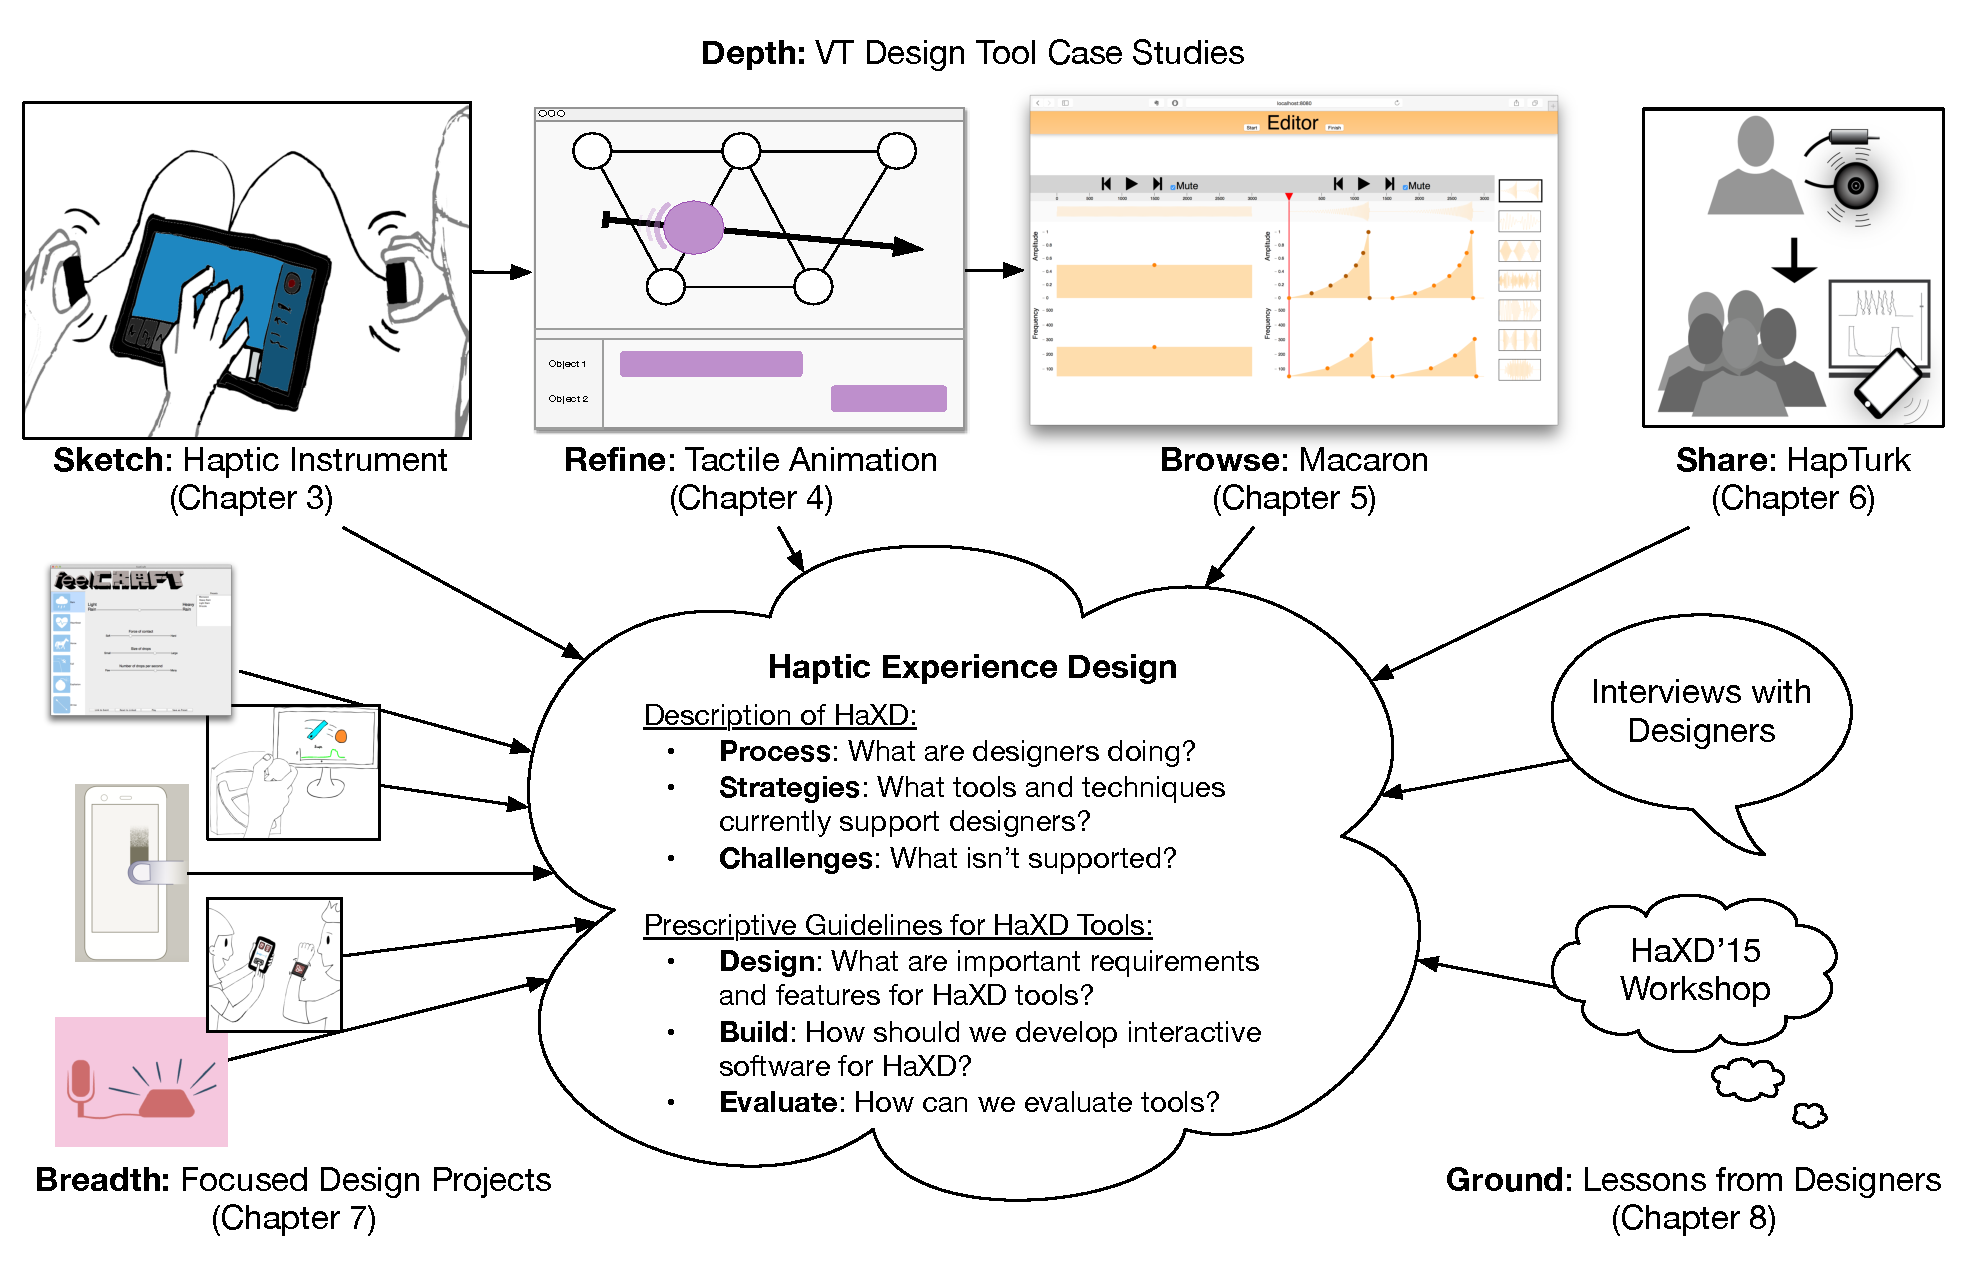
\includegraphics[width=\textwidth]{HaXDTheoryOutline-2016-08-11}
\caption{Approach overview. We investigate VT design tools (Chapters \ref{ch:hapticinstrument}-\ref{ch:macaron}) and techniques (Chapter \ref{ch:hapturk}) in-depth. These findings are synthesized with multiple, smaller focused projects (Chapter \ref{ch:applications}) and grounded data from hapticians (Chapter \ref{ch:hapticianinterviews}) into a preliminary understanding of \haxd.}
\label{fig:intro:methodologyoverview}
\end{center}
\end{figure}



\section{Approach}
While many tools exist to support design in other modalities, such as graphic design, there are few for haptics.
%Part of this comes from immaturity of the field and lack of market penetration of highly expressive haptic devices.
%However, there are also intrinsic challenges to designing for the sense of touch.
%I want to develop practical tools that support the HaXD process, building a body of knowledge of how to facillitate this difficult subfield of design.
We approach this problem with three strategies:
\begin{enumerate}
\item \textbf{Depth: Vibrotactile design tool case studies (Chapters \ref{ch:hapticinstrument}-\ref{ch:hapturk}).}
To understand design, I take a design perspective.
In each of three case studies, I design, build, and evaluate a tool or technique to support an aspect of \haxd, scoped to \emph{vibrotactile} (VT) design.
Each of these results in concrete implications for designing tools and a small window onto the larger HaXD process.
Contributions include algorithms, data structures, interaction techniques, features, analytic techniques, and working software tools that have been employed by designers.
\autoref{ch:hapticinstrument}, \autoref{ch:tactileanimation}, and \autoref{ch:macaron} outline iterative development and evaluation of VT design tools; \autoref{ch:hapturk} covers a VT design technique (proxies).

\item \textbf{Breadth: Focused haptic design projects (Chapter \ref{ch:applications}).}
While the case studies provide an in-depth investigation into VT sensation design, results may not generalize to other devices, and provide limited investigation into application areas like education.
To generalize from VT effects, explore other aspects of haptic design, and gain personal experience as a haptic experience designer, we participate in several smaller focused design projects, which lend a broader context to our findings.
\autoref{ch:applications} discusses these projects.

\item \textbf{Ground: Data from haptic experience designers (Chapter \ref{ch:hapticianinterviews}).}
Finally, despite the recent growth of the field, haptic designers remain relatively rare and difficult to recruit.
To complement our primarily design-based approach and ground it with haptic experience designers in the field, we draw from other data sources: a workshop held at World Haptics 2015 and interviews with haptic designers.
\autoref{ch:hapticianinterviews} discusses this characterization of haptic experience design.
\end{enumerate}


\begin{figure}[htbp]
\begin{center}
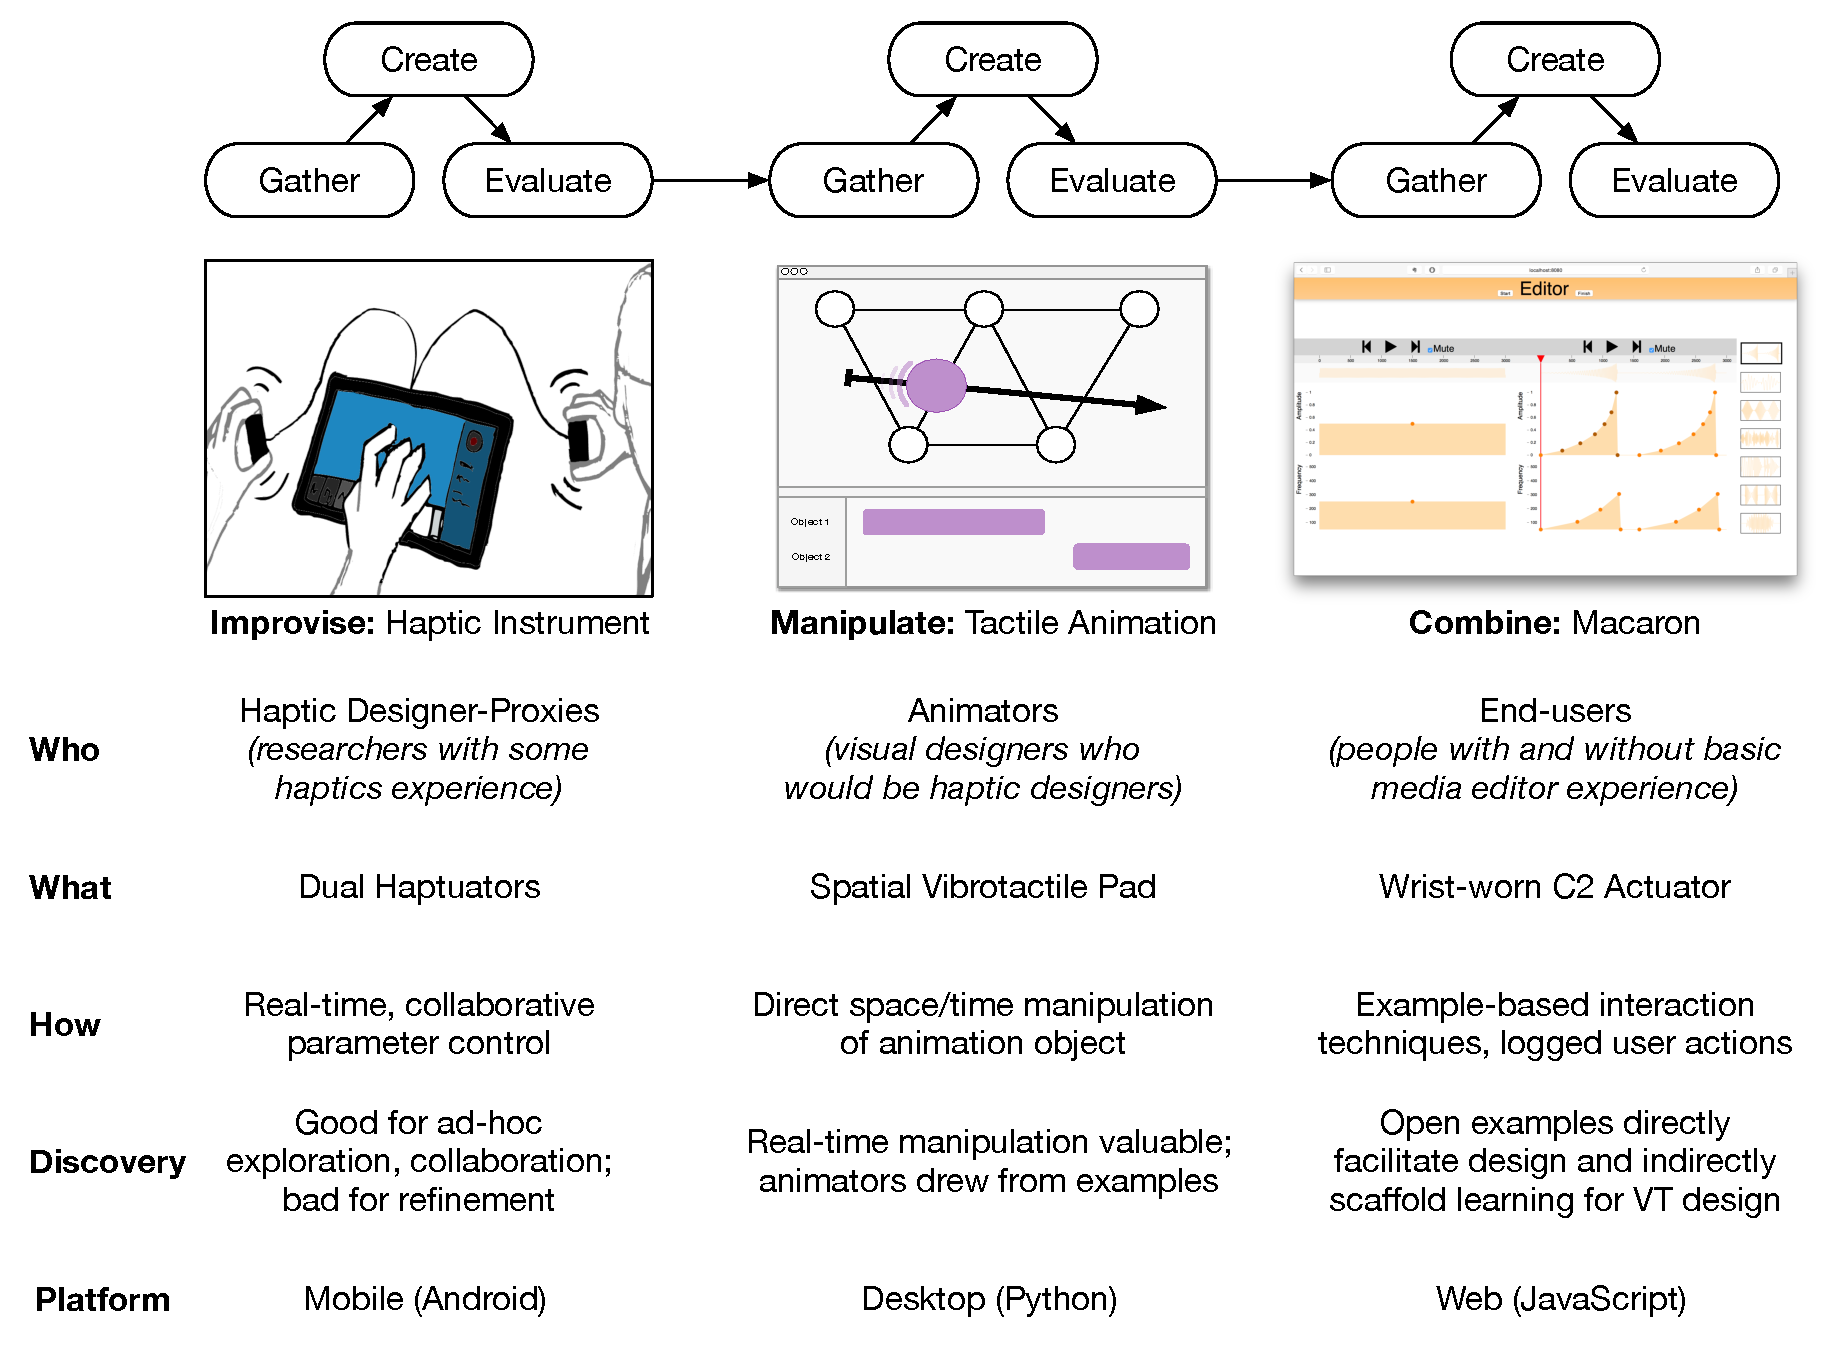
\includegraphics[width=\textwidth]{HaXDTheoryCaseStudyOutline-2016-08-11}
\caption{Vibrotactile design case studies. Each studies an aspect of vibrotactile design with a varied set of users, devices, platforms, and foci.}
\label{fig:intro:casestudyoverview}
\end{center}
\end{figure}



\subsection{Depth: Vibrotactile Design Tool Case Studies}

Each case study investigates a different set of design concepts with varying user populations, VT device, and design challenges.
We iteratively develop three \haxd support tools (\autoref{fig:intro:casestudyoverview}), but restricts scope to VT sensations.
This offers a deep look into an expressive and increasingly common class of haptic devices, allowing us to explore critical features in a somewhat controlled fashion.
An iterative approach allows us to refine ideas and methods, and so each case study follows three steps: \emph{gather}, finding requirements and previous design elements; \emph{create}, where we design and build the tool; and \emph{evaluate}, where we test the tool with its target population and consolidate lessons learned.
We also include a collaborative study for a VT design technique (``HapTurk").


\begin{description}

\item[Initial Exploration: The Haptic Instrument (\autoref{ch:hapticinstrument})]
In Study 1, the Haptic Instrument, we focus on real-time, rapid design of VT sensations with a first look into themes of real-time design and collaboration.
When participants worked with our tool, mHIVE (a ``mobile Haptic Instrument for Vibrotactile Exploration"), compositions couldn't be edited, suggesting mHIVE was suitable for exploration and improvised communication, but not as suited to refining ideas.
We also found informal, collocated collaboration useful, but leave future examination of collaboration support to side projects (described next in \autoref{ch:intro:approach:breadth}).

\item[Direct Manipulation Pipeline: Tactile Animation (\autoref{ch:tactileanimation})]
In Study 2, Tactile Animation, we developed a single abstracted animation object directly manipulated in both space and time.
In this study, we focused on building a usable tool to support exploration and refinement, and investigate a generalized rendering pipeline in detail to understand how to build haptic design tools.
Animators found our tactile animation tool, Mango, easy-to-use, and confirmed our findings about the value of real-time exploration.
We also found that ``soft features", like copy/paste and undo/redo, were extremely important.

\item[Example Use and Analytics: Macaron (\autoref{ch:macaron})]
One stand-out result from both Mango and mHIVE is that designers drew from their experience or examples found in the world, and wanted to re-use what they had created (e.g., through copy and paste).
In Study 3, we explore the role of examples in haptic design with a web-based tool, ``Macaron", a vibrotactile track-based editor with visible, incorporable examples directly embedded in the interface.
Macaron was implemented using the understanding we gained from Study 2, giving us more opportunity to focus on capturing and studying the design process, especially using interaction logs to investigate example use.
%This study is codenamed ``Project Macaron" and consists of two phases.
%Phase I, ``algorithms and interaction techniques", builds a set of perceptually-verified ways to manipulate examples and incorporate them into designs.
%In Phase II, we use the results of Phase I to create a haptic design gallery interface, and study how and when users incorporate examples into their VT designs.
%In this way we hope to consolidate our findings from mHIVE and Mango, and capture our participants' design process more concretely through logging of user actions.
We found examples were used primarily as templates to inform initial design, making each individual design easier but also scaffolding the user's understanding of how to create VT effects.
%These studies are described in more detail in \autoref{ch:hapticinstrument},  \autoref{ch:tactileanimation}, and \autoref{ch:macaron}.

	\item[Feedback at Scale: HapTurk (\autoref{ch:hapturk})]
	%is a collaboration with PhD candidate Hasti Seifi on different techniques to crowdsource feedback on VT icons. Master's student Salma Kashani and undergraduate Matthew Chun are developing visualizations and low-fidelity VT icons during summer 2015.
	While not an iterative design tool study, HapTurk is a focused investigation of a VT design technique for collecting large-scale feedback on VT icons.
	Haptic devices cannot be sent to hundreds or thousands of people for feedback, but collecting in-lab feedback can be expensive, and informal feedback from colleagues is limited in scope.
	We investigate whether visual or low-fidelity \emph{proxies} can stand in for high-fidelity VT effects, with implications for both collecting feedback and broadcasting VT sensations more widely.

\end{description}




\subsection{Breadth: Focused Haptic Design Projects}
\label{ch:intro:approach:breadth}
Each case study provides concrete knowledge for building a VT authoring tool, and some insight into the VT design process.
However, VT technology can be used in many different scenarios, and there are many devices and experiences that involve other haptic modalities.
To broaden our understanding of haptic design, we undertook several more focused haptic design projects to look at different activities, application areas, and haptic modalities.
In \textbf{\autoref{ch:applications}}, we describe several smaller projects that gave opportunities for practicing haptic design and exploring other types of haptic feedback:

\begin{description}
	\item[FeelCraft (\autoref{sec:applications:feelcraft})] is a plug-in architecture that augments media with customizable spatial VT effects.
	We use FeelCraft to explore existing infrastructure for haptic media, and to design VT effects for a popular video game, MineCraft.
	
	\item[Feel Messenger (\autoref{sec:applications:feelmessenger})] is a chat program augmented with expressive, customizable VT effects using commodity hardware and APIs.
	
	\item[RoughSketch (\autoref{sec:applications:roughsketch})] is a painting application for the TPad Phone, a variable-friction mobile device, for the World Haptics 2015 Student Innovation Challenge. 
	Variable friction is a significant contrast to VT sensations as it is intrinsically connected to input: no sensation can be felt without active movement by the user.
	
	\item[HandsOn (\autoref{sec:applications:handson})] is a conceptual model for creative education software using low-cost, DIY haptic hardware, giving us an understanding of how to work with 1-degree of freedom force feedback and an educational context.

	\item[CuddleBit (\autoref{sec:applications:cuddlebit})] is a project inspired by the Haptic Creature \cite{Yohanan2011affectivetouch,Yohanan2011affectdisplay,Chang2010} and CuddleBot project \cite{Allen2015cuddlebot}.
	We use small, breathing robots to explore the display of emotion, and extend our findings from VT design tools into new tools for this modality: Voodle and MacaronBit.

\end{description}





\subsection{Ground: Data from Haptic Experience Designers}
%In addition, it is difficult to find and recruit haptic designers.
\osC{TODO: Update this once I've gone over Ch8 again}
I will synthesize findings from the three design case studies together with a number of side projects, the design literature, community feedback from a workshop on haptic experience design, and interviews with haptic designers into a preliminary design theory on how to support the creation of engaging, captivating haptic experiences.
I expect to make progress on the following questions:


\begin{description}
    \item[Description of the Haptic Design Process.]
    What are the major \textbf{processes and tasks} conducted by haptic designers?
    What \textbf{strategies} do haptic designers employ, including existing tools?
    What are the \textbf{challenges} haptic designers face?
    
    
    \item[Prescriptive Implications for HaXD Tools.]
    What are major \textbf{requirements} and \textbf{features} for designing HaXD tools?
    What are some considerations when \textbf{implementing} HaXD tools in software?
    How can we \textbf{evaluate} design tools effectively?
\end{description}


\section{Outline and Contributions}
\osC{I've already outlined what I'm talking about. What else can I put here to set up the dissertation?}
\osC{TODO: unite this text with some of the previous descriptions, somehow.}
This dissertation continues as follows.
First, in \autoref{ch:rw}, I cover related work with an overview of haptic technology and applications, a presentation of existing haptic design tools, and a discussion of design theory from other fields.

Then, I outline each VT design tool case study in \autoref{ch:hapticinstrument},  \autoref{ch:tactileanimation}, and \autoref{ch:macaron}.
In \autoref{ch:hapticinstrument}, we present findings from our first vibrotactile design tool, the haptic instrument, which supported easy exploration and informal feedback, but identified a key problem: lack of refinement for designs.
In \autoref{ch:tactileanimation}, we present findings from our second vibrotactile design tool, Mango, which established a generalized pipeline and was able to support both exploration and refinement for expert visual animators; it highlighted reuse as an important next step.
In \autoref{ch:macaron}, we present findings from our third vibrotactile design tool, Macaron, which implemented a browsing interface and analytics system; we found examples played a large part of the design process, and that a web-based tool allowed for easy deployment.

%Each chapter is presented as a direct outline of what will appear in the final dissertation, summarizing either methods and results (\autoref{ch:hapticinstrument} and \autoref{ch:hapticanimation}) or proposed methods and possible results (\autoref{ch:hapticexamples}).
I then describe focused haptic design projects in \autoref{ch:hapturk} and \autoref{ch:applications}, and the results from our grounded data collection in \autoref{ch:hapticianinterviews}.\
In \autoref{ch:hapturk}, we document findings from HapTurk, a technique for getting feedback on vibrotactile designs at scale: from the crowd using proxy vibrations distributed over Mechanical Turk; we also comment on uses for haptic broadcasting.
In \autoref{ch:applications}, we synthesize together findings from our side projects, showing generality by applying our understanding of haptic design explicitly in several domains and gaining practical experience designing haptic experience.
In \autoref{ch:hapticianinterviews}, we complement our design-based inquiry through interviews with professional haptic designers and a workshop run to elicit feedback from the community; this captures a description of haptic design, reinforcing our findings for important support tools, and identifies more systematic challenges.

Finally, in \autoref{ch:conclusion}, we conclude with a summary of our final results and directions for future research.


%
% END
%
\endinput

Any text after an \endinput is ignored.
You could put scraps here or things in progress.


%    2. Main body
% Generally recommended to put each chapter into a separate file

%% The following is a directive for TeXShop to indicate the main file
%%!TEX root = diss.tex

\chapter{Background}
\label{ch:rw}

In this chapter, we provide the relevant background for this dissertation.
We begin with an overview of haptic technology and perception.
Next, we discuss the application space for haptics and why haptic experiences are increasingly important to design.
We then discuss the previous work in \haxd and related support tools, identifying why this is an area for improved understanding.
After, we discuss non-haptic creativity support tools and design theory which provided inspiration and guiding principles.
Finally, we present the qualitative and quantitative methodologies used in this dissertation.
Throughout the chapter, we contextualize this work and \haxd in both the haptics and HCI communities.


%%%%%%%%%%%%
%
% SECTION: What is haptics?
%
%%%%%%%%%%%%
\section{An Overview of Haptic Technology and Perception}
The term ``haptic" was coined by German researcher Max Dessoir to refer to the study of touch, in a similar to ``optic" for sight and ``acoustic" for sound \cite{Grunwald2008}.
Today, it refers to both the study of the psychology and perception of the senses of touch, and the technology that employs touch as a method of feedback.
Haptic technology is typically separated into two classes based on the main sense modality: \emph{tactile} sensations, and \emph{proprioception}, or the sense of body location and force;  the latter includes \emph{kinaesthetic} senses of force and motion.
These two types of feedback are useful for different purposes, \eg, people use their fingerpad's tactile senses to derive texture, but kinaesthetic feedback to infer weight \cite{Lederman1987};
different senses can be combined for more convincing results \cite{Okamura1998}.
An excellent overview of the haptic senses is available by \citet{Lederman2009survey}, and a practical introduction to the technology is available by \citet{Hayward2007}.
Here, we focus our coverage on the sensations directly studied by this dissertation, while also portraying the diversity of haptic experiences and technology.

\subsection{Tactile Perception and Technology}
%\osC{Goal: Explain the main mechanisms we use in the dissertation's studies, persuade the reader that I know enough about tactile perception, and show the variety of tactile displays and experiences.}
Tactile sensations rely on multiple sensory organs in the skin, each of which detect different properties, \eg, Merkel disks detect pressure or fine details, Meissner corpuscles detect fast, light sensations (flutter), Ruffini endings detect stretch, and Pacinian corpuscles detect vibration \cite{ChoiKuchenbecker2013}.
%Temperature and pain are also detected through \osC{todo}.
Of these, the Pacinian corpuscle is most widely targeted by technology through vibrotactile (VT) sensations, where vibrations stimulate the skin.
VT sensations are accessible, well-studied, and increasingly widespread, and can be passively felt, easing implementation.
Our in-depth design tool studies thus focus on VT experiences.

VT actuators can take may forms.
Eccentric mass motors (sometimes ``rumble motors" or ``pager motors") are found in many mobile devices and game controllers, and are affordable but inexpressive.
%An unbalanced mass is mounted on the motor, which provides dramatic shaking of the device.
More expressive mechanisms such as voice coils %  implemented in a variety of ways and 
offer independent control of two degrees of freedom, frequency and amplitude.
Piezo actuation is a very responsive technique that is typically more expensive than other vibrotactile technology.
% One of the more common and expressive is the C2 tactor, intended to directly stimulate the skin through contact or a thin membrane; the tactile animation project [] uses an array of C2 tactors.
While voice coils typically directly stimulate the skin, linear resonant actuators (LRAs) shake a mass back and forth to vibrate a handset in an expressive way; a common research example is the Haptuator \cite{Yao2010}.
Instead of directly stimulating the skin, this actuator typically shakes another device held by the user, such as a mobile device \cite{Yoo2014} or pen \cite{Culbertson2014}.
As of writing (2016), this type of actuator is increasingly deployed in consumer products (\eg, Apple's Taptic Engine).

%%%%In contrast to displacing the entire user body, recent multichannel haptic devices create percepts of dynamic and localized haptic sensations directly on the user's skin \cite{Israr2011} and in the mid-air \cite{Wilson2014}.
Actuators like VT devices can be used alone or put together spatial multiactuator displays like seats \cite{Israr2012,Israr2010}, belts \cite{Pielot2009,Paneels2013}, wristbands \cite{Arab2015,Paneels2013,Gupta2016}, vests \cite{Prasad2014,Jones2004}, and gloves \cite{Park2016,Kim2009}.
These can be arrange into grids, either dense tactile pixels (``taxels") \cite{Kim2009} or sparse arrays \cite{Israr2012,Israr2010}, to provide explicit 2D output on a plane.
Multiactuator arrays increasingly exploit tactile illusions to create effects of motion or phantom sensations in-between actuators.

Another emerging tactile feedback mechanism is programmable friction.
Surface friction, for example on a mobile touch screen, can be manipulated by both mechanical motion or electrical adhesion.
The TPad \cite{Winfield2007a} vibrates a plate at ultrasonic frequencies to create a cushion of air between the surface and the user's finger.
This effect is programmable, and can be used to with a number of interactive scenarios \cite{Levesque2011}.
Other techniques like electrovibration, deployed in TeslaTouch \cite{Bau2010}, and electrostatic forces \cite{Meyer2013} can create a similar effect.
Strong electroadhesion \cite{Shultz2015} has the potential to create even larger shear forces, but comes with a high power cost.
In RoughSketch (\autoref{ch:applications}), we design for a mobile version of the TPad deployed on Android devices, the TPad phone (\url{www.thetpadphone.com}).

There are many other types of tactile stimulation used in haptic experiences.
2-dimensional pin-based grids like Optacon \cite{Bliss1970} and HyperBraille (\url{www.hyperbraille.de}) can display Braille and 2D images to the blind and visually impaired, and operate as a generic computer display \cite{Prescher2010}. 
%"Survey on communication through touch" by pasquero, "Optical to tqactile image conversion for the blind by Bliss et all 1970.
Similar multi-point displays have been deployed on mobile devices.
Edge Haptics uses dozens of linearly-actuated pins on the edge of a mobile device for tactile stimulation, similar to a 2-dimensional braille pin display \cite{Jang2016}, while laterally moving pins can use skin-stretch as a display mechanism \cite{Luk2006}.
Electrocutaneous stimulation, where electrodes are directly activated on the skin, has been deployed for spatial tongue displays \cite{Bach-y-Rita1998}.
Temperature displays exploit warm and cold receptors in thea skin for display, using Peltier junctions \cite{Jones2002}.
Tactile sensations can be created at a distance using ultrasonic transducers \cite{Obrist2013,Carter2013} and vortex cannons that shoot puffs of air \cite{Sodhi2013}.



\subsection{Proprioception and Force Feedback}
%\osC{Goal: Explain the main mechanisms we use in the dissertation's studies, persuade the reader that I know enough about proprioception, and show the variety of force-feedback displays. This section will be smaller than the tactile section, and should make the distinction of verisimilitude and veridicality a bit clearer, because with FF we often have a virtual environment and are more concerned with passivity, stiffness, etc.}
Proprioception, the sense of force and position, is synthesized from multiple sensors as well: the muscle spindle (embedded in muscles), golgi-tendon organ (GTO) in tendons, and tactile and visual cues \cite{Kandel2000}.
We distinguish proprioception from the related term kinaesthetic by being the general, synthesized sense, where kinaesthetic sensation is strictly the sense of motion \osC{todo: make sure this is correct}.
Force displays are common in precise, specialized applications like robot-assisted surgery \cite{Okamura2009} or realistic sensorimotor training environments \cite{VanDerMeijden2009}.

Force-feedback devices might have degrees of freedom of feedback (DoF), the number of forces or torques they can display.
These devices render a \emph{virtual environment}, with simulated forces depending on the input from the user.
Common consumer-facing 3-DoF devices include the Geomagic Touch (previously the Sensable PHANTOM) and Falcon devices, offering force in three directions.
2-DoF designs like the pantograph \cite{Ramstein1994,Campion2005} can provide displays on screens, walls, and tables.
These displays have previously input on realistic simulation and rendering: \eg, making free space feel free, providing stiff virtual objects and walls, and avoiding saturation  \cite{massie1994phantom}.
Open-hardware, self-assembled versions of these devices, such as WoodenHaptics \cite{Forsslund2015} for 3-DoF devices and Haplet \cite{Gallacher2016} for 2-DoF displays, have the potential to make haptics more accessible.
Much previous work has been done on handling technical concerns, \eg, displaying complex polygonal objects with a ``God object" \cite{Zilles1995}, coordinating remotely situated devices or shared environments \cite{Buttolo1997}, and improving collision realism with transient forces \cite{Kuchenbecker2006}.
More complex environments are primarily programmed in using APIs like CHAI3D, OpenHaptics, or Unity.

Another approach is to use simple force feedback, especially for haptics education \cite{Jones2014}.
1-DoF devices include linear actuators pushing on the user and haptic knobs, \eg, the UBC Twiddler \cite{Shaver2003,Enriquez2003,MacLean2009a}, and paddles, \eg, the HapKit \cite{Martinez2016}.
The UBC SPIN lab has also adopted 1-DoF force feedback in its affective robot, the Haptic Creature \cite{Yohanan2011affectdisplay,Yohanan2011affectivetouch}, the CuddleBot, and CuddleBits \cite{cang2015cuddlebits}.
We explore force-feedback design with the HapKit and CuddleBits in \autoref{ch:applications}.


\subsection{Haptic Illusions}
Like visual displays' stroboscopic effect transforming a series of images into the perception of motion, illusions play a valuable role in haptic sensations \cite{Hayward2016}.
Some effects are influenced by other senses.
In the classic size-weight illusion \cite{charpentier1891analyse}, when two weights have the same mass but different sizes, the smaller is perceived to be heavier, whether size is seen or felt \cite{Hayward2016}.
A striking, recent example is the use of visual dominance to use a single physical block to provide haptic feedback for multiple virtual blocks by distorting the visual position of the user's arm \cite{Azmandian2016}.
We employ similar techniques in our FeelCraft and Feel Messenger projects, using visual feedback to prime users to haptic sensations (\autoref{ch:applications}).

Other illusions are purely tactile and useful for grid displays.
Phantom tactile sensations \cite{Alles1970}, create illusory vibrations in between two or more VT actuators, opening up the space in-between actuators for display.
Continuous motion can be simulated, \eg, \citet{Seo2010} created a perceived motion flow between two VT actuators mounted on the ends of a handheld device by controlling their intensity.
Similarly, \citet{Lee2012a} created across-the-body and out-of-the-body illusions on a mobile device using up to four % inexpensive 
linear resonant actuators; \citet{Gupta2016} used interpolation on a VT wristband for new interaction techniques.
The Tactile Brush algorithm \cite{Israr2011a} combined phantom tactile sensations and apparent tactile motion to render high-resolution and moving haptic patterns on the back using a coarse grid of VT actuators. 
Other spatio-temporal VT illusions such as the ``cutaneous rabbit"  \cite{Tan2009}, where carefully timed discrete tactile stimuli create perceived motion, and Tau and Kappa effects \cite{Hayward2008,Hayward2016}, where perceived distance between stimuli depending on their timing, can also be used with VT arrays.
Similar illusions are possible using other tactile modalities, including temperature displays \cite{Singhal2016} and electrocutaneous stimulation \cite{Tanie1980}.
We extend phantom sensations to 2D interpolation (\eg, between 3 actuators) to enable Tactile Animation (\autoref{ch:tactileanimation}).



\osC{Integrate this}
Of course, haptic perception can depend on the situation of the user, especially important in wearable contexts.
Vibrotactile detection depends on many variables, including location on the user's body, how much the user is moving, and whether they are expecting the vibration \cite{Karuei2011}, and social context \cite{Cauchard2016}.
These effects can be mitigated through sensing, \eg, detecting movement with accelerometers \cite{Blum2015}.




%\inlineHeading{Multimodal interaction}
%Similar to vision and audio, haptic perception is susceptible to illusions \cite{Hayward2016,Hayward2008}.
%
%discuss passiveness, like cobots, etc.

%%%%%%%%%%%%
%
% SECTION: Why should we care about haptics?
%
%%%%%%%%%%%%
\section{The Value of Haptic Experiences}
Haptic feedback can provide several benefits to interactive experiences.
Here, we outline the main benefits haptics provides, and then several application areas that commonly leverage those benefits.


\subsection{Why Touch?}
Haptic technology enables information transfer between humans and computers;
this transfer is rich, proximal, and fast.
Information flows both ways, through input and output, sometimes simultaneously.
We focus on designed haptic display.

One advantage of touch is simply that it is not vision or audio, the primary feedback methods for interactive systems.
Haptic technology can reinforce other modalities, enriching feedback for a more complete experience, or
provide complementary feedback, with many possible reasons:
information saturation, \eg, when visual or audio displays have maximized their output;
task context, \eg, when the user is driving and must keep their eyes on the road;
impairment or impairing situations, \eg, when a user has limited sight or hearing;
ambient displays, \eg, keeping a user aware of a piece of information without interrupting them;
or nature of the information, \eg, communicating emotion.
%It can increase general usability and provide an alternative path for information when other modalities are not available (\eg, the users are visually-impaired) or not appropriate (\eg, looking at a screen would be socially inappropriate).
Sensory substitution, first pioneered by Bach-y-Rita \cite{Bach-y-Rita1969}, is a dramatic technique often using haptic senses to augment or replace other senses.
A wide variety of devices have been developed and studied for the visually impaired (\eg, \cite{Prescher2010,Bliss1970}).

Of course, touch is a unique, rich sense in its own right.
Like sound, touch can be invisible; like vision, it can be spatial.
Feeling an object is especially helpful at discerning material properties \cite{Lederman1987}.
Touch is the first sense to develop, playing an important role in formative experiences \cite{Jansson-Boyd2011}.
Sensorimotor actions can help to scaffold understanding through embodied learning \cite{Papert1980}.
Touch can also be used for artistic expression; \citet{Gunther2002} studied a full-body vibrotactile suit to create music-like ``cutaneous grooves", helping to identify the artistic space of VT sensations, including concerts with tactile compositions.

While haptic feedback can improve usability and task performance \cite{Pielot2009,Chan2008}, touch is especially connected to visceral, emotional connections.
Marketing research has studied multiple ways that touch can connect with customers.
For example, the way a smartphone feels can influence a purchase over one that might work better, and customers prefer to shop at stores that let them touch products \cite{Spence2011,Jansson-Boyd2011}.

There are different models of models used in affective computing.
Two especially common models are Ekman's basic emotions and Russell's affect grid.
Ekman's basic emotions \cite{Ekman1992,Ekman1971} are a discrete set of emotions identified from a cross-cultural study of facial expressions; we use this model's emotions as the design task in \autoref{ch:hapticinstrument}.
Russell's affect grid \cite{Russell1989circumplexmodel,Russell1989affectgrid} separates emotions into dimensions of arousal (low to high energy) and valence (positive and negative emotions); this work informs much of our work on expressivity and especially the CuddleBit work in \autoref{sec:applications:cuddlebit}.

Researchers are starting to develop design guidelines to express emotions through haptic experiences.
Low-level parameters like amplitude, frequency, and duration have been linked to emotions: \citet{YongjaeYoo2015} showed that VT icons can express arousal and valence;
\citet{Obrist2015} established design parameters for mid-air ultrasound stimulation.
Because touch can be bidirectional, affective sensing can accompany haptic display.
Through the Haptic Creature project established a touch dictionary of gestures used to emotionally communicate with robots \cite{Yohanan2011affectivetouch}.
Touch-based surfaces can detect these gestures \cite{Flagg2013} through technologies like conductive fur and fabric \cite{Flagg2012}.






%emotion theory background
%Emotion can play different roles in technology, such as affective technology, hedonic qualities, or interactional dynamics \cite{Hook2008bodyemotion} \osC{need to dig deep to understand this}





%; see \citep{Hamilton-Fletcher2016} for a recent survey and discussion of user preferences.


%In many of these contexts, careful design is required.
% \citet{Arab2015}'s wrist based display worked best when using a metaphor-based approach \cite{Brunet2013a}, co-designing metaphors with their users.
% \citet{Cauchard2016} found rhythm-based pulses were more effective for portraying numbers in their in-situ study.




\subsection{Applications}
While realistic virtual environments for force-feedback haptic feedback is extremely helpful in medical or training applications \osC{todo}, we focus on applications that find increased value in an explicit design step.


\subsubsection{Immersive Media and Virtual/Augmented Reality}
A popular application for haptic experiences is augmented, immersive media experiences.
Actuated tactile feedback has been used as early as 1959 in the movie \emph{The Tingler}  \cite{IJsselsteijn2003}.
4D theatres and theme park rides use bursts of air or water sprays to engage the audience.
Companies like D-Box (\url{www.d-box.com}) augment films with haptic tracks that both low-frequency movements and high-frequency vibrations, and can be found in theatres across the world.
Buttkicker (\url{www.thebuttkicker.com}) also augments 4D theatres, and provides products for home theatre setups.

Haptic experiences are also increasingly of interest in virtual reality (VR) environments.
Skin stretch techniques, explored in \cite{Guinan2014} and now commercialized by Tactical Haptics (\url{tacticalhaptics.com}), augments virtual-reality setups by simulating forces and torques using handheld controllers, lending stronger immersion for virtual environments and VR games.
Haptic Turk \cite{Cheng2014} and TurkDeck \cite{Cheng2015} are innovative explorations of high-fidelity haptic experiences in virtual environments using people as actuators.
Impacto uses electrical muscle stimulation and a solenoid actuator to create wearable haptic feedback with both kinaesthetic and tactile feedback \cite{Lopes2015}.
Haptic retargeting distorts visual feedback to re-use a single physical block in a virtual block-building game \cite{Azmandian2016}.


Previous work has also attempted to add greater immersion to broadcast media by including haptic sensations.
\citet{Modhrain2001} present an early vision of Touch TV, using active touch with two-DOF actuators embedded in remote controllers; \citet{Gaw2006} follow up with editable position playback on a force-feedback device, played alongside movies or cartoons.
More recently, the proliferation of online streaming video has developed opportunities to add haptic sensations using novel data structures.
Tactile Movies \cite{Kim2009} looks into augmenting movies with spatial VT feedback, including an authoring interface.
\osC{todo} YouTube  \citet{Gao2013}
haptic-audiovisual (HAV) content \cite{Danieau2013} basics of composition \cite{Guillotel2016}


\subsubsection{Affective Computing}
We've discussed how touch is closely connected to emotion.
This has implications for design;
%emotional connection and relationship can influence preferred interaction models;
for example, couples are more comfortable with a ``hand stroke" metaphor for two remotely coupled haptic devices than strangers, who prefer a more less intimate ``ping-pong" metaphor \cite{Smith2007}.
Emotional display through touch has therapeutic applications.
\citet{Bonanni2006} created TapTap, a wearable that can record and playback VT equivalents of affectionate touch to support users in therapy.
Tactile displays target improved mental health \cite{Vaucelle2009} and aiding emotional understanding for autism \cite{Changeon2012}.
The Haptic Creature project explores affective touch in human-robot interaction (HRI) \cite{Yohanan2005,Yohanan2009,Yohanan2011affectivetouch,Yohanan2011affectdisplay};
this furry, zoomorphic robot can measurably relax users when they feel it breath \cite{Sefidgar2016}.





\subsubsection{Expressive Communication}
%interpersonal touch, and haptic interpretations of it
Touch is extremely important for interpersonal communication, from greeting a new acquaintance with firm handshake, to showing affection to a loved one; see \citet{Gallace2010} for an overview.
Of course, technologically can mediate touch between people, \eg, in remote collaboration or shared virtual environments \cite{Haans2006}.
\citet{Brave1997} introduced ``inTouch", mechanically linked rollers that enabled playful touch interactions at a distance.
ComTouch \cite{Chang2002a} used pressure input to send vibrations with between mobile phones, finding it was used for attention, turn-taking, and emphasis.
\citet{Hoggan2012} elaborated these findings a one month-study found users sent ``Pressages" (pressure messages) both for greetings and to emphasize speech or emotional messages.
\citet{Chan2008} used VT icons to coordinate turn-taking in an online system, featuring an extensive design process to create and perceptually verify icons that present system state and requests with varying urgency.
%\citet{Brown2006multidimensionaltactons} used tactons displayed on a user's forearm \osC{this is actually kinda boring this study}





\subsubsection{Mobile Alerts}
Mobile contexts are rife with opportunities for haptic feedback.
Ambient tactile displays can provide awareness can provide awareness and alerts without distracting the user.
VT feedback is affordable, low-power, and can be added to watches and wrist-bands \cite{Brunet2013a,Arab2015}, belts, vests, and other wearables.
Tactons \cite{Brown2006} are a type of haptic icon \cite{MacLean2003} that provide VT feedback, commonly in mobile applications.
Rhythm opens up a large design space, letting users learn 84 different icons \cite{Ternes2008} and can be applied with even light, low-cost rumble motors.
A 28-day study showed that rhythmic VT icons do not disturb users in daily activities and can communicate ambient information \cite{Cauchard2016}.
\citet{Hemmert2008} explored a life-like metaphor of pulsing and breathing to provide alerts, but found care needed to be taken to not be annoying.
Multiple actuators can be combined in mobile handheld devices to provide differentiable spatial information, enriching the VT icon design space \cite{Yatani2009a}.
VT icons produced by phones can represent multiple levels of urgency and source of an alert (\eg, voice call, text message, or multimedia message) \cite{Brown2006mobilealerts}.


\subsubsection{Guidance}
Guidance is a typical application for VT feedback, which can be invisible, mobile, and accessed without using vision or sound.
%Guidance is a major applications, especially for specific populations like the visually impaired \cite{} or older adults \cite{Arab2015}.
Spatial guidance through haptic wearable display can improve navigation with multiple actuators across several form factors, including belts \cite{Pielot2009,Lindeman2005}, wrist-bands \cite{Arab2015}, and vests \cite{Prasad2014}; in each case, the vibrations inform the user where to go with spatial vibrations or metaphorical spatial icons.
Periodic vibrations can guide a user's walking speed without large attentional demands \cite{Karuei2014}.
Tactile illusions like saltation can provide directional information for guidance \cite{Tan1997}; larger back-based displays are effective for guiding both attention and direction, \eg, in automobiles \cite{Tan2003}.
\citet{Brewster2010} used VT icons to provide awareness of nearby friends and colleagues.
%Guidance Linderman2005 \cite{Prasad2014} \cite{Pielot2009}





\subsubsection{Education}
Haptic technology has the potential to improve educational resources, especially to those lacking resources.
Montessori methods have long espoused the value of physical learning aids, especially using physical \emph{manipulatives} \cite{Montessori1917}.
There is evidence to support these techniques: in a meta-analysis of 55 studies, \citet{Carbonneau2013} found that physical manipulations improve several learning outcomes, with influence by other instructional variables.
Studies of gestures have also found value in students ``being the graph" by physically acting out mathematical shapes, grounding abstract knowledge in embodied experience \cite{Gerofsky2010}.
These techniques have roots in constructivist learning, where learners use existing understandings as a \emph{transitionary object} to understand new concepts \cite{Papert1980}.

Haptic technology is well-positioned to support embodied learning, and there is early evidence for its efficacy.
Haptic feedback has been shown to improve temporal aspects when training motor skills \cite{Feygin2002}.
In a study for molecular chemistry education, \citet{Sato2008} found students had higher test scores when they interacted with their haptic learning interface; students reported engagement.
In \autoref{ch:applications} we describe results from an early learning interface for low-cost haptic displays \cite{Martinez2016}, showing that haptic technology can improve engagement and make lasting impressions.

%\cite{Hook2008bodyemotion} (?)

%Active learning and creativity in education??

%%%%LEARNING
%%%\osC{Education}
%%%Recognition of the value of a hands-on, embodied approach to learning dates to 1907, when
%%%Maria Montessori opened a school where she used \emph{manipulatives} to teach a wide array of concepts ranging from mathematics to reading, e.g., by introducing the alphabet through children tracing their finger along large, cut-out letters~\cite{montessori_advanced_1917}.
%%%Constructivist learning theories posit that well-designed manipulatives can assist understanding by grounding abstract concepts in concrete representations ~\cite{papert1980,piaget_science_1970},
%%%%Their use today is 
%%%and are an accepted core principle in early math and science education, confirmed empirically~\cite{carbonneau_meta-analysis_2013}. 
%%%
%%%More recently, digital technologies are radically altering learning environments.
%%%Massive Open Online Courses (MOOCs) expand access, games motivate, and with graphical simulations (e.g., PhET~\cite{wieman_phet:_2008}), students can interact with abstractions to develop their understanding.
%%%However, these experiences are disembodied. Indirect contact via keyboard, mouse and screen introduces a barrier of abstraction that undermines the connection and path to understanding. 
%%%% that the interaction aims to promote. 
%%%
%%%
%%%Haptic (touch-based) technology should bring %able to bring
%%% benefits of physicality and embodied learning~\cite{dourish_where_2004} to interactive virtual environments. 
%%%It adds a sensory channel as another route to understanding~\cite{calvert_crossmodal_1998}; when deployed appropriately, active exploration can improve understanding~\cite{martin_physically_2005} and memory~\cite{glenberg_activity_2004} of new concepts. 
%%%Haptic tools have already shown promising results in many specializations, demographics and age groups, both
%%%to enhance lesson fidelity 
%%%% (e.g., physics and medical simulations)  -- don't have room for citations!
%%%and to increase engagement and motivation through tangibility and interactivity; e.g., with devices like Geomagic Touch\footnote{Prev. Sensable Phantom \url{www.geomagic.com/en/products/phantom-omni/overview}}~\cite{williams_implementation_2004} and SPIDAR-G~\cite{sato_haptic_2008}.
%%%
%%%Unfortunately, %t
%%%%These 
%%%%Sadly, 
%%%existing approaches have %suffer from 
%%%both hardware and software limitations.
%%%Actuated learning tools introduce physical issues of cost, storage, and breakage;
%%%devices are  too bulky, complex, or expensive for schools or self-learners.
%%%For software, it is hard for users to construct and explore their own haptic environments. Typically, users load a virtual system to interact with it haptically. This sidelines the rich learning potential of involving users with model construction~\cite{papert1980}.
%%%We address hardware with the HapKit~\cite{martinez_2016}, a \$50, simple, low-fidelity device constructed from 3d printed materials.  
%%%
%%%Our focus here is on software, with a new learning environment that lets users both construct and explore haptic systems. Until now, the only way for a user to construct a haptic system was by programming it herself. Our approach, inspired by Logo ~\cite{papert1980} and Scratch ~\cite{maloney2010}, is to ultimately % KM notes: currently we don't provide much power compared to programming. But it's planned for.
%%%provide much of the power of a programming language while hiding distracting complexity. 
%%%



%%%%%%%%%%%%
%
% SECTION: Why should we care about haptic experience design tools? What is the precise problem this dissertation is solving?
%
%%%%%%%%%%%%
\section{Previous Efforts for Haptic Experience Design}


\osC{just moved this from applications}
The Haptic Application Meta Language (HAML) \cite{Eid2006} is an XML-based data format for adding haptics to MPEG-7 video, eventually augmented with the HAML Authoring Tool (HAMLAT) \cite{,Ferre2008}.
\citet{AbdurRahman2010} eventually adapted an XML approach to YouTube, and \citet{Gao2013} developed related online MPEG-V haptic editing.
Augmented media experiences and HAV content \cite{Danieau2013},  have used different methods of input.
One approach is to use camera motion sourced from accelerometers \cite{Danieau2012} to actuate audience members' hands and head in a HapSeat \cite{Danieau2013a,Danieau2012a}.
Later editable with H-Studio \cite{Danieau2013c}, this work has proposed the concept of Haptic Cinemotography \cite{Danieau2014}, including basic principles of composition when combined with video \cite{Guillotel2016}.
Other approaches include automatic conversion of audio content
Several studies have looked into automatic conversion from audio streams \cite{Lee2013,Chang2005,Hwang2014} or video streams \cite{Kim2014} to VT or force-feedback output.


\subsection{Editors and design tools}
As long as designers have considered haptic effects for entertainment media, they have needed compositional tools % to facilitate their design 
\cite{Gunther2002}.

Custom editors (such as D-Box Motion Code Editor) and software plugins are provided to media designers that overlaid the visual and audio content with haptics, and allow designers to generate, tune and save frame-by-frame haptic content in an allocated track for it to play simultaneously with the media content. 

By tuning parameters of these effects, users could personalize  haptic content, embed it in games and share effects with other users.
Similar devices and authoring schemes are also developed for online social interactions using custom multi-actuator haptic devices \cite{Kim2009,Tsetserukou2009,Paneels2013}.%Tsetserukou, D. and Neviarouskaya, A. iFeel_IM!: augmenting emotions during online communication. Comp. Graphics & Applications 30 (2009), IEEE, 72-80.
A great deal of previous work has focused on how to prototype or author haptic phenomena using non-programming methods. 

Many user-friendly interfaces help designers create % control 
haptic sensations, especially with vibrotactile devices.
The Hapticon editor \cite{Enriquez2003}, Haptic Icon Prototyper \cite{Swindells2006}, and posVibEditor \cite{Ryu2008} use graphical mathematical representations to edit either waveforms or profiles of dynamic parameters (torque, frequency) over time.
The Vibrotactile Score \cite{Lee2009} was shown to be generally preferable to programming in C and XML, but required familiarity with musical notation \cite{Lee2012}. 
%Mobile tools make haptic design more accessible.
The Demonstration-Based Editor \cite{Hong2013} allows control of frequency and intensity by moving graphical objects on a touchscreen.
%mHIVE, a Haptic Instrument \cite{Schneider2014} controls frequency, intensity, waveform and amplitude envelope of two tactors with touchscreen gestures.
Similar to the SPIN lab's Haptic Instrument (mHIVE, \autoref{ch:hapticinstrument}), this mobile tool was shown to be intuitive and easy to use for exploration or communication, but faltered when refining more elaborate sensations. %for a set context.

Commercially, Apple's end-user vibration editor has been present in iOS since 2011 (iOS 5) but only produces binary on/off timing information.
Immersion provides two tools: TouchSense Engage is a software solution for developers, while Touch Effects Studio lets users enhance a video from a  library of tactile icons supplied on a mobile platform.
Vivitouch Studio allows for haptic prototyping of different effects alongside video (screen captures from video games) and audio, and supports features like A/B testing \cite{Swindells2014}.
%More recently, Vivitouch Studio \cite{Swindells2014} allows for haptic prototyping of different effects alongside video (screen captures from video games) and audio, including features like A/B testing for simultaneous comparison of haptic content and exporting of a haptic video channel.


The control of multi-actuator outputs has been explored by TactiPEd \cite{Paneels2013}, Cuartielles' proposed editor \cite{Cuartielles2012}, and the tactile movie editor \cite{Kim2009}; the latter combined spatial and temporal control using a tactile video metaphor for dense, regular arrays of tactile pixels (``taxels"), including a feature of sketching a path on video frames. 
However, these approaches embrace the separate control of different actuators, rather than a single perceived sensation produced by the multi-actuator device, which we address with tactile illusions in \autoref{ch:hapticanimation}.

%The hapticon editor \cite{Enriquez2003}, haptic icon prototyper \cite{Swindells2006}, posVibEditor \cite{Ryu2008}, and Immersion's Haptic Studio (www.immersion.com) use a graphical representation to edit either waveforms or profiles of dynamic parameters (such as, torque) over time.

%Both emphasize exploration and broad manipulation rather than finely controlled end results.


\subsection{Platforms?}

There are many software libraries aim to support developers.
The UPenn Texture Toolkit contains 100 texture models created from recorded data, rendered through VT actuators and impedance-type force feedback devices \cite{Culbertson2014}.
The HapticTouch Toolkit \cite{Ledo2012} and Feel Effect library \cite{Israr2014} control sensations using semantic parameters, like ``softness" or ``heartbeat intensity" respectively.
%and Feel Effects  provide examples for vibrotactile actuators, like those found in game controllers and mobile devices.
Vibrotactile libraries like Immersion's Haptic SDK (immersion.com) connect to mobile applications, augmenting Android's native vibration library.
%FeelCraft's plugin architecture connects feel effects to various media types \cite{SchneiderAsiaHaptics2014}.
Force feedback devices have software platforms like CHAI3D (chai3d.org), H3D (h3dapi.org), and OpenHaptics (geomagic.com). 

Hardware prototyping platforms like
Arduino (arduino.cc) provide an open source microcontroller % platform 
and development platform % environment
for physical prototyping.
Phidgets (phidgets.com) facilitate rapid hardware prototyping with over 20 programming languages 
\cite{Greenberg2001}.
More recently, Wooden Haptics gives open-source access to fast laser cutting techniques for force feedback development \cite{Forsslund2015}, and
% Projects like 
faBrickation streamlines prototyping for 3D printing \cite{Mueller2014}. % and other manufacturing techniques.
These platforms, especially Arduino, have made significant improvements to enable rapid iteration and hardware sketching.
However, I believe we can do much better: these platforms require programming, hardware, and haptics expertise, and include inherent time costs like compilation, uploading, and debugging.



\subsection{Language of touch \osC{and schema?}}
Some higher-level perspectives offer outcome targets or design attitudes to guide haptic practitioners.
``DIY Haptics'' categorize  feedback styles and design principles \cite{Hayward2007,MacLean2008}.
``Ambience'' is proposed as one target for a haptic experience \cite{MacLean2009}.
Haptic illusions can serve as concise ways to explore the sense of touch, explain concepts to novices and inspire interfaces \cite{Hayward2008}.
``Simple Haptics'', epitomized by \emph{haptic sketching}, emphasizes rapid, hands-on exploration of a creative space \cite{Moussette2010,Moussette2011}. % with a design perspective \cite{Moussette2010,Moussette2011}.
Haptic Cinematography \cite{Danieau2014} uses a film-making lens, discussing physical effects using cinematographic concepts.
The notion of distributed cognition \cite{Hutchins1995} has particular relevance for haptic design, % provides an important perspective for haptic design in particular, 
suggesting that people situate their thinking both in their bodies and in the environment.
Haptics courses are taught with a variety of foci including perception, control, and design, providing students with an initial repertoire of skills \cite{Okamura2012, Jones2014}.

Haptics has often made use of metaphors from other fields.
Haptic icons  \cite{MacLean2003}, tactons \cite{Brewster2004}, and haptic phonemes \cite{Enriquez2006} are small, compositional, iconic representations of haptic ideas.
Touch TV \cite{Modhrain2001},  tactile movies \cite{Kim2009}, haptic broadcasting \cite{Cha2009}, and Feel Effects \cite{Israr2014} attempt to add haptics to existing media types, especially video.

Musical analogies have frequently been used to inspire haptic design tools, especially VT sensations. %unique.
The Vibrotactile Score, a graphical editing tool representing vibration patterns as musical notes, is a major example \cite{Lee2012, Lee2009}.
%The vibrotactile score provides an abstraction beyond low-level parameters and can draw from a musician's familiarity with the notation.
Other musical metaphors include the use of rhythm, often represented by musical notes and rests \cite{Ternes2008,Brown2005,Chan2008, Brown2006a}.
Earcons and tactons are represented with musical notes \cite{Brewster1993,Brewster2004}, complete with
tactile analogues of crescendos and sforzandos \cite{Brown2006}.
The concept of a VT concert found relevant tactile analogues to musical pitch, rhythm, and timbre for artistic purposes \cite{Gunther2002}.
Correspondingly, tactile dimensions have been also been used to describe musical ideas \cite{Eitan2010}.


%\subsection{Language of Tactile Stimuli}
The language of tactile perception, especially affective (emotional) terms, is another way of framing haptic design.
%The language of tactile stimuli has a long history in psychological studies \cite{Okamoto2013}.
Many psychophysical studies have been conducted to determine the main tactile dimensions with both synthetic haptics and real-world materials  \cite{Enriquez2003,Okamoto2013}.
Language is a promising way of capturing user experience \cite{Obrist2013}, and can reveal useful parameters, e.g., how pressure influences affect \cite{Zheng2012}.
Tools for customization by end-users, rather than expert designers, are another way to understand perceptual dimensions \cite{Seifi2014, Seifi2015}.
However, this work is far from complete; touch is difficult to describe, and some even question the existence of a tactile language \cite{Jansson-Boyd2011}.
%There is a clear need to empirically investigate the subjective experience of touch-based interfaces, for which phenomenology is ideal \cite{Creswell2013, Moustakas1994}.
%Start with hapticons, tactons, vibrotactile icons, Earcons, Auditory icons...
%Participants described two different sensations, one oscillating at 16 Hz and the other at 250 Hz.



%%%%%%%%%%%%
%
% SECTION: What other inspirations can we draw from? How are we approaching the above-mentioned problem? What scope is reasonable.
%
%%%%%%%%%%%%
\section{Non-Haptic Design and Creativity Tools}

%%%\section{Non-Haptic Design Theory}
In this section, we present related work on non-haptic design organized into three major elements: problem preparation, hands-on design, and collaboration.

\subsection{Problem Preparation}
Creative tasks, like design, are often defined as the recombination of existing ideas, with a twist of novelty or spark of innovation by the individual creator \cite{Warr2005}.
Also known as the ``problem setting" \cite{Schon1982}, ``analysis of problem" \cite{Warr2005}, or ``collect" \cite{Shneiderman2000} step, problem preparation involves getting a handle on the problem,  drawing inspiration from previous work. %, and and establishing a first general approach with which to attempt a solution.
Sch\"{o}n demonstrated that designers initially frame their problems before developing a solution \cite{Schon1982}.
Sch\"{o}n also describes the designer's repertoire, their collected experience, which aids in design.
External examples are especially useful for inspiration and aiding initial design \cite{Herring2009,Buxton2007}, which we explore in \autoref{ch:hapticexamples}.


%%Framing, finding the appropriate metaphor for thinking about the problem \cite{Schon1982}.
%When encountering a new problem, a designer begins \emph{framing}, finding the appropriate metaphor for thinking about the problem, typically drawn from her experience.
%In this way, metaphors that people already understand can be used to learn about new situations as a transitionary object \cite{Papert1980}.
%%Framing involves transforming the problem so that the designer can get a handle on it and begin to make progress.
%\emph{Framing} could involve a set of constraints upon the design problem, a list of requirements, or notational language to describe the problem.
%The more we can say about the problem, the more we can make progress on the solution.
%
%When \emph{framing}, designers draw from a \emph{repertoire} of their own previous experience that guides their design, storing cases, images, understandings, and actions \cite{Schon1982}.
%This approach is widespread in the haptics literature (e.g., ``haptic icons"  \cite{MacLean2003}, ``touch TV" \cite{Modhrain2001}), suggesting that we often have to rely on outside metaphors to describe concepts in haptics.
%
%Designers draw both from their \emph{repertoire} and from others' design \emph{examples}.
%While other sources sometimes use ``example" to refer to previously-encountered case studies \cite{Schon1982}, we consider those as part of the \emph{repertoire} and use ``example" exclusively to refer to externalized resources.
%In other fields of design, designers clip, store, and display \emph{examples} for inspiration \cite{Buxton2007} (\autoref{fig:corkboard}).
%Industrial designers collect various knobs and materials, and web designers bookmark sites \cite{Herring2009}.
%Managing these \emph{examples} effectively is already a significant task even in these more visual fields.
%%; with haptics, which often involves both software and hardware, this becomes a serious barrier.
%To work effectively with \emph{examples}, we need to have ways to capture, visualize, and recall them \cite{Herring2009}.

\subsection{Hands-On Design}
There has recently been a shift in how we interpret the act of thinking.
No longer is thinking relegated to the head; cognition is now seen as being situated in the physical world \cite{Hutchins1995}.
The designer must iteratively generate a varied set of initial ideas  (ideation) and then prune them (evaluation), repeating this step many times to settle on a single design \cite{Buxton2007}.
Working with multiple ideas simultaneously is a boon to good design.
Developing interfaces in parallel can facilitate generation and evaluation, delaying commitment to a single design \cite{Hartmann2008, Resnick2008}, while
in groups, sharing multiple designs improves variety and quality of designs \cite{Dow2011}.


Sketching supports ideation, evaluation, and multiple ideas,
allowing the designer to
explicitly make moves in a game-like conversation with the problem \cite{Schon1982}.
It is so important that some researchers declare it to be the fundamental language of design, like mathematics is the language for scientific thinking \cite{Cross2006}.
The power of sketching, according to Cross, is contained in its ability to describe a partial model of a proposed design or problem.
Detail can be subordinated, allowing a designer to zoom-in, solve a problem, and then
abstract it away when returning to a high-level view.
%\osC{cut this paragraph - should some of it be incorporated?}
This has implications for software tools: designers must easily navigate the design space with undo, copy and paste, and a history of progress, creating tools with a ``high ceiling" and ``wide walls" \cite{Resnick2008}.


\subsection{Collaboration}
Design is a collaborative process with the potential for generating more varied ideas \cite{Warr2005}, and is important for creativity support tools \cite{Resnick2008,Shneiderman2000}.
Although sometimes group dynamics influence the design process negatively, proper group management and sharing of multiple ideas results in more creativity and better designs \cite{Herring2009}.
Shneiderman in particular has championed collaboration in design \cite{Shneiderman2000}, and suggests two different types of collaboration to be supported by creativity tools: \emph{relating}, informal discussions with colleagues, and \emph{donating}, disseminating information to the public/annals of time.
Orthogonal to these intended purposes (relating and donating) is the collaboration context.
Computer-supported collaborative work often separates interactions into four contexts ordered into two dimensions: collocated (same location) or distributed (different locations), and synchronous (simultaneous)  or asynchronous (at different times) \cite{Ellis1991}.
Collaboration is notable because it is inherently challenging to haptic design: two people can look at the same image or hear the same sound from across a room, but touch is a local sense, far easier in a collocated, synchronous setting.
We explore collaboration with the Haptic Instrument (\autoref{ch:hapticinstrument}) and the FeelCraft and HapTurk side-projects (described in \autoref{ch:haxd}).


% (\autoref{tab:groupware}).
%Considering these different contexts illuminates specific goals when supporting haptic experience design.

%\begin{figure}[tbp] %  figure placement: here, top, bottom, or page
%   \centering
%   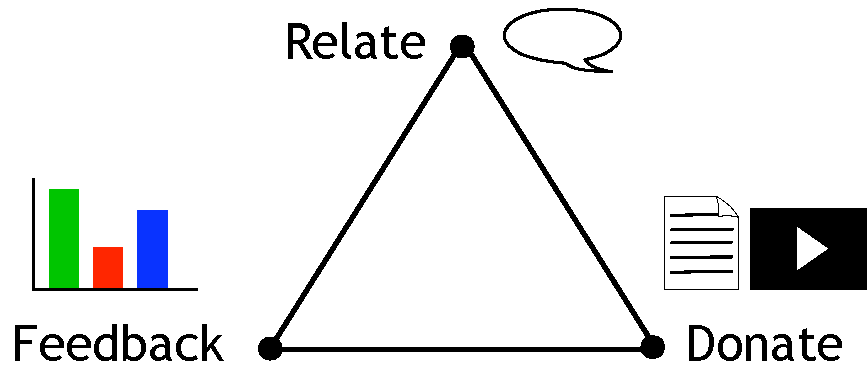
\includegraphics[width=0.33\textwidth]{figures/CollaborateSubProcesses2} 
%   \caption{Collaboration sub-activities. Designers work collaboratively in a continuum between \emph{donating}, \emph{relating}, and gathering \emph{feedback}.}
%   \label{fig:collaborate:sub:activities}
%\end{figure}

%\subsection{Challenge - Distributed Haptics}

%However, collaboration in the remote or asynchronous case is more challenging.
%Haptics has long been examined in remote collaboration both with force feedback \cite{Kim2004} and tactile \cite{Chan2008} mechanisms.
%Remote collaboration to support haptics, on the other hand, is a different beast.

%\subsubsection{Asynchronous collaboration}
%Collocated collaboration is common and well supported in haptics.
%In the synchronous case, \emph{relating} is a common activity, e.g., getting labmates and visitors to quickly try a prototype. User studies typically occur
%face-to-face as well, and 
%demonstrations at conferences \emph{donate} haptics to the community (indeed, the haptics community prioritizes demos so much that the inaugural Asia Haptics conference in 2014 was entirely in demo format).
%Asynchronous collaboration is less typical, with special advantages and issues.
%More investigation into asynchronous collaboration could reap rewards of self-running demos and user studies that collect copious data from diverse deployments % result in self-running demos and user studies that collect large amount of data from diverse populations (by deployment into different areas) 
%at low time cost to HaXD practitioners.
%%While more formal activities like feedback or donation could also be imagined , asynchronous collaboration is \kmC{get more specific : poorly understood}.
%%(self-running user studies or tactile installations \cite{Laaksolahti2011})

%\subsubsection{Distributed collaboration}
%Working remotely is even more challenging, both for synchronous and asynchronous contexts.
%Haptics involves physical devices and is a proximal sense.
%When working at a distance, there must be two identical devices.
%This means all components must be identical, whether electrical (e.g., amplifier settings), mechanical (e.g., joint dampening), or software.
%
%Distributed \textit{relating} can be supported in some small-scale cases.  % because of the small scale of devices.
%Each colleague could have a calibrated, identical device with synchronized software.
%% Because each colleague is expected to be 
%When each collaborator is knowledgeable about the device, video chat and email could provide sufficient support for many applications.
%Devices can be shipped or fabricated and calibrated at each location.
%While this introduces delay, slowing iteration and adding communication overhead, it is achievable.
%





%%%%%%%%%%%%
%
% SECTION: Methodology. How will we transform the above-mentioned approach into knowledge? How can we study our solutions?
%
%%%%%%%%%%%%
\section{Methodology}

Studying design process, creativity support tools, and haptic sensations is challenging and requires a robust methodology.
Our research questions seek to describe the process, strategies, and experience of \haxd, and to inform the design of supporting tools.
%As we have seen in our discussion of creativity and design support, systems of creativity tools are complex and noisy.
Our approach is to use mixed methods, as appropriate for our research questions.
We begin by using qualitative techniques to gather rich, generative data from design tools and design processes, and to inform iteration.
Through our work, we increasingly complement this data with quantitative methods, moving towards large-scale data collection for our generated theories with deployed tools.
%Furthermore, this work is an early inquiry requiring inductive models of thinking to generate theories, and the flexibility to accommodate invention as part of the inquiry, \eg letting us build tools iteratively based on participant feedback.
%As such, we turn to qualitative methodologies first and foremost, and as we gather findings, we gradually apply more hypothesis-testing-based approaches in a quantitative tradition.


\subsection{Inspiration and Perspectives}

extended mind and embodiment
Distributed cognition, embodiment, extended mind...
??

\subsection{Qualitative methodologies}
In this dissertation, we draw from the philosophical and methodological traditions of phenomenology, and the methodology of grounded theory.

Phenomenology is both a philosophical tradition and a social science methodology based upon that tradition that involves the study of subjective experience.
We use \citet{Moustakas1994} as our primary guide through both, as it focuses on practical methodological concerns but provides a strong philosophical background; \citet{Creswell2013} provided an overview of various methodologies and resources for phenomenology.
Critical components include \emph{horizonalization}, or preparing oneself to consider all of the participant's statements equally and with fresh eyes; distinguishing and synthesizing \emph{textural} descriptions, \eg the participant's verbatim explanation of the experience, with \emph{structural} description, or the analytical interpretation through psychology (or HCI) theories; and the documentation of the researcher's own experience with the phenomenon of study.
Phenomology as a methodology has been used in psychology to investigate topics ranging from visual illusions to tactile experience \cite{Richer1978, Obrist2013, Creswell2013}.

Methodologies, like phenomenology, often include a set of methods combined with their philosophical and epistemological underpinnings.
In this work, we specifically use the Stevick-Colaizzi-Keen methods as described by \citet{Moustakas1994}.
Transcripts are divided into non-overlapping, non-redundant statements about the phenomena known as Meaning Units (MUs).
This considers every statement that the participants make, and does not discount any due to bias or selective searching.
Then, MUs are clustered into emergent themes through affinity diagrams, writing and re-writing of thematic descriptions, and reflection guided by phenomenological philosophy.
We use this technique exactly in our first exploratory study (\autoref{ch:hapticinstrument}), and later combine it with Grounded Theory methods.

Grounded Theory is another well-known methodology first described by \citet{glaser1966awareness}.
We adopt the more flexible methodology described by \citet{Corbin2008}, as it allowed us to integrate with our phenomenological methods.
We principally adapt the methods used in Grounded Theory, specifically, memoing (writing about each focused quotation or MU), constant comparison (comparing each new memo and codes to previous ones), and open and axial coding (creating codes, or concepts, linking them together, then categorizing statements or observations based on codes).
This technique especially facillitated video analysis in \autoref{ch:tactileanimation} and \autoref{ch:macaron}, and allowed for quantitative count-based data and simple statistics to complement our interview-based findings.

We also note that researchers who use methods from the umbrella term ``qualitative research" often blend techniques from many methodologies.
Phenomenology and grounded theory are two such methodologies, others include hermeneutics, ethnography \cite{Moustakas1994}, ethnomethodology, and thematic analysis \cite{Ryan2003}.
For example, ethnography introduces the concept of ``thick description" \cite{}, where the research tries to use detailed, evocative language to convey a rich sense of being in the observed environment.
This technique is used more generally in observational notes and when writing up qualitative results to provide the rich data studied by qualitative methods.

\subsection{Towards quantitative methods at scale}
While some design scholars adopt qualitative techniques \cite{Schon1982,Cross2007,Cross2011}, others have developed quantitative techniques.
When studying graphic design for ads, \citet{Dow2011} used ratings by experts as well as click-through rates and other online analytics for actual deployed ads from their study.
\citet{Kulkarni2012} used MTurk to generate sketches of aliens in several conditions (of exposure to examples), then deployed another MTurk task to label each drawing with features like antennae or feet.
\citet{Lee2010a} had end-users rate graphic designs in both an in-lab study and over Mechanical Turk, and recorded time participant designers spent on each component.
These approaches allow for hypothesis testing for specific research questions, but require infrastructure unavailable to haptics, notably, crowd deployment, rating scales, and mature input tools.
In our early work, we found qualitative feedback to be sufficient while developing our understanding of how to build design tools.
Later, we begin to approach this infrastructure, using an online editor with analytic logs in Macaron (\autoref{ch:macaron}), and examining the potential for crowdsourced feedback with HapTurk (\autoref{ch:hapturk}).
While a valuable goal, large-scale quantitative feedback on \haxd remains outside the scope of this dissertation.



%%%%Unfortunately, these approaches do not scale to %\kmC{slc} % KM: seems like references to 'feedback' 'donate' etc should all be italicized because of their special sense.
%%%%formal \emph{feedback} or wide-spread \emph{donate tasks}, which typically have a large or anonymous audience with diverse % limited 
%%%%resources.
%%%%A wide-spread standardized device platform could support distribution, but given the variety of haptic effects \cite{Hayward2008}, this is extremely limiting and would tend to enforce a `lowest common denominator' effect.
%%%%Without assuming standardization, we suggest two possible solution strategies, each with tradeoffs:
%%%%accessible fabrication and device generalization.
%%%%
%%%%Fabrication methods like 3D printing are increasingly accessible. % to end-users.
%%%%%At a recent meeting with collaborators conducting 3D printing of haptic devices to a wide spread 
%%%%%\kmC{slc} % KM: following sentence confuses me, does it follow from 1st? Should there be a 'however"? Why does the complexity of haptic device manufacture fit it best for asynchronous collab - wouldn't that be better for synchro + collocated? 
%%%%However, manufacturing haptic devices is
%%%%complex, with software, moving parts,  and electronics, often requiring some assembly, best suited for asynchronous collaboration.
%%%%Furthermore, there is no guarantee that users have assembled their devices correctly.
%%%%Collaborators at a recent workshop found it difficult to verify % noted the difficulty in verifying 
%%%%system dynamics on their kit-based device in an asynchronous \textit{donate} task.
%%%%A resulting brainstorm \emph{ideated} a small calibration element to capture system dynamics, and a suite of diagnostic checks to help devices be consistent (e.g., template virtual environments with described ``correct behaviour").
%%%%%One promising area for investigation is in calibration tools to ensure remote devices are operating in similar fashion.
%%%%More advanced fabrication techniques may be able to improve this problem, producing moving parts, electronics, or other essential components.
%%%%
%%%%A second approach is to not attempt identical devices, but ensure they communicate what needs communicating.
%%%%We define device generalization in haptics as \emph{consistently reproducing intentional aspects of a haptic sensation}.
%%%%For example, a user watching a video of a force-feedback device on their phone could feel the force vector magnitude as vibration intensity (a \emph{donate} task), or a video chat could be augmented with a virtual environment rendered on force-feedback devices with different complexity.
%%%%This approach relies on partial standardization -- some sort of infrastructure is in place that facilitates constant output, for example, haptic broadcasting \cite{Cha2009}, touch TV \cite{Modhrain2001}, cinematography \cite{Danieau2014}, and tactile movies \cite{Kim2009}.
%%%%This is a challenging area, full of cross modal effects and contextual considerations (how is the user holding their phone?).
%%%%However, we think this is a promising approach while fabrication develops, especially for a \emph{donate} task in both synchronous and asynchronous interactions.
%%%
%%%
%%%
%%%
%%%\osC{SLC for HapTurk RW}
%%%%\section{Related Work}
%%%%We cover work related to VT icons and evaluation methods for VT effects, the current understanding of affective haptics, and work with Mechanical Turk in other modalities.
%%%%   %% \subsection{VT Icons}
%%%%     
%%%%		%%[change first sentence] VT effects are useful. According to previous studies, VT icons can communicate information [ref] and affect [ref]. VT effects are developed to assist visually-impaired users in outdoor scenarios [ref] as well as accessing digital information [ref]. In addition, VT effects can increase performance on visual interfaces, enhance engagement with the content and provide better user experience with electronic devices [ref to levesque].
%%%%		
%%%%\subsection{Existing Evaluation Methods for VT Effects} 
%%%%
%%%%The haptic community has appropriated or developed many types of user studies to evaluate VT effects and support VT design.
%%%%These target a variety of objectives:
%%%%
%%%%1) {\em Perceptibility:} Determine the perceptual threshold or Just Noticeable Difference (JND) of VT parameters. Researchers vary the values of a VT parameter (e.g., frequency)
%%%%% in small steps
%%%%to determine the minimum perceptible change
%%%%%for the parameter
%%%%~\cite{JNDstudy,foundationsoftactile}. 
%%%%
%%%%2) {\em Illusions:} Studies investigate effects like masking or apparent motion of VT sensations, useful to expand a haptic designer's palette \cite{Hayward2008,Israr2011a,Seo2013}.
%%%%
%%%%3) {\em Perceptual organization:} Reveal the underlying dimensionality of how humans perceive VT effects (which are generally different than the machine parameters used to generate the stimuli).
%%%%Multidimensional Scaling (MDS) studies are common, inviting participants compare or group vibrations based on perceived similarity~\cite{Hollins93,van2003distilling,Pasquero2006,Chan2008,Ternes2008}.
%%%%
%%%%4) {\em Encoding abstract information:} Researchers examine salient and memorable VT parameters (e.g. energy, rhythm) as well as the number of VT icons that people can remember and attribute to an information piece~\cite{Brown2006a,Allen2005,Chan2008,Ternes2008}.
%%%%
%%%%5) {\em Assign affect:} Studies investigate the link between affective characteristics of vibrations (e.g., pleasantness, urgency) to their engineering parameters (e.g., frequency, waveform)~\cite{Ternes2008,affect2015,Raisamo,Koskinen}.
%%%%To achieve this, VT researchers commonly design or collect a set of vibrations and ask participants to rate them on a set of qualitative metrics.
%%%%
%%%%6) {\em Identify language:} Participants describe or annotate tactile stimuli in natural language~\cite{Chan2008,Ternes2008,Obrist2013,Guest2011,Hwang2011,Seifi2015}.
%%%%
%%%%7) {\em Use case support:} Case studies focus on conveying information with VT icons such as collaboration~\cite{Chan2008}, public transit~\cite{Brunet2013a} and direction \cite{Brunet2013a,Arab2015}, or timing of a presentation~\cite{presentationtiming}. In other cases, VT effects are designed for user engagement, for example in games and movies, multimodal storytelling, or art installations~\cite{Israr2014,feelcraft}. 
%%%%Here, the designers use iterative design and user feedback (qualitative and quantitative with user rating) to refine and ensure effective design.
%%%%
%%%%All of the above studies would benefit from the large number of participants and fast data collection on MTurk.
%%%%In this paper, we chose our methodology so that the results are informative for a broad range of these studies.
%%%%
%%%%\subsection{Affective Haptics}
%%%%VT designers have the challenge of creating perceptually salient icon sets that convey meaningful content. A full range of expressiveness means manipulating not only 
%%%%a vibration's physical characteristics but also its perceptual and %affective
%%%%emotional properties, and collecting feedback on this. Here, we refer to all these properties as affective characteristics. 
%%%%
%%%%%;then, based on Multi-Dimensional Scaling... to 
%%%%%(New sentence)Using Multi-Dimensional Scaling (MDS) analysis of similarity ratings, it was proposed... (the same)
%%%%Some foundations for affective VT design are in place. Studies on tactile language and affect are establishing a set of perceptual metrics~\cite{Obrist2013,Seifi2015}. Guest \etal\ collated a large list of emotion and sensation words describing tactile stimuli; then, based on multidimensional scaling of similarity ratings, proposed comfort or pleasantness and arousal as key dimensions for tactile emotion words, and rough/smooth, cold/warm, and wet/dry for sensation~\cite{Obrist2013}.
%%%%Even so, there is not yet agreement on an affective tactile design language~ \cite{Jansson-Boyd2011}.
%%%%
%%%
%%%%
%%%% THIS PART MAY BE INCLUDED ALREADY IN ch:hapturk
%%%%
%%%%%Recently, Seifi \etal\ compiled research on tactile language into five taxonomies for describing vibrations~\cite{Seifi2015}.  \textbf{1) Physical properties} that can be measured: e.g., duration, energy, tempo or speed, rhythm structure; 
%%%%%\textbf{2) sensory properties}: roughness, and sensory words from  Guest \etal's touch dictionary \cite{Guest2011};
%%%%%\textbf{3) emotional interpretations}: pleasantness, arousal (urgency), dictionary emotion words \cite{Guest2011};
%%%%%\textbf{4) metaphors} provide familiar examples resembling the vibration's feel: heartbeat, insects;
%%%%%\textbf{5) usage examples} describe % types of 
%%%%%events which a vibration fits: an incoming message or alarm.
%%%%%
%%%%%%addressing Karon's comment a bit 
%%%%%%To evaluate our vibration proxies, we derived the five most salient metrics from these taxonomies. 
%%%%%To evaluate our vibration proxies, we derived six metrics from these taxonomies to capture vibrations' physical, sensory and emotional aspects:  
%%%%%1) duration, 2) energy, 3) speed, 4) roughness, 5) pleasantness, and 6) urgency. 
%%%%%% \kmC{why these 5? you took one from each taxonmy, but why this particular one?}
%%%%%
%%%%%
%%%%%\subsection{Mechanical Turk (MTurk)}
%%%%%MTurk is a platform for receiving feedback from a large number of users, in a short time at a low cost~\cite{mutrkgeneral,visualperceptionturk}. These large, fast, cheap samples have proved useful for many cases including running perceptual studies~\cite{visualperceptionturk}, developing taxonomies~\cite{taxonomyturk}, feedback on text \cite{Siangliulue2015}, graphic design \cite{Xu2014}, and sonic imitations \cite{Cartwright2015}.
%%%%%
%%%%%\purple{Crowdsourced studies have drawbacks. The  remote, asynchronous study environment is not controlled; compared to a quiet lab, participants may be subjected to unknown interruptions, and may spend less time on task with more response variability~\cite{mutrkgeneral}.
%%%%%MTurk is not suitable for getting rich, qualitative feedback or following up on performance or strategy~\cite{behavioralturk}. Best practices -- e.g., simplifying tasks to be confined to a singular activity, or using instructions complemented with example responses -- are used to reduce task ambiguity and improve response quality~\cite{Amazon.comInc.2015}.
%%%%%Some participants try to exploit the service for personal profit, exhibiting low task engagement~\cite{Downs2010}, and must be pre- or post-screened.} 
%%%%%
%%%%%Studies have examined MTurk result validity in other domains. 
%%%%%Most relevantly, Heer \etal~\cite{visualperceptionturk} validated MTurk data for graphical perception experiments (spatial encoding and luminance contrast) by replicating previous perceptual studies on MTurk. %The studies yielded similar design guidelines, albeit with greater variability; participant environment, i.e. operation system and graphical display as identified by Javascript, was a factor.
%%%%%% Further, they found the operation system and monitor details, as recorded by Javascript, a predictor of the results. 
%%%%%%\kmC{OS:slc} % KM 01.07: don't understand previous sentence. I tried to rephrase it, but I still am unsure how the environment played into the results. It seems like this counters the point of previous point: the system the subject used was a noise source, which would have gotten in way of validation.
%%%%%Similarly, we compare results of our local user study with an MTurk study to assess viability of running VT studies on MTurk, and collect and examine phone properties in our MTurk deployment. 
%%%%%%Need for Haptic Turk... that's not our title so can we use this? 
%%%%%
%%%%%{\it Need for HapTurk:} Our present goal is to give the haptic design community access to crowdsourced evaluation so we can establish modality-specific methodological tradeoffs.
%%%%%%
%%%%%There is ample need for huge-sample haptic evaluation. User experience of transmitted sensations must be robust to receiving device diversity.
%%%%%Techniques to broadcast haptic effects to video \cite{Modhrain2001,Kim2009}, e.g., with YouTube \cite{AbdurRahman2010} or MPEG7 \cite{Eid2006,Ferre2008} now require known high-fidelity devices  because of remote device uncertainty;  
%%%%%the same applies to social protocols developed for remote use of high-quality vibrations, e.g. in collaborative turn taking \cite{Chan2008}. 
%%%%%Elsewhere, studies of VT use in consumer devices need larger samples: e.g., 
%%%%%perceivability~\cite{Kaaresoja2005}, encoding of caller parameters \cite{Brown2006b}, including caller
%%%%%emotion and physical presence collected from pressure on another handset~\cite{Hoggan2012}, and usability of expressive, customizable VT icons in social messaging~\cite{Israr2015}.
%%%%%%
%%%
%%%
%%%\subsection{Mechanical Turk (MTurk)}
%%%MTurk is a platform for receiving feedback from a large number of users, in a short time at a low cost~\cite{mutrkgeneral,visualperceptionturk}. These large, fast, cheap samples have proved useful for many cases including running perceptual studies~\cite{visualperceptionturk}, developing taxonomies~\cite{taxonomyturk}, feedback on text \cite{Siangliulue2015}, graphic design \cite{Xu2014}, and sonic imitations \cite{Cartwright2015}.
%%%
%%%\purple{Crowdsourced studies have drawbacks. The  remote, asynchronous study environment is not controlled; compared to a quiet lab, participants may be subjected to unknown interruptions, and may spend less time on task with more response variability~\cite{mutrkgeneral}.
%%%MTurk is not suitable for getting rich, qualitative feedback or following up on performance or strategy~\cite{behavioralturk}. Best practices -- e.g., simplifying tasks to be confined to a singular activity, or using instructions complemented with example responses -- are used to reduce task ambiguity and improve response quality~\cite{Amazon.comInc.2015}.
%%%Some participants try to exploit the service for personal profit, exhibiting low task engagement~\cite{Downs2010}, and must be pre- or post-screened.} 
%%%
%%%Studies have examined MTurk result validity in other domains. 
%%%Most relevantly, Heer \etal~\cite{visualperceptionturk} validated MTurk data for graphical perception experiments (spatial encoding and luminance contrast) by replicating previous perceptual studies on MTurk. %The studies yielded similar design guidelines, albeit with greater variability; participant environment, i.e. operation system and graphical display as identified by Javascript, was a factor.
%%%% Further, they found the operation system and monitor details, as recorded by Javascript, a predictor of the results. 
%%%%\kmC{OS:slc} % KM 01.07: don't understand previous sentence. I tried to rephrase it, but I still am unsure how the environment played into the results. It seems like this counters the point of previous point: the system the subject used was a noise source, which would have gotten in way of validation.
%%%Similarly, we compare results of our local user study with an MTurk study to assess viability of running VT studies on MTurk, and collect and examine phone properties in our MTurk deployment. 
%%%%Need for Haptic Turk... that's not our title so can we use this? 
%%%
%%%
%%%
%%%%Hapturk
%%%Recently, Seifi \etal\ compiled research on tactile language into five taxonomies for describing vibrations~\cite{Seifi2015}.  \textbf{1) Physical properties} that can be measured: e.g., duration, energy, tempo or speed, rhythm structure; 
%%%\textbf{2) sensory properties}: roughness, and sensory words from  Guest \etal's touch dictionary \cite{Guest2011};
%%%\textbf{3) emotional interpretations}: pleasantness, arousal (urgency), dictionary emotion words \cite{Guest2011};
%%%\textbf{4) metaphors} provide familiar examples resembling the vibration's feel: heartbeat, insects;
%%%\textbf{5) usage examples} describe % types of 
%%%events which a vibration fits: an incoming message or alarm.
%%%
%%%


%%%
%
% END
%
\endinput

%Any text after an \endinput is ignored.
%You could put scraps here or things in progress.


% $Id: template.tex 11 2007-04-03 22:25:53Z jpeltier $

%\documentclass{vgtc}                          % final (conference style)
%%\documentclass[review]{vgtc}                 % review
%%\documentclass[widereview]{vgtc}             % wide-spaced review
%%\documentclass[preprint]{vgtc}               % preprint
%%\documentclass[electronic]{vgtc}             % electronic version
%
%% Added by KM, 130928, to get it to compile. Not sure why.
%\let\ifpdf\relax
%
%
%%% Uncomment one of the lines above depending on where your paper is
%%% in the conference process. ``review'' and ``widereview'' are for review
%%% submission, ``preprint'' is for pre-publication, and the final version
%%% doesn't use a specific qualifier. Further, ``electronic'' includes
%%% hyperreferences for more convenient online viewing.
%
%%% Please use one of the ``review'' options in combination with the
%%% assigned online id (see below) ONLY if your paper uses a double blind
%%% review process. Some conferences, like IEEE Vis and InfoVis, have NOT
%%% in the past.
%
%%% Figures should be in CMYK or Grey scale format, otherwise, colour 
%%% shifting may occur during the printing process.
%
%%% These three lines bring in essential packages: ``mathptmx'' for Type 1 
%%% typefaces, ``graphicx'' for inclusion of EPS figures. and ``times''
%%% for proper handling of the times font family.
%
%\usepackage{mathptmx}
%\usepackage{graphicx}
%\usepackage{times}
%
%% K additions (commenting)
%\usepackage{xcolor}
%%\usepackage{pdfcomment}
%
%%% We encourage the use of mathptmx for consistent usage of times font
%%% throughout the proceedings. However, if you encounter conflicts
%%% with other math-related packages, you may want to disable it.
%
%%% If you are submitting a paper to a conference for review with a double
%%% blind reviewing process, please replace the value ``0'' below with your
%%% OnlineID. Otherwise, you may safely leave it at ``0''.
%\onlineid{0}
%
%%% declare the category of your paper, only shown in review mode
%\vgtccategory{Research}
%
%%% allow for this line if you want the electronic option to work properly
%\vgtcinsertpkg
%
%
%% sort citations
%\usepackage{cite}
%%\usepackage[sort]{natbib}
%
%
%%% =================================
%% inline comments[KM addition]
%\definecolor{DarkGreen}{rgb}{0.0, 0.6, 0.0}
%\definecolor{DarkRed}{rgb}{0.7, 0.2, 0.2}
%\definecolor{DarkMagenta}{rgb}{0.5, 0.0, 0.5}
%\definecolor{DarkCyan}{rgb}{0.0, 0.6, 0.6}
%
%%\newcommand{\inlinecomment}[3][]{$\lceil$\textbf{#1}~\textit{\textcolor{#2}{#3}}$\rfloor$}
%\newcommand{\inlinecomment}[3][]{\textbf{#1}~\textit{\textcolor{#2}{#3}}}
%
%\newcommand{\todo}[1]{\noindent \inlinecomment[TODO]{DarkRed}{#1}}
%\newcommand{\km}[1]{\noindent \inlinecomment{DarkGreen}{#1}}
%\newcommand{\ikComment}[1]{\noindent \inlinecomment[IK]{DarkCyan}{#1}}
%\newcommand{\bgComment}[1]{\noindent \inlinecomment[BG]{blue}{#1}}
%
%
%\newcommand{\kmEdit}[1]{\textcolor{DarkGreen}{#1}}
%% \newcommand{\grn}[1]{\textcolor{DarkGreen}{#1}}
%%% =================================
%
%

\chapter{Sketch: The Haptic Instrument}
\label{ch:hapticinstrument}


%% In preprint mode you may define your own headline.
%\preprinttext{To appear in an IEEE VGTC sponsored conference.}

%% Paper title.

%\title{Haptic Jazz: Designing Touch with the Haptic Instrument}
%\title{Improvising Design with a Haptic Instrument}

%% This is how authors are specified in the conference style

%% Author and Affiliation (single author).
%%\author{Roy G. Biv\thanks{e-mail: roy.g.biv@aol.com}}
%%\affiliation{\scriptsize Allied Widgets Research}

%% Author and Affiliation (multiple authors with single affiliations).
%%\author{Roy G. Biv\thanks{e-mail: roy.g.biv@aol.com} %
%%\and Ed Grimley\thanks{e-mail:ed.grimley@aol.com} %
%%\and Martha Stewart\thanks{e-mail:martha.stewart@marthastewart.com}}
%%\affiliation{\scriptsize Martha Stewart Enterprises \\ Microsoft Research}

%% Author and Affiliation (multiple authors with multiple affiliations)
\author{Oliver S. Schneider\thanks{e-mail: oschneid@cs.ubc.ca} \qquad \qquad Karon E. MacLean\thanks{e-mail: maclean@cs.ubc.ca}\\ %
        \scriptsize Department of Computer Science \\
        \scriptsize University of British Columbia, Vancouver, Canada
}
%\author{Oliver S. Schneider\thanks{e-mail: oschneid@cs.ubc.ca}\\ %
%        \scriptsize University of British Columbia %
%\and Karon E. MacLean \thanks{e-mail: maclean@cs.ubc.ca}\\ %
%        \scriptsize University of British Columbia %
%%\and Martha Stewart\thanks{e-mail:martha.stewart@marthastewart.com}\\ %
%%     \parbox{1.4in}{\scriptsize \centering Martha Stewart Enterprises \\ Microsoft Research}
%}

%% A teaser figure can be included as follows, but is not recommended since
%% the space is now taken up by a full width abstract.
%\teaser{
%  \includegraphics[width=1.5in]{sample.eps}
%  \caption{Lookit! Lookit!}
%}

%%\abstract{
%% Designing haptic phenomena is increasingly important but difficult.
%As the need to deploy informative, expressive haptic phenomena in consumer devices gains momentum, the inadequacy of current design tools is becoming more critically obstructive.
%%However, this increased activity  also makes it possible to characterize issues, and address them with advances in software engineering.
%%Designers face two primary obstacles.
%Current tools do not support collaboration or serendipitous exploration.
%Collaboration is critical,
%but direct means of sharing haptic sensations are limited,
%and the absence of unifying conceptual models for working with haptic sensations further restricts communication between designers and stakeholders.
%%Because there are no unifying conceptual models for working with haptic sensations, there are major communication problems between designers and stakeholders.
%%: neither designers, nor managers, nor users can articulate what they experience.
%%This is especially troublesome when designing pleasant, affective interactions that rely upon user experience.
%This is especially troublesome for pleasurable, affectively targeted interactions that rely on 
%subjective user experience.
%%In this paper, we introduce our solution: the haptic instrument, analogous to a musical instrument, a new tool for real-time, collaborative manipulation of haptic sensations.
%In this paper, we introduce an alternative design approach
%inspired by musical instruments -- a new tool for real-time, collaborative manipulation of haptic sensations;
%and describe % the design of 
%a first example, mHIVE, a mobile Haptic Instrument for Vibrotactile Exploration.
%%, which allows both designers and users to express vibrotactile \km{(VT)} ideas with a simple touchscreen interface.
%Our qualitative study shows that mHIVE supports exploration and communication but
%requires additional visualization and recording capabilities for tweaking designs,
%and expands previous work on haptic language.
%%and reveals future research directions for both design tools and language.
%%}


%% ACM Computing Classification System (CCS). 
%% See <http://www.acm.org/class/1998/> for details.
%% The ``\CCScat'' command takes four arguments.
%
%\CCScatlist{
%  \CCScat{H.5.2}{Information Interfaces and Presentation (e.g., HCI)}{User Interfaces}{Haptic I/O}
%}

%% Copyright space is enabled by default as required by guidelines.
%% It is disabled by the 'review' option or via the following command:
% \nocopyrightspace

%%%%%%%%%%%%%%%%%%%%%%%%%%%%%%%%%%%%%%%%%%%%%%%%%%%%%%%%%%%%%%%%
%%%%%%%%%%%%%%%%%%%%%% START OF THE PAPER %%%%%%%%%%%%%%%%%%%%%%
%%%%%%%%%%%%%%%%%%%%%%%%%%%%%%%%%%%%%%%%%%%%%%%%%%%%%%%%%%%%%%%%%

% Make sure hyperref comes last of your loaded packages, 
% to give it a fighting chance of not being over-written, 
% since its job is to redefine many LaTeX commands.
%\usepackage[pdftex]{hyperref}
%\hypersetup{
%pdftitle={SIGCHI Conference Proceedings Format},
%pdfauthor={LaTeX},
%pdfkeywords={SIGCHI, proceedings, archival format},
%bookmarksnumbered,
%pdfstartview={FitH},
%colorlinks,
%citecolor=black,
%filecolor=black,
%linkcolor=black,
%urlcolor=black,
%breaklinks=true,
%}


%Set graphics path

%% create a shortcut to typeset table headings
%\newcommand\tabhead[1]{\small\textbf{#1}}
%
%%new command that is a bold item
\newcommand\strongitem[1]{{\textbf{#1.}}}
%
%%new command that describes a theme:
\newcounter{themecounter}
\stepcounter{themecounter}
%%\newcommand\theme[1]{\vspace{2mm}\textbf{Theme \thethemecounter: #1}\stepcounter{themecounter}}
%%\newcommand\theme[1]{\subsection{Theme \thethemecounter: #1}\stepcounter{themecounter}}
\newcommand\theme[1]{\subsection{#1}}

%quote commands
\newcommand\q[1]{\textit{``#1"}} 			%\q for quote
\newcommand\sq[1]{{\q{#1}}}			%\sq for small quote
\newcommand\namedquote[2]{{\q{#2} (#1)}}
%\newcommand\namedquote[2]{{\textbf{#1:} \q{#2}}}
\newcommand\nq[2]{\namedquote{P#1}{#2}}	%\nq for named quote of participant number N
\newcommand\term[1]{\textit{#1}} 			%\term

%\numberofauthors{1}
%%\author{
%%  \alignauthor Author(s) Name(s)\\
%%    \affaddr{Affiliation(s)}\\
%%    \affaddr{Address(es)}\\
%%    \email{e-mail address(es)}\\
%%    \affaddr{Optional phone number(s)}
%%}
%
%
%%\keywords{
%%	vibrotactile; design tools;
%%	\textcolor{red}{Mandatory section to be included in your final version.}
%%}
%
%%\category{H.5.m.}{Information Interfaces and Presentation (e.g. HCI)}{Miscellaneous}
%%See: \url{http://www.acm.org/about/class/1998/}
%%for more information and the full list of ACM classifiers
%%and descriptors.
%
%\begin{document}
%% The ``\maketitle'' command must be the first command after the
%% ``\begin{document}'' command. It prepares and prints the title block.

%% the only exception to this rule is the \firstsection command

%%%%%%%%%%%%%%%%%%
%
% SECTION: Introduction
% 
%%%%%%%%%%%%%%%%%%
%\section{Introduction}

%%\maketitle
%
%Haptic feedback has hit %devices  are hitting 
%the mainstream, present in smartphones, gaming and automobile design,
%%Everything from smartphones to cars are adopting higher-fidelity haptic technology.
%but our knowledge of how to design haptic phenomena remains limited.
%%Despite years of research
%There are still no agreed-upon vocabularies or conceptual models for haptic phenomena \cite{Enriquez2003,Ledo2012,Lee2009,Obrist2013}, % putting \km{us} % haptic design at a loss when compared 
%in contrast to other modalities (\emph{e.g.}, using theory of minor chords to evoke a sad emotion in music).
%% Prospects are even more limited when developing sensations to have qualitative features, such as pleasant alerts or frightening game environments.
%For subjective qualities, such as pleasant alerts or frightening game environments, prospects are even more limited.
%%
%Design is still based on trial and error with programming languages, limiting exploration.
%%Programming languages are primarily used, limiting exploration.
%The lack of established conceptual models or design frameworks further challenges communication between designers and stakeholders.
%%The subset of tactile sensations has a number of candidates (e.g., vibrotactile score \cite{Lee2009}), but even this area can be improved.
%%In particular, existing tools fail to support designers in two ways:
%
%%\begin{itemize}
%%	\item Development cycles are still based on compile, run, adjust cycles, or hardware vendor demos/examples
%%	\item There is no understood mental model or design theory when creating haptic phenomena
%%\end{itemize}
%

%\begin{figure}[th] %  figure placement: here, top, bottom, or page
%   \centering
%   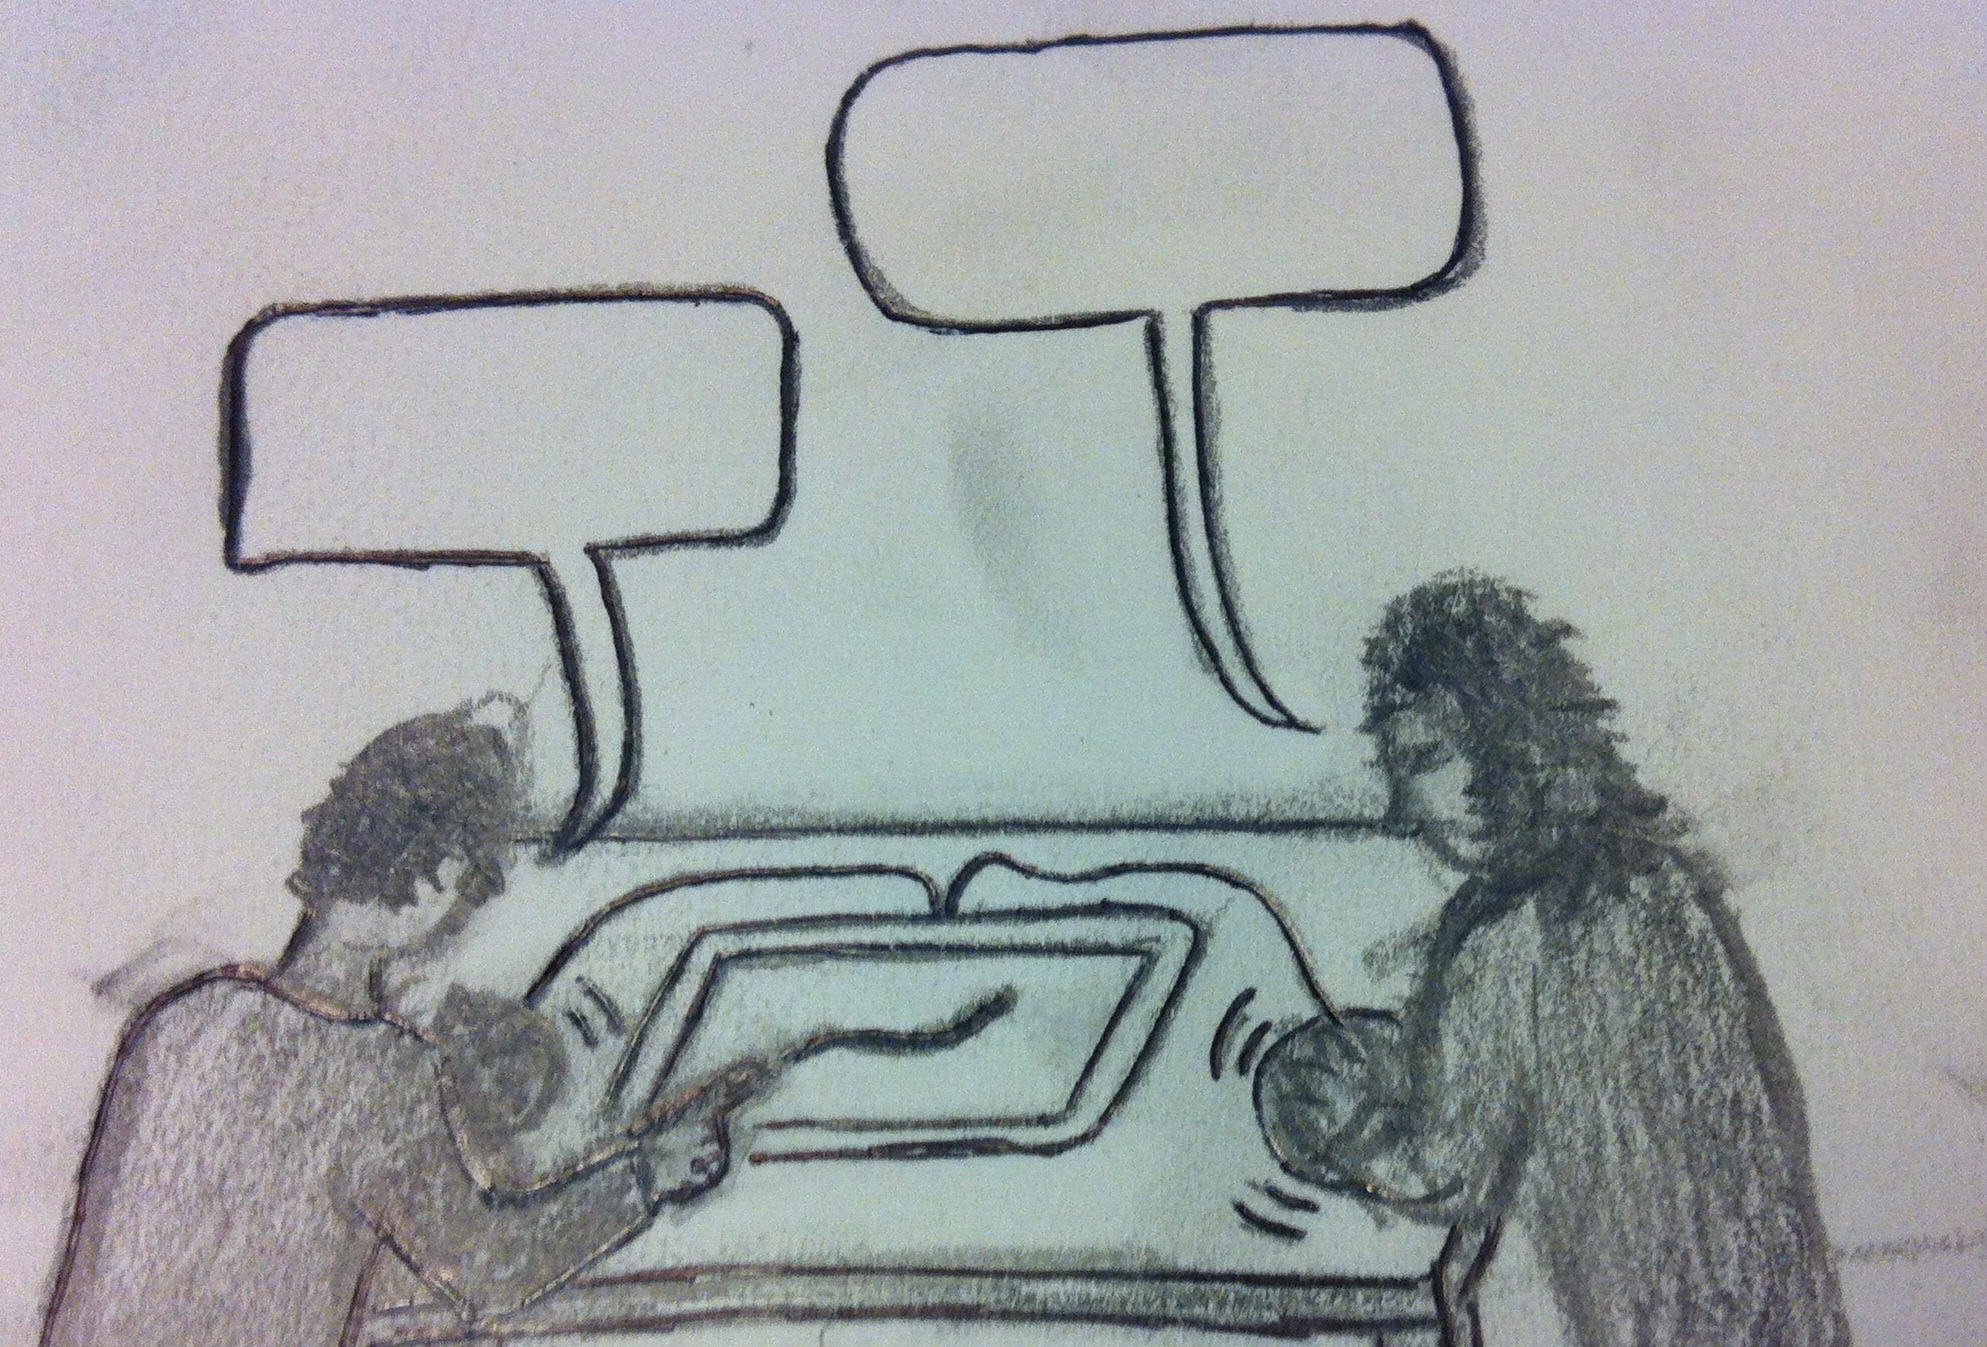
\includegraphics[width=0.4\textwidth]{HapticInstrumentConceptSketchRough} 
%   \caption{Concept Sketch of the Haptic Instrument}
%   \label{fig:HapticInstrumentConceptSketch}
%\end{figure}

\begin{figure}[h] %  figure placement: here, top, bottom, or page
   \centering
   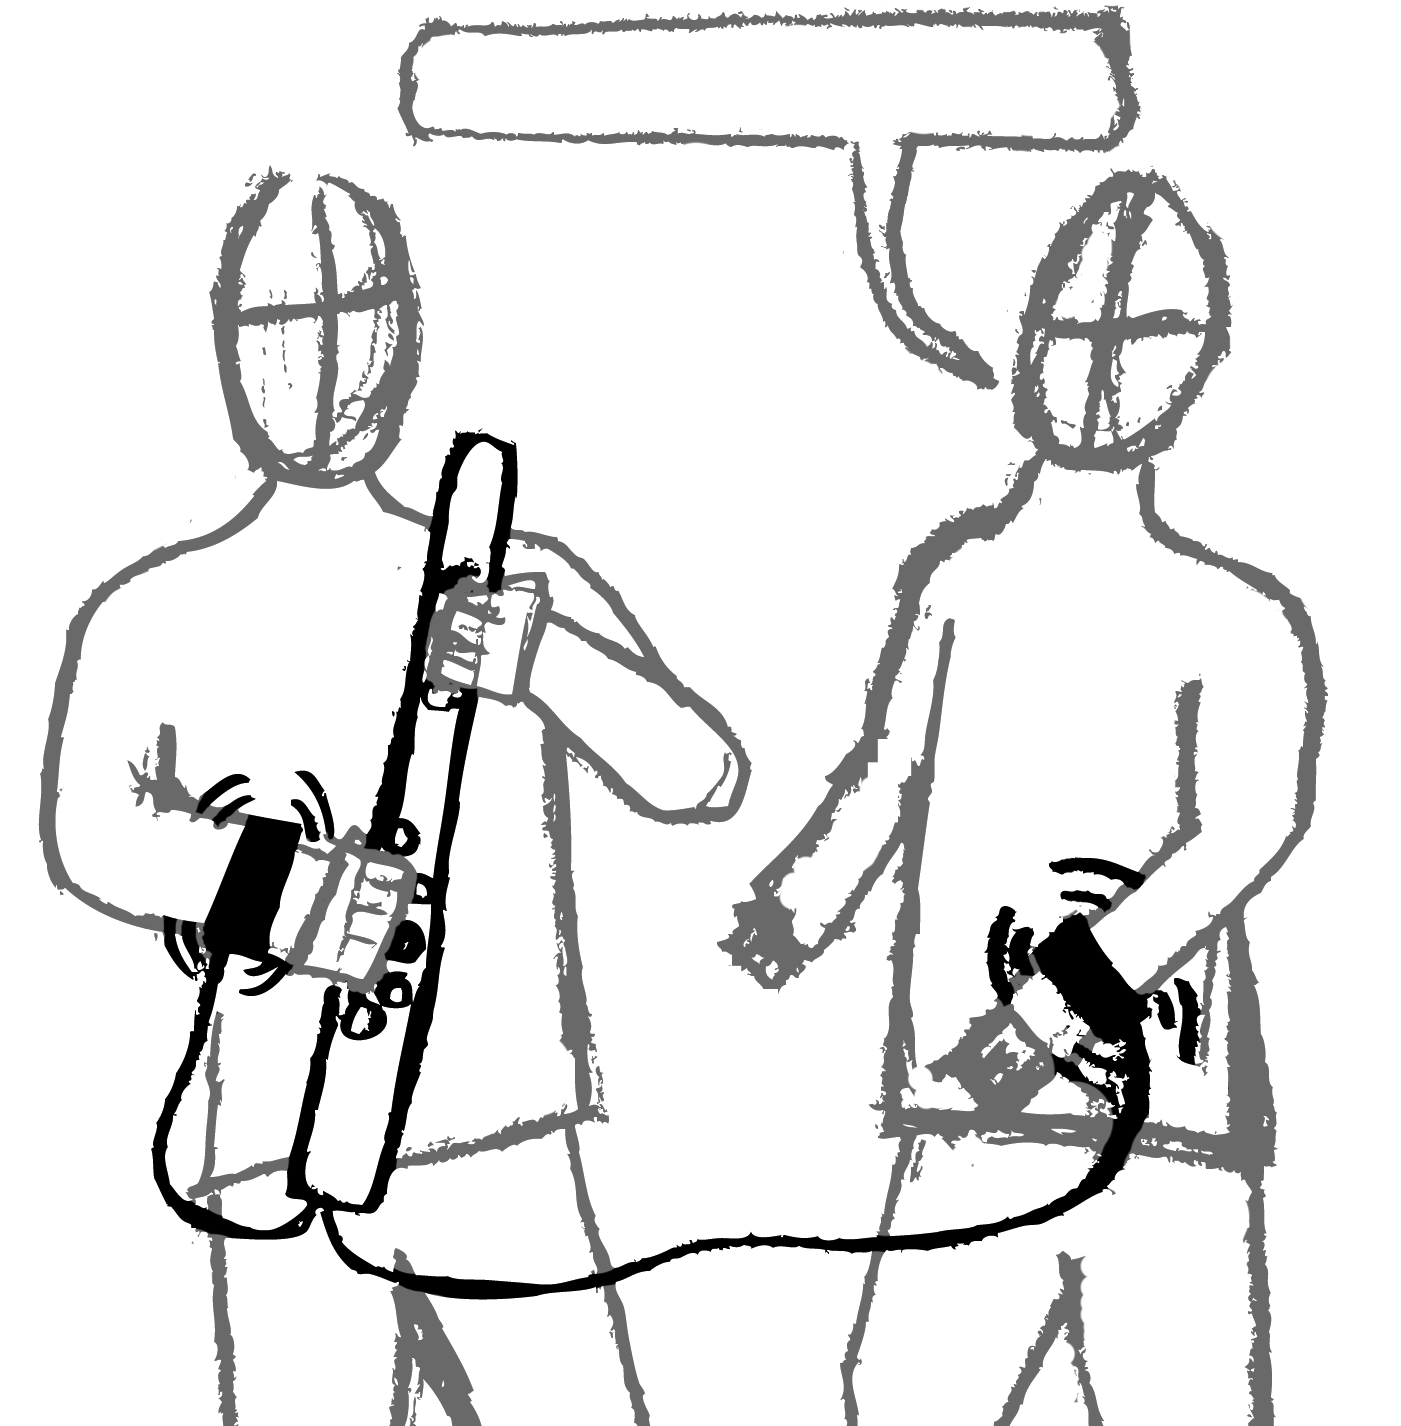
\includegraphics[width=0.5\textwidth, height=2.3in]{haptic-instrument-concept-sketch-sax-small-traced-squarer} 
   \caption{Concept sketch of a haptic instrument. Both users experience the same sensation, controlled in real-time.}
   \label{fig:HapticInstrumentConceptSketch}
\end{figure}

The Haptic Instrument case study\footnote{Published in Haptics Symposium 2014 \cite{Schneider2014} and at a CHI 2014 workshop \cite{Schneider2014b}.} is a first exploration into building a vibrotactile design tool, looking at design activities of exploration and informal sharing.
Through it, we investigate the role of real-time feedback and synchronous collaboration on haptic experience design, using participants with some haptics experience, serving as proxies for haptic experience designers.
Conventional haptic design tools contain a slow iteration, requiring programming or rendering before playback.
Using a music composition metaphor (as in~\cite{Lee2009}), we are writing music without ever playing a note: composing a work in its entirety, then listening to the result before making changes.
In contrast, musicians often use their instruments as a tool for serendipitous exploration when designing music.
%and can draw upon musical theory.
Furthermore, music is collaborative, with communication facilitated by a reference point of a sound.
%Touch, however, is a personal, local sense, making it difficult to discuss stimuli.


%Facilitated exploration and collaboration % in haptic design should 
%should streamline the haptic design process and inform a guiding 
%theory, analogous to those for musical composition. % theory. % vague?
%% With eased exploration, 
%Designers will attain fluency with new devices and control parameters,
%while collaborative elements % should help communication, but also 
%% could prove key to developing this theory.
%%Previous approaches have all been single-user design tools.
%%We suspect that adding a collaborative element is the key to developing these languages
%will get people designing in groups.  A usable haptic language may emerge from their dialogue.
%% they use to collaborate might emerge naturally from the collaborative interactions.


%Furthermore, recent work has identified major communication barriers in industry. Designers of haptic sensations are forced to carry examples of different textures or dynamical systems to make their point to stakeholders.



Our approach is to directly use a \emph{haptic instrument}, inspired by musical instruments but producing (for example) vibrotactile (VT) sensations rather than sound (\autoref{fig:HapticInstrumentConceptSketch}).
Haptic instruments are intended to have two main uses: they provide real-time feedback to the user to facilitate improvisation and exploration, and produce haptic output to multiple users as a \emph{what-you-feel-is-what-I-feel} (WYFIWIF) interface.
This allows for a dialogue that includes a haptic modality: haptic instruments create a shared experience of touch, allowing for a common reference point.


% when two or more people are talking.
%We hope that haptic instruments will not only prove to be useful tools in their own right, but also allow for a haptic language to emerge naturally from the dialogue surrounding this shared experience.
%We developed a vibrotactile instance, mHIVE (mobile Haptic Instrument for Vibrotactile Exploration), as a platform to investigate this concept.


%Our main contributions are:
%\begin {itemize}
%	\item A definition of the haptic instrument concept \& design space.
%	\item A fully-working haptic instrument (mHIVE).
%	\item The novel application of an established psychological methodology, phenomenology, to investigate mHIVE's interface and subjective tactile experiences.
%%	rather than psychophysical thresholds.
%	\item Preliminary results from a qualitative study that show mHIVE supports exploration and collaboration, and implications for the design of future haptic design tools.
%\end{itemize}

%%\noindent
%In this paper, we first cover the related work of haptic design tools and haptic language,
%%, identifying the progress so far in haptic design tools and conceptual models.
% then define the haptic instrument, its requirements, features, and design space.
%We report the design of mHIVE,
%% and the feedback we have encountered.
%our methodology, and preliminary results, and
%% investigating both the experience of using mHIVE and the language used to describe haptic phenomena.
% conclude with future directions for haptic tool design and research into a haptic language.
%%, and a vision for how haptic instruments can be used to develop a conceptual framework, the analogous musical theory for haptic sensations.
%%
%%\begin{itemize}
%%	\item Haptic jazz is a rich metaphor
%%	\item Haptic ``lead sheets" instead of scores
%%	\item improvisation
%%	\item social
%%\end{itemize}

\begin{figure*}[Htb]
   \centering
   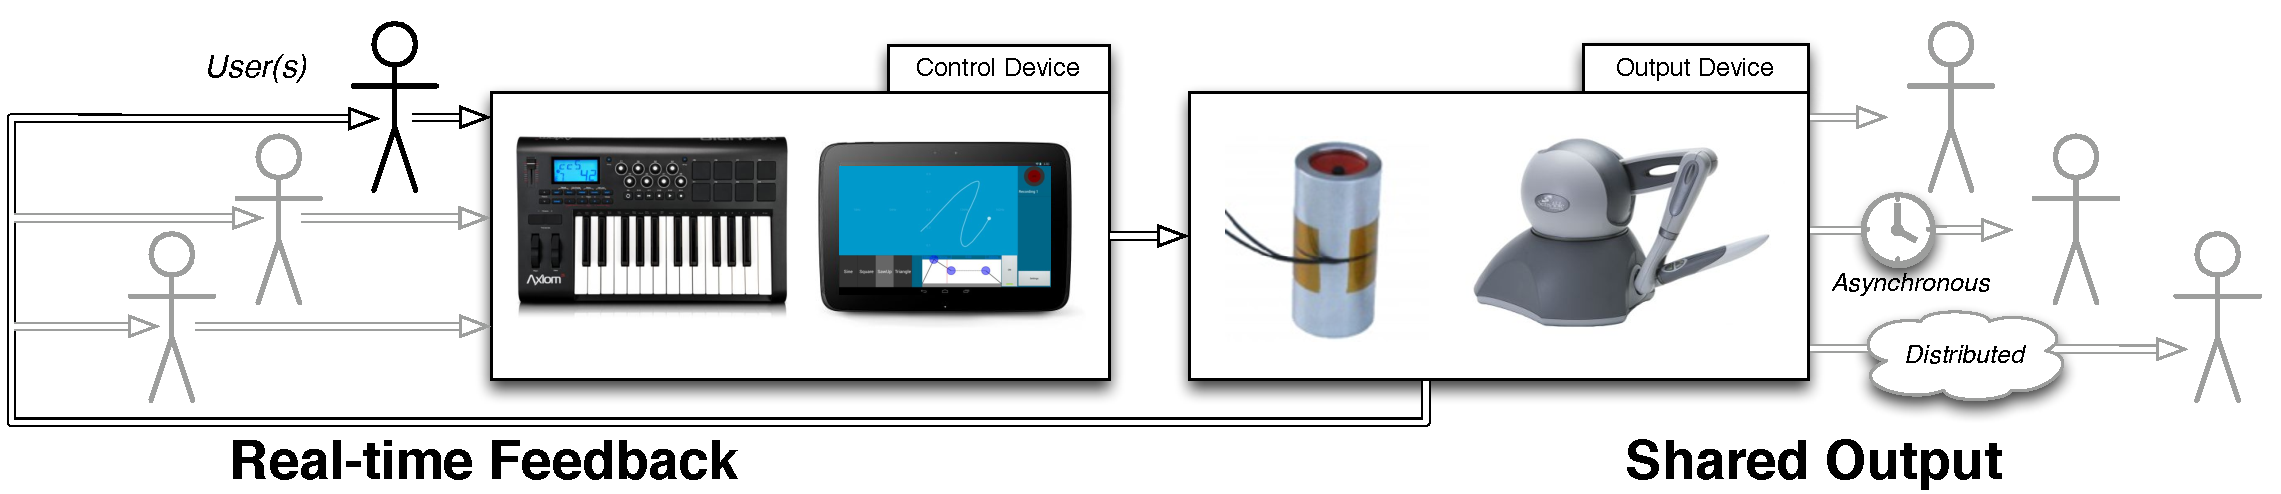
\includegraphics[width=\textwidth]{haptic-instrument-concept-horizontal4-small} 
   \caption{The haptic instrument concept. One or more people control the instrument, and receive real-time feedback from the device. Any number of audience members can feel the output in real time as well. Control methods can vary, from traditional musical control devices (such as the M-Audio Axiom 25, used in preliminary prototypes) to touchscreen tablets (used in mHIVE). Output devices vary as well.}
   \label{fig:HapticInstrumentConcept}
\end{figure*}




%Finally, we draw inspiration the Logo, which uses the ``transitionary object" of a turtle \cite{Papert1980}??? to aid users in making  to communicate experience, live coding ? Programming by example, haptic camera line of thought?


%%%%%%%%%%%%%%%%%%
%
% SECTION: Defining the Haptic Instrument
% 
%%%%%%%%%%%%%%%%%%
%\section{Defining the Haptic Instrument}
%We define a haptic instrument as a tool for general manipulation of one or more haptic (tactile, force-feedback, or both) devices that provides real-time feedback to anyone controlling the device, and can produce identical shared (WYFIWIF) output to all users to facilitate discussion and collaboration.
%Manipulation can include ideation, exploration, communication, recording, refinement, and articulation.
%Manipulation can be for utilitarian purposes (\emph{e.g.}, designing haptic notifications) or artistic expression (\emph{e.g.}, a haptic performance).
%Output devices can be purely output, or interactive.
%Furthermore, although haptic devices must be involved, multimodal experiences could easily be created by combining a haptic instrument with auditory or visual output.\footnote{One could even imagine a multimodal instrument such as Asimov's Visi-Sonor \cite{Asimov-Foundation-and-Empire} or its parody, Futurama's Holophonor \cite{Futurama-33-ParasitesLost}.}


%\begin{figure*}[htb]
%   \centering
%   \begin{minipage}{0.65\textwidth}
%	   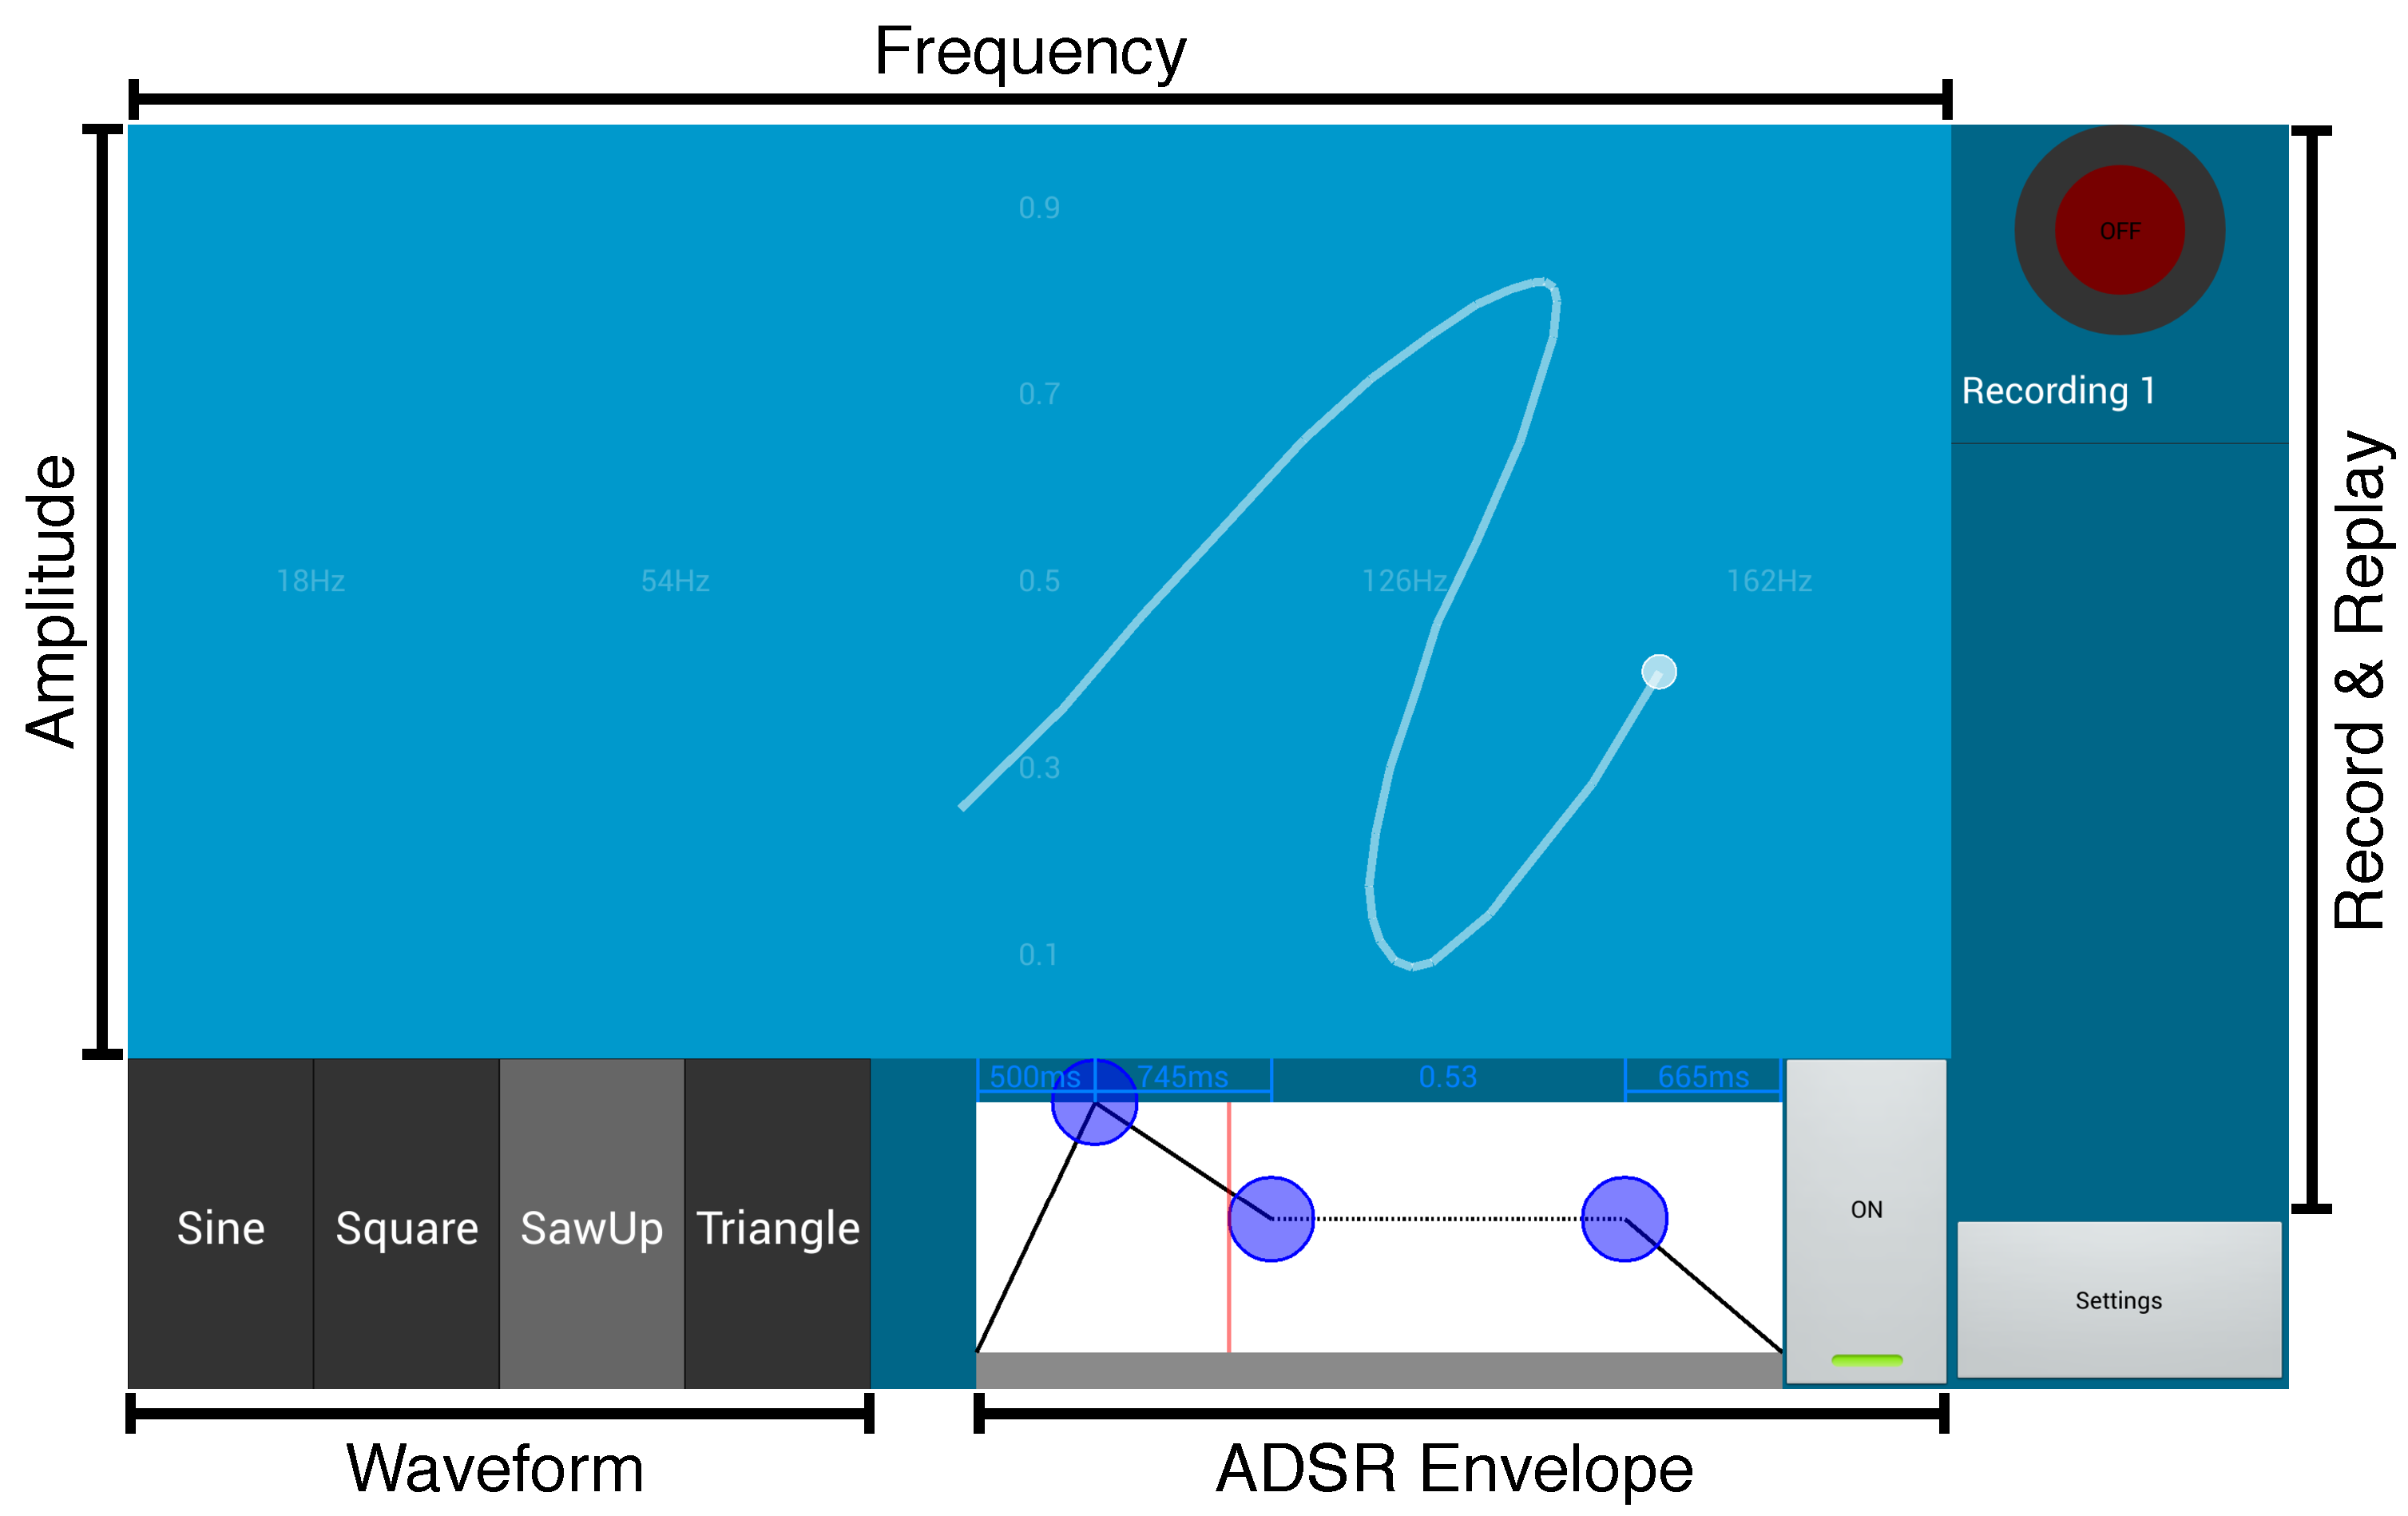
\includegraphics[width=\textwidth]{mHIVE-screenshot-labeled-2013-08-13} 
%	   \caption{mHIVE interface. Primary interaction is through the amplitude-frequency view, where visual feedback is provided through a circle (current finger position) and a trail (two seconds of previous interaction history).}
%	   \label{fig:mHIVE}
%    \end{minipage}
%    \hspace{1cm}
%   \begin{minipage}{0.25\textwidth}
%	   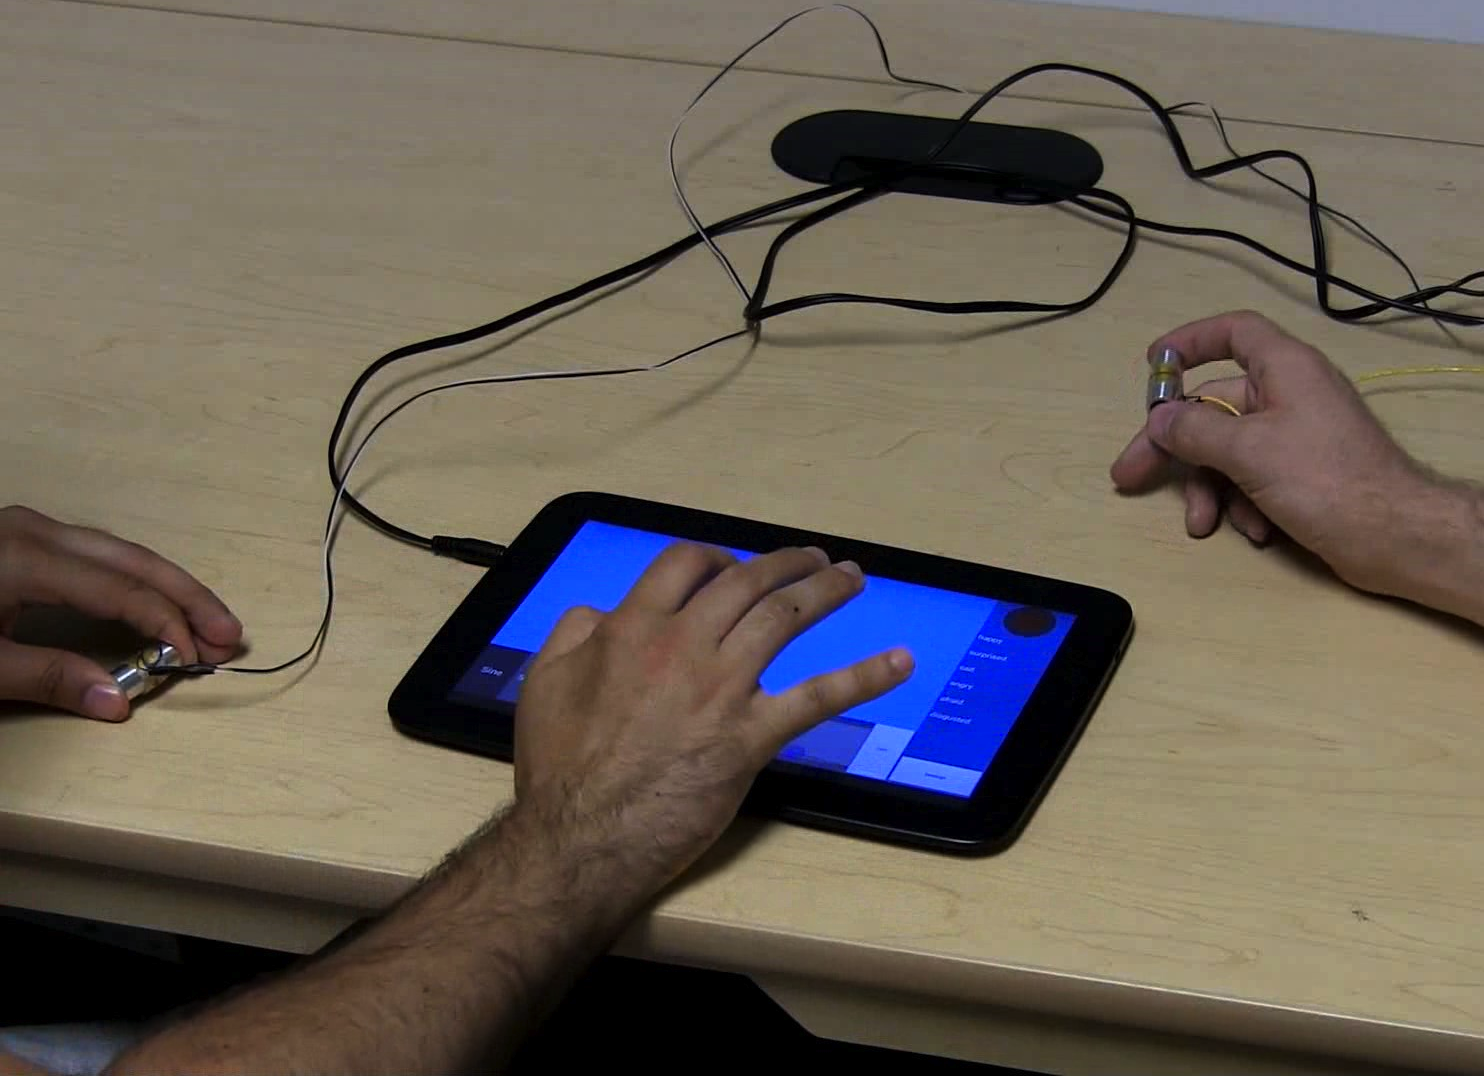
\includegraphics[width=\textwidth]{mHIVE-study-setup-cropped} 
%	   \caption{Study setup. The participant (left) controls the device while feeling the sensation; the interviewer (right) feels the same sensation on an identical output device.}
%	   \label{fig:StudySetup}
%    \end{minipage}   
%\end{figure*}





%%%%%%%%%%%%%%%%%%
%
% SECTION: mHIVE
% 
%%%%%%%%%%%%%%%%%%
\section{Design}

%%%%%
%SubSection: Design Dimensions
%%%%
%\subsection{Design Dimensions}
%Though haptic instruments by definition provide real-time feedback have shared-output, there are several main design dimensions that can be considered in a haptic instrument (outlined in \autoref{fig:HapticInstrumentConcept}).
%Note that haptic instruments can occupy multiple positions on these dimensions.
% Though haptic instruments by definition provide real-time feedback \kmEdit{??} have shared-output, 
There are several main design dimensions that can be considered in a haptic instrument (outlined in \autoref{fig:HapticInstrumentConcept}).
A haptic instrument can occupy multiple positions on these dimensions.
%; a haptic instrument could allow for both synchronous and asynchronous collaboration.

%\begin{description}

	\strongitem{Asychronous/synchronous}
%	Because of the shared-output,
%A haptic instrument collaborative.
Though a haptic instrument must provide real-time feedback, its collaborative (shared-output) aspect could be either synchronous (by having multiple people experience the real-time output) or asynchronous (by allowing for recording and playback, important for design).
%Indeed, recording is critical when creating musical pieces.

	\strongitem{Collocated/distributed} A haptic instrument's output could be present only for users in the same room, or be broadcast over a network to people around the world. For example, multiple mobile devices could all display identical output in a distributed manner.

	\strongitem{Private/shared %KM suggested collaborative, not going with it because of our use of "collaborative" elsewhere
control} A haptic instrument's control % interface 
 could be private (operated by a one person at a time) or shared (multiple users control the display). 
Shared control could be collocated or distributed (\emph{e.g.}, a web interface and shared object model).
	
	\strongitem{Output mechanism} Each haptic instrument will control a haptic device, which has its own mechanism for providing a haptic sensation (\emph{e.g.}, vibrotactile sensations). Because haptic devices can be complex and combine multiple mechanisms, this is a large space in its own right. Characterizing the different display mechanisms is something that we must leave to future work. Suffice it to say, a haptic instrument will be different depending on its output device.

	\strongitem{Number of haptic instruments or output devices}
	One consideration is whether a haptic instrument is intended to operate alone, or with other haptic or multimodal instruments.
%	\kmEdit{slc} % Don't you need to mention also, multimodal design? jam the haptic channel along with the auditory?
	One can imagine haptic jam sessions for inspiration and ideation, or even form haptic bands for artistic expression.
	This is highly related to private/shared control -- there is a fine line between several identical haptic instruments with private control, and a single haptic instrument with shared control and several output devices. Note that a haptic instrument may involve several devices to produce shared-output.

	\strongitem{Control mechanism} Similarly, a haptic instrument could be controlled in a variety of ways.
	From musically-inspired MIDI controllers to smartphone applications, we envision a wide variety of control methods.
%	Even a real-time programming environment might be appropriate for complex interactive sensations.
%	One should note that the control mechanism must work with the output device's paradigm.
	Even a real-time programming environment might be appropriate for complex interactive sensations,
	so long as the control mechanism works with the output device's paradigm.
%	 likely depend on the display mechanism, as many display mechanisms required their own paradigm for control.

%\end{description}
%
%We expect that haptic instruments could provide both immediate and long-term value.
%% In the short term, 
%We hope haptic instruments will improve the design process immediately, by supporting exploration and collaboration.
%% won't just be valuable on their own, but might produce emergent value.
%%We also expect that there will be other valuable results that are emergent from.
%%We expect that exploration will help designers quickly internalize the meaning of different control parameters for a given device.
%%of different display mechanisms and the parallel differences in control paradigms.
%%Collaboration, on the other hand, could develop an explicit conceptual model or language analogous to musical theory that could aid haptic designers.
%Over time, their use could lead to a natural, emergent design language valuable in its own right.
%One can also imagine a general tool composed of several virtual haptic instruments, much like digital musical synthesizers.
%
%%User stories, requirements?

\begin{figure}[Htb]
   \centering
%	   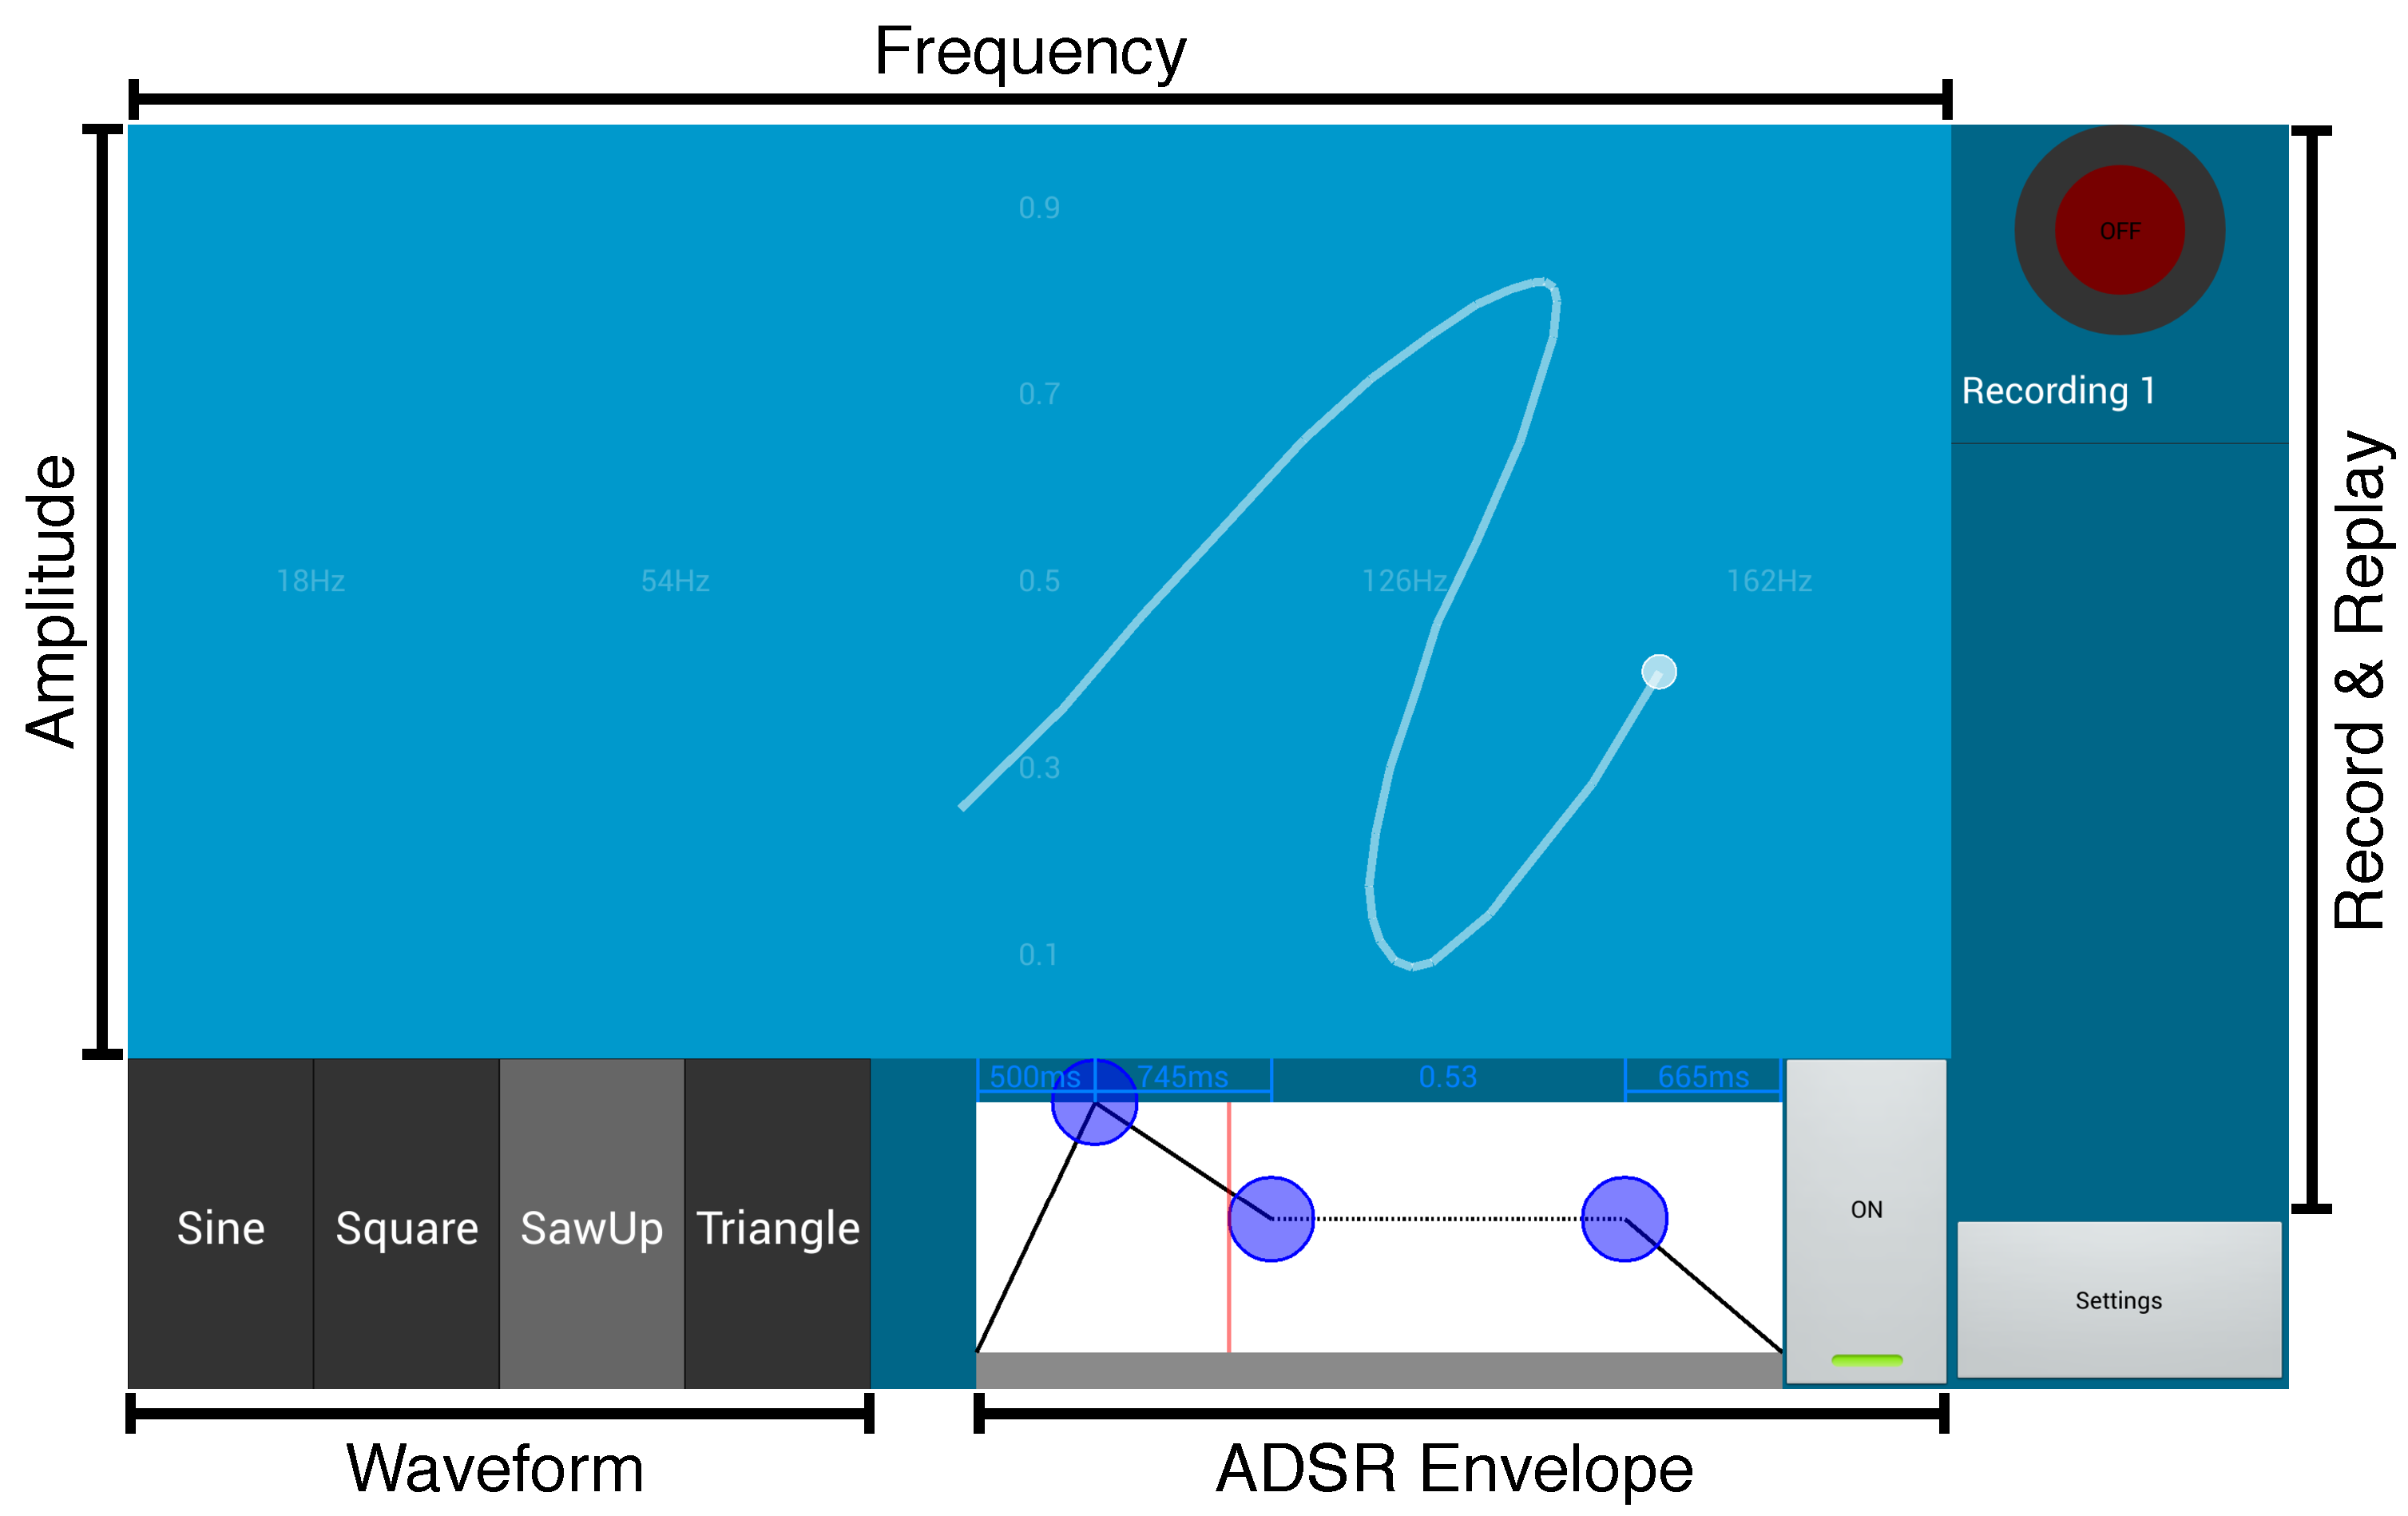
\includegraphics[width=0.43\textwidth]{mHIVE-screenshot-labeled-2013-08-13} 
	   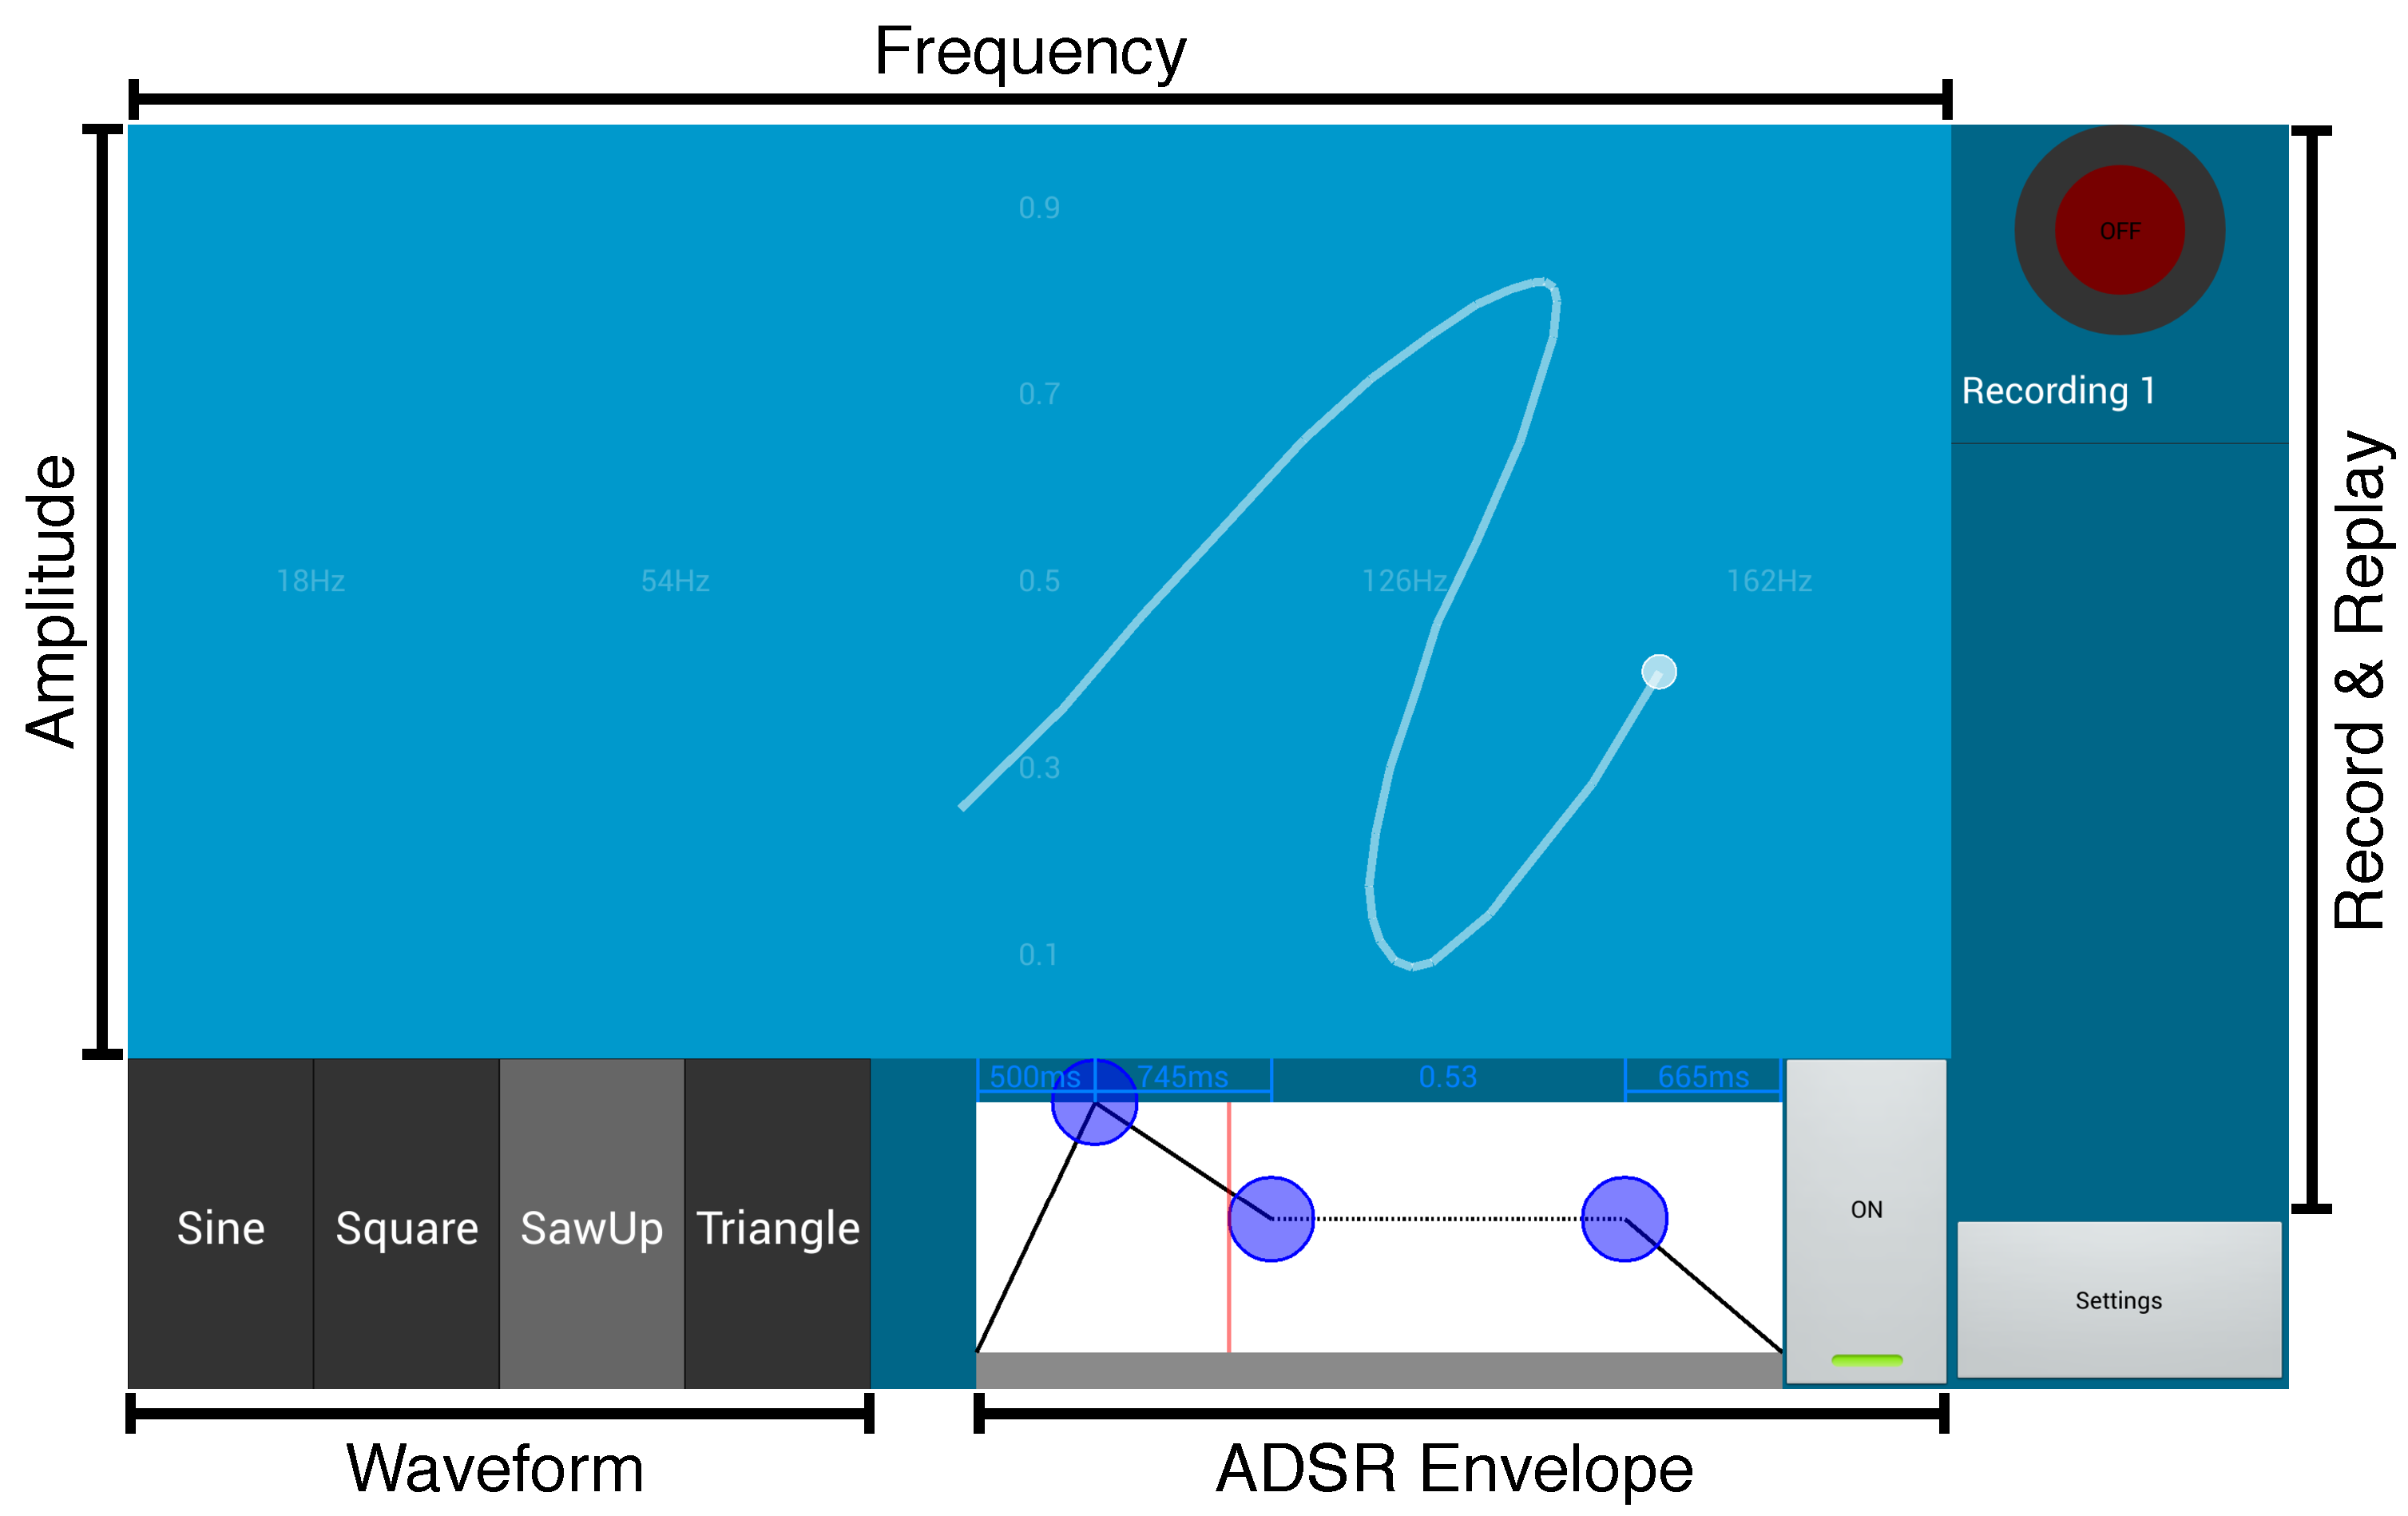
\includegraphics[width=0.7\textwidth]{mHIVE-screenshot-labeled-2013-08-13} 
	   \caption{mHIVE interface. Primary interaction is through the amplitude-frequency view, where visual feedback is provided through a circle (current finger position) and a trail (interaction history).}
	   \label{fig:mHIVE}
    \end{figure}



\subsection{mHIVE}%, a mobile Haptic Instrument for Vibrotactile Exploration}
We developed mHIVE, a mobile Haptic Instrument for Vibrotactile Exploration, to begin to explore how a haptic instrument should work and what it should do (\autoref{fig:mHIVE}).
% , we  developed a prototype, mHIVE (mobile Haptic Instrument for Vibrotactile Exploration,
%
%\footnote{Our first, low-fidelity prototype was named HIVE, before we switched to developing on a mobile platform. }
%
% mHIVE is a collocated, synchronous, mostly private control haptic instrument that controls 2 vibrotactile actuators
mHIVE is a collocated, synchronous haptic instrument for a single user. It accommodates shared display via dual
Haptuators~\cite{Yao2010}
and is operated with a single-touch tablet-based interface for direct manual control (\autoref{fig:hapticinstrument:StudySetup}). 
mHIVE is designed for for VT
% We chose this as a simple first attempt at a haptic instrument: vibrotactile 
sensations, which are common, do not require interactive programming, are controlled through waveforms (analogous to music), and their low-level control parameters are well understood.
%As well, they are commonly used in commercial devices, such as smartphones.
%Using a touchscreen % interface 
%allowed %was chosen for 
%direct manual control, similar to most musical instruments. % of the control parameters.
%: early desktop prototypes were awkward.



mHIVE offers real-time control of frequency, amplitude, waveform, envelope, duration, and rhythm, identified as the most important parameters for VT sensations \cite{Gunther2002,Brown2006a,Brown2006,Brewster2004, Rovan2000}.
mHIVE is implemented in Java using the Android SDK \cite{AndroidOpenSourceProject2012}, and the FMOD sound synthesis library \cite{fmod2013} to produce sounds, sent to two or more Haptuators through an audio jack.
%Thus, mHIVE is effectively a sound synthesizer designed for tactile sensations.
We deployed mHIVE on an Android Nexus 10 tablet running Android 4.2.1.



%mHIVE allows for control of frequency (5-180Hz, determined through piloting) and amplitude (0 (min) to 1 (full)) by drawing on a main input canvas.
%The ADSR filter can be toggled on or off by an adjacent button.
%As well, mHIVE allows for the user to record their input for later play back.
%Recording captures all input events, including waveform selection, ADSR manipulation, frequency/amplitude input, and even recording playback.

%%%%%%%%%%%%%%%%%%
%
% SECTION: Study Methodology
% 
%%%%%%%%%%%%%%%%%%
%\clearpage
\section{Study}

%%%%%%%%%%%%%%%%%%
%
% SECTION: Study Methodology
% 
%%%%%%%%%%%%%%%%%%
%\clearpage
% With mHIVE built, 
We conducted a qualitative study to investigate two questions.
%\km{Q1/Q2?slc} % consider numbering them for more structered reference later. gives a bit of formalism.
First, is mHIVE an effective tool for the expression, exploration, and communication of affective phenomena?
Second, what language, mental models, and metaphors do people use to describe vibrotactile sensations, and how do they relate to mHIVE's low-level control parameters?

\begin{figure}[Htb]
	\centering
%	   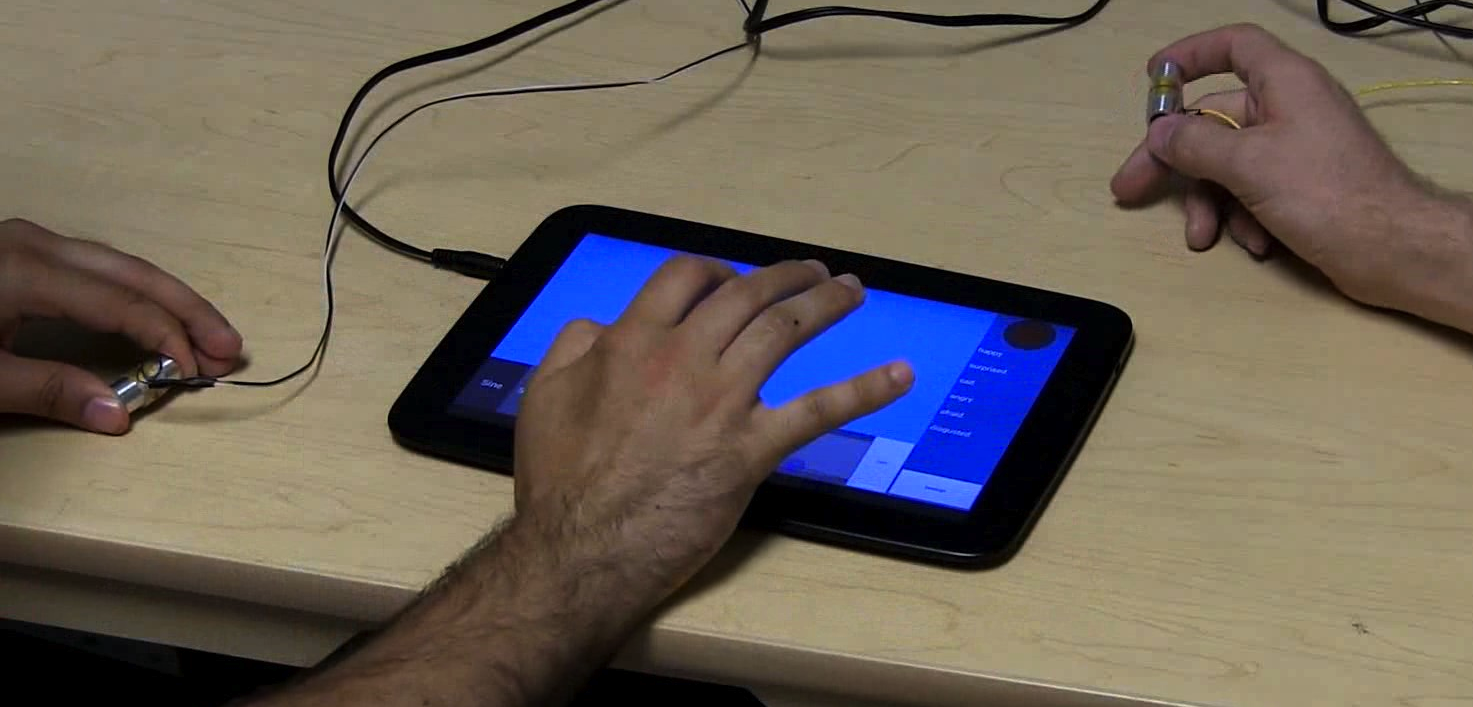
\includegraphics[width=0.32\textwidth]{mHIVE-study-setup-cropped2} 
	   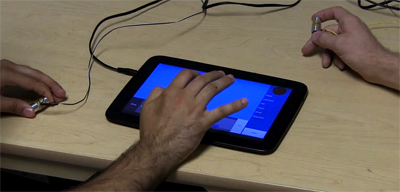
\includegraphics[width= 0.65\textwidth]{mHIVE-study-setup-cropped2small} 
	   \caption{
	   Study setup. Both the participant (left) and the interviewer (right) feel the same sensation as the participant controls mHIVE.
%	   The participant (left) controls mHIVE while feeling the sensation; the interviewer (right) feels the same sensation.
}
	   \label{fig:hapticinstrument:StudySetup}
\end{figure}

%\subsection{Procedure}
One researcher collected and analyzed data using the Stevick-Colaizzi-Keen method as described by Moustakas \cite{Moustakas1994}.
Our 1-hour open-ended interviews
%with four participants, all with haptic experience.
used the following protocol:
\begin{enumerate}
	\item Ask the participant for their background: occupation, experience with touchscreens, haptics, music, and video games.
	\item Demonstrate mHIVE to the user, and invite them to explore while thinking aloud to describe the sensations they feel.
	\item Probe the design space by asking participants to explore different control parameters, and to explore their metaphors (\emph{e.g.}, if the participant describes a sensation as ``smooth", R1 would ask them to try to produce a ``rough" sensation).
	\item Ask the participants to produce sensations for the six basic cross-cultural emotions documented by Ekman \cite{Ekman1992}, and rank how well they think their sensation represents the emotion on a 4-point semantic differential scale (Very Poorly, Somewhat Poorly, Somewhat Well, Well). This was done both as an elicitation device to gather a wider range of interactions with mHIVE, and to directly investigate a design task.
	\item Set the Haptuators down, and ask the participants to describe their experience of working with mHIVE in as complete detail as possible to evaluate the device itself.
\end{enumerate}

\noindent
R1 conducted the interviews and analysis, which required specialized knowledge of mHIVE.
%, and inductive nature of analysis did not allow for other researchers to cluster separately.
% Because clustering was conducted and not coding, 
%\kmEdit{Because we conducted clustering rather than coding,??}
Scores of inter-rater reliability common with other qualitative analyses (\emph{e.g.}, grounded theory \cite{Corbin2008}) are inappropriate and unavailable, as we did not conduct deductive, low-level coding.
To improve reliability,  R1's documented experience was analyzed first, and then consulted during analysis to remove bias (\emph{e.g.}, to not use terms only used by the experimenter).
%documented and analyzed his own experience with the device, which was considered when conducting analysis.
%we present here separately from other results to clearly demarcate the researcher's biases and preconceptions.
%Even so, results are grounded in empirical data, shown by quotations representing the clusters.
%Participants will also be contacted after analysis to provide feedback on our initial conclusions \textbf{TODO}.

%%%%%%%%%%%%%%%%%%
%
% SECTION: Results
% 
%%%%%%%%%%%%%%%%%%
\section{Results}

We sought participants with experience designing haptics as a proxy for expert designers for our initial study.
Four participants were recruited through email lists and word-of-mouth (P1-4, three male), and were all in the age range of 26-35 with self-reported occupations including graduate students or post-docs in information visualization, HCI, and human-robot interaction.
All had experience working with haptic technology, and (because of this requirement) all knew the main researcher in a professional capacity, although only P2 had seen earlier prototypes of the haptic instrument.
The small sample size, typical for phenomenological studies \cite{Creswell2013}, was appropriate for the rich data we wanted.
Data collection ended when we achieved saturation of new results, and had a clear direction for our next iteration.

%determined by saturation of new data: when we stopped encountering new data, we stopped recruiting participants.

%Analysis revealed several themes among the participants, particularly about the device's role in the design process, a tendency towards audio metaphors or concrete example-based metaphors, and a notion of enjoyable sensations vs. non-enjoyable sensations.
%As well, usability concerns are reported, suggesting implications for the design of future haptic instruments.

%
% Subsection: Reflections
%
%\subsection{Researcher Reflections and Experience}

%\emph{Note: This section is written by the researcher who led development of mHIVE and conducted the interviews and analysis.}

%%Researcher eval v1
%%As the principle developer of mHIVE, I have a unique outlook on the device.
%%I entered the study with planned improvements derived from piloting.
%%Deliberate exploration of the device revealed a number of takeaways which I will report here.
%%Some are may be similar to the experience reported by study participants, and some are specific to me.

%%Because I built the device, I understood the underlying mental model, and thus found mHIVE to be \q{very intuitive,} and \q{very helpful.}
%%I \q{enjoyed using it.}
%%I found visual trace and ADSR envelope to be \q{helpful.}
%%In particular, ADSR was very \q{important} to me, and was useful to \q{soften the edges} of the sensations.

%%However, I do not believe that mHIVE is perfect.
%%First, the addition of multitouch is \q{important.}
%%I found it was tricky to \q{juggle both hands}, feeling the output while simultaneously controlling the interface.
%%I have mixed feelings about the recording feature. Though I found it \q{helpful the one time} when developing the surprise sensation, I only used it once and feel that it \q{needs work.}
%%I had originally though that the recording feature needed a stop button, but \q{I didn't used it enough to notice} any lack of such a feature.

%%Finally, I found myself changing waveform and ADSR infrequently; it was \q{easy to leave something in place.}
%%Overall, I felt that mHIVE was \q{an exploratory tool} rather than a tool for \q{refinement.}
%%It would be best suited to exporting icons to \q{another application or another task.}

%%researcher eval v2
%Because I built the app, I understood the underlying system model. Because of this, I enjoyed using it, thought it was helpful, and found it intuitive and easy-to-use. I thought visual trail was very nice and helpful, because I could see where it was, and that ADSR was important, especially for a ringing sensation. I experienced unexpected sensations, calling them weird.

%Of course, because I was using an early prototype, there were still some interface-level refinements I thought were important to make. Some of these became less important as I interacted with the device. I thought that it needed a button to stop replay, but because I only used the record/replay feature once when exploring the device and didn't notice the lack of a stop button, I thought it was fine. Interacting with the device, multitouch emerged as an important feature to try. Overall, I though mHIVE was suited for exploration but not refinement, and thought it might be a good idea to record haptic icons and export them to another application.

%Low frequency sensations stood out to me as oscillating, pushes, thumps or hits (with the square wave), and felt like a watch or subwoofer. I described some low-level sensations with onomatopoeias, including djoo djoo djoo, wub wub wub, tick tick tick tick. ADSR allowed sensations that felt like soft bells, and that made me picture the sound of an ocean swelling. I made frequent analogies to technology: lasers, boat motors revving, and zippers, and could hear higher frequencies, comparing them to mosquitos buzzing or high pitched whines like an plane engine.

%I also used tactile metaphors, tingly, strained, taut, grainy, gritty, and rumbly. Triangle and sine waves became more forceful while square and sawtooth waves became stronger. Higher frequencies were smooth, like a constant ringing, and sometimes aggressive, viscious, on edge, or even painful (on one occasion).

%
% Subsection: Themes
%
%\subsection{Themes}
Here we report the three major themes that emerged during analysis: % possibly: use this spot to help with the expansion on methodology, reinforcing that it was systematic not biased, clearly a concern of the reviewers.}
%
 mHIVE's success as a haptic instrument, mHIVE's limitations that reveal more detail about the haptic design process, and the use of language in the study.

\theme{mHIVE Succeeds as a Haptic Instrument}

%mHIVE achieved its goals of exploration and communication. 
Our results suggest that mHIVE can be effective for exploration of a design space, and communication in the haptic domain. % This section does come across as one-sided. Being critical: the goal of exploration/communication is broad and loose (a low bar?) and many statements could be used in support of it. Can you balance with statements that either countered it (showed where improvement was needed) or establish limits? Most helpful now is that you break it down into sub-themes.
Overall, mHIVE was well received, seen as a novel and promising tool.
\nq{1}{I definitely liked it},
\nq{2}{I think there should be more devices like this for designing haptic icons}.
%\nq{3}{It was fine. I mean I guess at the high level, it's relatively easy -to-use}
%\nq{4}{it's a nice, uh, nice sandbox to play in}


\strongitem{Serendipitous exploration}
Participants reported that mHIVE was best served to explore the design space, generate a number of ideas, and try things out.
Serendipitous discoveries and exclamations of surprise were common.
Participants were able to \nq{2}{accidentally stumble upon something} as they explored the device.
%	\nq{1}{what's that going to be like},
%	\sq{maybe something like this�}
%	\nq{2}{it's not like you know, uh, everything in advance, it's not like you're trying to mimic something, you're trying to put random things together and see what meanings you can extract out of it}
	\sq{I felt I could get a large variety},
	\nq{3}{I could easily play around with the high-level to find out what was neat}.
%	\nq{1}{Ooo, that's kinda cool}.

%In addition, mHIVE let the participants "accidentally stumble upon something" (P2), revealed through expressions of surprise when feeling interesting sensations:


%	\nq{2}{Yeah, you feel like, oh this is interesting}

%	\nq{3}{That's an interesting kind of effect there}

\strongitem{Communication}
mHIVE %was not just a tool for exploration, but also communication as it 
established an additional modality for dialogue.
%Participants referred to sensations as a deictic channel, essentially using the device in a manner analogous to gestures.
The dual outputs created a shared context, demonstrated by deictic phrases: the additional context of the vibrotactile sensation was required to make sense of the statement.
The use of ``that" and ``there", reminiscent of the classic ``Put That There" multimodal interaction demo \cite{Bolt1980} indicate a shared reference point was established from the haptic instrument.
\nq{3}{So there'd be like, (creates a sensation on the device), which is pretty mellow}.

In particular, P4 successfully communicated the sensation of sleepiness to the R1, by asking whether R1 could guess the sensation.
\nq{4}{Can you guess it?} \namedquote{R1}{Sleepy?} \nq{4}{Yeah. Pretty good}.
The dialogue worked as a two way channel, as R1 was able to phrase questions using the device.
%, and communicate the sensation of surprise to P4, or pose a question to P2.
	\nq{2}{It was different} \namedquote{R1}{How was it different?} \nq{2}{You delayed the first part, it felt new}.%, but when you make random moves}

Certain sensations, like a feeling of randomness, could only be felt when another person controlled mHIVE.
	\nq{2}{When someone else does it, I feel better, it's like, you cannot tickle yourself}.


%This was revealed especially when discussing a usability flaw in the device, a lag between touching the device and the output of the sensation:
%	\nq{2}{(taps on the device, demonstrating delay) you feel the delay?}
%In addition, the interviewer was able to phrase questions by using the device:
	
	
%	\theme{ADSR envelope has a learning curve}

%\strongitem{Learning curve}
%Like a musical instrument, mHIVE also has a learning curve.
%This is especially true with the ADSR envelope, which was unfamiliar to most participants.
%P4, a musician who had encountered ADSR envelopes before, was more familiar with the concept, but still felt that he could become more expert with mHIVE.
%Though a learning curve limits who can use the device, it might just mean a different target audience, such as experts rather than novices, or designers rather than end-users.
%%ADSR especially required more expertise than the other features:
%	\nq{1}{This little plot dude down here didn't make sense to me at all at first, once you explained it, it totally it did; I'm still not very confident in my ability to map between this plot and sensations, but I kinda get how it would work},
%	\nq{4}{I think it does require a bit of a learning curve}.
%%\nq{3}{I find this a bit harder just to perceptualize, but by the end I think I was starting to get a sense of how it worked, it took me longer than the other aspects to, clue into.}
%%\nq{4}{So I don't know if most people would take the time to use a tool like this to develop a range of different haptic signals for their phone, but this would be a great tool for a designer to use}
%%We suspect that ADSR would be used more heavily by expert users.
%However, some designers might still not want to use ADSR at all.
%\nq{3}{This attack and release, I find it the third most valuable thing [of four].}

%% P2 and found the control confusing when the sustain was 0 (\q{(sustain $<0$), I can control how long it vibrates}, \q{(sustain 0), it's like it dies, and, seems like, um, I dunno I'm less in control of this one}).

%%P4, with experience in digital music, immediately recognized the ADSR. TODO

\theme{Tweaking through Visualization and Modification}

During analysis, some key directions for future design emerged around visualization and control capabilities.

\strongitem{Inability to tweak}
Though mHIVE supported exploration and collaboration, we found % that mHIVE was not a general design tool on its own.
it was inadequate as a standalone design tool.
Few created sensations were considered to be final.
Many descriptions were hedged % with an ``I dunno," 
and in the design task, few sensations captured the emotional content well.%(\autoref{fig:design:bar:plot})
	\nq{1}{I dunno, maybe that's afraid?},
%	\nq{1}{Not bad\ldots I feel that one could do better}, \sq{My angry is somewhat disgusted}
	\nq{2}{Still felt that you can make them better},
	\nq{3}{To me that's more fuming (laughing) than it is angry}.
%	\nq{4}{I'm sure if I spent more time on this, I think we could play around a bit more with the design space.}
On some occasions, participants were certain about their descriptions.
\nq{1}{Sad, definitely down on the amplitude with sad\ldots oh that's totally sad. Yeah.}.
%, \nq{2}{Yeah. This is afraid.}
This was uncommon, and usually tied to discovering an ideal sensation during the design task.

%\begin{figure}[htbp] %  figure placement: here, top, bottom, or page
%   \centering
%   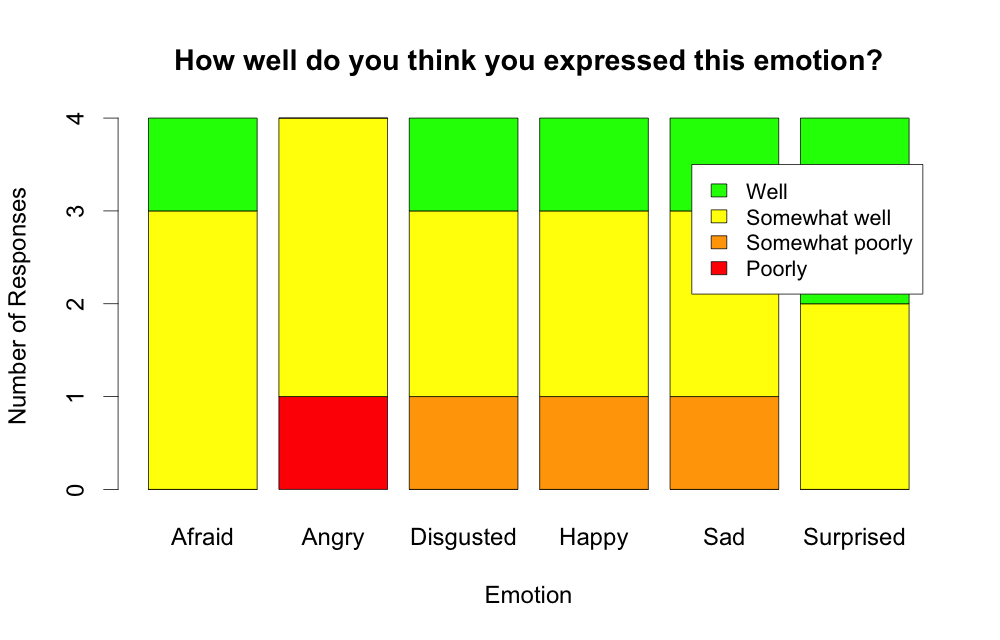
\includegraphics[width=0.47\textwidth]{mHIVE-BarPlot} 
%   \caption{Participant ratings of the confidence in their designs}
%   \label{fig:design:bar:plot}
%\end{figure}


%\strongitem{Memory and attention barriers}
\strongitem{More visualization and recording}
%Though the participants were able to create initial designs for sensations, they were unable to develop them.
Part of mHIVE's inability to support tweaking was due to cognitive limitations for both memory and attention.
Participants found it difficult to remember what they had tried before, % and found it difficult 
and to pay attention to the output % sensation 
while simultaneously controlling it. %the device.
%Participants found significant cognitive challenge in remembering what they had tried before
%	\nq{2}{I tried to recreate that but I couldn't create it exactly as it felt the first time}
\nq{3}{There's a lot of variables which, when I'm trying to compare between two configurations\ldots it was hard sometimes to remember what I had tried},
%if I've done something,
%\theme{Tactile Overshadowing, Looping is required}
%Participants unanimously expressed a desire to feel sensations without having to simultaneously control the device, allowing participants to focus on the sensations they were feeling. This was achieved either by using the recording functionality or the interviewer control mHIVE:
	\nq{1}{I definitely liked being able to feel a stimulus without having to implement it, you know, it allows me to focus more on what it feels like}.
%%	\nq{3}{it's bit hard to do, like I'm trying to go for what I'm imagining, it's hard to do it and feel it at the same time I guess?}
%%	\nq{2}{I tried to recreate that but I couldn't create it exactly as it felt the first time}
%%One thing all participants mentioned was a difficulty remembering what they had previously created or developed. This was partially alleviated by recording, but a desire for more history was deemed important:
%	\nq{3}{It was neat when I could play it back and be like, what did I do and I could see, oh I did that\ldots
%	%and then being able to see where it was was very useful, cuz that helped me in, in what I wanted to be able to kind of replay, like 
%	oh I remember doing something that might work in this situation}.

%This was especially true when the participants noticed a delay between touching the tablet screen and the haptuators activating.  \sq{Feels like there's a delay}, \nq{2}{If I don't look at your finger, I don't see the asynchrony}.

%\strongitem{More visualization and recording}
Participants suggested that although % though 
visualization and recording features helped somewhat %a little 
to overcome these limitations, more was needed. % they needed to be improved.
%All participants requested a further emphasis on recording through repetition or looping.
%This was intended to both aid memory and allow participants to focus on the sensation without worrying about controlling the device.
All  requested greater emphasis on recording through repetition or looping, both to aid memory and allow for focus on the sensation independent of device control. 

%
%\km{SLC***: simultaneous compose/review bad; fluid mode shifting good?} % KM: just struck me: does this undermine the key starting premise that we should be able to perceive the design output AS we create it? In fact, we're finding that this is cognitively too hard. Is it the same for music? Maybe what we have learned is that you need a little space, but not much; and perhaps it is more important that the cognitive effort and time elapsed in moving between composition and review is very streamlined - i.e. you do them separately, but the movement between modes must be extremely fluid.


Allowing persistent, modifiable sensations and alternative visualizations could also help participants overcome these limitations.
%These cognitive challenges were exacerbated when developing more complex sensations.
%mHIVE's recording and visualization capabilities were critical for dealing with these challenges during the design process.
%The visual trail on the main frequency-amplitude screen was especially well received, both aesthetically and for practical use.
%Recorded sensations were important for developing more complicated sensations and augmenting participant memory:
%\nq{2}{The recording functionality I would use for designing more complicated icons that I want to feel different and pleasant}.
%, sometimes goofy or funny
%\nq{2}{Feels great, I love the GUI, a lot},
%\nq{2}{I like the visualization, I like that the history is visible}.
%However, the recording and visualization features are simply not enough as is.
	\nq{3}{The recording records what I do, but it'd be nice to have it repeat stuff},
%This was sometimes meant to mean repeating a single note (P3 quote TODO) but also lead to suggestions of direct manipulation and history:
%Additional visualization was suggested in different forms, improving the trail and seeing the output signal.
%\nq{3}{I almost wanted to be able to see an actual output of the electrical signals\ldots I was having a hard time doing it just by feeling, I would've liked to be able to see it},
%\strongitem{Modification}
%Participants unanimously wanted to modify sensations that had been created.
	\nq{1}{It might conceivably be nice to be able to, you know, draw a curve, draw a pattern, draw like you would in paint, and then be able to manipulate it, replay it, move the points, see what happens}.
%\nq{2}{What I would like to do is, to record something like this, or say go from here to here with the same pace, a constant speed, and then say, okay now, add some acceleration or deceleration to this movement},
%	\nq{3}{Once I zeroed in on something that I thought was close, I almost want to be able to record that spot and then like, tweak it}.

%These design directions may push towards previous tools, like the vibrotactile score \cite{Lee2012, Lee2009}.
%However, it is important to keep some of the novelties created by the haptic instrument, whether as a development paradigm or an interaction technique.
%Rather, combining the two paradigms of editing and collaborative real-time control, either in a single tool or as steps in the design process, might be the best direction. 
%% \kmEdit{slc}
%% Trying to decide if you mean tight integration between two tools in a design-process kind of way; or integrating them within a single tool? 
%	\sq{If you could, transfer this to a desktop computer and then play with it on the desktop computer},
%	\nq{2}{Definitely those options would bloat the interface\ldots so you don't want to sacrifice the good interface that you have for a lot of functionality that a lot of people don't want}.

%One thing all the participants wanted was for recorded sensations to loop and be modifiable:

%	\nq{1}{The other thing was, I think a little bit difficult,is\ldots
%	%you know there was one or two instances where I wanted to, um, you know
%	if I wanted to change something over the course of recording, you know if I wanted to change the waveform as part of the same recording that it was, you know, I couldn't do that quickly}





%%\theme{Visualizations are important}
%%The answer to 
%%Visualizations were critical  \textbf{TODO}
%%The amplitude-frequency view and its graphical trail was well received, especially by P2: \q{Feels great, I love the GUI, a lot}, \q{I like the visualization, I like that the history is visible}.

%P1 enjoyed the visualizations, but wasn't sure if it was useful at first: \q{at first I wasn't sure whether I liked the trails or not, and I still don't think they actually do me any good, but I like them just, aesthetically\ldots you know what maybe they do, because they allow me to, uh, think visually about uh, about what I'm doing and they also allow me to, uh, reproduce and tweak, um, a stimulus.}
%% You know I, I can do this, the output's kind of like that, but I, I, and so the, it's easy to tell I'm doing the same thing again, it's also easy to tell how I'm changing}

%P3 actually wanted more visualization, particularly of the outputted electrical signal: \q{I almost wanted to be able to, um, see like an actual, like, output of the, electrical signals, so that I could really map\ldots I was having a hard time doing it just by feeling, I would've liked to be able to see it.}





%Further comments suggested that the design process was split into two tasks: generation of ideas and tweaking.
%The recording function was a first step towards stronger design capabilities, but tweaking required more power.
%Participants wanted to modify existing stimuli, such as adjusting speed or length of a sensation, automatically loop or sequence sensations, and manually enter values for the parameters (e.g., ADSR).

%%	\nq{1}{but it- it seems like a weird tool cuz it's so constrained, right, but when I think about it as, oh I'm just defining a single tone, um, then it makes sense, and it seems like a handy thing to have.}

%	


%Though participants wanted additional functionality to support tweaking, they thought it might be best implemented in a second tool or mode:
%	
%	\nq{4}{
%	%Either that or if you just have a, selecting, buttons like this, you wouldn't need this free form control, and
%	you'd obviously need two interfaces, one with this freeform, uh digital entry and another one you can just program in what you want.}


%\theme{Hard to remember what was tried}
%Part of mHIVE's inability to support tweaking was due to a poor support of sensation history.


%	\nq{3}{it was neat when I could play it back and be like, what did I do and I could see, oh I did that, and then being able to see where it was was very useful, cuz that helped me in, in what I wanted to be able to kind of replay, like oh I remember doing something that might in this situation.}

%However, the mHIVE's recording and visualization features are not enough.
%Participants were lost in the complexity, and indicated a desire for looping or direct manipulation that would allow changes to existing sensations.
%This is an important direction for improvement, because could help challenges for both attention (by allowing participants to focus entirely on the looping sensation) and memory (by allowing modifications instead of requiring a sensation to be redrawn each time).

%	\nq{1}{it might conceivably be nice to be able to, you know, draw a curve, draw a pattern, draw like you would in paint, and then be able to manipulate it, replay it, move the points, see what happens.}
%	
%	\nq{1}{The other thing was, I think a little bit difficult,is you know there was one or two instances where I wanted to, um, you know if I wanted to change something over the course of recording, you know if I wanted to change the waveform as part of the same recording that it was, you know, I couldn't do that quickly,}

%	\nq{3}{the recording records what I do, but it'd be nice to have it repeat stuff like that}
%	
%These design directions may push towards previous tools, like the vibrotactile score (cite).
%However, it is important to keep some of the novelties created by the haptic instrument, whether as a development paradigm or an interaction technique.
%Rather, combining the two paradigms of editing and collaborative real-time control might be the best direction.

%	\nq{2}{If you could, transfer this to a computer, to a desktop computer and then play with it on the desktop computer},
%	\sq{definitely those options would bloat the, interface so, somehow you want to, um, not go that way, as well, so you don't want to sacrifice the good interface that you have for a lot of functionality that a lot of people don't want.}

%One thing all the participants wanted was for recorded sensations to loop and be modifiable:

%	\nq{1}{The other thing was, I think a little bit difficult,is\ldots
%	%you know there was one or two instances where I wanted to, um, you know
%	if I wanted to change something over the course of recording, you know if I wanted to change the waveform as part of the same recording that it was, you know, I couldn't do that quickly}


\theme{A Difficult Language}
% Unfortunately, We report here on some of the emerging trends.
Our study was too small to analyze language patterns in detail, but exposes emerging trends.

%\theme{ADSR and low-frequencies are pleasant, constant high-frequencies are unpleasant}

\strongitem{Pleasantness, ADSR, and frequency}
Participants often started with a statement of like or dislike rather than a description.
% frequently first stated whether they liked or disliked a sensation, rather than describing  the sensations.
Pleasant sensations often involved the
%Participants used a variety of approaches to describing the sensations that they felt.
%It was sometimes difficult to find appropriate words.
%One of the most common exclamations was whether a participant liked or disliked a sensation.
%This was sometimes more immediate and natural than adjectives.
ramp-in and ramp-out (``echo" or ``ringing") of the ADSR envelope, or lower-frequency sensations.
Longer, higher frequency without ramp-in and ramp-out were less pleasant.
% were especially tied to creating a pleasant sensation.
%In keeping with the literature about touch being connected to affect or \ldots (cite, ask Hasti for refs), participants frequently and readily expressed when they liked a sensation:
	\nq{1}{I don't know how else to describe it, I kinda like it},
%	\nq{3}{I like that}
%This was especially true when introduced to the ADSR envelope:
%	\nq{1}{Oh that's cool, it definitely allows you to change, um, uh, feel, the� niceness? of the tone}, \sq{kinda like that with the square wave, I didn't like the square wave before}	
	\sq{Yeah, this [ADSR] seems natural, somehow}, \nq{2}{It feels unnatural to kill the echo right away},
%	\nq{3}{(TODO)}
%While exploring the device, participants tended to divide frequency and amplitude into two or three discrete values: low, high, and sometimes medium.
%Initially, participants tended to press and hold, rather than tap rhythms (often until prompted by R1).
%The labeled axes divided the main frequency-amplitude interface into quadrants, and afforded this discretization.
%The lower-frequency section (approx. 0-20Hz) provided some variation, when the individual pulses of the actuator could be felt.
%Lower-frequency sensations were often pleasant, while a continuous, high-frequency (150-180Hz) sensation was unpleasant.
%	\nq{2}{I like the sensation of the very low frequency, it's very warm},
	\nq{3}{I like this [low-frequency] sensation cuz to me it feels a lot like purring}.
%Correspondingly, all participants agreed that a sustained high-frequency (right-half of the view, or over 90Hz) was unpleaseant or associated with negative emotions:
%	\nq{1}{I find there's negative emotions I would also associate with high frequencies, definitely anger is a high frequency thing},
%	\nq{2}{I feel like the high frequency one can become disturbing, if the use is prolonged}.
%	\nq{3}{sad was hard, because, I feel like, the high vibration frequencies are agitating so they're okay with negative emotions, and it's a little bit harder at the high speeds to get something that's happier feeling but low, I feel like on this was kind of hard}


%\nq{2}{I'm trying the extreme points first. And middle points.}


\strongitem{Waveform}
%\theme{Waveforms feel qualitatively different, and might gave sensations of frequency}
Participants all noticed differences between waveforms, but were often challenged in expressing them
% although it was often challenging to express the difference
(P4 
%described the differences with 
used the musical term ``timbre").
Square waves in particular were distinct, with a greater range and stronger affinity to mechanical sensations.
	\nq{1}{It's interesting, they feel more different than I thought they would},
	\nq{2}{If you want to make something feel like a motorcycle, you would definitely need square wave}.
%The different waveforms also compounded with frequency -- some waveforms felt like they had higher frequency content in them than others.
%%	\nq{3}{oh not as maybe nice as sine}, \sq{I like it better with the triangle.}
%%The different waveforms felt like they had different frequency content. In some cases this was minor or questioned:
%	\nq{1}{The corners must excite other vibration modes, there's definitely more high frequency information there},
%	\sq{Maybe a sine wave with a frequency of f is equal as a square wave with frequency of 2f}, \nq{2}{Saw feels the highest, then sine, then square and then triangle}.
%	P3 noticed and considered frequency differences between the waveforms, but then decided they weren't salient enough.
%	\nq{3}{I don't think the frequencies are changing, I think it's just the style}.
%%\theme{Common descriptors included sonic, tactile, and abstract-affective metaphors}

\strongitem{Aural/haptic metaphors drawn from previous experience}
For the most part, participants used concrete examples and direct analogies to describe sensations, often drawn from their previous experiences.
One stand-out strategy employed by all participants %to describe sensations 
was % the use of 
onomatopoeias: \nq{1\&4}{beeooo}, \nq{1}{vroom}, \sq{bsheeeooo}, \sq{boom}, \sq{neeeaa}, \nq{2}{mmmMMMmmm}, \sq{pa pa pa pa}, \sq{tum tum tum tum}, \nq{3}{tumba tumba tumba tumba}; \nq{4}{upward arpeggio, like, (singing with hand gestures) na na na naaa}.
Other sound-based metaphors were very common, including hum, buzz, whistle, rumble (P1); bell (P1, P2); squeaky, creak (P2); or thumpy (P3).
%Part of this was influenced, for P1, by hearing the haptuators (especially at higher frequencies).
%In response, R1 reduced the volume for P2-4.
%Audio metaphors were still used; even the word ``sounds" was used instead of ``feels": \nq{4}{Triangle, sounds nicer, er feels nicer (laughing)}.
%This may be isolated to vibrotactile output, and might not generalize to force-feedback output.
Still other descriptors were directly haptic in nature:
rough, flat (P1);
sharp, round, ticklish (P2);
sharp, smooth, cat pawing (P3);
impatient foot tapping (P4).


%\strongitem{Previous experiences}
%Participants especially drew on their previous experience for direct haptic metaphors.
%P3, a pet-owner, used several biological metaphors related to her background:
%	\nq{3}{%As you know, 
%A lot of my experience developing haptic outputs has been trying to develop biological metaphors for haptic outputs, so I think in part, I'm just used to thinking about these kinds of things, the kind of biological, twist to them?}.
%%	 Or more natural twist, um, I think that's most of it}
%Biological metaphors were also used by P2 (\q{This feels like someone throwing up (laughing)} ) and P1 (\q{This to me feels like the device is breathing, kind of like a tactile equivalent to the little light on the front of a MacBook}), but were more isolated.

%
%Cars and motors were another common direct metaphor, particularly at low frequencies.
%%This was also related previous experience: P2 mentioned that he pays a lot of attention to car engines, and drives a manual car.
%This was also related to previous experience: P2 mentioned that he pays a lot of attention to car engines, and drives a manual (stick-shift) car.
%This might explain why it was so commonly mentioned, as a car engine is a common experience.
%	\nq{2}{It feels like, feeling cars passing by, as if you can touch something on the side of the road\ldots like a lamp post that vibrates with cars},
%	\nq{3}{Like a car running},
%	\nq{4}{Sort of a revving sound, like revving an engine}.
	
%\strongitem{Few abstract metaphors}
%Although most descriptors were concrete, some more abstract adjectives were used.
%Abstract terms were typically structural in nature, typically involving the control parameters (amplitude, frequency).
%Other terms were used, some in relation to an overall strength (intense, dainty, has presence), some affective in nature (goofy, serious, playful).
%We did not encounter enough of these terms to notice trends.

%More colourful abstract descriptors were still related to the control parameters (intense, dainty, has strong, has presence), or affective during the design task.


%%%%%%%%%%%%%%%%%%
%
% SECTION: Discussion
% 
%%%%%%%%%%%%%%%%%%
\section{Discussion}
\osC{TODO: modify and link this discussion to other chapters, once they are better established.}
Here we interpret these themes to draw implications for haptic design tools, and compare to research on the language of haptics.
We then reflect upon our methodology and limitations.

%
% Discussion: Design Tools
%
\subsection{Design Tools}

mHIVE was able to achieve the two main goals of a haptic instrument, facilitating both exploration and collaboration.
Participants were clearly able to explore the different low-level parameters, and encountered serendipitous or unexpected sensations through improvisation.
mHIVE created a shared experience that facilitated communication between R1 and the participants.
%The dual outputs created a shared context, demonstrated by deictic phrases where the additional context of the vibrotactile sensation was required to make sense of the statement.
%Direct expression of haptic ideas without names occurred: Participants referred to stimuli as ``this" or ``that," meaning that participants did not need to give names to sensations to discuss them.
%The device was sometimes used as a means of almost gestural expression inserted into conversation.
We can thus conclude that haptic instruments are a promising new tool in a haptic designer's arsenal, with a first, successful implementation in mHIVE.

However, the second theme shows that serendipity and communication are only part of the equation.
mHIVE does not serve as a general editor of haptic sensations.
In particular, participants found their attention split when controlling the device and feeling the sensation; perhaps the real-time control should allow for a rapid, but not instantaneous, switch in focus between control and perception.
%Though mHIVE was successful in its goals, its present form does not also serve as an editor.
More generally, participants were unable to tweak sensations because there was insufficient support for comparing ideas or evolving an existing idea.
%for previous sensations, memory and attention. difficulty of remembering what had been explored before, and the difficulty of paying attention to the sensation perceptually while creating it.

% This difficulty is unsurprising, 
In hindsight, this general difficulty is understandable given the broader context of the musical instrument analogy we used for inspiration.
%The other two problems are cognitive-perceptual barriers that must be addressed when considering the entire work flow for haptic sensations.
Musical instruments are not used to write songs on their own, but % need to be 
combined with notation or recording media.
% This
A similar combination of a haptic instrument and recording might be described more succinctly as %with
 a \emph{haptic sketchpad}.
Sketching is critical in design because it allows for the evolution of an idea through multiple sketches, as well as criticisms, comparisons, and modifications \cite{Cross2011}.
%By adopting a more visual, modifiable tool, we can support tweaking.
Emphasizing a history feature that supports multiple versions of sketches, the user could develop an idea as if with a multiple pages in a sketchbook.
Haptic sketching in hardware has already been shown to be %very 
effective \cite{Moussette2011}.  %; we plan to explore more visual metaphors with future iterations.
As well, a visual metaphor resonates with the desire for more effective visualization.
%, so a software perspective might be promising
%A haptic sketchpad would make heavier use of visual working memory to offset the noted perceptual-cognitive challenges with .
%Of course, effective visualizations are challenging, and are left to future work.

Ultimately, haptic instruments may be most useful as one element
% might be useful as one type of tool  % 
in a suite, or component of a more general tool.
% As part of a suite of tools, mHIVE or other 
A haptic instrument could complement % work together with 
a graphical editing tool that does support tweaking, such as the vibrotactile score \cite{Lee2012,Lee2009} or the hapticon editor \cite{Enriquez2003}.
%This path mirrors musical development directly, and so more inspiration might be from digital audio tools.
As part of a more comprehensive tool, mHIVE could be improved to reduce cognitive barriers to memory and attention.
Alternatively, we could add functionality to mHIVE to support looping, visualization, and direct manipulation of the sensations within the tool.
We will explore these options as we iterate on mHIVE's design in future work.

%This latter approach might suggest that musical instrument metaphor needs to be used more broadly.



%
% Discussion: Language
%
\subsection{Language}

Our preliminary results for language are compatible with the literature,
%providing inductive, empirical evidence
supporting previous work.
% The
Participants' readiness to say whether a sensation was pleasant or not supports the 
% current consensus % KM: I wouldn' say it's a consensus yet.
view that touch is affective in nature, and that knowing what one likes or doesn't like is a primary function of touch \cite{Jansson-Boyd2011}.
ADSR pleasantness and high-frequency unpleasantness are both consistent with the literature: Zheng and Morell note that ramped signals influenced affect more positively than step signals, and 3s high-frequency sensations were annoying or agitating \cite{Zheng2012}.
The heavy use of onomatopoeias is reminiscent of Watanabe \emph{et al}.'s work with static materials \cite{JunjiWatanabeTomohikoHayakawaShigeruMatsuiArisaKanoYuichiroShimizu2012}.
%, albeit in English rather than Japanese.
However, in our study, onomatopoeias were often used to express dynamic sensations (beeeooo being a gradual decrease in amplitude and frequency), which might be a useful direction for future work.

%Participants tended to split the frequency space into either low/high, or low/middle/high frequency regions.
%Though this lends support to the low/high frequency split found in the literature \cite{Obrist2013,Zheng2012}, participants did use dynamic changes in both frequency and amplitude, again suggesting that dynamism is an important direction for future work.

%Because of the consistency with the literature, our other discovered language themes might be appropriate for future areas of research.
%Personal experience and direct analogies might make promising starting points for designers, by focusing on making tactile sensations based on common experiences.
%As the language of touch is developed, we can even consider using higher-level parameters, such as changing the ``roughness" or ``pleasantness" of a sensation, rather than frequency or amplitude.
%This will require more analysis, and is left to future work.
%However, we can say that the parameters chosen for mHIVE seem to be effective for controlling vibrotactile stimuli at this point in time.

%
% Discussion: Methodology and Limitations
%
\subsection{Methodology and Limitations}

Although phenomenology is uncommon in the haptics community (excluding \cite{Obrist2013}), we found it to be an effective way to empirically examine the subjective experience of using mHIVE.
%This was especially true when examining the more nebulous concepts of affect, rather than perceptual thresholds found in psychophysics studies.
Because the community is still developing processes and tasks for haptic design, qualitative studies seem to be an especially appropriate way to tackle these problems.
Once we have further defined haptic design, we can then move to more task-based, experimental methods.
%Of course, these will hopefully be triangulated with controlled, statistically rigorous studies.

Our study was a first round of feedback to inform our next iteration, and has limitations.
%There are limitations to this study that we must mention.
First, our participant pool is (intentionally) small,
%Four participants was sufficient for the rich data we needed at this stage in the design process.
and participants were all collected through our professional network, as people with haptic design experience are rare.
As we continue to tackle the problem of haptic design, we hope to seek out a larger and more diverse pool of participants, and %understand different aspects of the problem through different methods.
%In particular, we hope to
explore more realistic design tasks. %with future work as we iterate upon our tools.



%%%%%%%%%%%%%%%%%%
%
% SECTION: Discussion
% 
%%%%%%%%%%%%%%%%%%
\section{Discussion}
Ultimately,
mHIVE was able to achieve the two main goals of a haptic instrument, facilitating both exploration and collaboration, which showed value in real-time exploration and a shared output context.
mHIVE also had limitations - participants could not edit sensations and found it difficult to keep track of multiple sensations.
This is understandable given the broader context of the musical instrument analogy we used for inspiration.
Musical instruments are not used to write songs on their own, but % need to be 
combined with notation or recording media.
There may be no silver bullet with haptic design tools, with haptic instruments solving a particular set of processes (quick, easy ideation and communication for experts) but not others (final touches, distribution).
Ultimately, haptic instruments may be most useful as one element
% might be useful as one type of tool  % 
in a suite, or component of a more general tool.
%A designer could keep a haptic instrument to quickly sketch ideas while working with a more heavyweight tool that allows for manipulation of a haptic sensation.
%This could be in an ``exploration mode", or perhaps a portable tool to sketch ideas when not near a haptic editing suite.

We follow-up on these leads in our subsequent design studies.
In \autoref{ch:tactileanimation}, we use a persistent model of a VT sensation for an editor, and confirm the value of real-time feedback while expanding the design palette to include spatial haptics.
In \autoref{ch:macaron}, we attempt to mitigate the difficulty of describing haptics and draw upon examples by using a VT design gallery.




%Participants were clearly able to explore the different low-level parameters, and encountered serendipitous or unexpected sensations through improvisation.
%mHIVE created a shared experience that facilitated communication between R1 and the participants.
%We can thus conclude that haptic instruments are a promising new tool in a haptic designer's arsenal, with a first, successful implementation in mHIVE.

%However, the second theme shows that serendipity and communication are only part of the equation.
%mHIVE does not serve as a general editor of haptic sensations.
%In particular, participants found their attention split when controlling the device and feeling the sensation; perhaps the real-time control should allow for a rapid, but not instantaneous, switch in focus between control and perception.
%More generally, participants were unable to tweak sensations because there was insufficient support for comparing ideas or evolving an existing idea.
%
%
%A similar combination of a haptic instrument and recording might be described more succinctly as %with
% a \emph{haptic sketchpad}.
%Sketching is critical in design because it allows for the evolution of an idea through multiple sketches, as well as criticisms, comparisons, and modifications \cite{Cross2011}.
%%By adopting a more visual, modifiable tool, we can support tweaking.
%Emphasizing a history feature that supports multiple versions of sketches, the user could develop an idea as if with a multiple pages in a sketchbook.
%Haptic sketching in hardware has already been shown to be %very 
%effective \cite{Moussette2011}.  %; we plan to explore more visual metaphors with future iterations.
%As well, a visual metaphor resonates with the desire for more effective visualization.
%%, so a software perspective might be promising
%%A haptic sketchpad would make heavier use of visual working memory to offset the noted perceptual-cognitive challenges with .
%%Of course, effective visualizations are challenging, and are left to future work.

%Ultimately, haptic instruments may be most useful as one element
%% might be useful as one type of tool  % 
%in a suite, or component of a more general tool.
%% As part of a suite of tools, mHIVE or other 
%A haptic instrument could complement % work together with 
%a graphical editing tool that does support tweaking, such as the vibrotactile score \cite{Lee2012,Lee2009} or the hapticon editor \cite{Enriquez2003}.
%%This path mirrors musical development directly, and so more inspiration might be from digital audio tools.
%As part of a more comprehensive tool, mHIVE could be improved to reduce cognitive barriers to memory and attention.
%Alternatively, we could add functionality to mHIVE to support looping, visualization, and direct manipulation of the sensations within the tool.
%Many of these results fed into the next case study, Tactile Animation, which expanded to include space and time as controlled dimensions.


\endinput


%%% template.tex
%%%
%%% This LaTeX source document can be used as the basis for your technical
%%% paper or abstract.

%%% The parameter to the ``documentclass'' command is very important.
%%% - use ``review'' for content submitted for review.
%%% - use ``preprint'' for accepted content you are making available.
%%% - use ``tog'' for technical papers accepted to the TOG journal and
%%%   for presentation at the SIGGRAPH or SIGGRAPH Asia conference.
%%% - use ``conference'' for final content accepted to a sponsored event
%%%   (hint: If you don't know, you should use ``conference.'')

%\documentclass[review]{acmsiggraph}
%
%
%%import important libraries
%% Arabic page numbers for submission. 
%% Remove this line to eliminate page numbers for the camera ready copy
%\pagenumbering{arabic}
%
%
%% Load basic packages
%\usepackage{balance}  % to better equalize the last page
%\usepackage{graphics} % for EPS, load graphicx instead
%\usepackage{times}    % comment if you want LaTeX's default font
%\usepackage{url}      % llt: nicely formatted URLs
%%\usepackage{lineno}
%%\linenumbers
%
%%\usepackage{cite}
%\graphicspath{ {./images/} }
%\usepackage{array}
%
%
%%for underline
%\usepackage[normalem]{ulem}
%
%%colours
%\usepackage[usenames]{xcolor}
%\usepackage{colortbl}
%\definecolor{tableheadercolor}{gray}{0.95}
%
%% create a shortcut to typeset table headings
%\newcommand\tabhead[1]{\small\textbf{#1}}
%
%
%%used to label TODOs
%\newcommand\todo[1]{\textbf{\textcolor{red}{TODO:} \textit{#1}}}
%
%% KM - for comments
%\newcommand{\inlinecomment}[3][]{$\lceil$\textbf{#1}~\textit{\textcolor{#2}{#3}}$\rfloor$}
%\definecolor{DarkGreen}{rgb}{0.0, 0.5, 0.0}
%\definecolor{DarkRed}{rgb}{0.7, 0.2, 0.2}
%\definecolor{DarkOrange}{rgb}{1, 0.5, 0}
%\definecolor{Orange}{rgb}{1, 0.75, 0}
%
%
%\newcommand{\kmC}[1]{\noindent \inlinecomment[KM]{DarkGreen}{#1}}
%\newcommand{\kmE}[1]{\textcolor{DarkRed}{#1}}
%
%\newcommand{\osC}[1]{\noindent \inlinecomment[OS]{Orange}{#1}}
%%\newcommand{\osC}[1]{}
%\newcommand{\osE}[1]{\textcolor{DarkOrange}{#1}}


\newcommand{\qq}[2]{\emph{``#1"} (#2)}
\newcommand{\HAtheme}[2]{\textbf{Theme #1:} \uline{#2}\\}




%%% Make the ``BibTeX'' word pretty...

%\def\BibTeX{{\rm B\kern-.05em{\sc i\kern-.025em b}\kern-.08em
%    T\kern-.1667em\lower.7ex\hbox{E}\kern-.125emX}}
%
%%%% Used by the ``review'' variation; the online ID will be printed on 
%%%% every page of the content.
%
%\TOGonlineid{0560}
%
%%%% Used by the ``preprint'' variation.
%
%\TOGvolume{0}
%\TOGnumber{0}
%
%\title{Design of a Haptic Animation Tool for Grid Displays}
%
%\author{Oliver Schneider\thanks{e-mail:spencer@cs.washington.edu}\\University of British Columbia
%\and Ali Israr\thanks{e-mail:israr@disneyresearch.com}\\Disney Research
%\and Karon Maclean\thanks{e-mail:spencer@cs.washington.edu}\\University of British Columbia
%}
%\pdfauthor{Oliver Schneider}
%
%\keywords{Haptic media; vibrotactile arrays; authoring tools.}
%
%\begin{document}
%
%%% This is the ``teaser'' command, which puts an figure, centered, below 
%%% the title and author information, and above the body of the content.


%\maketitle

\chapter{Manipulate: Tactile Animation}
\label{ch:hapticanimation}

  % \teaser{
\begin{figure}[h]
   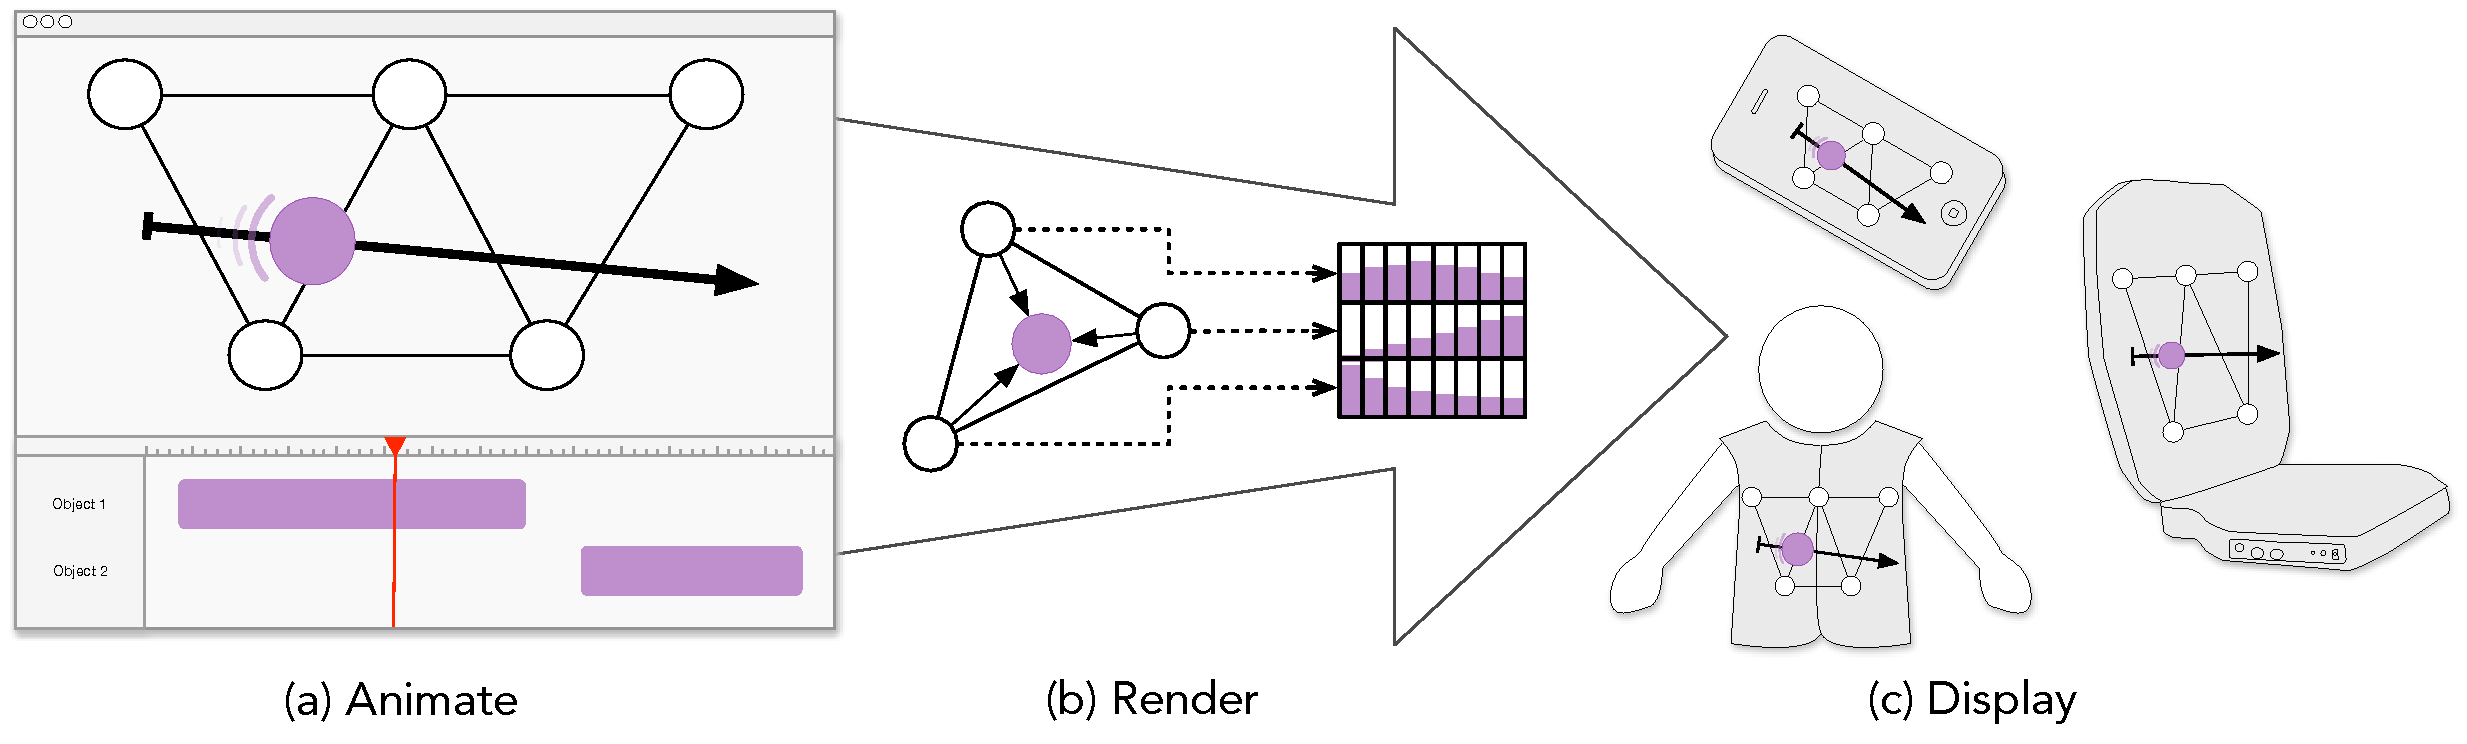
\includegraphics[width=0.98\textwidth]{images/HA14-Concept-Sketch-2015-01-17-1127}
   \caption{Concept sketch for tactile animation. 
An artist draws an animated sequence in the user interface and the user experiences phantom 2D sensations in-between discrete actuator grids. 
%The animator controls phantom sensations directly, without needing to think in device terms, and designs expressive sensations for arbitrary vibrotactile arrays.
}
   \label{fig:concept:sketch}
\end{figure}
% }

  

%Chairs, wearables, and handhelds have become popular sites for spatial tactile display.
%Visual animators, 
%already expert in using time and space to portray motion, could readily transfer their skills to production of rich haptic sensations if given the right tools.
In this second case study, we iterate on some of our findings from the haptic instrument to design a full authoring tool, using real-time feedback but supporting refinement with time-based editing.
This work\footnote{In peer review at the time of this writing.} targeted professional media designers (especially animators) creating spatial vibrotactile sensations.
To afford real-time manipulation, we developed the \emph{tactile animation object}, a persistent, manipulable primitive rendered through phantom vibrotactile sensations, and implement Mango, an editing tool built for animators.
%We describe Mango's interface, rendering pipeline, and perceptually-optimized interpolation algorithm.
In our evaluation,
professional animators found it easy to create a variety of
vibrotactile patterns, with both experts and novices preferring the tactile animation object over
controlling actuators individually.
Furthermore, the tactile animation metaphor is a generalizable concept that can extend to several devices.
%, which we explore before concluding.
%in authoring real-time feedback on a variety of grid displays.

  

  
%%%%%%%%%%%%%%
%
% Section - Intro
%
%%%%%%%%%%%%%%
%\section{Introduction}

%Haptic feedback is % increasingly 
%viewed in today's entertainment and media industry as a key ingredient of immersive experience.
%%%whose potential has not been unlocked.
%Motion platforms and large shakers appear in theater seats, ride vehicles, and gaming platforms to tilt, rotate, translate and shake the user's body to build engagement and fun.
%A new genre of haptic technologies aim to supplement movies, games, and even users' social activities with expressive and synchronized cues at multiple locations on the skin
%\cite{Israr2011,Danieau2012a,Sodhi2013,Kim2009}. 
%Similar opportunities await well-designed wearable and handheld displays.
%Unfortunately, adoption has been limited by the dearth of authoring tools for generating rich sensory content.
%
%
%%Critically, this haptic content is crafted, tested, synchronized and stored during media production using custom software plugins made for tools familiar to  media designers and artists,
%%requiring little modification to existing production pipelines. 
%%In this paper we present, implement, and evaluate key elements of a haptic authoring system that allows artists and designers to quickly generate spatio-temporal haptic media on multi-actuator haptic technologies. 
%
%Multi-actuator vibrotactile (VT) arrays,
%which stimulate the skin through vibration, appear in diverse applications and form factors, from chair-based immersive gaming  \cite{Israr2011} to wearable vests for mobile awareness \cite{Jones2004}.
%%To create expressive sensations, however, designers typically must be programmers and haptic experts.
%%Several device-specific tools for prototyping or final authoring of haptic sensations have introduced user-friendly and user-familiar interfaces. 
%Most VT authoring tools only support a single actuator \cite{Enriquez2003}; those that accommodate multiple actuators % deleted Lee2009
%control each separately \cite{Kim2009,Paneels2013,Swindells2014}.
%These multitrack authoring tools %allow designers to edit, test, and save time-series data for individual actuators, but
%are cumbersome and complicated for systems having as many as % greater than 
%%10 or 20 vibrating actuators (e.g., one haptic jacket for movie goers is equipped with 
%64 vibrators \cite{Jones2009}.
%%). %(Tactile 
%
%{\it Direct manipulation} of a spatial animation object provides
%%rather than by coordinating multiple tracks. 
%a simpler mental model that eases the transition of visual animators into haptic design.
%We build on the notion of a phantom vibration perceived in-between physical actuators \cite{Alles1970,Israr2011a} to support real-time spatiotemporal tactile feedback in sparse actuator arrays, enabling direct manipulation.
%Specifically, we present the %concept of a 
%\textbf{tactile animation object}, a visualized abstract phantom sensation, and implement it in \emph{Mango}, a tactile animation tool and rendering pipeline (\autoref{fig:concept:sketch}).
%
%
%Our contributions are: 
%%We have three contributions.
%1)  A tactile animation interface grounded in user interviews and prior literature.
%% The design is derived from interviews and prior literature, ..  includes tools 
%%Derived from interviews and prior literature, its design integrates techniques familiar to a mainstream animator workforce. 
%2) A rendering pipeline translating tactile animation objects %designed % animated 
%%haptic patterns to sparse VT arrays, and optimize its rendering algorithm with a user study.
%to phantom sensations on sparse, generalized VT arrays, optimized with a perceptual study.
%% We conduct a study to determine an optimal rendering algorithm for sparse VT arrays. 
%3) An evaluation with professional animators showing accessibility and expressivity.
%4) An exploration of the potential applications supported by tactile animation.
%% with \kmC{SLC} % in  ??? 
%%natural user gestures.
%% KM 04.12: at this point, 'animation metaphor' as connected to 'natural user gestures' is unclear - you haven't mentioned gestures yet so this comes out of nowhere. Can you restate this contribution more plainly?
%

\newcommand\prevWorkWidth{1in}
\newcommand\prevWorkImageWidth{0.65in}


%\begin{figure}[b]
% \centering
%   \begin{subfigure}[t]{\prevWorkWidth}
%	  \centering
%	   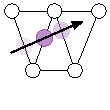
\includegraphics[width=\prevWorkImageWidth]{HA14-PreviousWork-TactileBrush-2015-04-12-1100} 
%	   \caption{Tactile Brush \cite{Israr2011a}: precomputed curves}
%	   \label{fig:prevwork:tactilebrush}
%    \end{subfigure}
%    ~
%  \begin{subfigure}[t]{\prevWorkWidth}
%  	\centering
%	   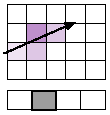
\includegraphics[width=\prevWorkImageWidth]{HA14-PreviousWork-TactileMovies-2015-04-12-1100} 
%	   \caption{Tactile Video \cite{Kim2009}: frames of tactile pixels}
%	   \label{fig:prevwork:tactilemovies}
%    \end{subfigure}
%    ~
%      \begin{subfigure}[t]{\prevWorkWidth}
%	      \centering
%	   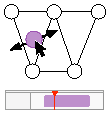
\includegraphics[width=\prevWorkImageWidth]{HA14-PreviousWork-HA-2015-04-12-1100} 
%	   \caption{Tactile Animation: direct manipulation}
%	   \label{fig:prevwork:ha}
%    \end{subfigure}
%    \caption{Comparison between related systems.}
%    \label{fig:prevwork}
%\end{figure}




%\begin{table*}
%	\begin{tabular}{|l|p{0.92\textwidth}|}
%	\hline
%	\rowcolor{tableheadercolor}
%
%	\textbf{LR}
%		%& \textbf{RW}
%		& \textbf{Description} \\
%	\hline
%		LR1 
%		 &
%		 \textbf{Real-Time Playback} \cite{Moussette2011,Schneider2014}
%		 Rapid prototyping is essential for working with VT sensations, especially in absence of objective metrics. % of success.
%		 Feeling a sensation at design time allows iteration to converge faster to better results. % and develop more engaging sensations.
%		 However, \textit{too} real-time can cause split attention.
%	\\
%	\hline
%		LR2 & 
%		 \textbf{Load, save, manipulate}
%		 \cite{Resnick2008,Johnson2002,Schneider2014}
%		 	A persistent object model is essential for sensation editing over % for being able to continue to work on sensations for 
%			longer projects and % for being able to share them 
%			sharing with other designers or across devices.
%			Well-defined actions upon a data structure also facilitates features like \textit{undo} that support experimentation.
%	\\
%	\hline
%		LR3 &
%		\textbf{Library of effects} \cite{Enriquez2003,Swindells2006,Herring2009,Paneels2013,Swindells2014}
%		% deleted Paneels2010
%			 A library of saved sensations is an important feature used in previous haptic authoring tools, providing inspiration and preventing designers from re-inventing the wheel.
%	\\
%	\hline
%		LR4 &
%		\textbf{Device configuration} \cite{Kim2009,Paneels2013,Lee2012,Lee2013}% deleted Lee2009
%			~Because of the many types of haptic devices, a general tool must be able to understand different devices.
%			Lightweight configuration files that describe each device are common in the literature.
%			The configuration file allows users to select specific hardware and specify location and type of actuators.
%			Animators can also select a rendering algorithm from a list of available ones.
%	\\
%	\hline
%		LR5 &
%		\textbf{Multiple channels \& combination of effects}
%		 \cite{Enriquez2003,Swindells2006,Ryu2008,Paneels2013,Swindells2014}	 
%		 Being able to display multiple effects simultaneously, or combine effects via superposition or concatenation, is essential for expanding the design space.
%		 This is typically represented in a timeline, which represents the temporal behaviour of any objects.
%	\\
%	\hline
%		LR6 &
%		\textbf{Visual/direct control metaphor}
%		\cite{Kim2009,Paneels2013,Cuartielles2012}
%		 Most previous tools consider each actuator separately.
%		 When thinking semantically about a spatial system, a direct view of the device and actuator layout is critical for direct manipulation.
%	\\
%	\hline
%		LR7 &
%		\textbf{Audio/visual context}
%		\cite{Kim2009,Swindells2014,Moussette2011}
%		 Haptic perception depends greatly on additional senses \cite{Hayward2008}. %cite hayward or pseudohaptics
%		By providing audio and visual feedback, these effects can be mitigated and the designer can experience haptic sensations in context.
%	\\
%	\hline
%		LR8 &
%		\textbf{User Feedback}
%		 \cite{Schneider2014,Swindells2014}
%		 Receiving feedback from users, either by demonstration or A/B testing, is extremely valuable.
%	\\
%	
%
%	\hline
%	\end{tabular}
%	\caption{{\bf Literature Requirements (LRs)} for a tactile animation authoring  tool.}
%	\label{tab:design:literature:requirements}
%\end{table*}



%%%%%%%%%%%%%%
%
% Section - Requirements Gathering
%
%%%%%%%%%%%%%%
\section{Mango, a Tactile Animation Authoring Tool}
% The objective of the haptic authoring tool 
To create a familiar and efficient % authoring
framework for  dynamic haptic content, we gathered two sets of requirements: Literature  (``LRs"), from prior research on haptic authoring tools, and Industry (``IRs") from interviews with five industry experts in haptic media creation and animation.
Our prototype, Mango, was built in  Python 2.7 and Tkinter (\autoref{fig:implementation:screenshot}),
communicating with a devices via USB.




%%%%%%%%%%%%%%
%
% Section - Framework
%
%%%%%%%%%%%%%%

%\subsection{Framework for Tactile Animation}
%%%%%%%%%%%%%%
%
% Framework for Haptic Animation


%In this section, we present an animation metaphor that allows users to generate tactile content in the same way as they would create visual animations and play them real-time on a VT array.
%\autoref{fig:feel:taxonomy} shows the workflow of this authoring mechanism.  
Designers create tactile animations on Mango as they would in a graphical animation tool. % as shown in \autoref{fig:feel:taxonomy}a.
The animation object is placed in space, and the designer adjusts % at a location and designers adjust 
its size on the visual outline of the VT array. %\kmC{SLC}. % KM 04.12: 'trace of a VT array" is unclear to me. 
% Once the object is created, they 
The designer then adds movements and special effects to the object using Mango's toolset,
% a set of tools provided in the Mango interface, 
and play it to observe timing. % of the animation. 

Mango's rendering engine translates visual animations to tactile animations on the VT array
%Knowing the location of vibrating points on the coarse array of VT actuators, the rendering engine resolves the animated sequence into individual actuators using the phenomena of phantom tactile sensations \cite{Alles1970,Israr2011a}. 
%The phantom sensation is a sensory illusion elicited by stimulating two or more vibratory elements on the skin.
%Instead of feeling the individual vibration points, the user feels a single sensation in between, whose perceived intensity is defined by the weighted sum of the intensities of the vibrating elements.
%Therefore, in each frame, the animated tactile object is resolved into intensity of actuators on the VT array (\autoref{fig:feel:taxonomy}b) .
%The rendering engine then calculates raw waveforms for each VT channel (\autoref{fig:feel:taxonomy}c) that can either be sent to the VT device to play the animated sequence or exported as a multichannel datafile for later use.
%Previous work has interpolated between only two actuators \cite{Seo2010,Lee2012a}; % KM 04.12 missing ref?
%however, a more generalized 3-actuator interpolation algorithm allows for arbitrary real-time manipulation of the tactile animation object on grid displays. 
%, but is less understood perceptually. As such, we guide our rendering algorithm with a perceptual study.
% presents additional challenges, including choosing a suitable rendering function
%OS: Should we explain that previous work has only interpolated between two actuators? Or would that invite questions about whether it feels right?
% KM: I think you risk this coming up if you don't.
%
% COMMENTED OUT JAN16 2:30PM PST
%
% all chan
%
%Several methods
%
%called \emph{vector sensations} (\autoref{fig:feel:taxonomy}(b)), 
%
%and each vector represents variation in intensity of the corresponding actuator of the VT array. From these vector sensations, the rendering engine calculates the raw waveform, called \emph{raster sensation}, at each sample instant for haptic rendering (\autoref{fig:feel:taxonomy}(c)). The sample rate for haptic rendering is usually faster than the frame rate and raster sensations are combination of intensity variations (vector sensations) and the stimulation frequency. These raster sensations are then sent to the haptic devices (\autoref{fig:feel:taxonomy}(d)) t
%To accommodate the animation framework, we define
using three {\bf datatype models}:
%for use in the current implementation and  future expansion of the Mango tool:
% if tight on space, following sentence is redundant with remainder of section since full refs are on same page.
\emph{Tactile animation objects}, high-level hardware-independent data types for tactile animation;
\emph{vector formats}, high-level hardware-specific control common in previous work; and
\emph{raster formats}, low-level hardware-specific formats for rendering and playback.
Data types are stored as JavaScript Object Notation (JSON) files.

%\textbf{Tactile animation objects} % KM: could save sig space by defining acronomym, given # of appearances.
%are high-level specifications of virtual sensations moving on a 2D VT array (\autoref{fig:feel:taxonomy}a).  
%High-level parameters, such as location, size, and other semantic qualities, can either be constant or variable. % interpolation methods. 
%Each tactile object has a start time and a duration.
%Object type is also defined for tactile animations that sets pre-defined parameters and features to animated objects. 
%For example, a moving virtual point can have a position, size, and frequency parameter; while a ``rain" effect has a position and more semantic parameters like raindrop frequency or size.
%
%%Similarly to visual effects present in animation tools like Adobe After Effects, each animation type is pre-programmed with various parameters and shown as tracks in timeline.
%%The detailed implementation of different animation object types is left for future expansion of Mango.
%
%Tactile animation objects are device-independent.
%Mango uses a device configuration file (LR4) and the rendering engine to create animated VT patterns on hardware.
%Animation objects can be combined in novel ways, organized in groups, or generate other tactile animations like a particle generator as in a graphical animation tool, and can have paths that constrain motion to a pre-determined trajectory.
%We prototyped an early version of the tactile animation object in Mango; however, the data type is extensible.% for future expansion. 
%

\begin{figure}[tbh] %  figure placement: here, top, bottom, or page
   \centering
   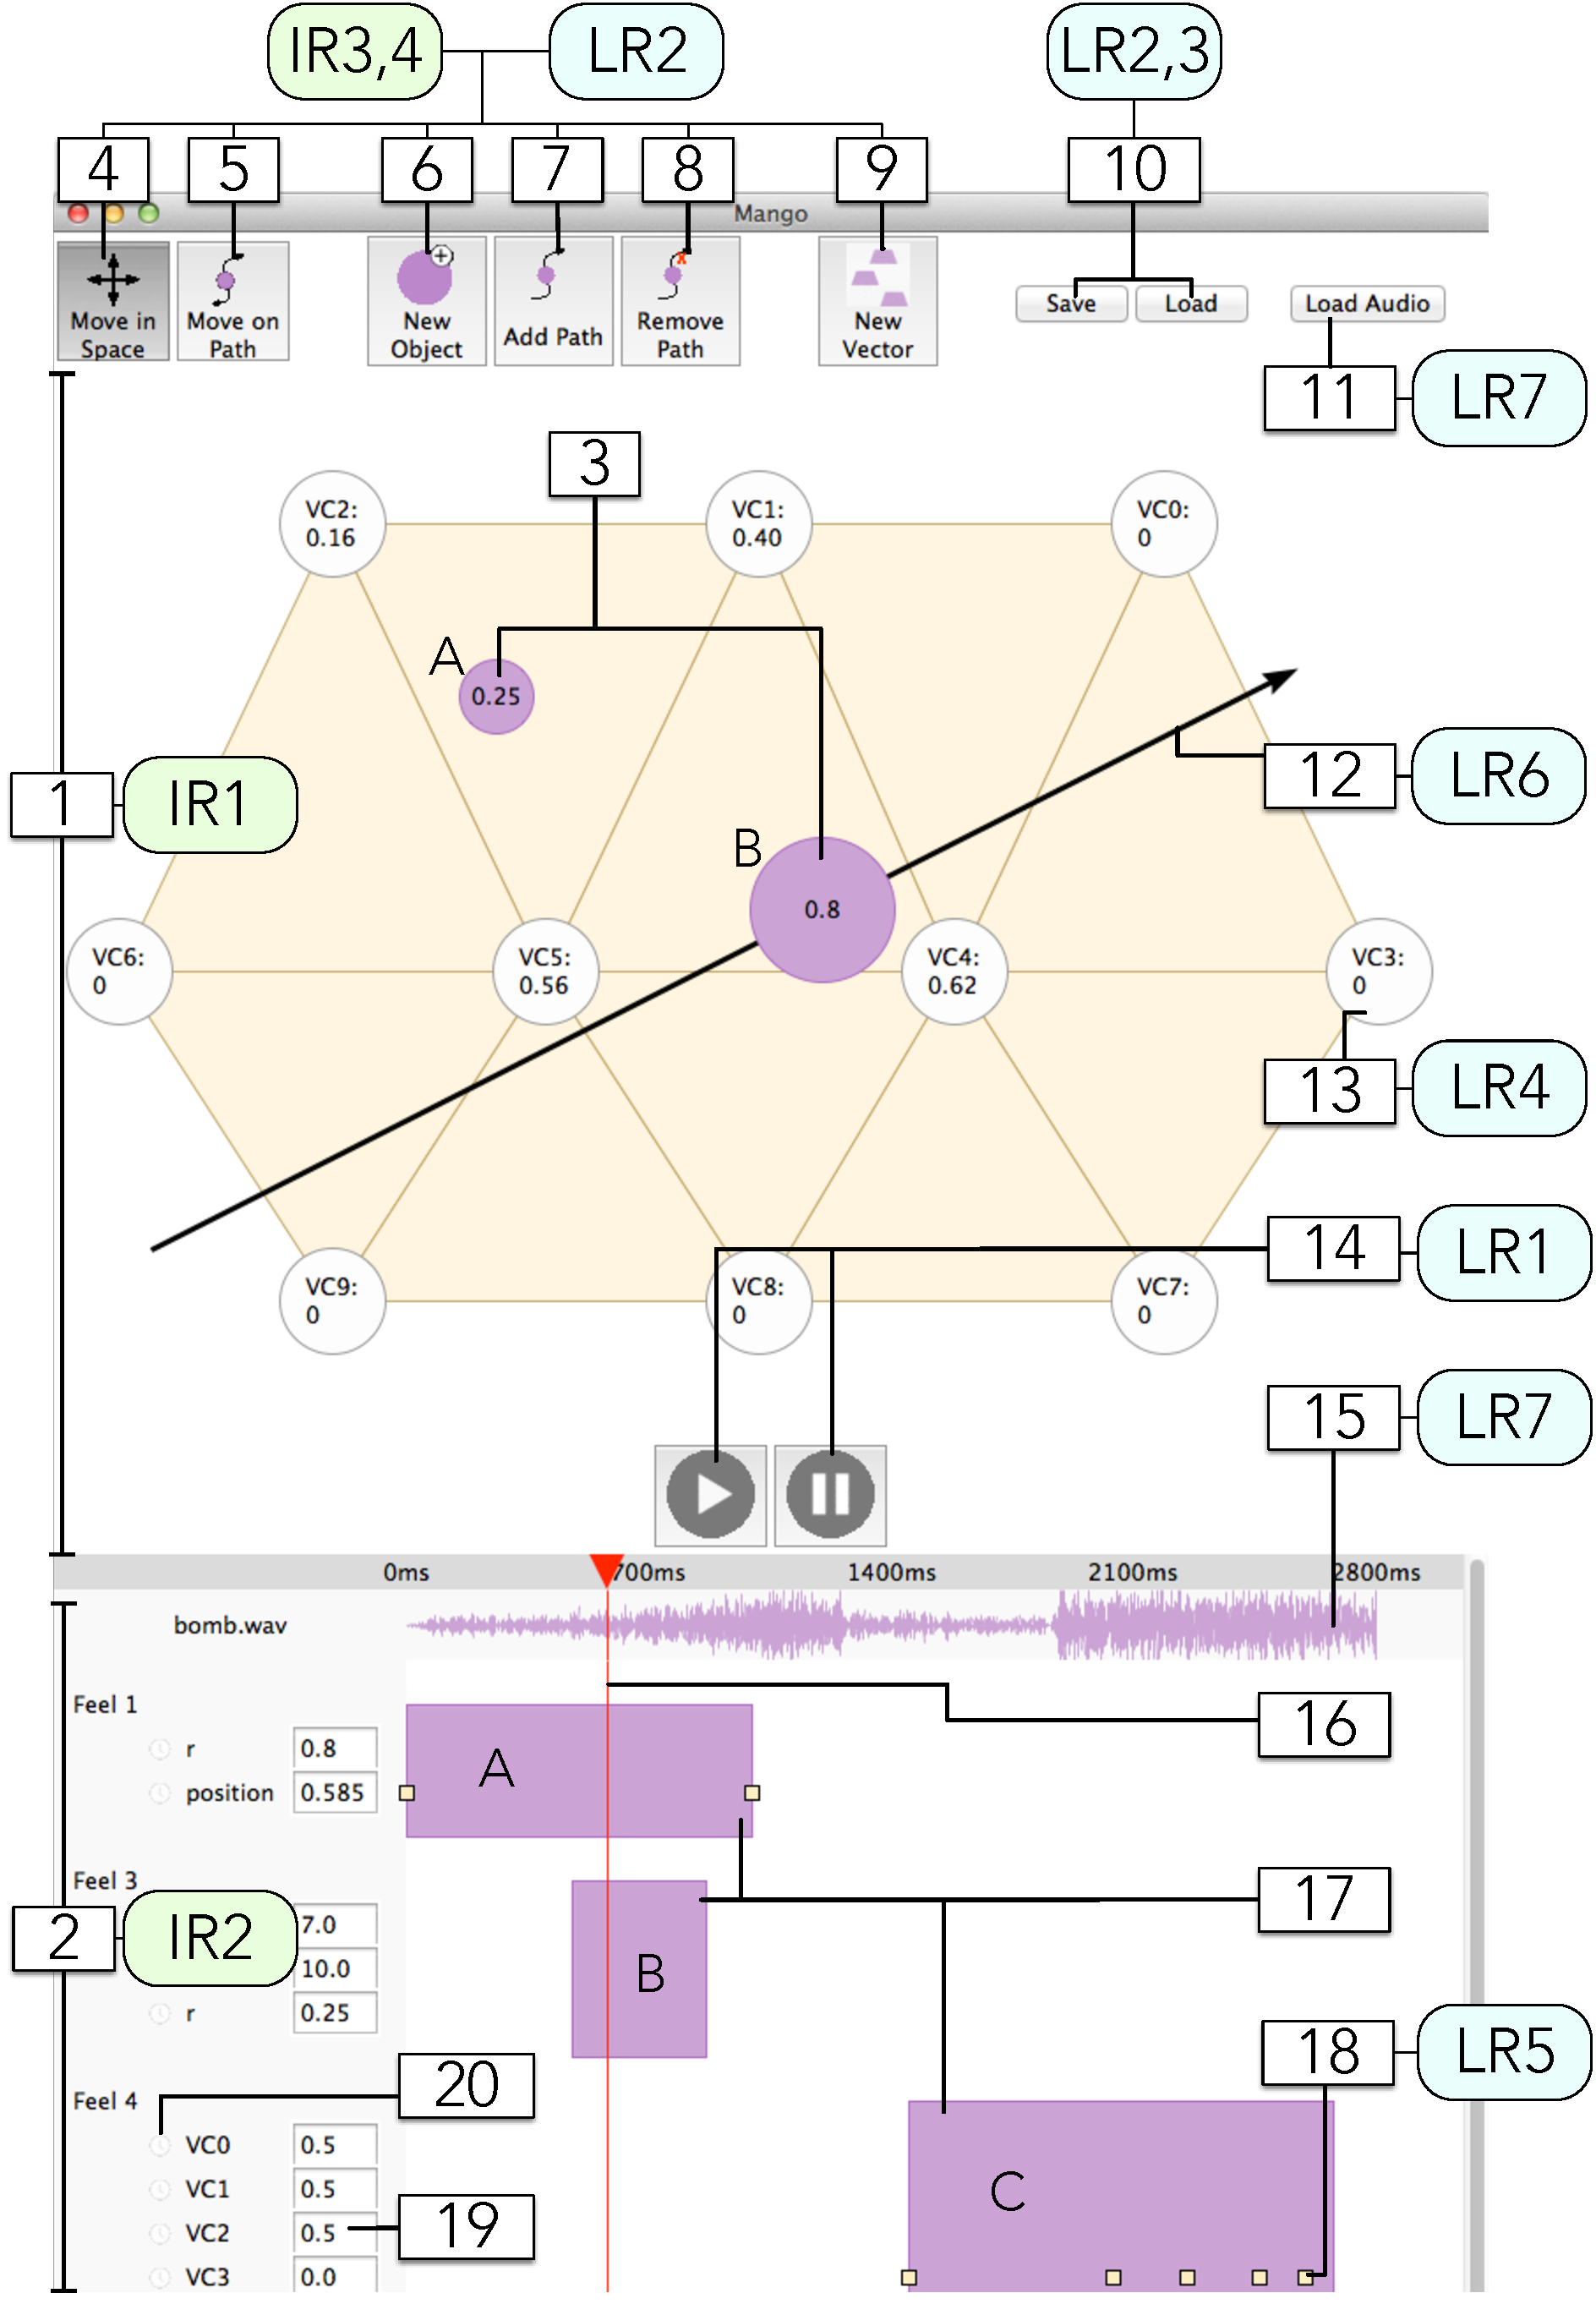
\includegraphics[width=0.47\textwidth]{Mango-Screenshot-Labeled-2015-04-12-1132} 
   \caption{Mango graphical user interface. Key components are labeled and linked to corresponding design requirements (LRs and IRs, not described in this proposal).}
   \label{fig:implementation:screenshot}
\end{figure}


%%%%%%%%%%%%%%%
%%
%% Section - Design
%%
%%%%%%%%%%%%%%%
%\subsection{Authoring Interface}
%%%\ALIc we need a good introductory sentense for this section.
%The authoring interface % is the key component in the Mango tool and % KM: so is the rendering pipeline isn't it?
%allows designers to efficiently create moving tactile content in a familiar environment.
%Here we describe user interactions to generate animated tactile content and associate them with our gathered design requirements. 
%% gathered in Section 3. 
%% In Mango's implementation, 
%Most Mango interactions are through the animation window (1) and  timeline (2) .
%%


%%%%%%%%%%%%%%
%
% Rendering Pipeline
%
%%%%%%%%%%%%%%
\section{Rendering Algorithm}
Mango's rendering algorithm translates animations in the animation window to animated VT patterns on the hardware.
%\autoref{fig:feel:taxonomy} shows the rendering pipeline that converts animation objects to vector sensations and a raster format, which outputs to the hardware.
The rendering algorithm
%is derived from %deep and extensive \kmC{SLC} % KM 04.12: are you sure about "deep/extensive"? sounds funny to me.
%psychophysical understanding of VT illusions on the skin and creates percepts of virtual actuators and their motion in between a set of real actuators.
%The precise perceptual model depends on several factors, such as type of VT actuators (DC vs. voice coil motors), stimulation site (forearm vs. back) and the spacing of actuators in the array (e.g., \cite{Israr2011a}).
%To allow for custom framerates and real-time feedback, we
generalizes from 1D phantom sensations (between two VT actuators along a line \cite{Seo2010,Alles1970,Israr2011a}) to 2D (between 3 or more actuators, \autoref{fig:rendering:algorithm:barycentric}).
%Thorough investigation of the psychophysical model is beyond our present scope; however, we empirically determine 
%the most effective model among those  % optimal model that is derived from various methods
% documented in the literature for the 1D case.
 %\kmC{2D vs 1D, slc} % KM: don't you need to go into more detail on 2D vs 1D? this seems like it's hinting at something without saying it.
%
%Here we describe the interpolation models for rendering algorithm used in the prior literature, and a pairwise comparison user study to determined the optimal interpolation model for the Mango's rendering algorithm.

%\subsection{Algorithm}
%The rendering algorithm translates virtual percepts to a physical actuator grid.
%We first construct a Delaunay triangulation for all actuators to automatically define a mesh on the hardware grid.
%At each instant of rendering, we use barycentric coordinates of the virtual animation objects relative to a triangle defined by three real actuators (\autoref{fig:rendering:algorithm:barycentric}).
%Barycentric coordinates are scaled by an interpolation method to determine real actuator intensity.
We had to choose between three interpolation models from prior psychophysical understanding of phantom tactile sensations \cite{Alles1970} and propose them as candidates for the Mango tool:
% They are: 
(i) {\it linear}, 
(ii) {\it logarithmic (``log")}, and 
(iii) {\it Pacinian power (``power")} interpolation. 
%
%%In the linear interpolation model, barycentric coordinates are linearly related to actuation amplitude. In the log model, these coordinates are scaled logarithmically, as perceived intensity is related to physical vibration amplitude 
%%\cite{verrillo1992perception}. In the power model,  coordinates are coupled to the power (square of the amplitude) of vibrating stimulations \cite{verrillo1992perception}. 
%%Linear and log interpolation models have been used in the past to express either location or intensity respectively (but not both) of virtual sensations between two vibrators \cite{Seo2010,Alles1970}. A Pacinian power model was used in \cite{Israr2011a} to account for both location and intensity of virtual sensation between two vibrators.
%

\begin{figure}[t] %  figure placement: here, top, bottom, or page
   \centering
  \begin{subfigure}[b]{0.4\textwidth}
  	\centering
	   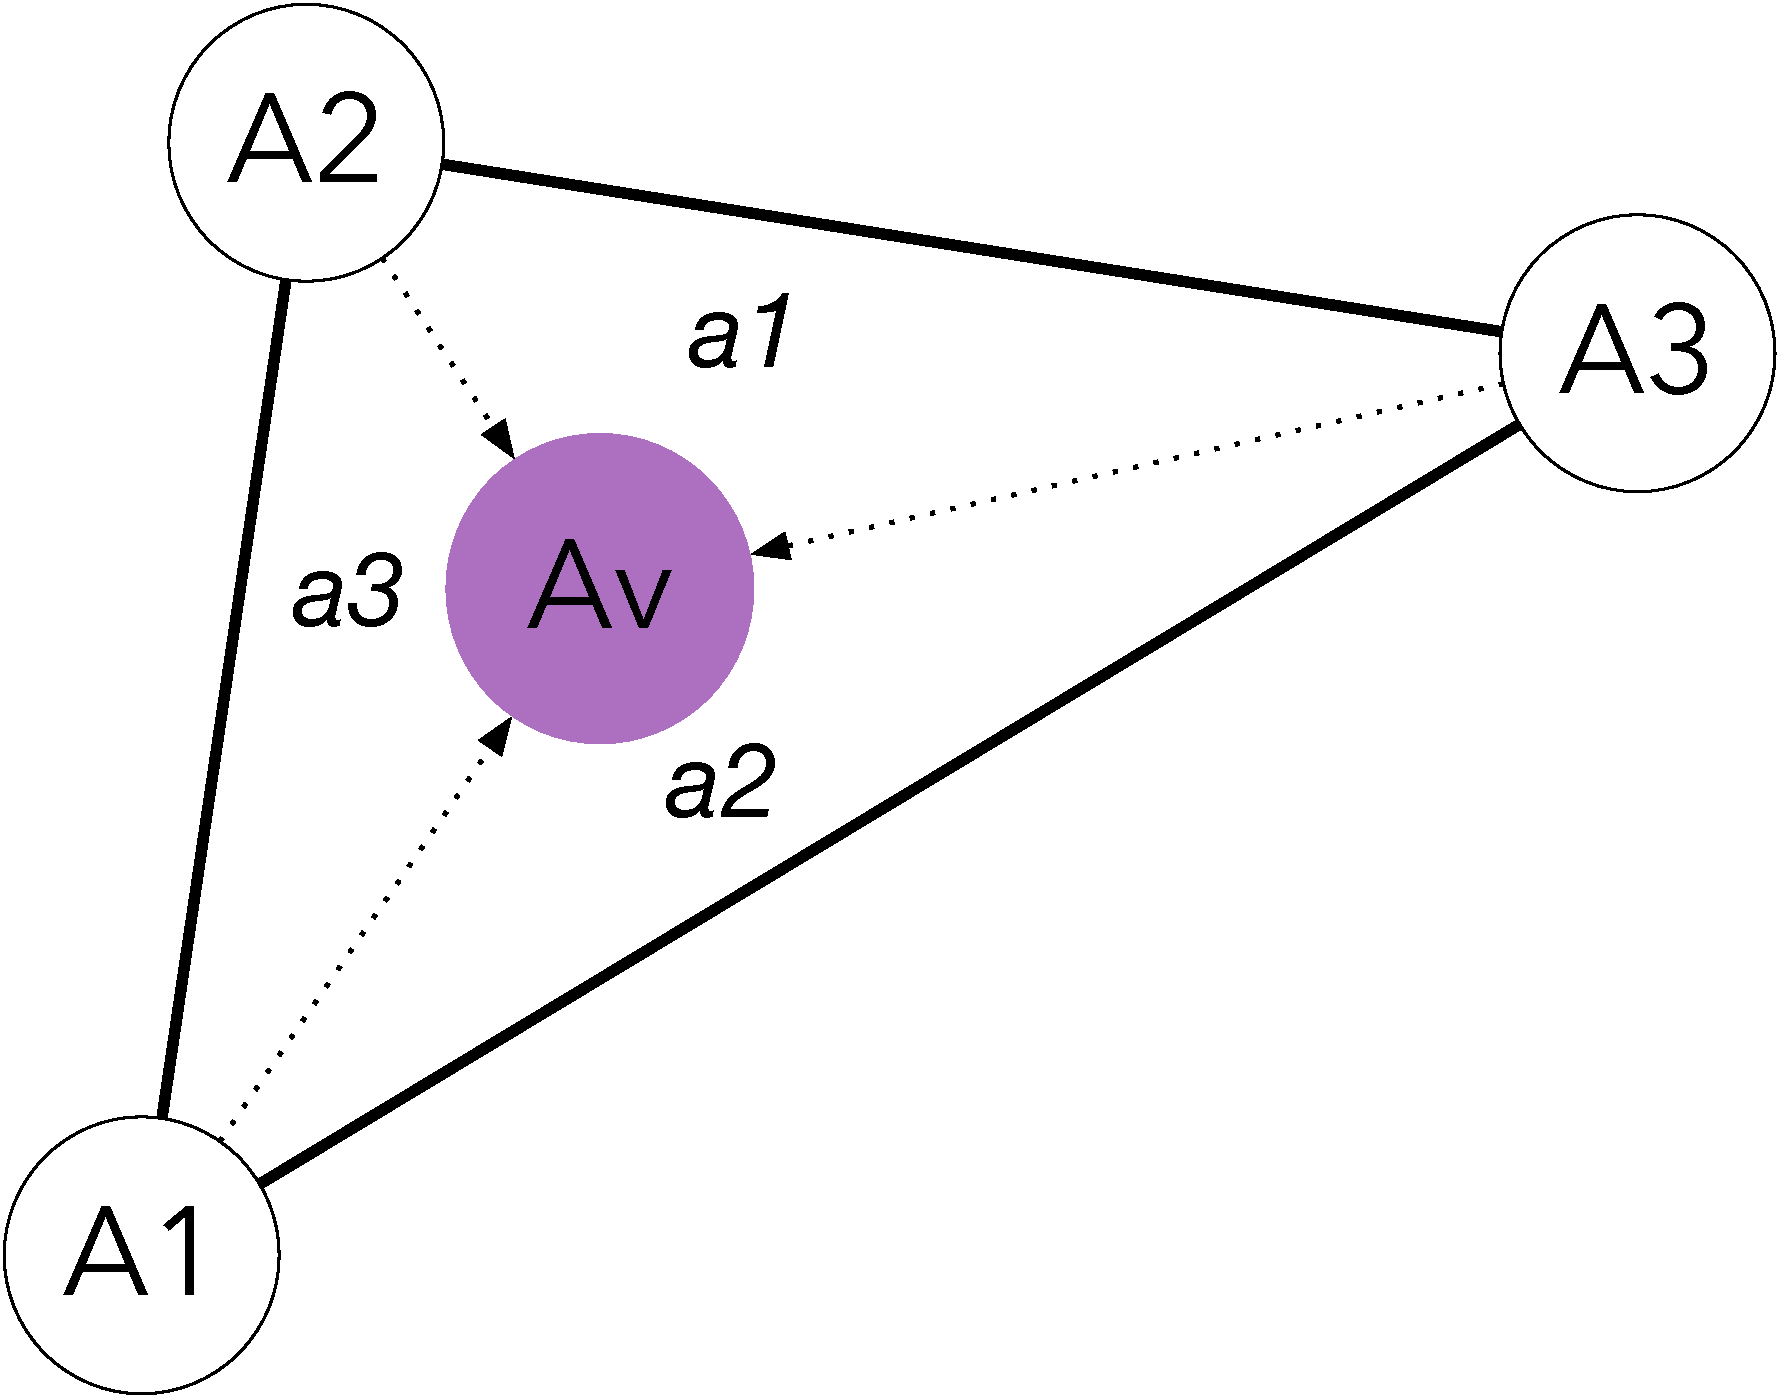
\includegraphics[width=0.8\textwidth, height=1.5in]{HA14-RenderingFigure-2015-01-17-2129} 
	   \caption{Barycentric coordinates.}
	   \label{fig:rendering:algorithm:barycentric}
    \end{subfigure}
    \qquad
     \begin{subfigure}[b]{0.4\textwidth}
       	\centering
	   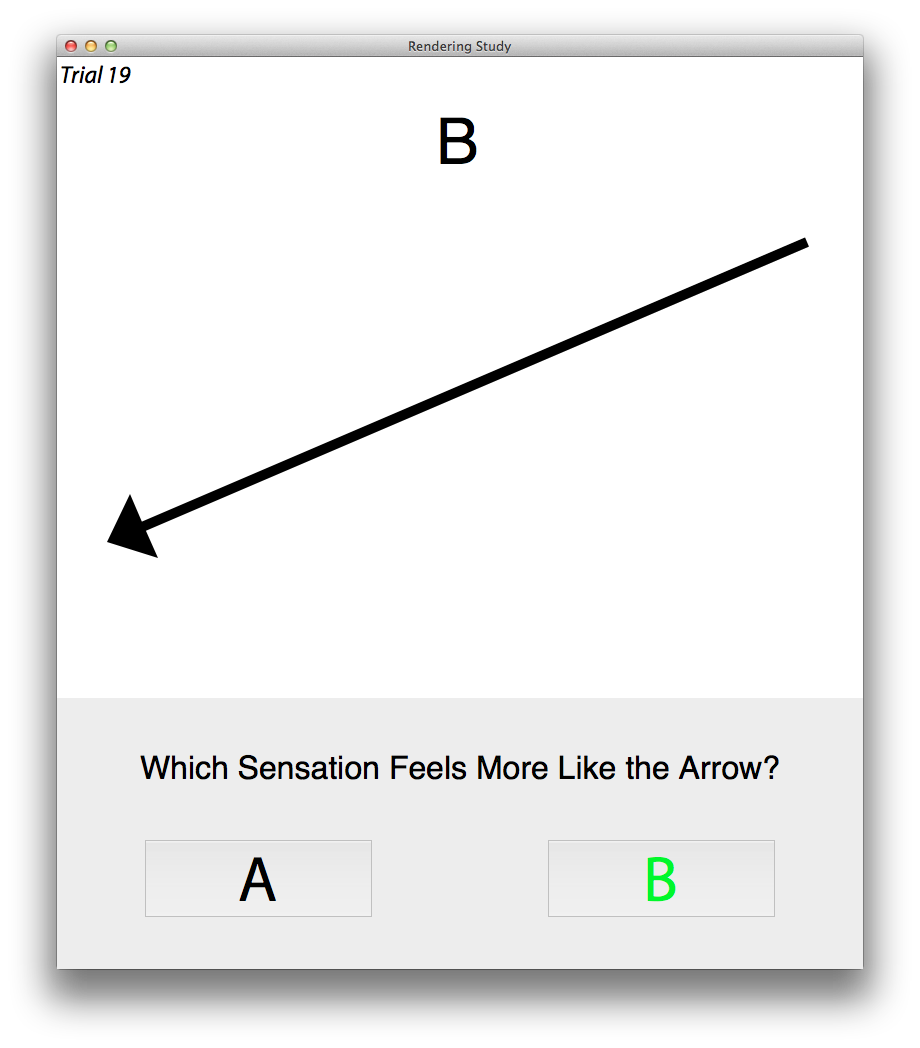
\includegraphics[width=0.6\textwidth, height=1.5in]{HA14-RenderingUI-2014-08-19-1417} 
	   \caption{Rendering study interface}
	   \label{fig:rendering:study}
    \end{subfigure}

    	   \caption{We ran a study to determine the preferred interpolation function to map barycentric coordinates (a1-3) to physical actuator output (A1-3) given a virtual intensity (Av).}
	   \label{fig:rendering:algorithm}
\end{figure}
%
%
%
%%%%%%%%%%%
%%
%%
%%
%%\subsection{Perceptual Study}
%
% Our first study is 
%We performed a pairwise comparison between the three candidate interpolation models prototyped for Mango's rendering pipeline.
%Our goal was to determine the user-preferred model for this VT hardware, to be used in Mango's ongoing implementation; and to identify relevant factors (e.g., frequency, amplitude, or individual differences).
%To determine the preferred model for this VT hardware in Mango's rendering pipeline, and to identify relevant factors (e.g., frequency, amplitude),%, or individual differences), 
We performed a pairwise comparison of our three candidate interpolation models.
Eighteen volunteers took part (6 female, between age 20-35). % aged 21 to 34) . 
%
%The VT hardware consisted of 10 high-quality VT actuators (C2 tactors, Engineering Acoustics, Inc., USA) arranged in a 3-4-3 layout and mounted on the back of a chair in a pad  21 cm high, 29 cm wide, and 2 cm thick;  actuators form equilateral triangles with edges of 6.35 cm  (\autoref{fig:rendering:device}). %The rendering engine updates at 100 Hz.
%\subsection{Results}
Analysis with stepwise regression revealed that logarithmic interpolation outperformed linear and was % found 
equivalent to Pacinian power model. We proceeded with the logarithmic model for Mango's implementation, as the power model did not outperform either of the others. % the linear model.
%Through piloting, we determined that the device's on-screen visual outline should mirror the sensations rendered on the physical device. That is, if participants see an animation object on the right side of the screen, they prefer to feel it on the right side of the back. 
% (as if they are looking from behind the VT hardware). 
\autoref{fig:rendering:study} shows the experiment interface, in which an arrow represents the sensation direction. 


\begin{figure}[t] %  figure placement: here, top, bottom, or page
   \centering
     \begin{subfigure}[b]{0.43\textwidth}
	   	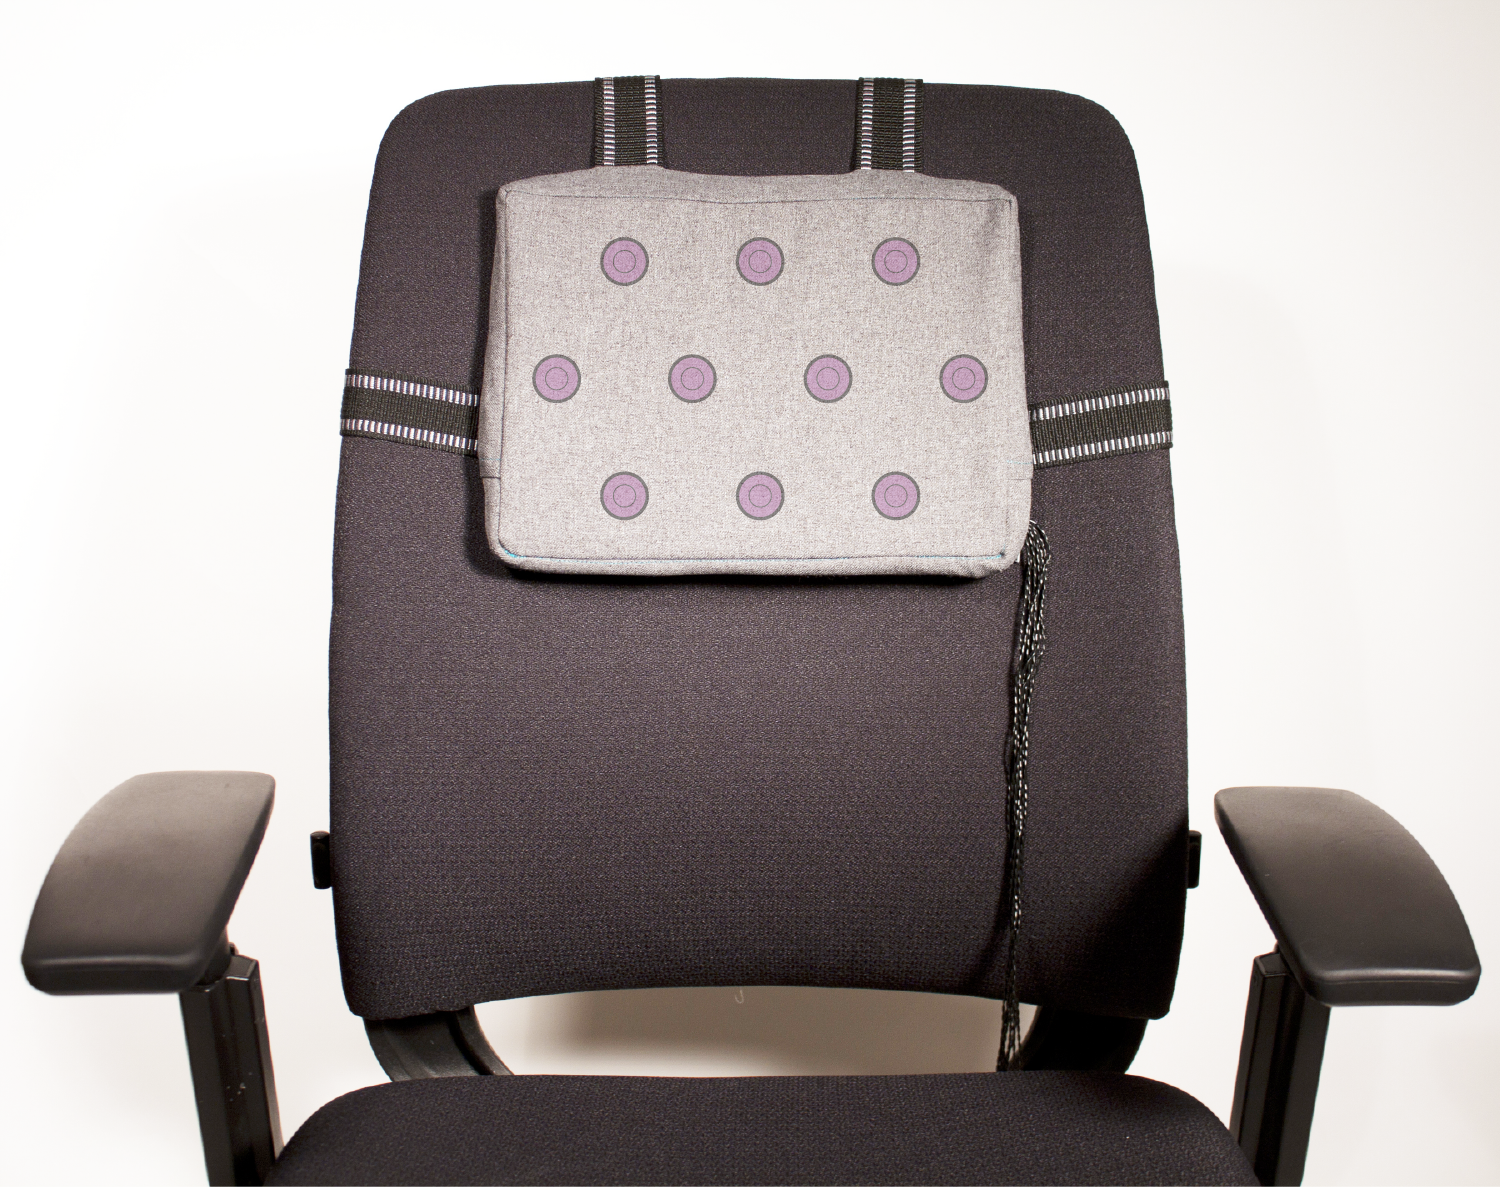
\includegraphics[width=\textwidth]{figure_chairpad} 
	   \caption{Output device with highlighted actuators}
	   \label{fig:rendering:device}
    \end{subfigure}
    \qquad
       \begin{subfigure}[b]{0.5\textwidth}
       		\centering
	   	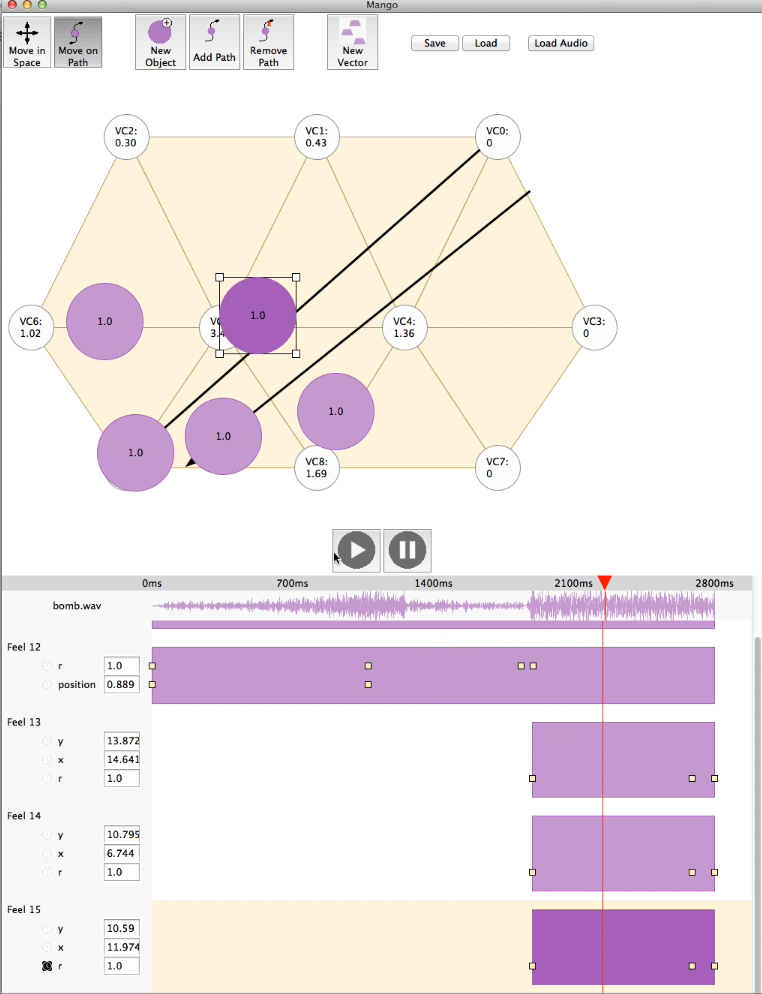
\includegraphics[clip=true, trim= 4 175 0 85, width=0.8\textwidth]{P2_sound_example-2014-09-22-1630} 
	\caption{Example of P2's animation for matching a sound.}
	\label{fig:animation:example:p2}
    \end{subfigure}
    	   \caption{Evaluation study setup and example design.}
	   \label{fig:rendering}
\end{figure}



%%%%%%%%%%
%
% Animation Tool Evaluation
%
\section{Design Evaluation}
% We implemented the critical functional features of Mango as described in the above sections.
To evaluate Mango's % the 
animation metaphor and expressive space with critical functional features implemented, we asked media professionals to
% we had media professionals 
create a variety of designs.
%, and qualitatively evaluated 
%its use for creating haptic content using both tactile animation objects (current design) and vector sensations (the state-of-the-art approach). 
%
%\subsection{Protocol}
Six participants (P1-6, 3 females) were introduced to Mango driving % linked to 
the  VT hardware described for the pairwise comparisons. 
%P1 had experience with haptics but not animation beyond video editing;
%P2-5 had animation experience but little or no experience with haptics;
%P6 had no experience with haptics or animation, but was familiar with media tools like Adobe Photoshop.
%P5 was also involved with the requirement gathering interviews presented earlier.
Each entire session took 40 to 60 minutes and consistened of a training task then three design tasks: design a heartbeat sensation, a ``turn left" sensation, and a sensation that matched a sound.
A semi-structured interview followed the design tasks informed by phenomenological protocols \cite{Moustakas1994}.
%The interviewer then followed up on interesting statements and/or concerns.
%During the interviews, participants were asked to compare animation objects with vector sensations, and to walk through the interface to elicit feedback.
%
% Study 2 results
%
%\subsection{Results}
Results were analyzed
% by considering each statement, memoing, coding, and relating codes
according to % Corbin and Strauss's 
grounded theory methods \cite{Corbin2008}, creating four themes.

%Each participant was introduced to Mango with a training task: % and the use of tactile animation objects and vector sensations.
%designing an alerting sensation using %  ``alert" sensation with 
%either animation objects or vector sensations (order counterbalanced).
%%half of them used the animation objects first and the other half used vector sensations first.
%Then, each participant was given three design tasks.
%1) Primarily \emph{temporal}: create a heartbeat sensation.
%2) Primarily \emph{spatial}: tell a driver to turn left.
%3) \emph{Context-based}: create a tactile animation to match a sound file.
%A 3-second sound effect of a bomb falling (with a whistle descending in pitch) then exploding with a boom was chosen, i.e., complex with with two semantic components.
%The wide array of resulting designs can be found in the accompanying video.
%

%
% Show one animation
%
%\begin{figure}[ht] %  figure placement: here, top, bottom, or page
%   \centering
%%   	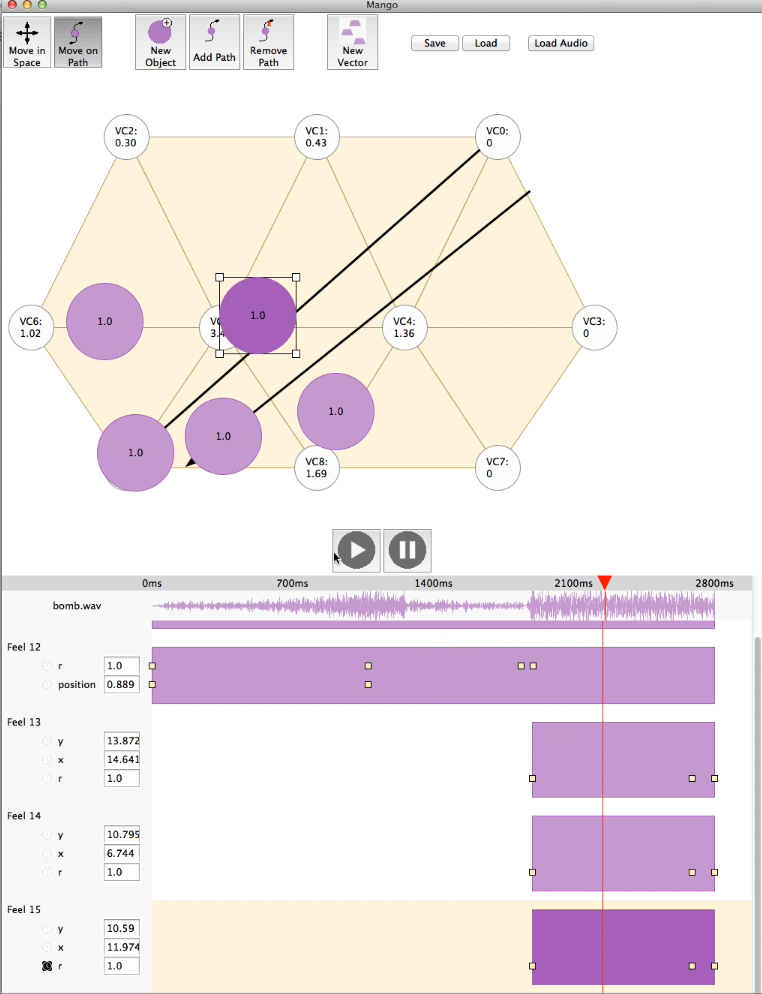
\includegraphics[clip=true, trim= 1 150 0 7, width=0.4\textwidth]{P2_sound_example-2014-09-22-1630} 
%	   	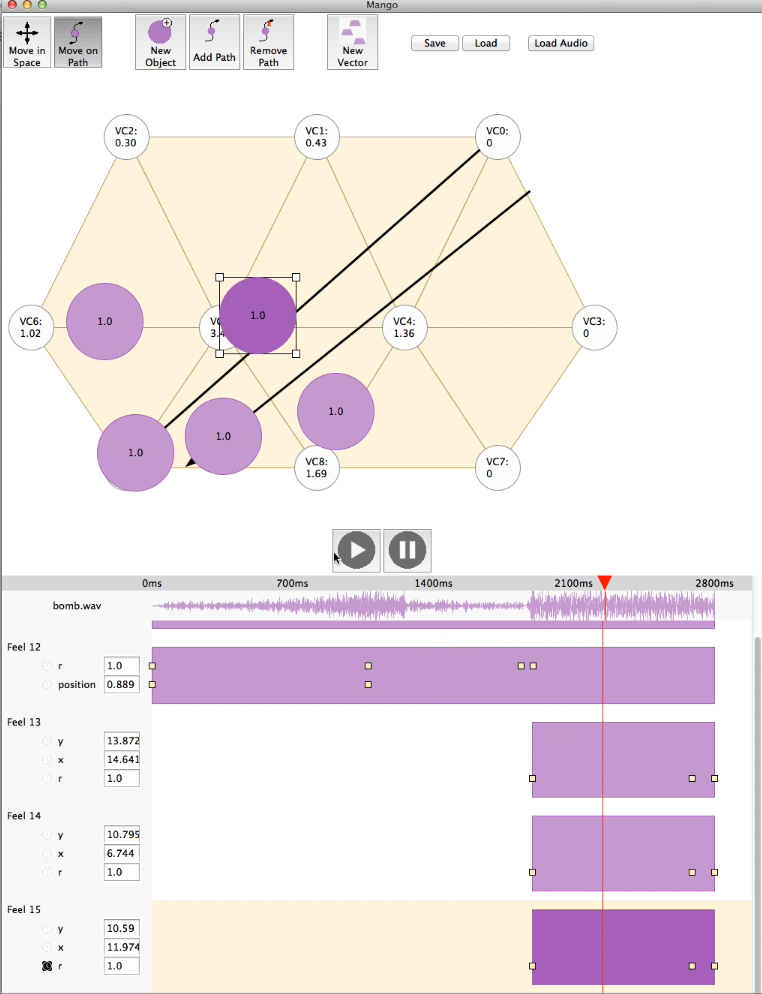
\includegraphics[clip=true, trim= 4 155 0 85, width=0.55\textwidth]{P2_sound_example-2014-09-22-1630} 
%
%	\caption{Example of P2's animation for matching a sound.}
%	\label{fig:animation:example:p2}
%\end{figure}




\textbf{Theme 1 - Animation Metaphor}
Participants found the tool easy to use.
All six participants were able to accomplish all five tasks (object alert, vector alert, heartbeat, turn left, sound) within their session.
%and described the interface as intuitive (P1-5), agreeing that it was an animation tool: \qq{It's up to the standards of other animation tools}{P1}, \qq{This is totally animation}{P2}, \qq{It felt very much like an animation tool}{P4}, \qq{I'm not an expert when it comes to haptics, but this software seems almost as if it can change the game of designing haptic vibrations}{P5}.
Negative feedback focused on polish and feature completeness.
%% not implementing enough features of their preferred tools and general feedback on polish and streamlining of the interface:
%\qq{gotta spline [the keyframe interpolation]}{P2}, \qq{a couple quirks but there was nothing difficult to overcome}{P4}, \qq{being able to design your own curve [path] would be really nice}{P5}, \qq{move in space and move on path can be one thing}{P6}.

\textbf{Theme 2 - Tactile Animation Object vs Vector Sensations}
Participants relied more on animation objects %  used animation objects more frequently
than vector sensations. %, which
%Vector sensations 
%were only used twice.%: P4's heartbeat task and P5's sound task (combined with an animation object).
%P1 switched from vectors to animation objects early in her heartbeat task;
%for her remaining tasks
%no other participants used vector sensations.
Animation objects were described as easier to use and more intuitive, especially to represent location or for non-animators.
%\qq{After using the new object I'd probably never use new vector again}{P2}, 
%%especially to describe motion or position:
%\qq{easier to find the location of the heart}{P1}, 
%%They were also described as more appropriate for people without animation experience:
%\qq{if I weren't an animator I think I would only use [animation objects]}{P4}.
%%, \qq{You have to be a little more careful when animating [vector sensations]}{P5}.
%%
%%Animation objects and vector sensations supported different workflows. Animation objects tended to be described as better for position, movement, and for % if you wanted to have 
%%multiple objects, while 
Vectors were preferred for more fine-tuned control when motion didn't matter as much, often using many keyframes.
%\qq{You can control multiple [actuators] at the same time, so you don't have to create new objects and then put them everywhere on the screen}{P1},
%\qq{[Animation objects] can be more comfortable to use when one doesn't work with keyframes}{P3}, 
%\qq{If you want precise control over [actuators], then vector is the way to go}{P4}.
%Participants rarely combined the two:
%\qq{I'm already into the object mode, I forget about the vector}{P6}.

%
% Shows three animations
%
%\begin{figure*}[htbp] %  figure placement: here, top, bottom, or page
%   \centering
%      	\begin{subfigure}[b]{0.30\textwidth}
%		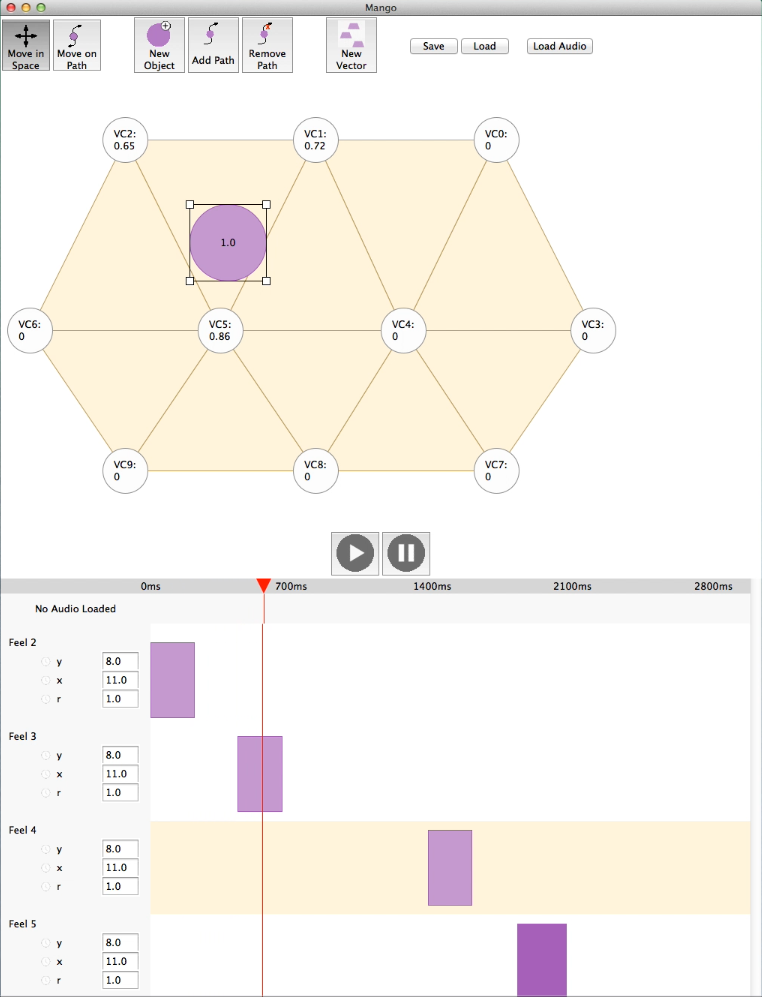
\includegraphics[width=\textwidth]{p1-heartbeat-example} 
%		\caption{Heartbeat task by P1}
%		\label{fig:animation:example:p1}
%	\end{subfigure}
%	\quad
%	\begin{subfigure}[b]{0.30\textwidth}
%		   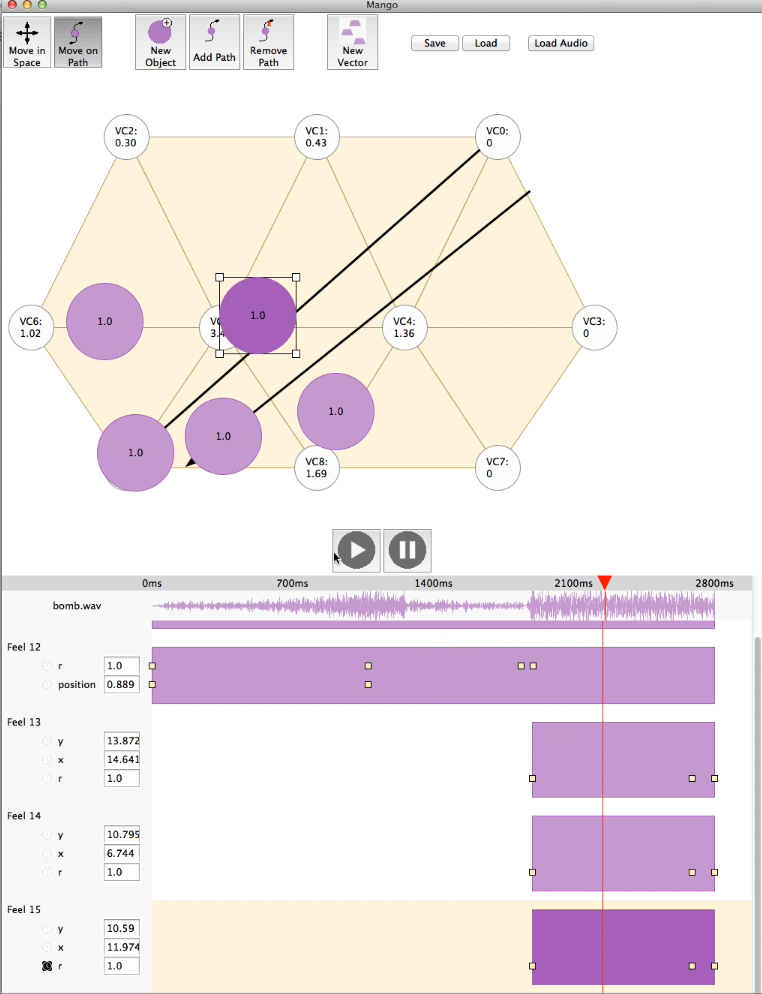
\includegraphics[width=\textwidth]{P2_sound_example-2014-09-22-1630} 
%		   \caption{Sound task by P2}
%		   \label{fig:animation:example:p2}
%	\end{subfigure}
%	\quad
%	\begin{subfigure}[b]{0.30\textwidth}
%		   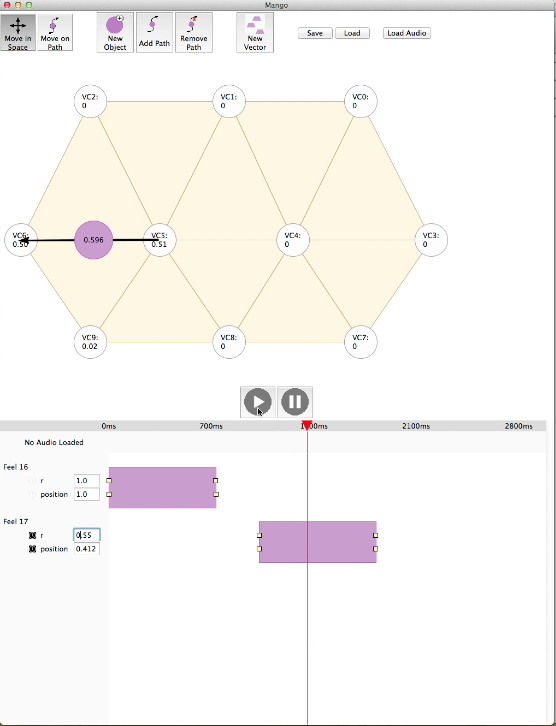
\includegraphics[width=\textwidth]{p4-turnleft-example-2015-01-19-1024} 
%		   \caption{Turn left task by P4}
%		   \label{fig:animation:example:p4}
%	\end{subfigure}
%
%
%
%
%      	\caption{Examples of Animations}
%	\label{fig:animation:example}
%\end{figure*}


%\theme{4}{Feedback, Context and Imitation}
%\theme{3}{Designing-in-action with direct manipulation}
\textbf{Theme 3 - Designing-in-action with direct manipulation}
Participants used direct manipulation to feel their designs in real time, %  was valuable to participants.
dragging animation objects %in the animation window
and scrubbing through
%at various speeds in
the timeline.
%: \qq{I would make the [animation] object and just play around with it before creating the animation, as a way to pre-visualize what I was going to do}{P5},
%\qq{I kind of play around with it, and randomly come up with the ideas}{P6}.
%P2 even noted that YouTube did not have
% real-time video scrubbing feedback like Mango's:
% %support for haptic and audio feedback:
% \qq{I wish I could scrub back and forth [with YouTube]}{P2}.
%However, continual % constant 
%vibrations were annoying, and participants requested a ``mute" feature:
%A VT feedback ``mute'' would be welcomed.
%P4 and P5 moved the timeline so that no output would play during design phase. 
% was playing while they were in design phase.
%\qq{It would be nice if when I [enter values into text fields] it doesn't go off constantly, it's getting annoying}{P3}.
%It was further suggested that each object should be independently mutable (as in hiding Photoshop layers), and VT output should be mutable entirely. 
More generally, participants used feedback from their experience or external examples.
P1 stopped to think about her heartbeat,  P2 used a YouTube video of a heartbeat as a reference, and P3 based her alert on her phone. %directly stated that she
%used imitation for the non-sound tasks
%;  her alert consisted of two vibrations similar to her phone: 
%\qq{It's typical to have two beeps for mobile phones}{P3}.
Similarly, participants were excited when prompted by an audio sensation.
%: \qq{I was really happy with the bomb one, because I could really hear it and imagine me watching a TV and then feel it at the same time}{P1},
%\qq{The sound part was good, that would be a fun thing to design for}{P4}.



%\theme{4}{Replication through Copy and Paste}
\textbf{Theme 4 - Replication through Copy and Paste}
Replication in both space and time was common while using Mango.
Many designs had symmetrical paths to reinforce sensations (\autoref{fig:animation:example:p2}).
All but P4 requested copy / paste as a feature.
%, suggesting it would be useful (P2, P3), faster (P1, P2) and easier (P5).
%P1, P2, and P5 wanted to duplicate their heartbeat sensation to be multiple beats, but did not do so without copy and paste.
%, instead saying they would repeat or loop it. [??????]
%\qq{I could just copy/paste the exact same thing on the left side and then move it to the right side}{P1}, \qq{I have the timing the way I like it, ideally it'd be cool if I was able to copy and paste these, so it would be able to repeat}{P5}.
%\qq{Is there any way to copy and paste keyframes?}{P2}.

%\section{Applications}



%\begin{figure}[htb] %  figure placement: here, top, bottom, or page
%   \centering
%   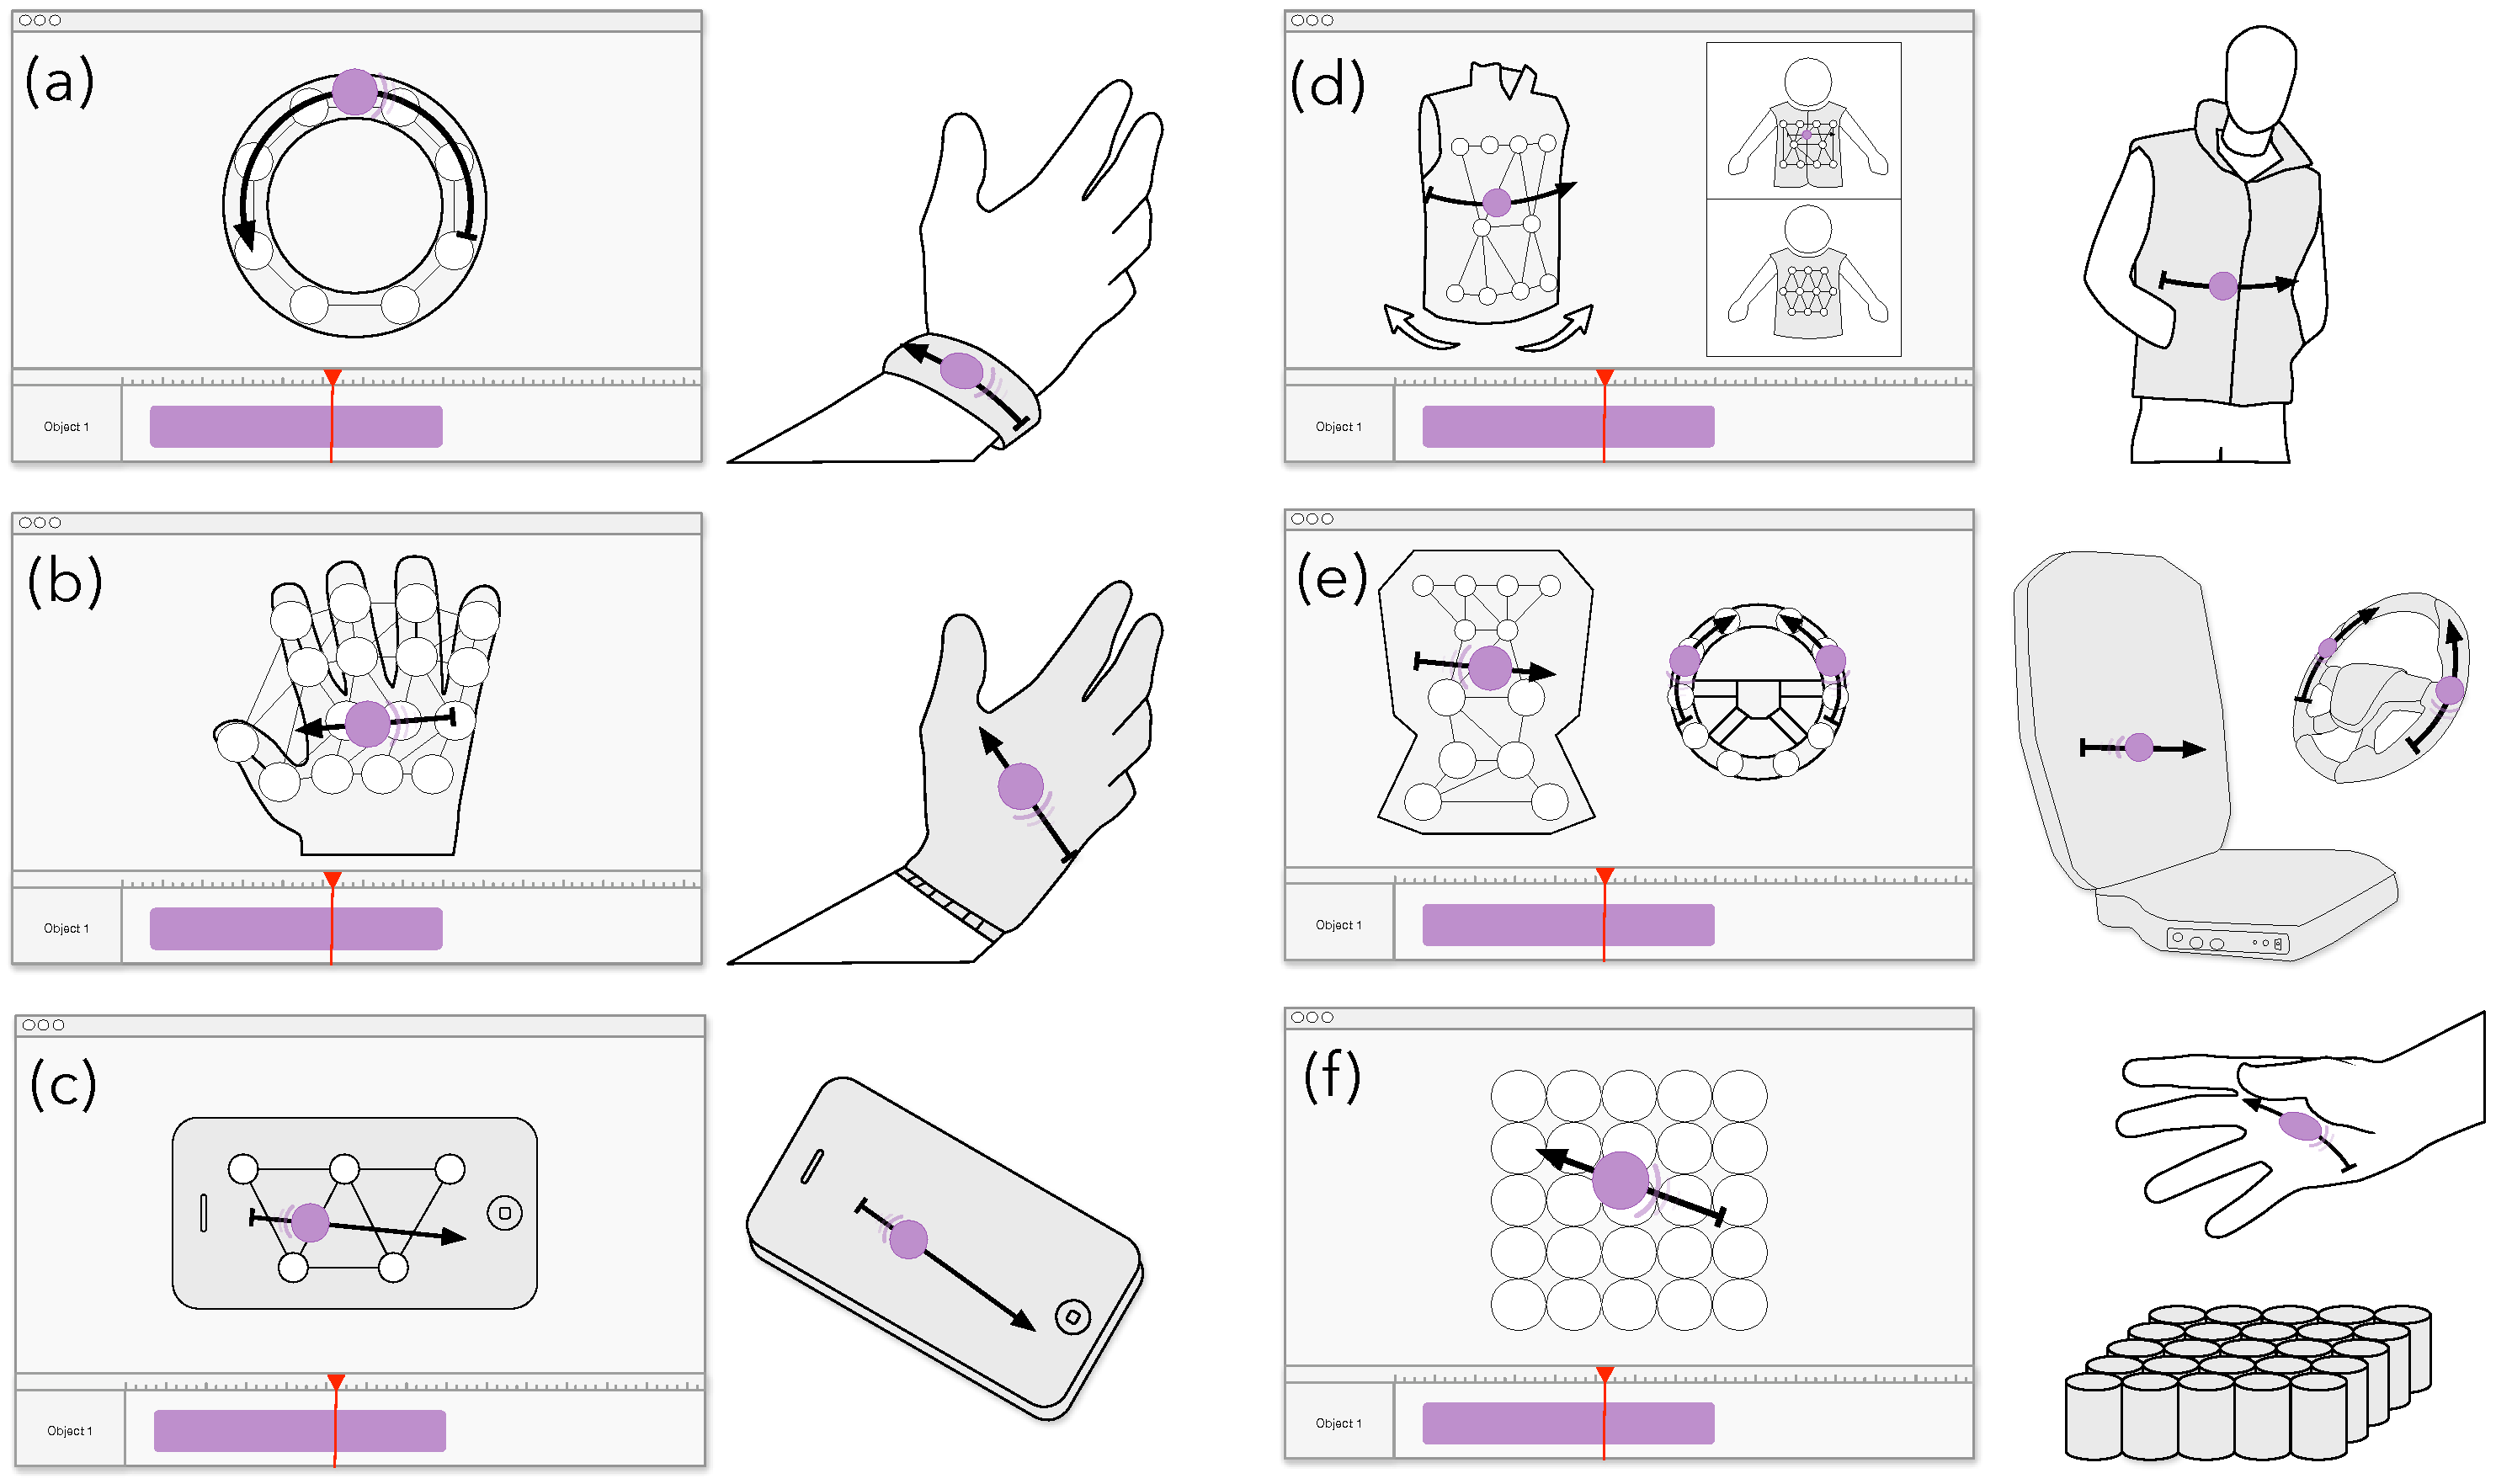
\includegraphics[width=0.8\textwidth]{HA14-Applications-SplitCombined-2015-04-14-1025} 
%   \caption{Tactile animation could define motion with (a) 1D actuator arrays, (b) dense and sparse VT grids, (c) handhelds, d)  3D surfaces, (e) multi-device contexts, and  (f) non-VT devices like mid-air ultrasound.}
%   \label{fig:application:space}
%\end{figure}

%\subsection{Design Evaluation Summary}
%From our design evaluation, we conclude that tactile animation is a promising approach for controlling haptic grid displays.
%Mango facilitated the design of a wide variety of animations (see accompanying video) and positive responses from participants.
%Direct manipulation of tactile animation objects supported embodied design and exploration by animators, who moved the objects to find the right location; this builds on results from the haptic instrument project.
%We also see several recommendations for our next iteration, adding more typical animation features, video as well as audio context, and muting.
%We build on this 

%The tactile animation metaphor also \kmC{orphan? Agree Discussion needs more oomph. Be sure to show balance - point out limitations, what its for vs what its not for, any criticisms raised by users. What stands between it and broader use?}

%%\subsection{Extension to Other Device Classes}
%The animation metaphor is a natural way to express spatial haptics.
%With additional rendering algorithms, some of which are known, we can generalize to other contexts.
%As long a single, spatio-temporal percept can be created, the animation metaphor can be used.
%See \autoref{fig:application:space} for sample applications.



%\vspace{20pt}

%\emph{1D VT Arrays (\autoref{fig:application:space1}a)}:
%1D VT arrays are common in arm sleeves, wrist bands, belts, and similar wearables.
%These devices provide sensations along the path of the array.
%By constraining objects to a linear or circular path, barycentric coordinates collapse into 1D interpolation.
%
%\emph{Dense and Sparse VT Grids  (\autoref{fig:application:space1}b)}:
%2D VT grids are also common, used in chairs, gloves, and the backs of vests.
%%Dense arrays previously had their own actuator-based authoring tools \cite{Kim2009}.
%While we evaluated Mango with a sparse back-mounted array, tactile animation naturally supports denser arrays, either with our rendering algorithm or by using a nearest-neighbour technique to activate a single actuator; in both cases, animation objects can be directly manipulated.
%%In the present work, we evaluated the usability of Mango to author variety of VT sensations on sparse arrays.
%%The actuator layout in both these devices are dif- ferent, and we accomodated them by selecting an appropriate
%%algorithm and layout to render high definition haptic feedback.
%
%
%\emph{Handhelds (\autoref{fig:application:space1}c)}:
%Actuators embedded in handheld objects such as mobile devices, game controllers, or steering wheels shake objects instead of directly stimulating the skin.
%Animators could define source locations for vibrations using handheld-based rendering algorithms (e.g., \cite{Seo2010}).
%%Similarly, a single embedded vibrator in handheld devices can be supported by constraining the tactile object to a single point.
%
%
%\emph{3D Surfaces  (\autoref{fig:application:space2}d)}:
%Mango currently only supports a 2D location for its animation objects.
%However, tactile animation can be extended to support surfaces of 3D surfaces, such as vests or jackets that wrap around the user's body. 
%More work will need to be done to perfect this interaction style, possibly using multiple views or a rotatable 3D model with animation objects constrained to the surface.
%%, drawing more from 3D animation tools like Maya.
%
%\emph{Multi-device contexts  (\autoref{fig:application:space2}e)}:
%Mango's rendering algorithm already supports connections to multiple devices simultaneously.
%The editing interface could combine layouts for different devices, enabling animators to animate the entire user experience (such as a car's seat and steering wheel).
%
%\emph{Non-vibrotactile devices (\autoref{fig:application:space2}f)}:
%While our rendering algorithm is particular to VT arrays, a tactile animation object can represent manipulable percepts with other actuation technologies.
%%Mango is not limited to only VT devices, similar to the one used in the present evaluations.
%Ultrasound-based mid-air displays generate a sensation as a focal point with a position and size \cite{Wilson2014}; this sensation could be manipulated through a tool like Mango.
%% produce a percept of object in mid-air and can be manipu- lated by changing the focal point as a animated object on the Mango interface. Algorithm to generate localize percept can be loaded along with the specifications written in the config- uration file.
%Similarly, passive force-feedback sensations (e.g., Hapseat \cite{Danieau2012a}) or height displays (a grid of pins) could be supported.
%


%\subsection{Interactive Applications}
%While our goal was enabling animators to create rich content, the tactile animation object can be linked to alternative input sources for other interactive experiences.
%
%\emph{User gestures.}
%User gestures and motion can be tracked and mapped to animation objects directly rendered on the haptic hardware.
%For example, a user creates pattens on a touch sensitive tablet that maps touch locations to a grid.
%Users could play games or create personalized haptic messages on the back of a vest.
%Similarly, a dancer's movements could be tracked through accelerometers, drawing animated haptic content on the body of her audience through actuated theater seats during a live performance.
%
%\emph{Camera feed extraction.}
%%Objects from Camera Feed
%Motion of objects from video feeds could be automatically extracted with computer vision and rendered on grid displays, providing dynamic patterns associated with actions during sports, movies, and games.
%Similarly, animation parameters from visual animation tools could be mapped to positions on a VT grid, creating haptic feedback for non-haptic media.
%
%\emph{Data streams.}
%One main application of haptic grid displays is to provide users directional, assistive, and navigational cues during driving cars, walking down the street, or with over-
%saturated sensory tasks.
%Users could associate digital data streams, such as GPS input, to predefined set of directional patterns on the back or palm of the hand.
%
%
%%\subsection{Limitations}
%%While the tactile animation metaphor can be naturally applied in many contexts, there are limitations.
%%Our perceptual study guided our development but does not constitute a full psychophysical investigation.
%%Further work needs to be done to identify the limits, thresholds, and peculiarities of this rendering technique.
%%Second, we only worked with triangular meshes, which might not be appropriate for all grids; quadrilateral interpolation or kernel methods could yield more convincing phantom sensations.
%%Finally, mixing actuator types (such as a chair with both voice coil and rumble motors, \autoref{fig:application:space2}e) could further generalize this approach.
%


\section{Discussion}
The Tactile Animation project expanded our understanding from the Haptic Instrument study in \autoref{ch:hapticinstrument}.
Specifically, it reaffirmed the value of real-time feedback and the need for examples, and showed that a persistent object model reduces cognitive load.
It also suggests again that examples and user experiences are extremely valuable to the design process, providing motivation for example-based haptic design discussed next in \autoref{ch:hapticexamples}.



%%%%%%%%%%
%
%Implications for Design
%
%%%%%%%%%%
%\section{Conclusion}
%
%%This paper presents Mango, a new tactile animation tool to create rich, dynamic and expressive haptic experiences. 
%%The tool utilizes animation metaphor in the design process and renders animated VT patterns on a variety of spatial VT displays.
%%Design requirements gathered in interviews and literature review are implemented on a prototype software that was evaluated with artists and a normal everyday computer user.
%%The post evaluation interviews and feedback suggested that the tool was useful and easily adaptable; and participants highly preferred animation metaphor to design haptic patterns.
%%Overall, tactile animation represents a promising new direction to support haptic media design.
%
%%A key feature of Mango is that it can be used with a wide range of haptic feedback hardware. The hardware specific definitions are provided in the configuration file which facilitates authoring of animations and its rendering on the hardware. Configuration files for new hardware can be constructed and loaded in Mango, to use its authoring capabilities with new hardware.  
%
%%\kmC{Adjust weight: tactile animation then Mango} % Km: up to here, I think it's consistent now. I ran out of steam.
%This paper introduces \emph{tactile animation}, a new approach for creating rich and expressive haptic media on grid displays.
%% The design of Mango is derived from an
%This animation metaphor allows designers and media artists to directly manipulate phantom vibrotactile sensations continuously in both space and time.
%Our rendering pipeline, which uses a perceptually-guided phantom sensation algorithm, enables critical real-time feedback for designing.
%%an approach that is more direct and potentially creative than coordinating individual actuators, and which scales better to large actuator maps, where perceived motion is nearly intractable using track-based approaches.
%%Unlike previous tools that either required rigorous programming background or was applicable to a specific hardware configuration, an animation approach also % our tool
%%provides a familiar interface to a large animation workforce, therefore eliminating training time and cost necessary for haptic content production in the mainstream media.  
%We incorporated these ideas into a prototype, Mango, with a design grounded in animator requirements and haptic design guidelines.
%Professional animators used our tool to create a variety of designs, giving positive feedback and excitement for future versions.
%This approach has the potential to % KM: concerned that this functionality can be added to any tool with properly designed configuration files, and isn't tied particularly to the other innovations reported here. If so, need to be much more careful about how it's phrased since this capability isn't even really demonstrated here - you only use one display apparatus.
%% Moreover, Mango 
%accommodate a large variety of haptic hardware, ranging from a single shaking element mounted on the seat to an array of actuators stimulating multiple points on the skin, and can export content into formats applicable in the production pipeline.
%Tactile animation empowers animators with a new set of artistic tools for rich, multimodal feedback. 
%
%\bibliographystyle{acmsiggraph}
%\bibliography{HA14-CHI2015,HA14-CHI2015-SIGGRAPH-add,verillo2}
\endinput



\chapter{Combine: Design Galleries}
\label{ch:hapticexamples}

\begin{figure}[htbp]
\begin{center}
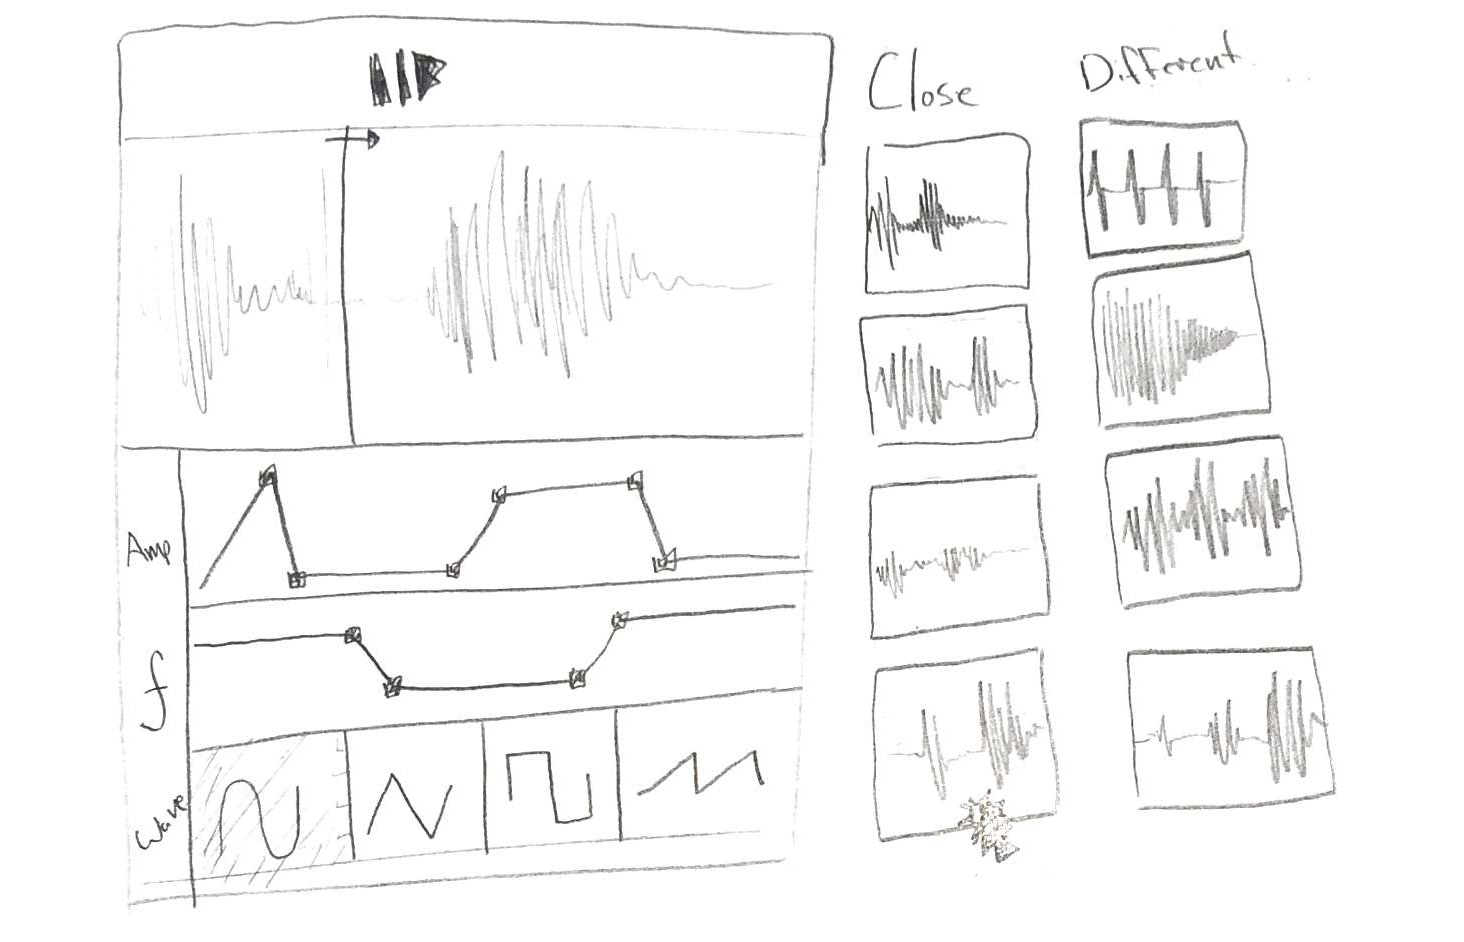
\includegraphics[width=4in, height=2.17in]{VTDesignGallerySketch}

\caption{Concept sketch for a vibrotactile design gallery.}
\label{hapticexamples:designgallerysketch}
\end{center}
\end{figure}

In both the Haptic Instrument and Tactile Animation case studies, participants drew from their experience or external examples and requested features for repetition.
This is unsurprising; creative tasks, like design, are often defined as the recombination of existing ideas, with a twist of novelty or spark of innovation by the individual creator \cite{Warr2005}.
Examples are critical to provide inspiration, guidance, and inform design \cite{Herring2009,Buxton2007}; for example,
%In other fields of design, designers clip, store, and display examples for inspiration \cite{Buxton2007}.
industrial designers collect various knobs and materials, and web designers bookmark sites \cite{Herring2009}.
Managing these examples effectively is already a significant task even in these more visual fields, but there is no explicit support for vibrotactile (VT) design.
I will investigate interaction techniques to directly use examples in haptic design through a design gallery tool for VT icons (\autoref{hapticexamples:designgallerysketch}).



Design galleries are used in graphics and web design to facilitate the use of examples \cite{Lee2010a,Marks1997}.
While there are several challenges involved with examples in design, including capture, search, management, use, and sharing, I limit this project's scope to the \emph{combining} existing examples to create new VT icons.
This project takes place in two phases: Phase I, where we develop a set of tools to manipulate VT icons through interpolation and combination, and Phase II, creating a design gallery and investigating how users work with it (or would like to, if they are unable to do so).
For this study, we use a single Haptuator bound to a mobile device to simulate mobile VT icons (\autoref{fig:macarondevice}).


%\begin{figure}[htbp]
%\begin{center}
%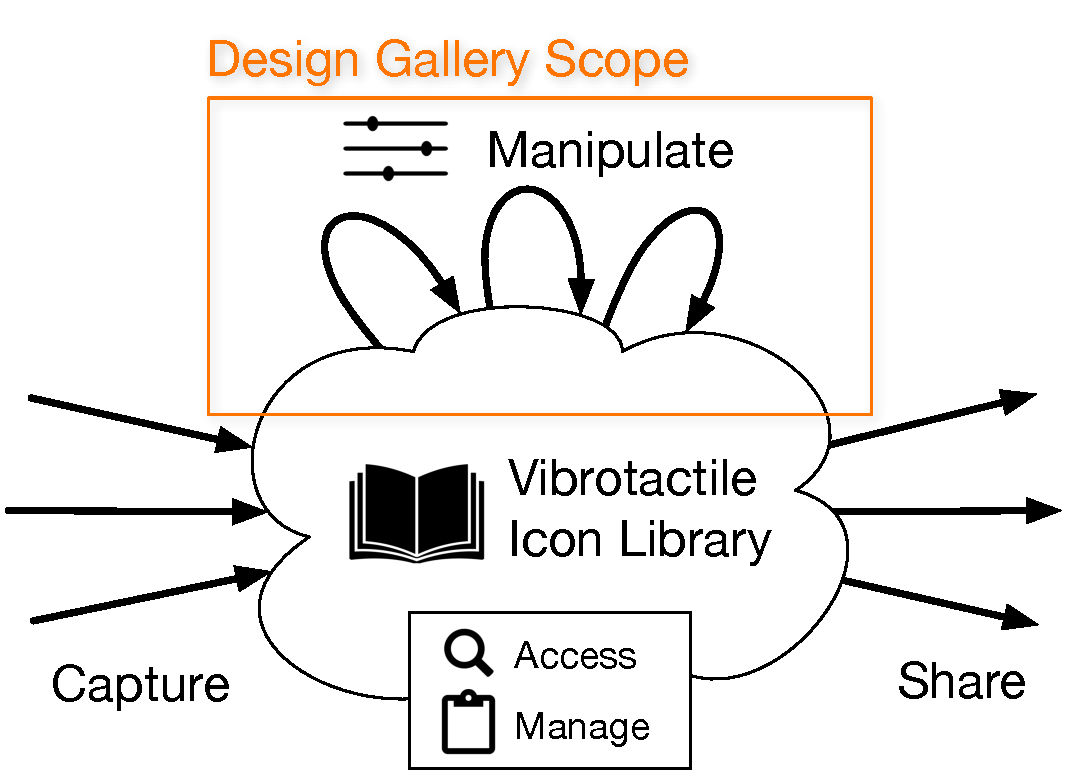
\includegraphics[width=0.4\textwidth]{ExamplesEcosystem}
%
%\caption{Example ecosystem and design gallery scope.}
%\label{hapticexamples:overview}
%\end{center}
%\end{figure}



\begin{figure}[htbp]
 \centering
   \begin{subfigure}[t]{0.35\textwidth}
	  \centering
	   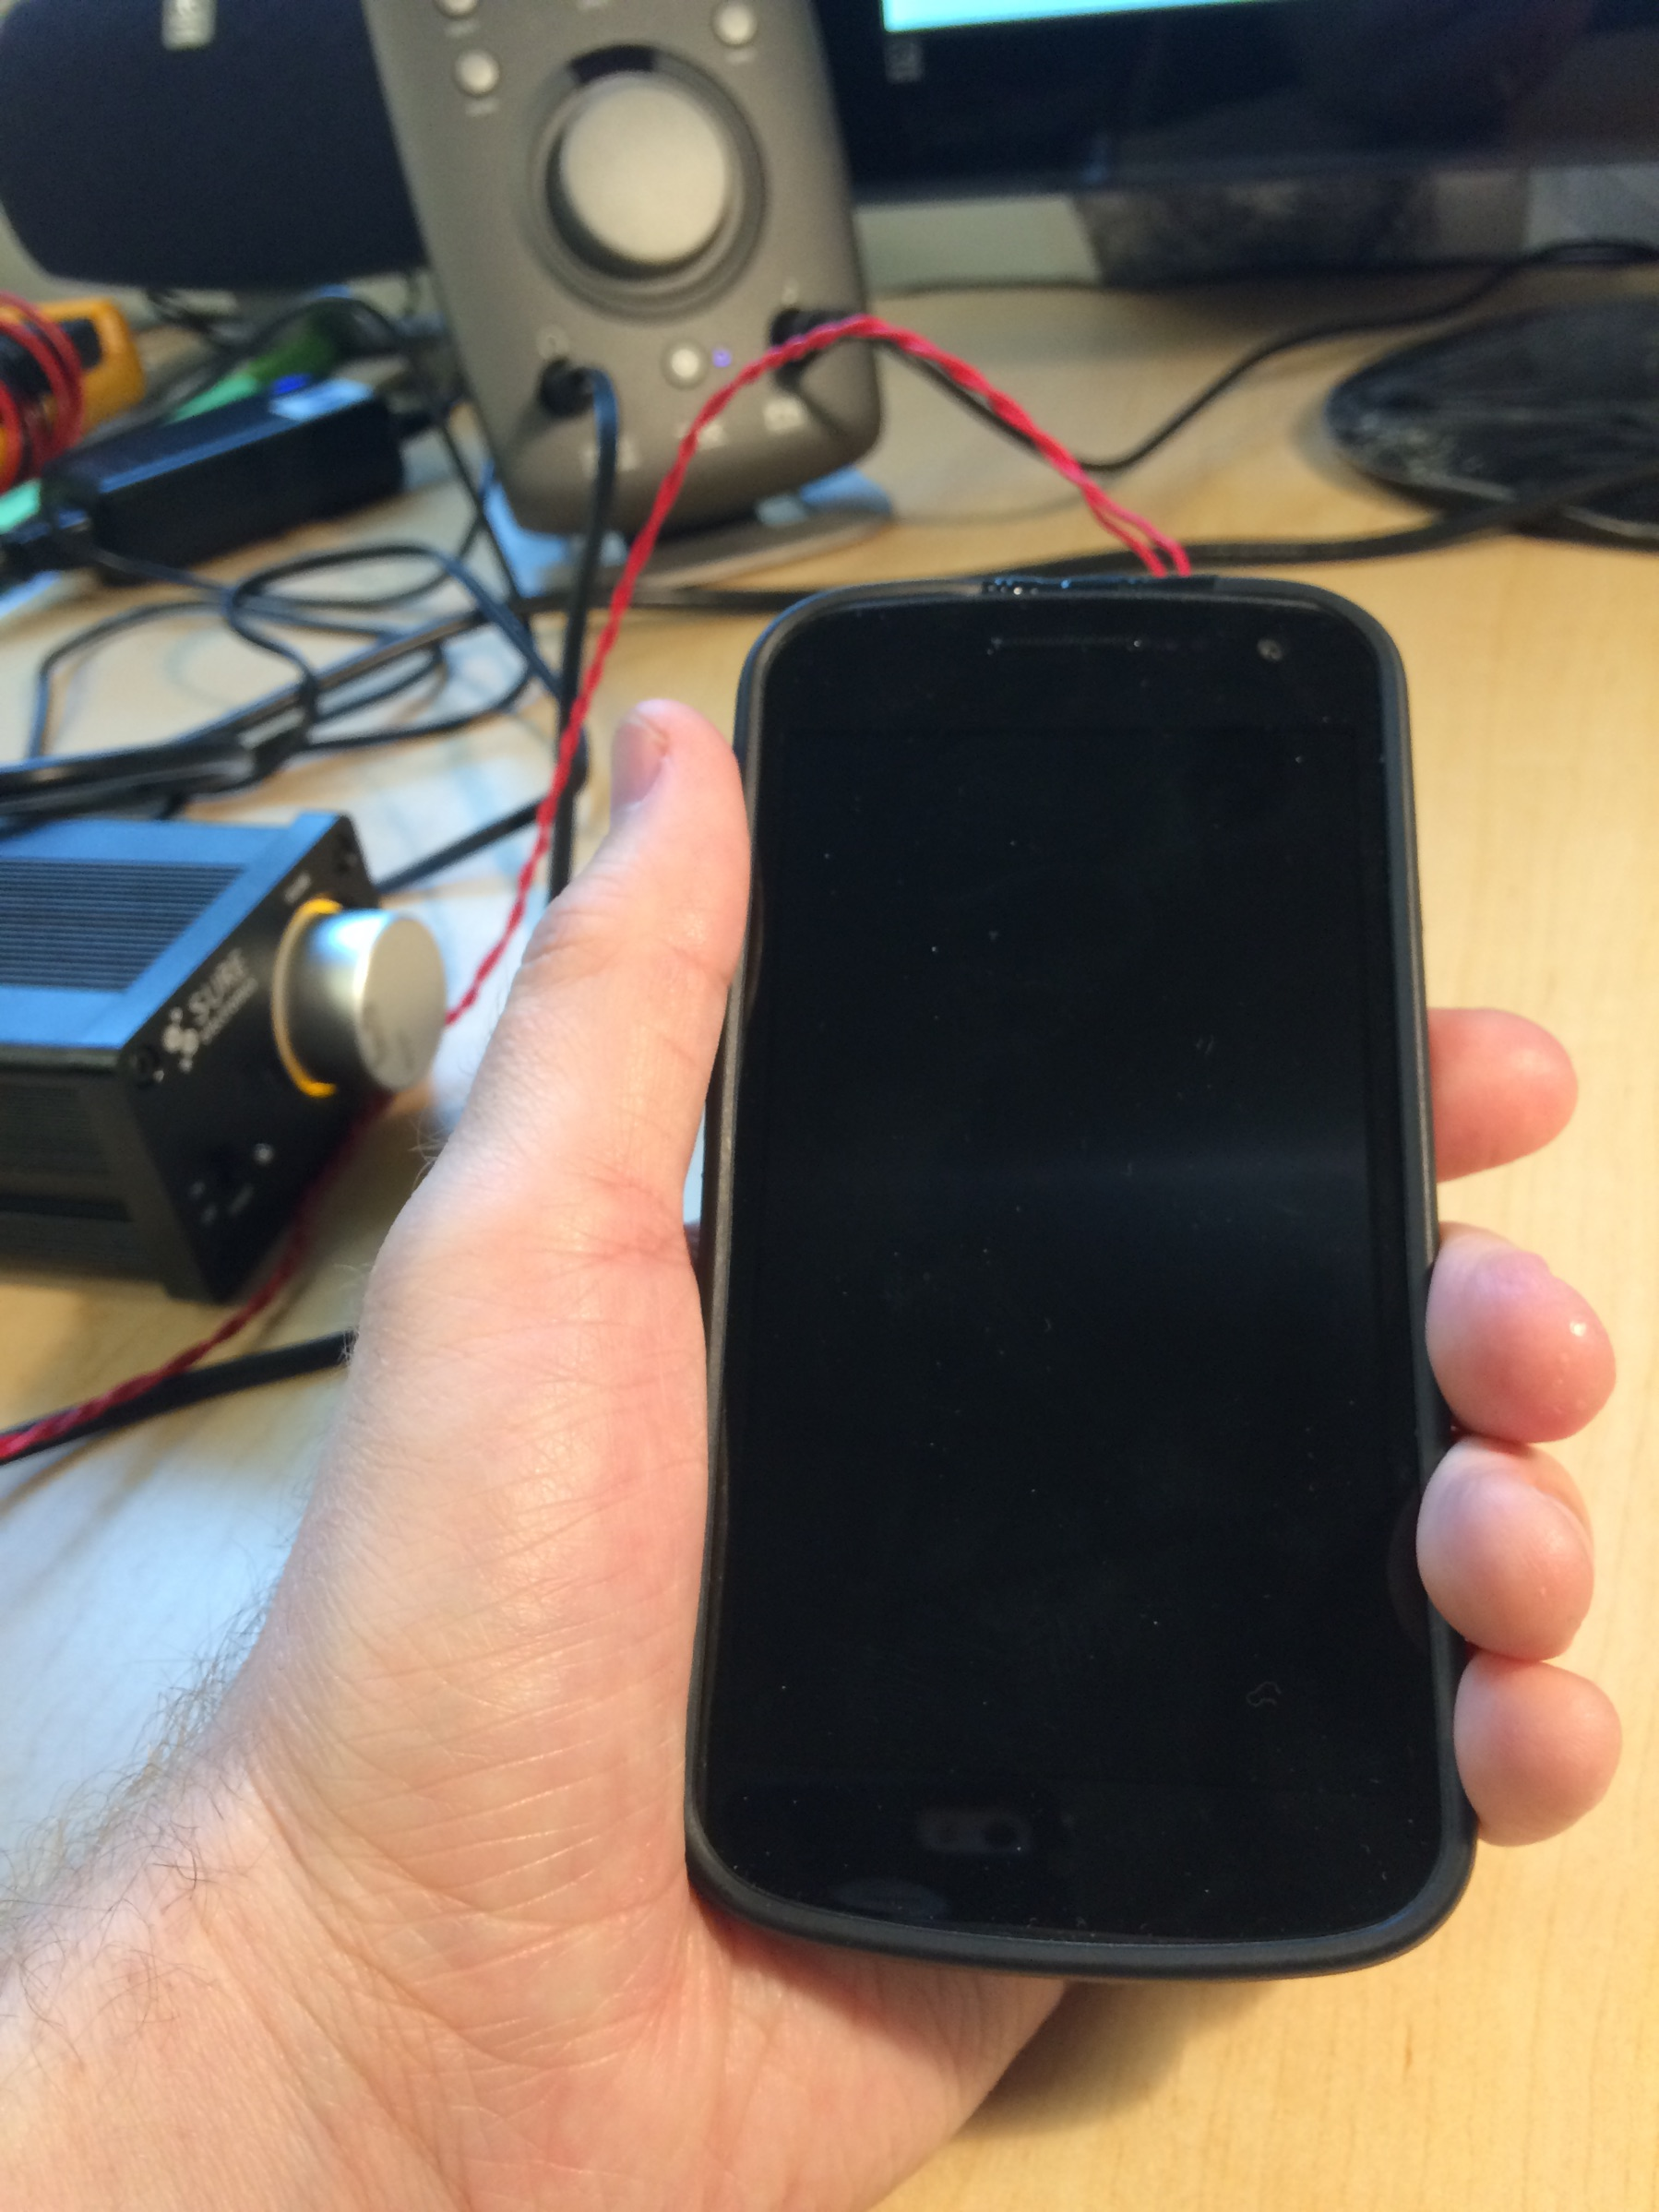
\includegraphics[width=\textwidth, clip=true, trim=0 200 0 0]{macaron-device1} 
	   \label{fig:macarondevice:front}
    \end{subfigure}
    \qquad
     \begin{subfigure}[t]{0.35\textwidth}
	  \centering
	   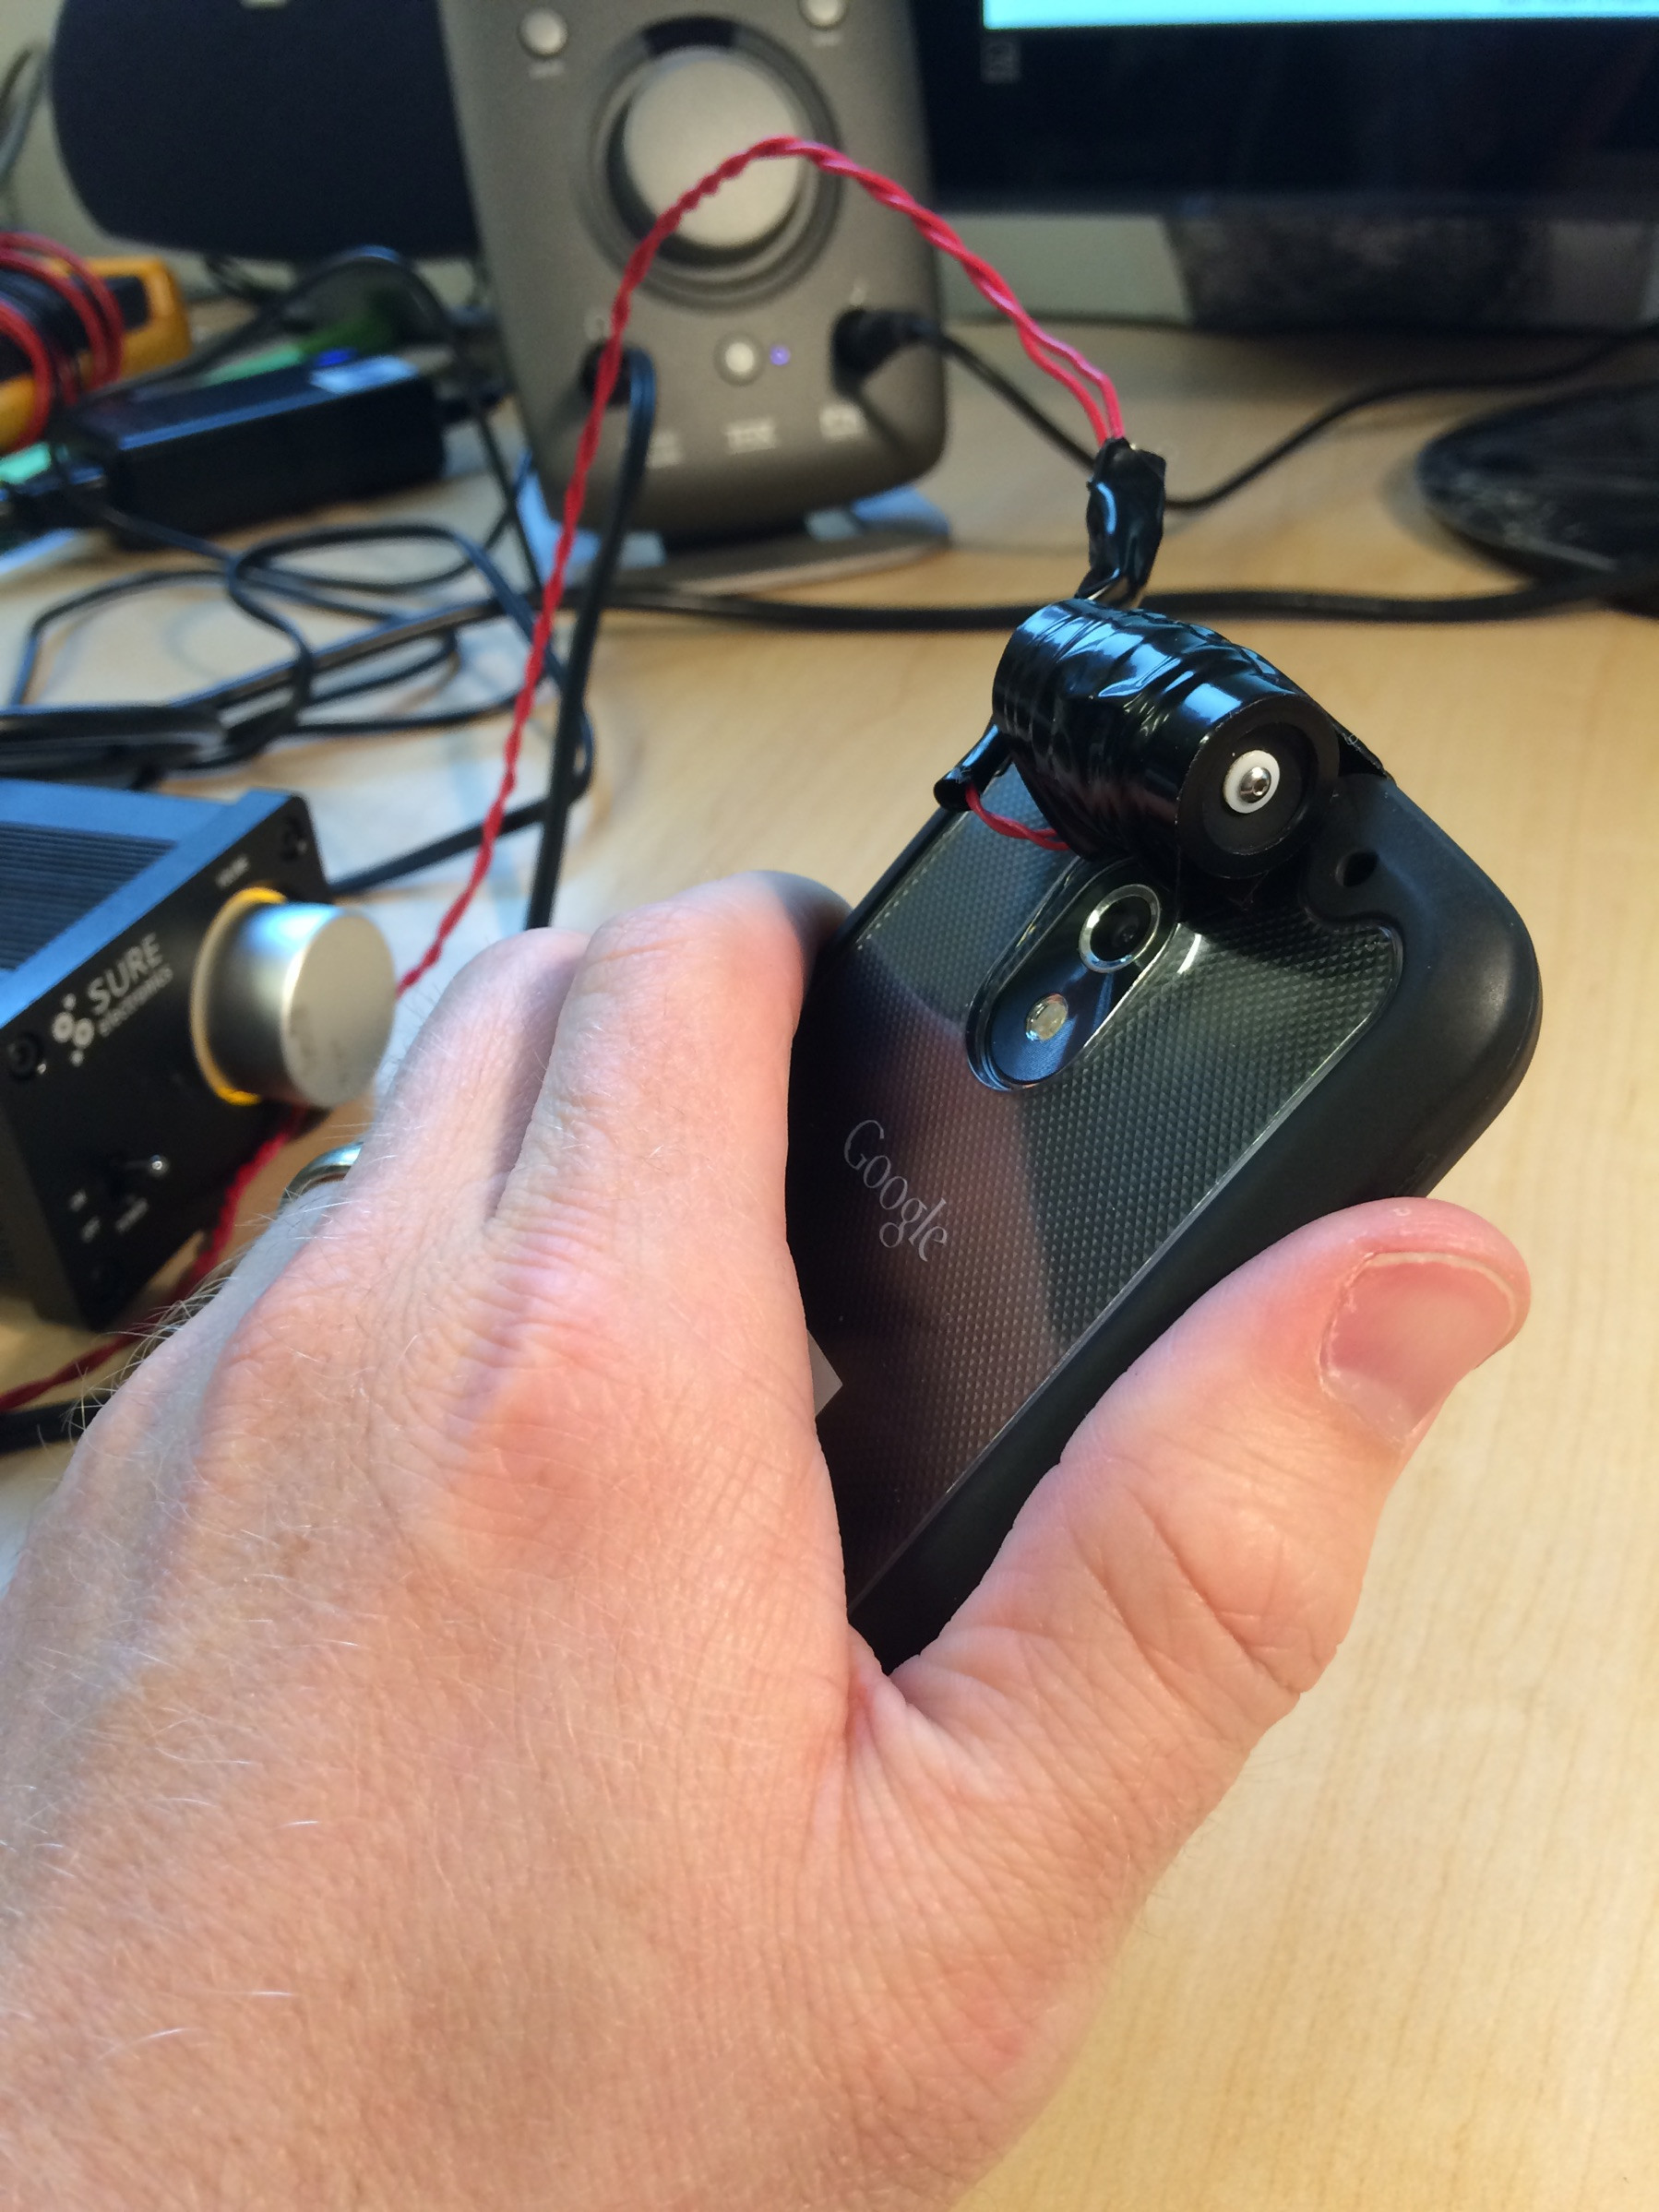
\includegraphics[width=\textwidth, clip=true, trim=0 200 0 0]{macaron-device2} 
	   \label{fig:macarondevice:back}
    \end{subfigure}

    \caption{Apparatus. A Haptuator is mounted onto a Galaxy Nexus smartphone to simulate mobile VT icon development, similar to \cite{InwookHwang2013}.}
    \label{fig:macarondevice}
\end{figure}


\section{Phase I -- Algorithms and Interaction Techniques}
In Phase I, I will develop and evaluate algorithms for manipulating examples by adjusting low-level parameters (frequency, amplitude, duration, and waveform), interpolating between examples, and combining aspects of different examples (for example, combining the frequency profile of one example with the amplitude profile of another). These algorithms will be evaluated using a perceptual study to examine two criteria: a smooth, linear interpolation method between VT icons, and to produce a varied corpus of VT icons.

\subsection{VT Icon Editing}
The design parameters of VT icons are already well understood to be frequency, amplitude, waveform, rhythm, and location.
In this study, we focus on a single actuator display.
Direct editing is supported with a track-based editor, similar to previous work \cite{Swindells2006}, using keyframes like those in the tactile animation prototype, Mango, with one track each for frequency, amplitude, and waveform.
These tracks constitute envelopes of each parameter over the duration of the VT icon.
Rhythm emerges as the amplitude envelope.
In order to use waveform as a time-varying parameter, we crossfade between phase-synchronized waveforms, as used with haptic knobs in \cite{MacLean2009a}.
As this would be the first instance of continuous, time-varying waveform as a VT design parameter, we validate using piloting.
A more thorough study would be valuable to the VT literature, but is secondary to our research questions about the design process.

\subsection{VT Icon Replacement}
In addition to directly editing parameters, we want to enable using examples directly in the design process.
By using a track-based approach to VT icons,  we get another interaction technique: full or partial replacement.
In a design gallery, users can select an icon as a starting point, which we call \emph{full replacement}.
However, tracks can also be replaced, as long as some normalization technique is applied to accommodate different durations.
This \emph{partial replacement} is a weak form of example-based design, where users can combine examples in a limited way to create a new VT icon.
A richer tool would be to more fluidly morph between icons.


\begin{figure}[htbp]
\begin{center}
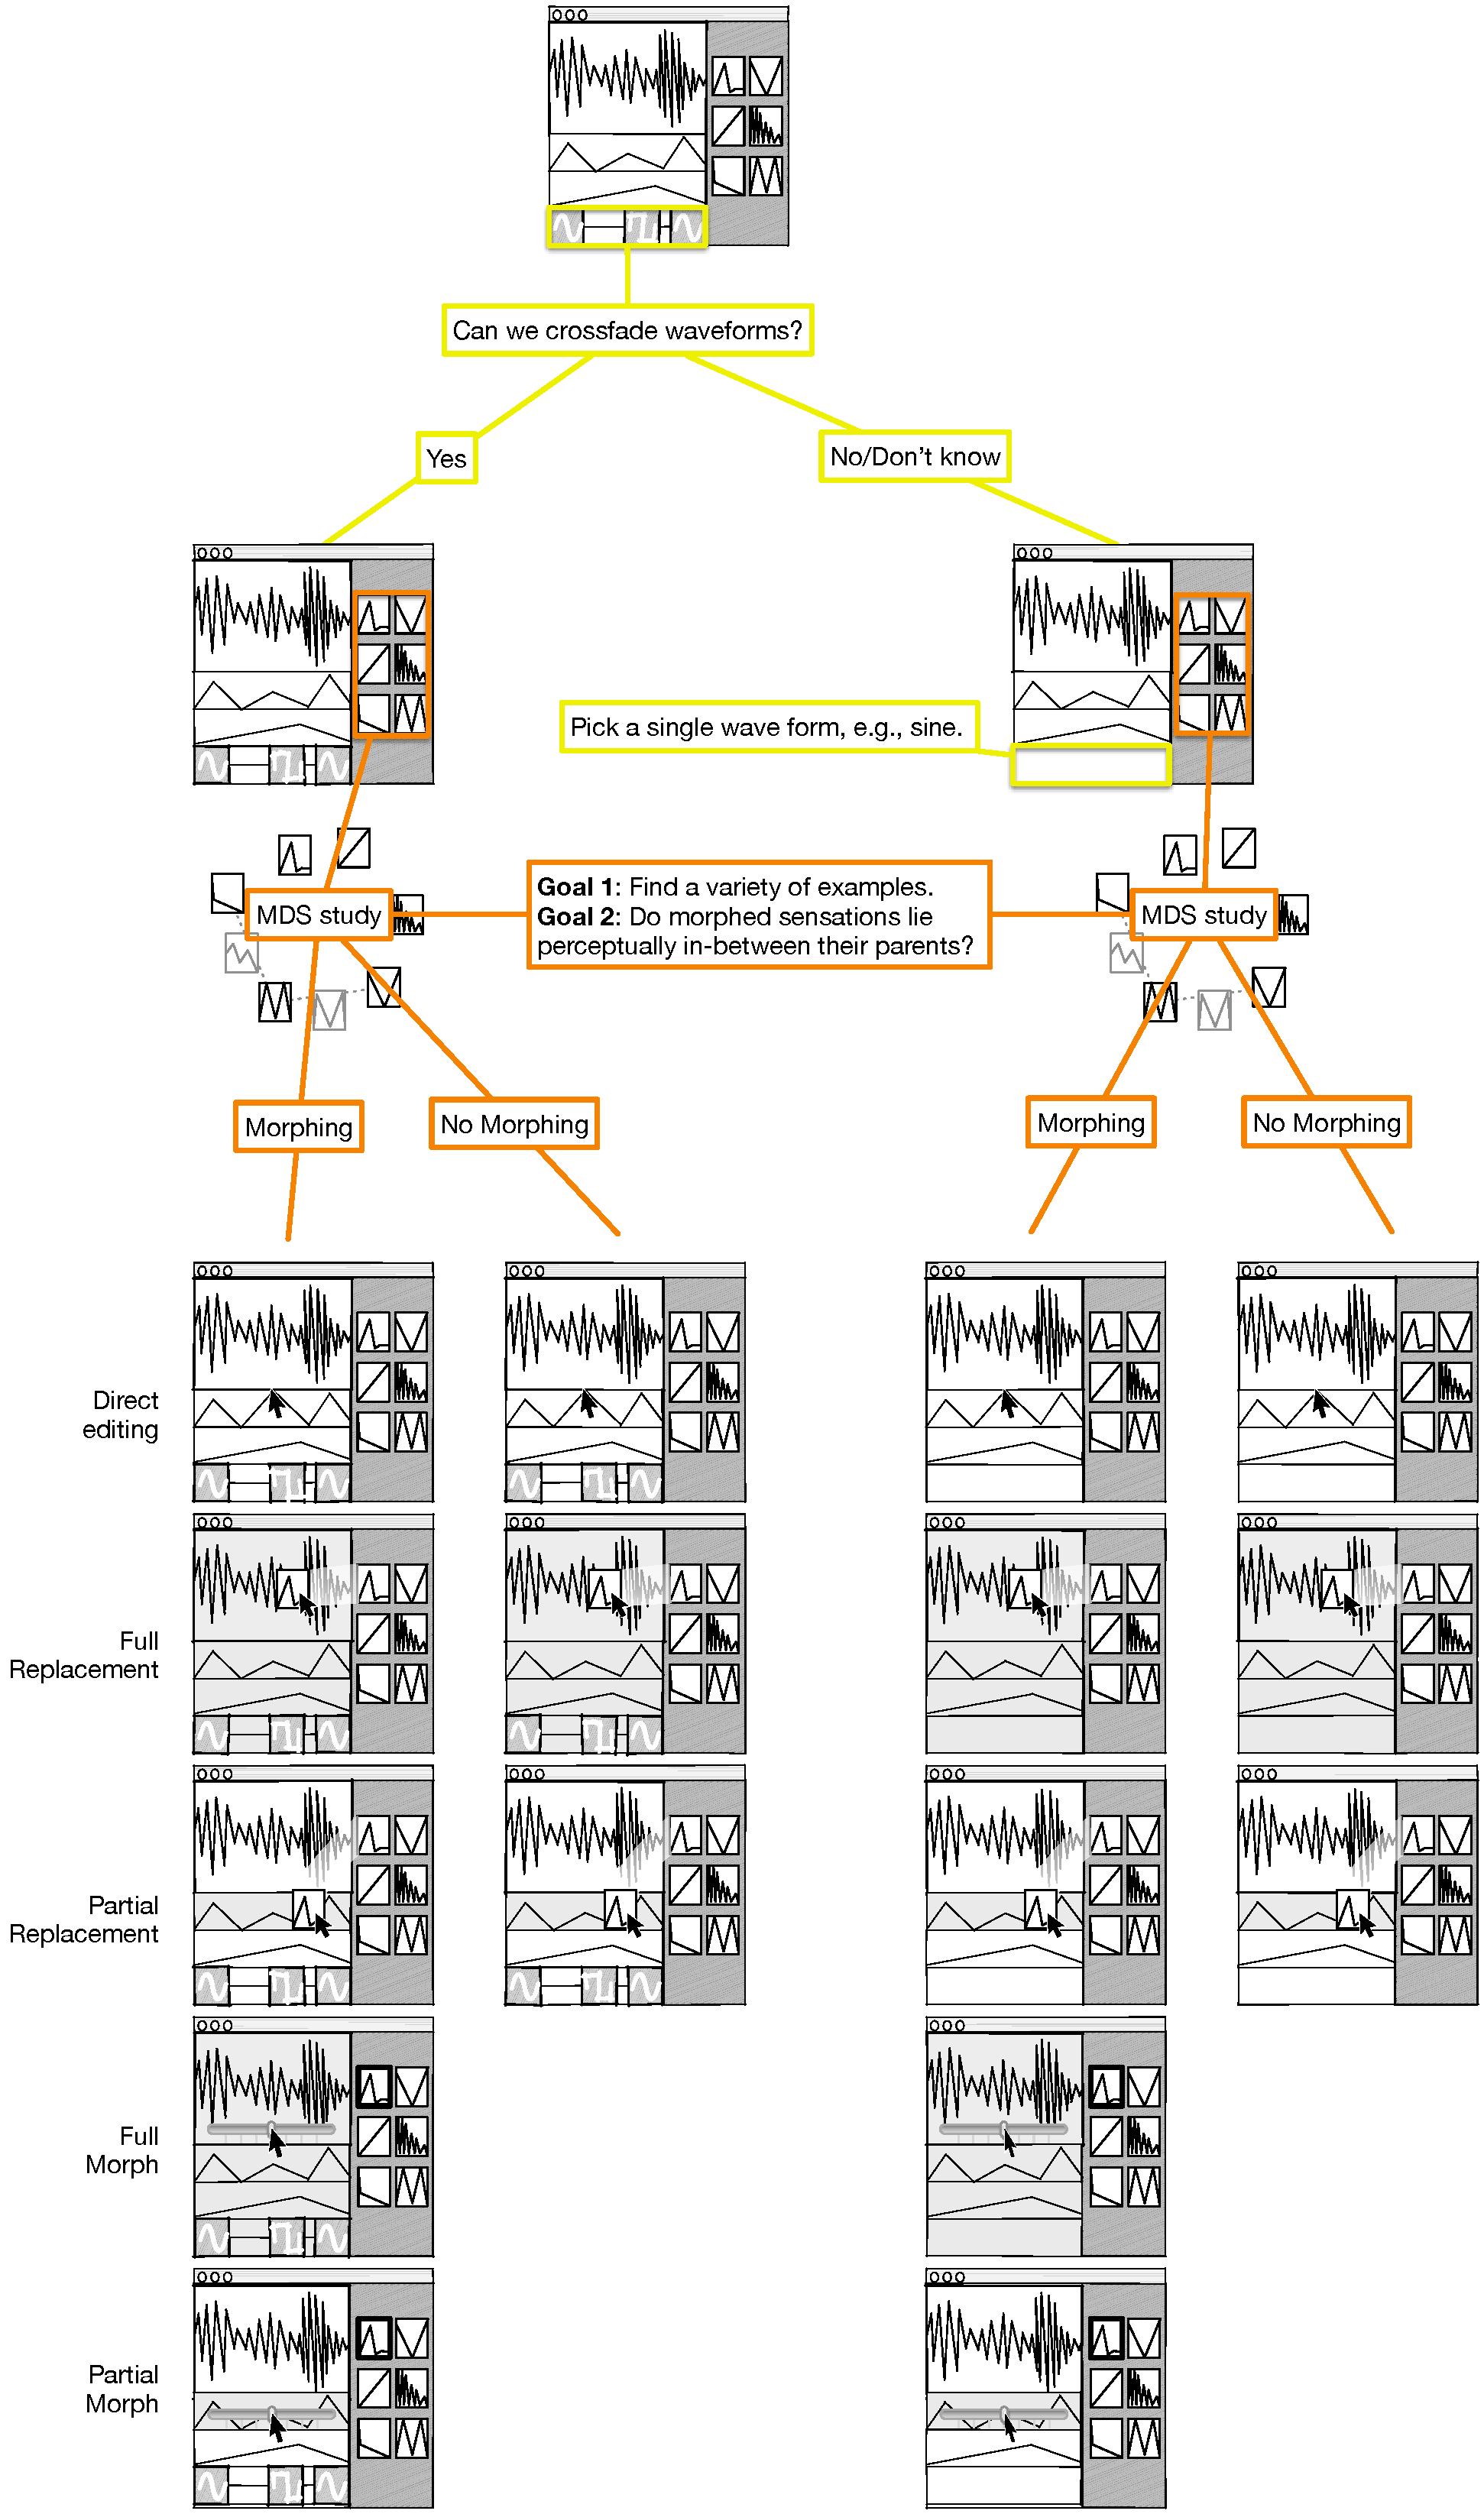
\includegraphics[width=0.7\textwidth, height=0.8\textheight]{HapticExamples-MorphingOrNot}

\caption{Phase I overview, with possible outcomes. We 1) pilot crossfading between waveforms, and 2) conduct an MDS study to find perceptually varied icons and evaluate morphing. The end result is a set of interaction techniques suitable for Phase II.}
\label{fig:macaron:phaseI:overview}
\end{center}
\end{figure}

\subsection{Morphing}
I propose to develop a \emph{morphing} algorithm for VT icons, based on dynamic time warping (DTW) of keyframes in each of the parameter tracks.
The goal is to have a linear, perceptually-smooth transition between VT icons that lets users mix examples, much like a painter might mix colours from a palette.
Similar to VT icon replacement, morphing could be between entire VT Icons (\emph{full morphing}), or between tracks (\emph{partial morphing}).

\subsection{Multidimensional Scaling Study}
To evaluate the morphing algorithm, and to develop a suitable set of VT icons for Phase II, I plan to conduct a multidimensional scaling (MDS) study.
MDS is a psychophysical technique that uses similarity scores between stimuli to build a visualization along underlying perceptual dimensions.
We can use this study to find two results:
\begin{enumerate}
\item From an initial set of 20-30 VT icons, we can identify clusters of similar icons, and select a diverse set of examples for Phase II.
\item By including a VT icons produced by the morphing algorithm, we can see whether they lie on a smooth perceptual path between their parent icons. If so, the morphing algorithm does indeed provide a perceptually smooth transition between parents. 
\end{enumerate}

The possible outcomes for Phase I are visualized in \autoref{fig:macaron:phaseI:overview}.



\section{Phase II -- Design Gallery Development and Evaluation}
In Phase II, I will develop a design tool that implements these algorithms, and use it to study how users involve examples in their designs.
An HTML/JavaScript prototype is under development (\autoref{fig:macaron:phaseII:prototype}), which generates sound that is streamed to the Haptuator through the audio jack.
Our questions and planned studies are visualized in \autoref{fig:macaron:phaseII:overview}.

\begin{figure}[h]
\centering
 \begin{subfigure}[t]{0.4\textwidth}
	\begin{center}
	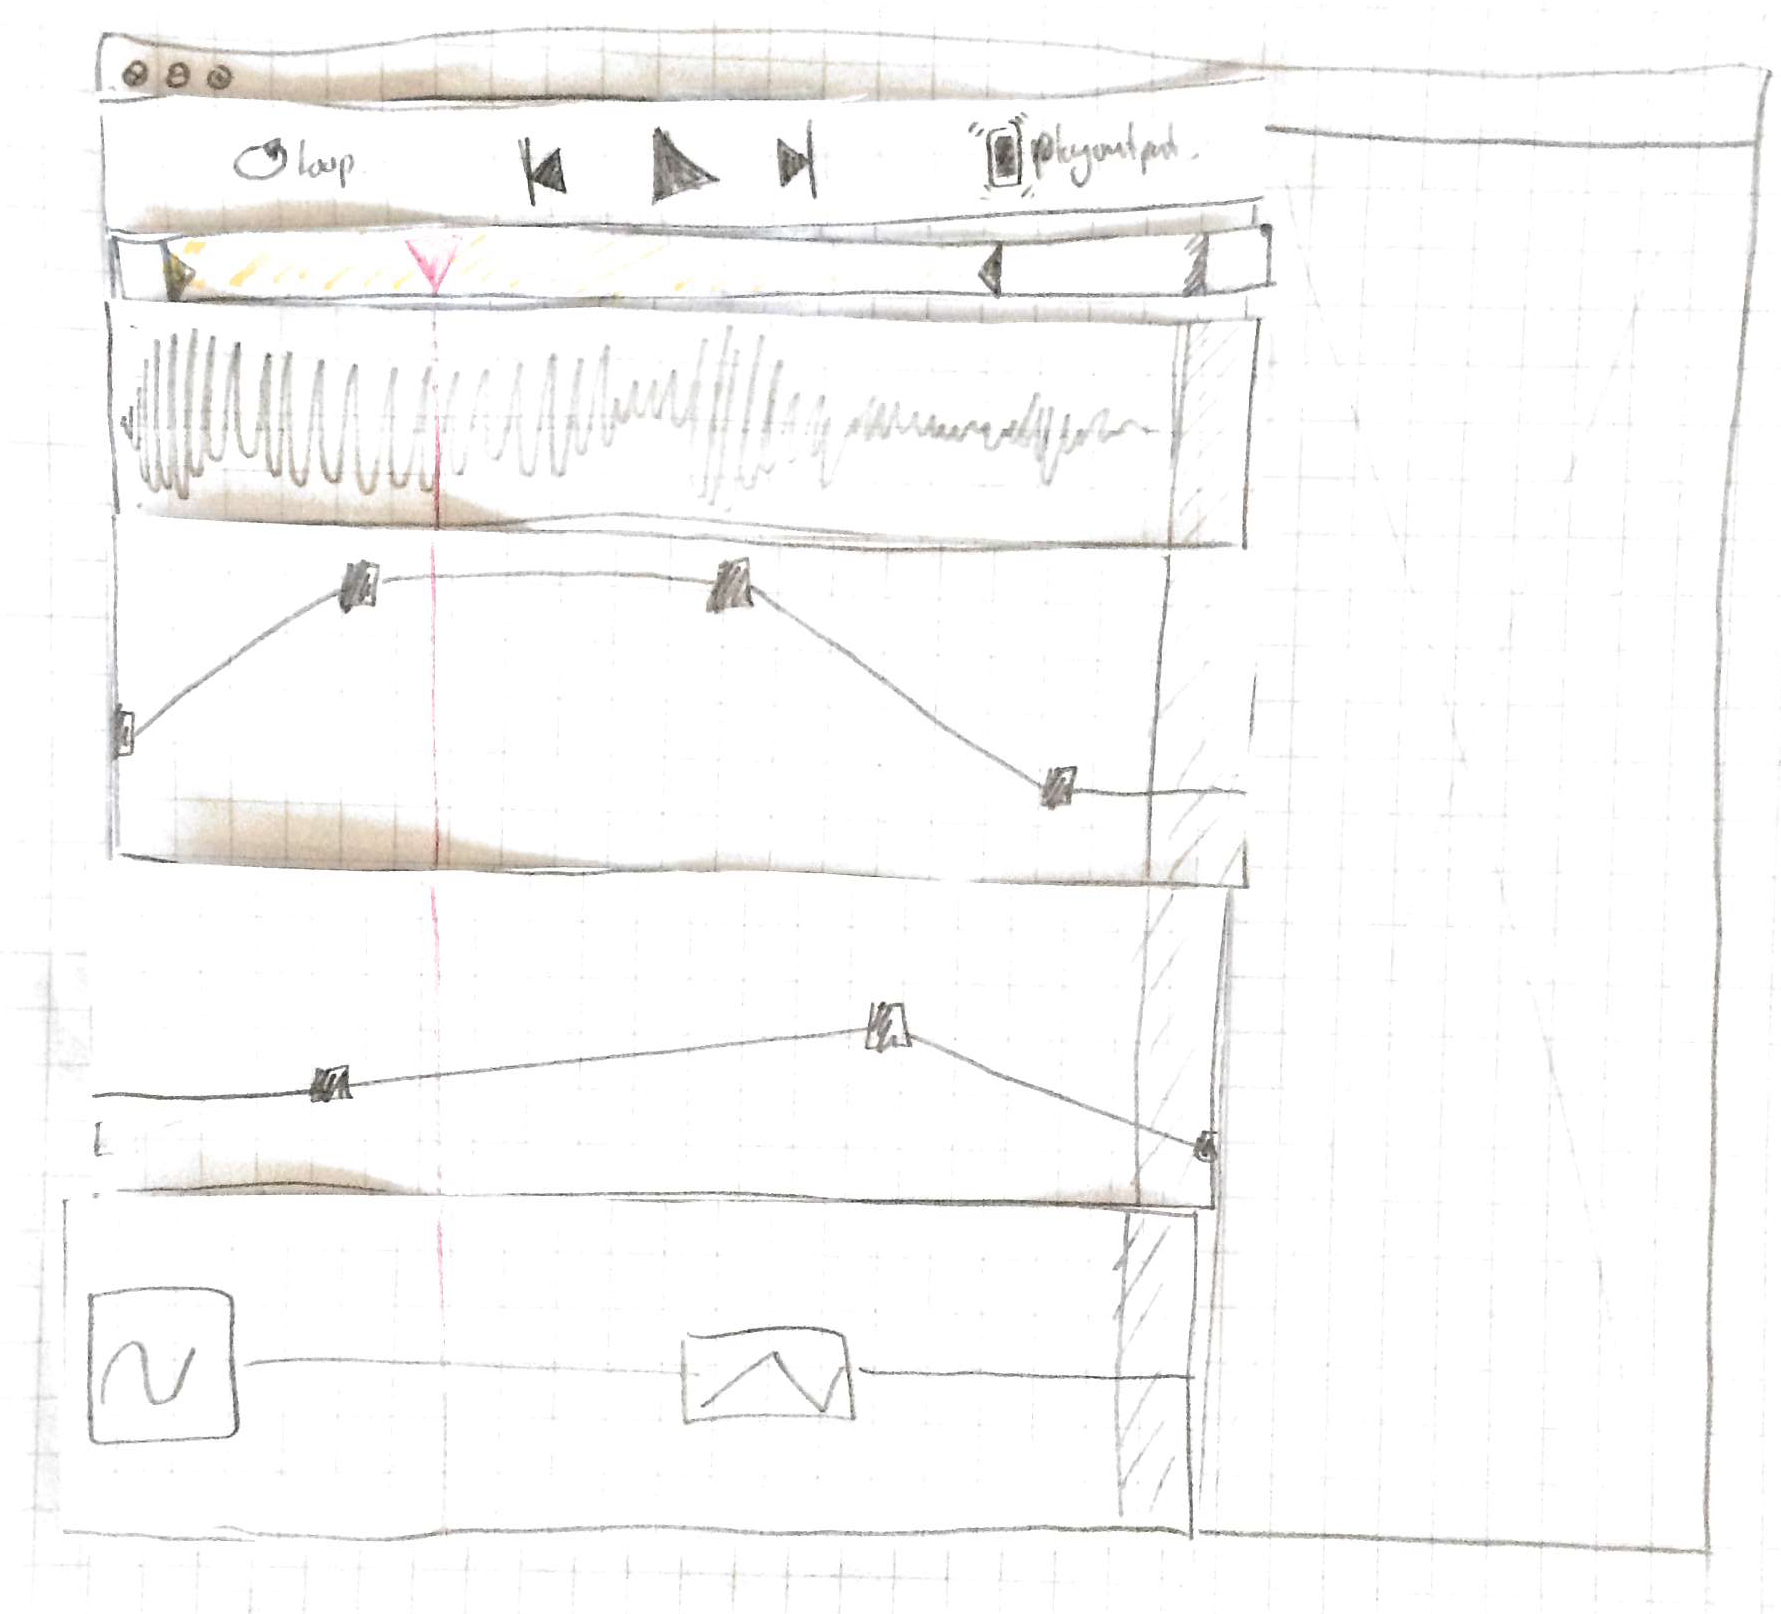
\includegraphics[width=\textwidth]{InitialMacaronEditorPaperPrototypeCropped}
	\caption{Paper prototype.}
	\label{fig:macaron:phaseII:prototype:paper}
	\end{center}
    \end{subfigure}
 ~
 \begin{subfigure}[t]{0.4\textwidth}
	\begin{center}
	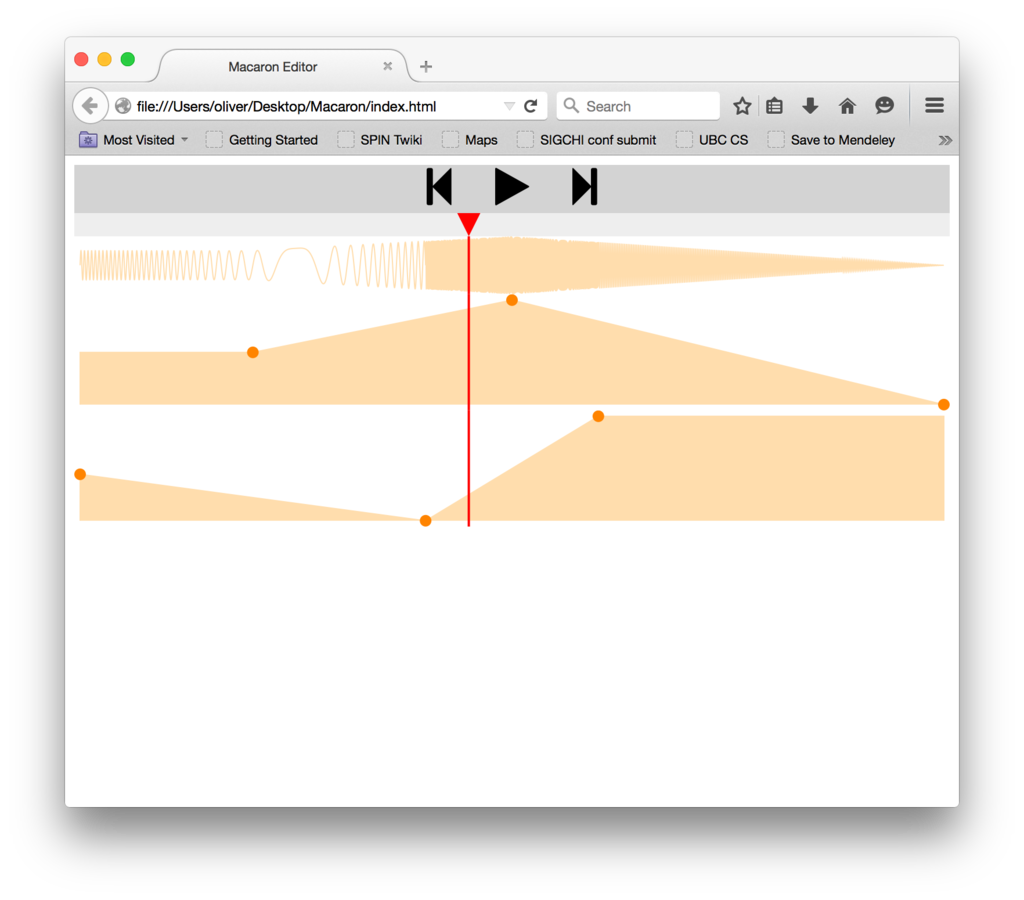
\includegraphics[width=\textwidth]{MacaronEditorScreenshot-2015-05-12}
	\caption{HTML/JavaScript prototype.}
	\label{fig:macaron:phaseII:prototype:html}
	\end{center}
    \end{subfigure}
	
	\caption{Initial prototypes for Macaron Editor.}
	\label{fig:macaron:phaseII:prototype}

\end{figure}




\section{Deliverables and Risk}

This project is intended to be completed in fall 2015, with a planned paper submission to CHI'16 or HAPTICS'16 (deadline in September), DIS'16 (deadline expected in December), or a similar venue.
I mitigate risk in following ways.
%However, given the number of side-projects scheduled in summer 2015, it's possible that this timeframe will be extended.
Phase I studies are designed to result in actionable results with or without waveform crossfading and morphing (\autoref{fig:macaron:phaseI:overview}).
If vibrotactile icons are not found to be diverse, I can select icons via piloting or from the HapTurk side project, which currently has a diverse set of icons selected.
Phase II studies are also designed to robustly provide results; we are primarily describing what users are doing.
If our system encounters technical problems, we can adjust the scope to mitigate risk, focusing more or less on Phase I or Phase II.
For example, if Phase II runs into unforeseen problems, we can submit a focused piece on Phase I (algorithms and interaction techniques) with more thorough investigation of morphing or waveform crossfading.
Alternatively, if Phase I encounters much difficulty, we can extend Phase II and look more at user interactions and less at algorithms.
Finally, if both Phases are compromised due to implementation problems, we can study these research questions by extending a previous tool: mHIVE, Mango, FeelCraft, and Feel Messenger could all be extended to investigate similar research questions.


\begin{figure}[htbp]
\begin{center}
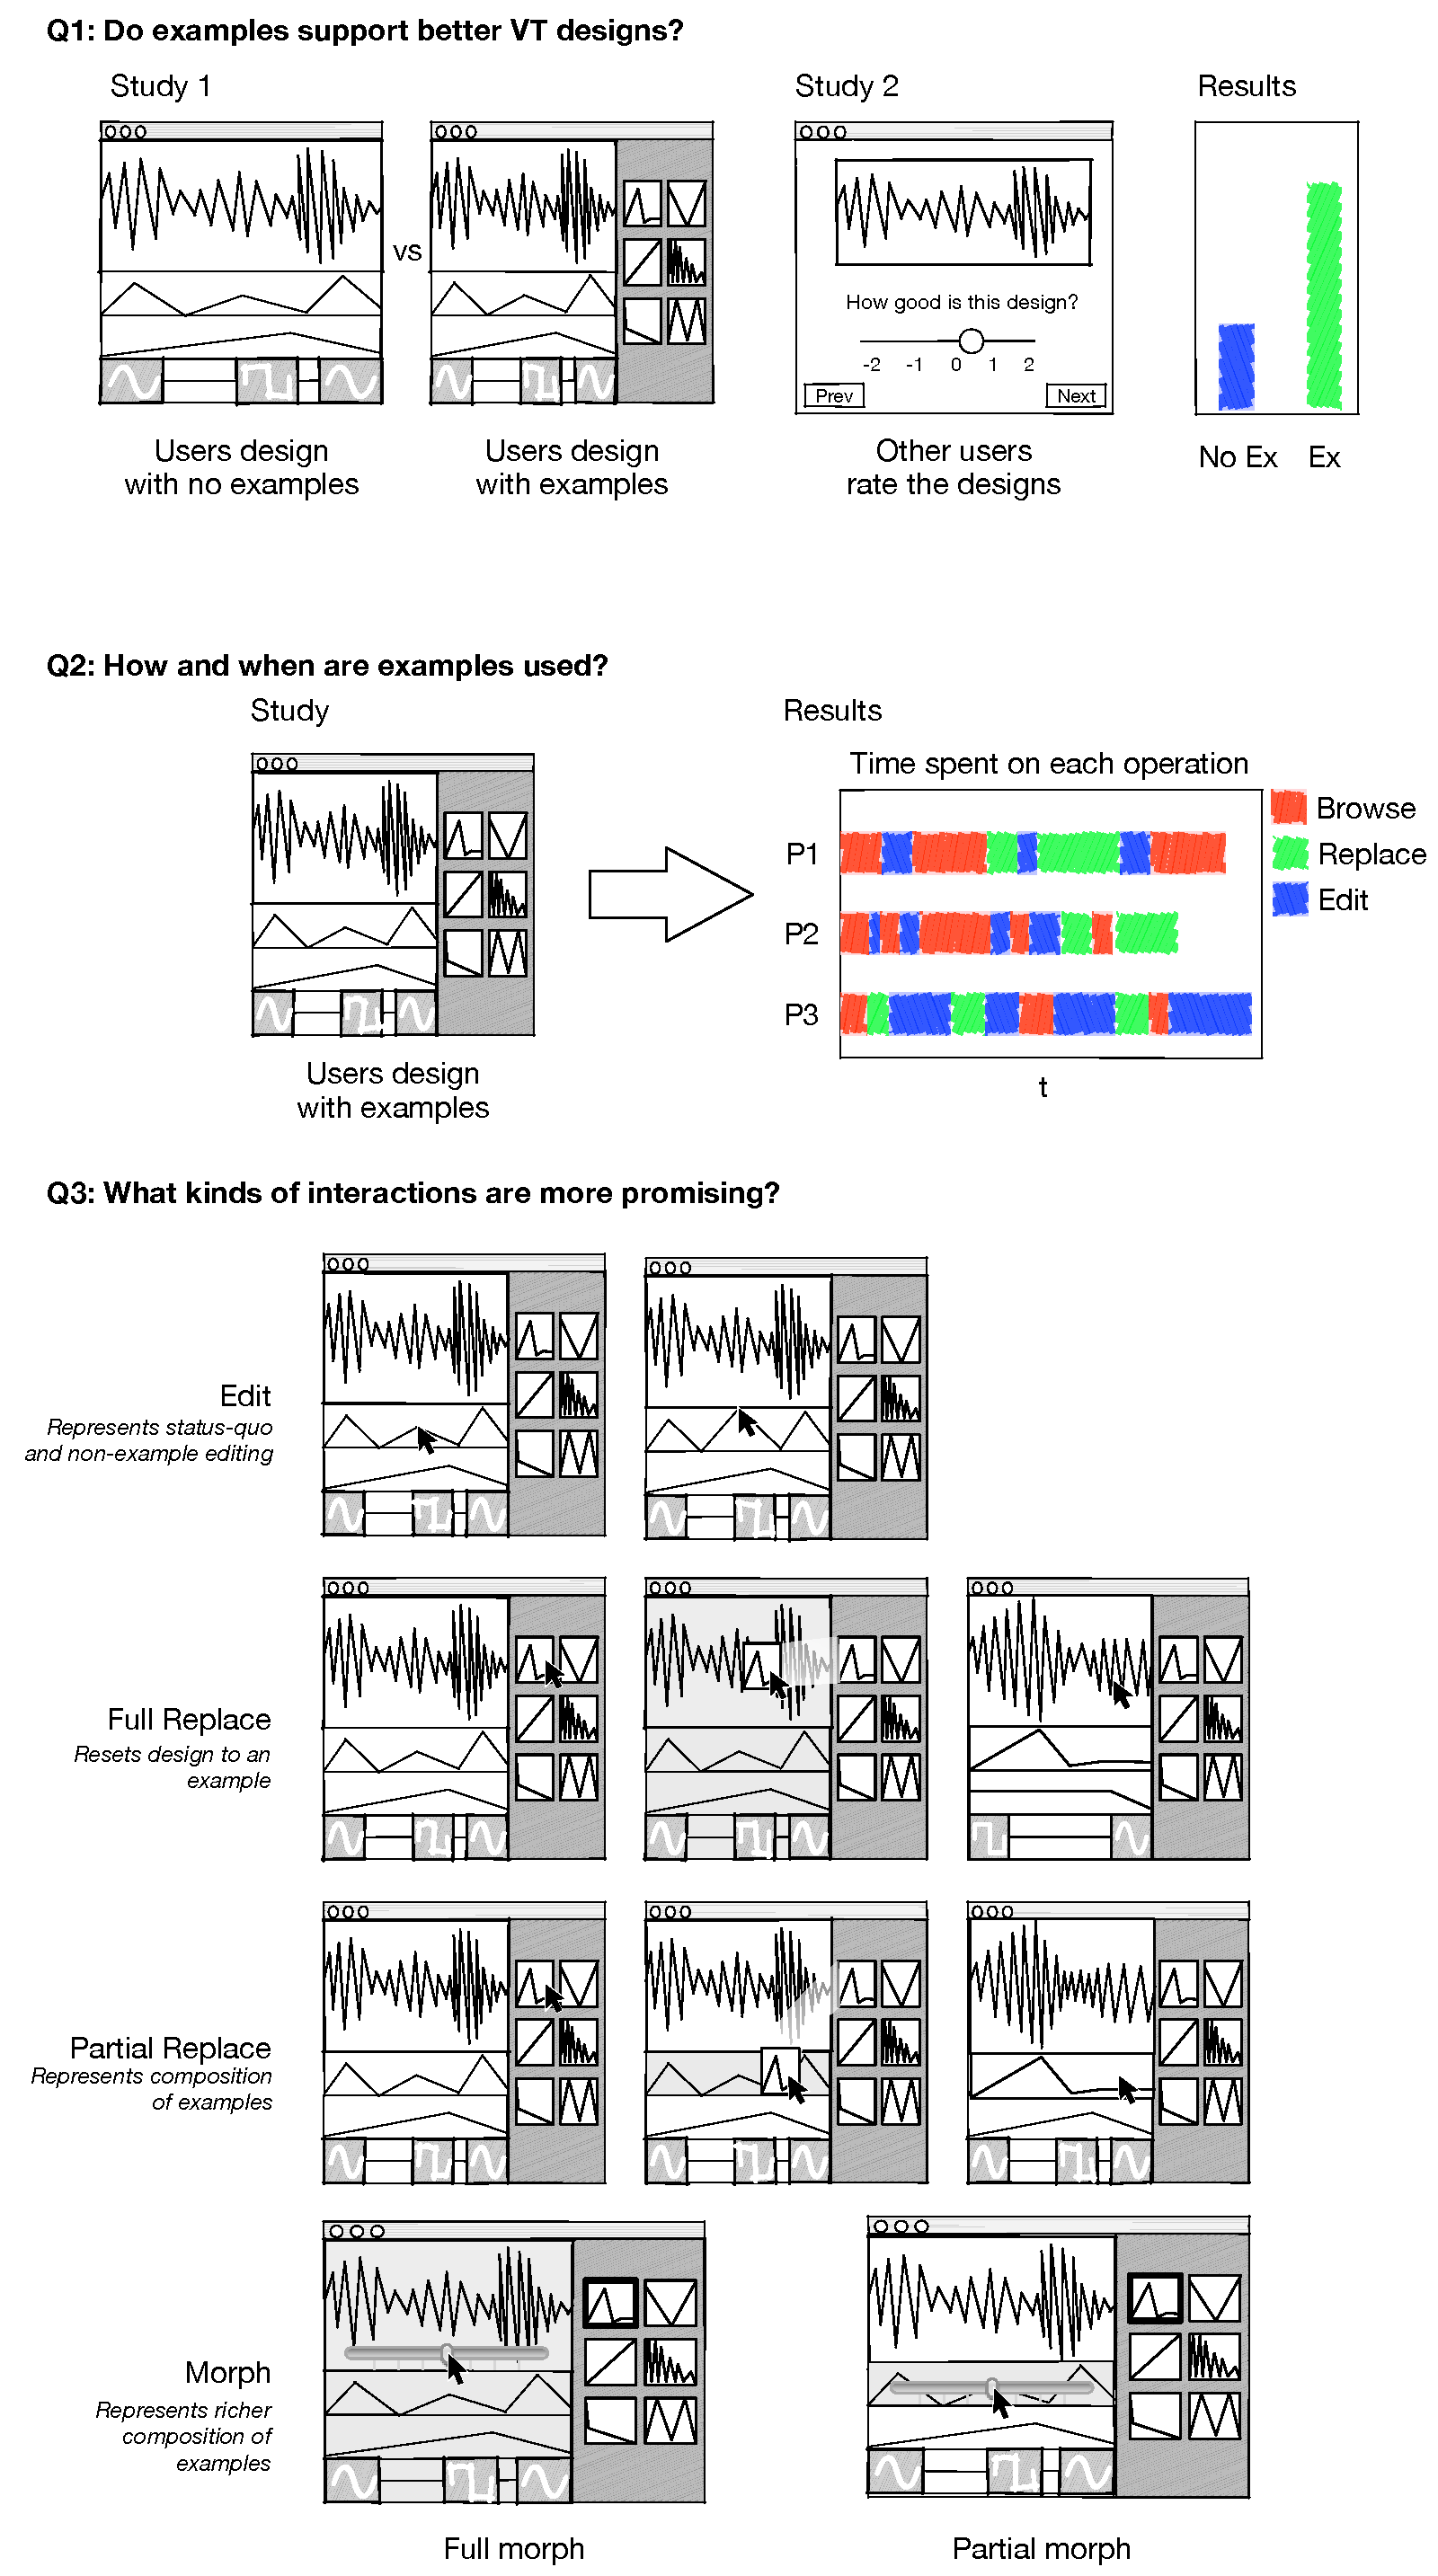
\includegraphics[width=0.7\textwidth, height=0.9\textheight]{DesignGalleryQuestions}

\caption{Phase II overview, split into research questions.}
\label{fig:macaron:phaseII:overview}
\end{center}
\end{figure}



%\begin{figure}[htbp]
%\begin{center}
%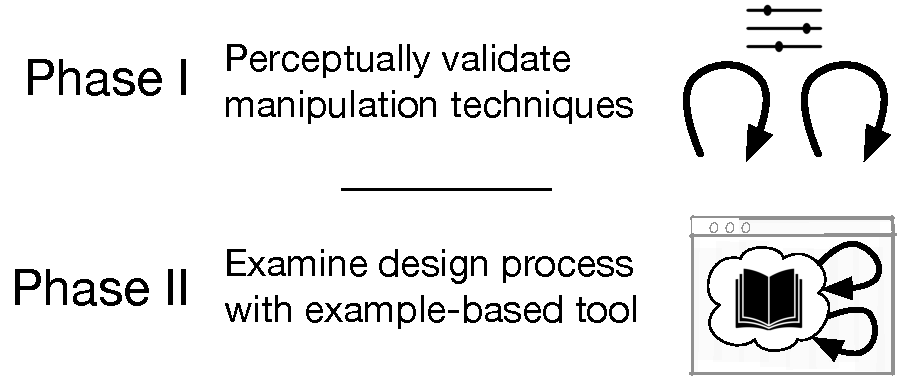
\includegraphics[width=0.8\textwidth]{ExamplesPhases}
%
%\caption{The two phases for the design gallery project.}
%\label{hapticexamples:phases}
%\end{center}
%\end{figure}



\endinput



\chapter{Synthesize: Generalization and Grounding}
\label{ch:haxd}


\begin{figure}[h] %  figure placement: here, top, bottom, or page
   \centering
   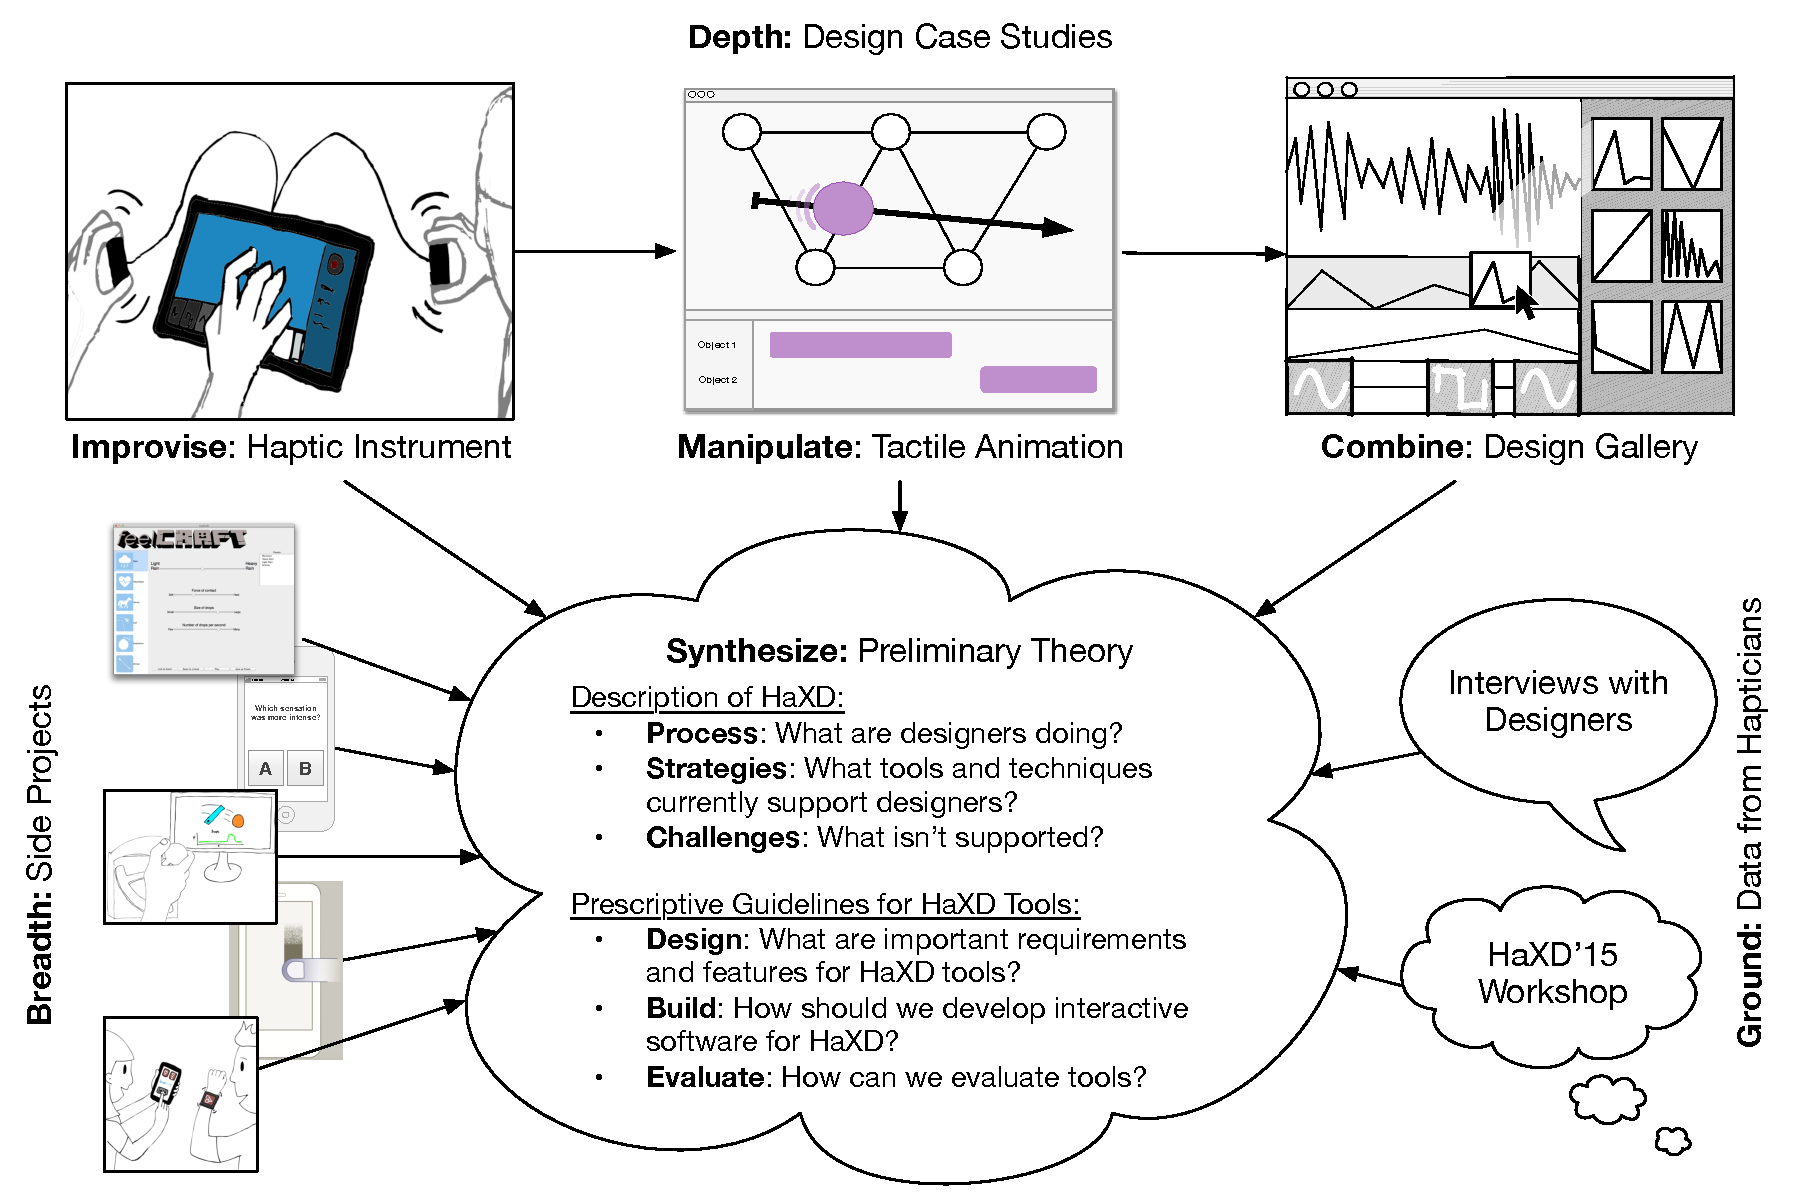
\includegraphics[width=0.7\textwidth]{HaXDTheoryOutline-2015-05-22} 
   \caption{Planned synthesis of data for a preliminary theory of haptic experience design.}
   \label{fig:haxd:theoryoutline}
\end{figure}


The three case studies provide rich but focused data on how to create vibrotactile (VT) experience design tools.
To complement these studies, I propose to gather information more broadly to generalize the haptic design process to other use cases and ground in haptician experience (\autoref{fig:haxd:theoryoutline}).
%from professional haptic designers.
In this way, my final contributions will draw from several sources: 
1) the three in-depth design studies,
%2) a literature survey of general design theories,
2) insight gathered from several side projects, and
3) two sets of grounded data: interviews with professional designers, and
%4) 
%informal interviews with peers at conferences, and 
a workshop at World Haptics `15.

Here, I describe the data collection process, then illustrate possible applications and forms for these contributions.
However, any resulting theory will be emergent from the data, and can take many forms.
To accomplish this in a principled way, I plan to use \emph{memoing} and \emph{constant comparison} \cite{Corbin2008}, looking for common threads between data and double-checking conclusions as new theoretical developments appear.
%This will be guided with a goal: to characterize haptic experience design, especially any features that are unique to this unique class of technological experiences.
This theory will also draw from a literature review of design theory, summarized in this document's related work section.
%This will provide information about non-haptic design disciplines and general theory of design to help frame our inquiry.




%%%%%%%%%%%%%%%%
%
% Section: Data Collection
%
%%%%%%%%%%%%%%%%
\section{Data Collection}
In this section, I list the different sources I intend to use to collect data for theory design.

\subsection{Vibrotactile design case studies}
Each of the  design case studies previously described investigates a specific user group working on a specific VT device with a specific software tool.
Through my experience of gathering requirements, creating tools (through design and development), and evaluating them, I will have first-hand knowledge of supporting aspects of VT sensation design.
Each also produces a small vignette of haptic design in action, giving us glimpses of the design process.

\subsection{Side projects}
In addition to the three design case studies that form this proposal, several side-projects are planned or underway as collaborative efforts.
In these side-projects, I take an organizational or supervisory role, often as summer projects conducted by undergraduates.

\begin{description}
	\item[FeelCraft and Feel Messenger] are collaborations with Disney Research members Ali Israr and Siyan Zhao, looking at distributing and customizing haptic effects in a consumer setting with low-fidelity rumble motor devices.
	I take a haptic designer role to gain a personal understanding of the process, and a software engineer role to understand relevant architectures. % for distributing haptic media.

	\item[CyberHap] is a collaboration between UBC and Stanford looking at force-feedback devices in education; a large team is involved with undergraduate Gordon Minaker leading development of a teaching interface since February 2015, co-supervised by PI Dr. Karon MacLean and me.
%	I co-supervise Gordon with PI Dr. Karon MacLean in this project looking at force-feedback devices in an education setting.
	
	\item[CuddleBit] is a project inspired by the Haptic Creature and CuddleBot project. A small, breathing and vibrating robot will be designed along with a behaviour prototyping tool in summer 2015.
	I supervise undergraduate Paul Bucci in this project exploring multiple modalities and potential for receiving input through a sensor.

	\item[HapTurk] is a collaboration with PhD candidate Hasti Seifi on different techniques to crowdsource feedback on VT icons. Master's student Salma Kashani and undergraduate Matthew Chun are developing visualizations and low-fidelity VT icons during summer 2015.
%	This project looks at a formal mechanism for doing large-scale feedback, and tackles the problem of cross-device and cross-modal equivalency (can a sensation be rendered in some fidelity on both low- and high-fidelity devices?).

	\item[RoughSketch] is a painting application for the TPad Phone, a variable-friction mobile device, for the World Haptics 2015 Student Innovation Challenge. Undergraduates Brenna Li, Paul Bucci, and Gordon Minaker are all fellow team members. Variable friction is a significant contrast to VT sensations as it is intrinsically connected to input: no sensation can be felt without active movement by the user.
\end{description}



\subsection{Grounded Data}
A corpus of interviews with professional haptic designers has already been collected by UBC alumni Colin Swindells during his PhD, but has never been published.
I will analyze these interviews to further ground our findings with real-world haptic designers.

To complement this %, and because professional haptic designers are rare and difficult to find,
we turn to the research community who do design as part of their work.
The planned Workshop on Haptic Experience Design (http://oliverschneider.ca/HaXD) at World Haptics 2015 will also provide a data source.
At this workshop, 4 experts of haptic experience design will speak, participants will reveal their own design challenges in a brainstorming activity, and the ensuing panel discussion should help illuminate practices and paths for future work.

%%%%%%%%%%%%%%%%
%
% Section: Possible Format
%
%%%%%%%%%%%%%%%%
\section{Possible Format}
While the theory can take many forms, I hope to characterize haptic experience design and contrast it with other design fields, especially graphic and audio design.
I hope to find both descriptive and prescriptive results, including current practices, an identification of challenges uniquely facing haptic designers, and guidelines for designers and developers of haptic design support tools.

\subsection{Descriptive Contributions: HaXD Process as Requirements}
My first goal is to describe the \textbf{processes} employed by haptic designers.
This could manifest, for example, as a catalogue of 
existing haptic design tools,
appropriated tools (e.g., using a sound editor to create VT icons),
techniques (e.g., design philosophies like Haptic Sketching),
resources (e.g., libraries and APIs),
platforms (what devices designers are using),
practices in haptics education (undergraduate or graduate level courses),
and tasks undertaken by haptic designers.

For example, to share of haptic experiences, haptic designers create demos
to spread awareness of haptic research and gain feedback from peers.
%One colleague, upon being introduced to the Haptics Symposium conference, said that the haptics community gets demos right.
This is so ingrained into the culture of haptic research that recently a demo-only conference was launched: Asia Haptics.

Once collecting a description of current practices, I expect we might be able to identify \textbf{challenges} and \textbf{strategies} to addressing those strategies, including the ecosystem of available tools: what is working well, and what is broken.
Using our example of collaboration and demos, we might see that in-person demos are effective, but
remote collaboration or asynchronous sharing is challenging. %, but could offer more frequent collaboration between designers.
Available tools include videos and visualizations of demos to explain concepts in lieu of the demo itself.
%Other challenges might include the great variety of different devices, non-haptic tools appropriated for haptic design, the implementation complexity of dealing with hardware, low-level software, and application logic simultaneously, or the strong influence of other modalities (vision, hearing) on perceived touch sensations.

\subsection{Prescriptive Contributions: Guidelines for HaXD Software Tools}
After describing HaXD as a set of requirements, I will then develop guidelines for how to built supportive interactive software tools.
Right now, I plan to organize this into three aspects: how to \textbf{design} tools, including important features relevant to different stages of HaXD; how to \textbf{build} tools, including relevant software architectures and ways to address technical challenges; and how to \textbf{evaluate} tools, methods to capture designer experience and inform future design.

Hypothetical use cases might best explain this contribution.
One examples is using these guidelines for knowledge transfer to industry.
I could use these guidelines to advise or create design software for companies developing haptic hardware platforms (such as the TPad team and UltraHaptics) or software platforms (such as Immersion and Phidgets), bridging the gap from research to industry application.
Another example could be dissemination through haptics education.
Developing a module for a haptic design course, such as CPSC 543, is an accessible way to encapsulate and test these ideas.
This could also manifest in a multi-day workshop, similar to Camille Moussette's Haptic Sketching workshops, to validate ideas at different institutions.



\section{Deliverables and Risk}
There are two expected deliverables from this theory development.
First, the HaXD'15 workshop on Haptic Experience design is planned, piloted, and scheduled for World Haptics in June, 2015. 
To get the most out of this workshop, photographs and notes will be recorded.
Afterwards, a very small digest piece debriefing the workshop is planned in winter 2016; this may be submitted on its own as an short paper if an appropriate venue is available (e.g., a special journal issue similar to \cite{Jones2014}), or subsumed into the second deliverable.

The second deliverable is a retrospective piece on our findings from all the data sources found here, but with a focus on data from haptic designer interviews.
This interview data has already been collected by UBC alumnus Colin Swindells.
I plan to digest and analyze those interviews in winter 2016 to generate requirements grounded in designer experience.
This will likely be combined with synthesized findings from the three design studies and several side projects.
To mitigate risk, we can combine interview findings to a greater or lesser extent with other data sources.
If the interviews have a great deal of information, they could be a valuable contribution on their own.
If not, I expect them to supplement our other data sources.
This document will likely be submitted as a full paper to a peer-reviewed conference or journal.

Within each project, we mitigate risk through strategic planning and study design;
many of these projects do not have to be successful to provide input.
For example, HapTurk may never actually be deployed, but could still articulate the challenge of a large-scale, remote haptic user study.
In addition,
risk is partially managed through sheer attrition: one or two side projects or data sources could provide limited feedback and we would still have a diverse set of information. 
However, I will note that initial investigation has already been useful.

%
%To ground our other findings with our target end users, and identify challenges that may not emerge from the literature alone.
%The goal is to develop an initial proposed theory of haptic experience design from multiple sources, which characterizes the unique process that can or could support designers.
%I plan to gather information from a variety of sources, including interviews with professional designers, informal interviews with peers during conferences, and the literature.


%The main source of data will be from interviews with professional designers, several of which have been collected already by researcher Colin Swindells.
%These will be analyzed using qualitative techniques like grounded theory and phenomenology \cite{Creswell2013, Moustakas1994}.
%
%A second source of data will be reflection on our own projects and those of our peers and collaborators.
%
%
%Currently, much of the literature review has already been conducted for this document, 
%





%% KM - for comments
%\newcommand{\inlinecomment}[3][]{$\lceil$\textbf{#1}~\textit{\textcolor{#2}{#3}}$\rfloor$}
%\definecolor{DarkGreen}{rgb}{0.0, 0.5, 0.0}
%\definecolor{DarkRed}{rgb}{0.7, 0.2, 0.2}
%\definecolor{DarkOrange}{rgb}{1, 0.5, 0}
%\definecolor{Orange}{rgb}{1, 0.75, 0}
%\newcommand{\kmC}[1]{\noindent \inlinecomment[KM]{DarkGreen}{#1}}
%\newcommand{\kmE}[1]{\textcolor{DarkRed}{#1}}
%\newcommand{\osC}[1]{\noindent \inlinecomment[OS]{Orange}{#1}}
%%\newcommand{\osC}[1]{}
%\newcommand{\osE}[1]{\textcolor{DarkOrange}{#1}}
%
%%Organization commands
%\newcommand{\inlineHeading}[1]{\emph{#1} --}
%
%%\newcounter{pathwayCounter}
%\newcommand{\challenge}[1]{\textbf{Pathway: #1} --}
%
%
%Although haptic technologies have become commonplace in end-user experiences, there are still few established processes to guide designers, who face special challenges that arise out of the relative youth of the field and from qualities intrinsic to the sense of touch.
%Design guidelines, toolkits, and authoring interfaces exist as disparate pieces of knowledge rather than a unified perspective, 
%hobbling the creativity and efficiency needed to create new haptic experiences. 
%In this paper, we assemble key elements of the haptic design process and its
%needs
%into a generalized
% framework and vocabulary, 
%to promote
% a more fluid, extendable, and transferrable understanding of the practice, 
%guide development of effective tools, and 
%promote a discourse around both. 
%We begin with haptic versions of three primary
% design activities identified in
% design theory, creativity support tools, and other fields of design: problem preparation, hands-on design, and collaboration.
%These activities form a framework by which we can organize the haptic design literature and our own experience 
%into specifically defined
%pathways for design, identifying areas for future research and implications for tool development.
%
%
%
%
%\begin{table*}
%\caption{Design Activities, Sub-Activities, and Pathways Synthesized from the Literature}
%\label{tab:designactivities}
%
%%
%%
%%% Old version - horizontally laid out
%%
%%\begin{center}
%%	\begin{tabular}{|c|c|c|c|c|c|c|c|c|}
%%	\hline
%%		
%%		
%%	\multicolumn{3}{|c|}{\bf Problem Preparation (\Cref{sec:problempreparation}) }
%%		& \multicolumn{3}{|c|}{\bf Hands-on-Design (\Cref{sec:handsondesign})}
%%		& \multicolumn{3}{|c|}{\bf Collaboration (\Cref{sec:collaboration})} \\
%%		
%%		\multicolumn{3}{|c|}{\emph{Use the Designer's Experience}}
%%		& \multicolumn{3}{|c|}{\emph{Navigate a Design Space}}
%%		& \multicolumn{3}{|c|}{\emph{Design together}} \\
%%		
%%	\hline
%%		
%%	Framing
%%		& Repertoire
%%		& Examples
%%	& Ideation
%%		& Evaluation
%%		& Sketching
%%	& Relate
%%		& Feedback
%%		& Donate \\
%%		
%%	%sub-activities
%%	\emph{Defining}
%%		& \emph{Internal}
%%		& \emph{External}
%%	& \emph{Generation}
%%		& \emph{Filtering}
%%		& \emph{Rapid, flexible,}
%%	& \emph{Informal talks}
%%		& \emph{Formal studies}
%%		& \emph{Dissemination} \\
%%		
%%	\emph{the problem}
%%		& \emph{experience}
%%		& \emph{resources}
%%	& \emph{of ideas}
%%		& \emph{of ideas}
%%		& \emph{ambiguous notation}
%%	& \emph{with peers, mentors}
%%		& \emph{with users}
%%		& \emph{to community} \\
%%		
%%%	\hline	
%%%	%Challenges
%%%	\emph{Flexible interfaces,}
%%%		& \emph{Accessible}
%%%		& \emph{Example}
%%%	& \multicolumn{2}{|c|}{Support multiple}
%%%		& \emph{Support ambiguity,}
%%%	& \multicolumn{3}{|c|}{Challenge: \emph{investigate asynchronous,}} \\
%%%		
%%%	\emph{multiple views}
%%%		& \emph{knowledge}
%%%		& \emph{management}
%%%	& \multicolumn{2}{|c|}{parallel designs}
%%%		& \emph{commenting, abstraction}
%%%	& \multicolumn{3}{|c|}{ \emph{distributed collaboration}} \\	
%%		
%%	\hline
%%	\end{tabular}
%%\end{center}
%%\end{table*}
%%
%
%
%\begin{center}
%	\begin{tabular}{lll}
%	\toprule
%		
%
%%	\rowcolor [gray]{.8}
%	\textbf{Activity}
%		& \textbf{Sub-Activity}
%		& \textbf{Pathways for Design}
%		\\
%	\midrule
%	
%	\multirow{3}{1.7in}{\textbf{Problem Preparation (\Cref{sec:problempreparation})} \emph {Use the Designer's Experience}}
%		& Framing -- Defining the problem
%		& Flexible interfaces, multiple views, powerful language
%		\\
%	\cmidrule{2-3}
%		& Repertoire -- Internal experience
%		& Task-based knowledge source
%		\\
%	\cmidrule{2-3}
%		& Examples -- External resources
%		& Manage examples: capture, find, access, transform
%		\\
%	\midrule
%	
%	\multirow{3}{1.7in}{\textbf{Hands-on Design (\Cref{sec:handsondesign})} \emph {Navigate a Design Space}}
%		& Ideation -- Generate ideas
%		& \multirow{2}{*}{Explore multiple design candidates in parallel}
%		\\
%	\cmidrule{2-2}
%		& Evaluation -- Filter ideas
%		&
%		\\
%	\cmidrule{2-3}
%		& Sketching -- Rapid, flexible, ambiguous notation
%		& Support speed, ambiguity, commenting, abstraction
%		\\
%	\midrule
%	
%	
%	\multirow{3}{1.5in}{\textbf{Collaboration (\Cref{sec:collaboration})} \emph {Design Together}}
%		& Relate -- Informal talks with peers, mentors
%		& \multirow{3}{*}{Explore asynchronous and distributed interactions}
%		\\
%	\cmidrule{2-2}
%		& Feedback -- Formal studies with users
%		&
%		\\
%	\cmidrule{2-2}
%		& Donate -- Dissemination to community
%		&
%		\\
%	
%		
%%	\multicolumn{3}{|c|}) }
%%		& \multicolumn{3}{|c|}{\bf Hands-on-Design (\Cref{sec:handsondesign})}
%%		& \multicolumn{3}{|c|}{\bf Collaboration (\Cref{sec:collaboration})} \\
%%		
%%		\multicolumn{3}{|c|}{\emph{Use the Designer's Experience}}
%%		& \multicolumn{3}{|c|}{\emph{Navigate a Design Space}}
%%		& \multicolumn{3}{|c|}{\emph{Design together}} \\
%%		
%%	\hline
%%		
%%	Framing
%%		& Repertoire
%%		& Examples
%%	& Ideation
%%		& Evaluation
%%		& Sketching
%%	& Relate
%%		& Feedback
%%		& Donate \\
%%		
%%	%sub-activities
%%	\emph{Defining}
%%		& \emph{Internal}
%%		& \emph{External}
%%	& \emph{Generation}
%%		& \emph{Filtering}
%%		& \emph{Rapid, flexible,}
%%	& \emph{Informal talks}
%%		& \emph{Formal studies}
%%		& \emph{Dissemination} \\
%%		
%%	\emph{the problem}
%%		& \emph{experience}
%%		& \emph{resources}
%%	& \emph{of ideas}
%%		& \emph{of ideas}
%%		& \emph{ambiguous notation}
%%	& \emph{with peers, mentors}
%%		& \emph{with users}
%%		& \emph{to community} \\
%		
%%	\hline	
%%	%Challenges
%%	\emph{Flexible interfaces,}
%%		& \emph{Accessible}
%%		& \emph{Example}
%%	& \multicolumn{2}{|c|}{Support multiple}
%%		& \emph{Support ambiguity,}
%%	& \multicolumn{3}{|c|}{Challenge: \emph{investigate asynchronous,}} \\
%%		
%%	\emph{multiple views}
%%		& \emph{knowledge}
%%		& \emph{management}
%%	& \multicolumn{2}{|c|}{parallel designs}
%%		& \emph{commenting, abstraction}
%%	& \multicolumn{3}{|c|}{ \emph{distributed collaboration}} \\	
%		
%	\bottomrule
%	\end{tabular}
%\end{center}
%\end{table*}
%
%
%
%
%%%%%%%%%%%%%%%%%%%%%%%%%%%%%%%%%%%%%%%%%%%%%%%%%%%%%%%%%%%%%%%%%%%%%%%%%%%%%%%%%
%\section{Introduction}
%Haptic technology has become a 
%standard ingredient of user interactions with technology, with the potential to add engagement to media experiences \cite{Modhrain2001, Danieau2014} and ``calm'' everyday interactions \cite{MacLean2009}.
%% No longer restricted to research labs or theme park rides, 
%Carefully designed and expressive haptic feedback is finding its way into commercial devices, most recently the Apple Watch (www.apple.com/watch).
%
%
%
%\begin{figure}[tbp] %  figure placement: here, top, bottom, or page
%	\centering
%	\begin{subfigure}[b]{0.23\textwidth}
%		   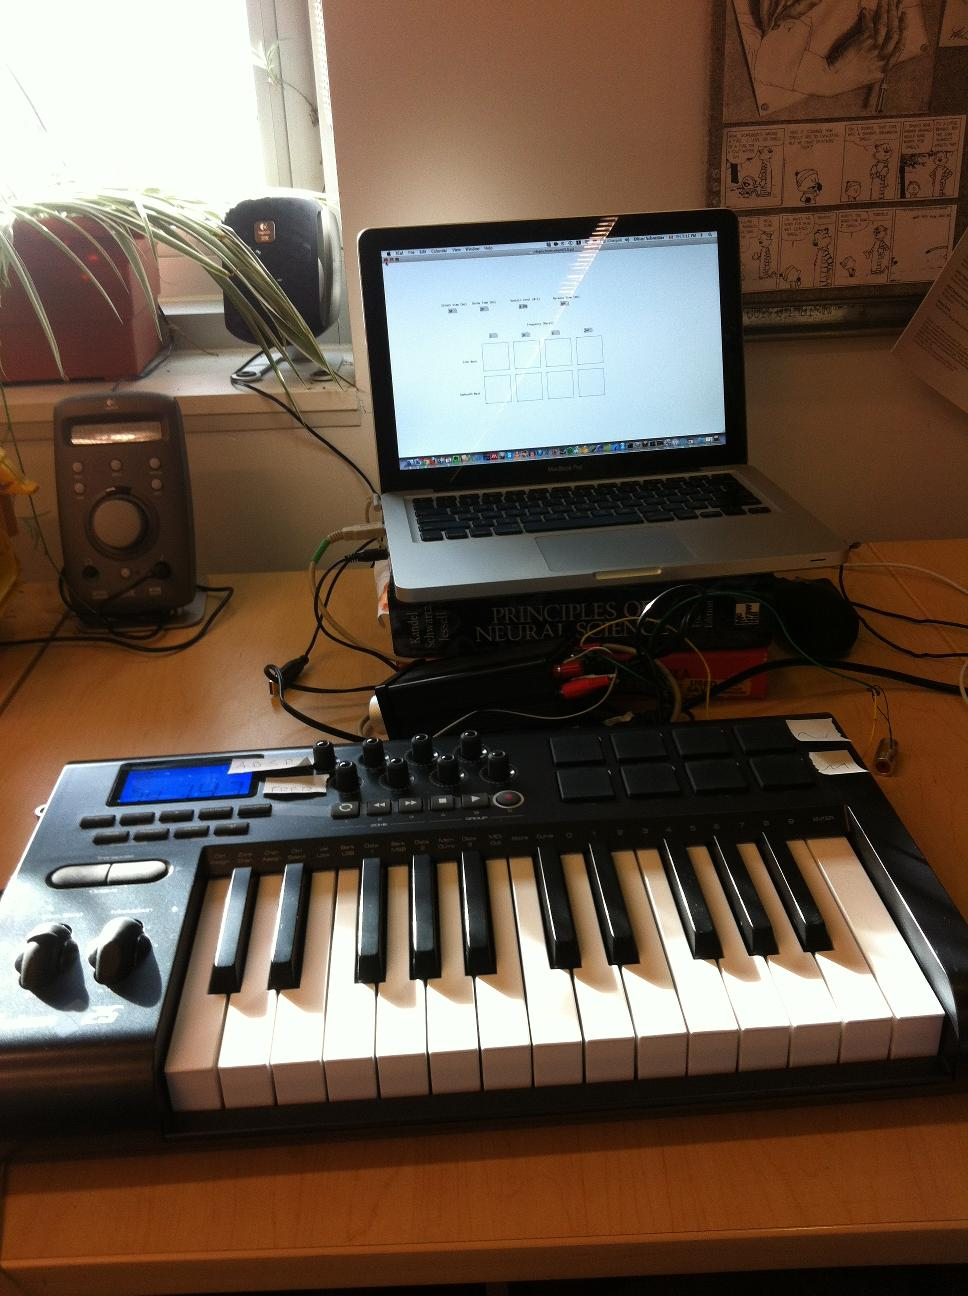
\includegraphics[height=2.3in]{figures/HIVE-photo} 
%		   \caption{Early hardware sketch}
%		   \label{fig:example:hardware}
%	\end{subfigure}
%	\quad
%	\begin{subfigure}[b]{0.22\textwidth}
%		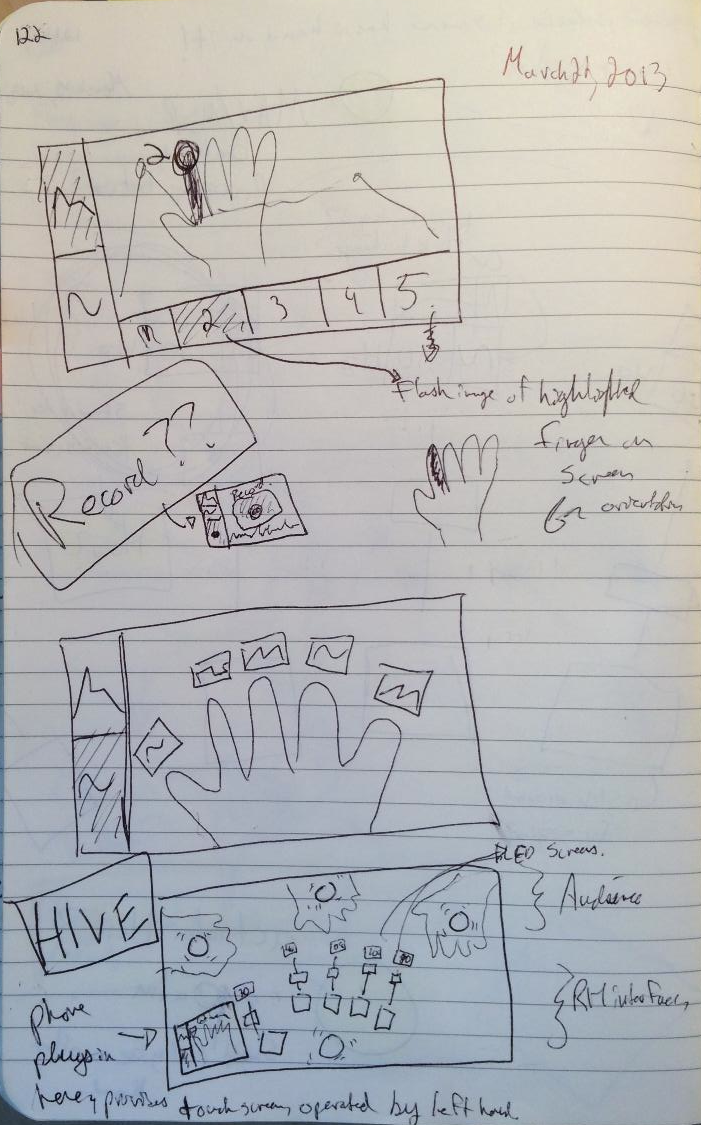
\includegraphics[height=2.3in]{figures/mHIVE-earlysketch-photo-cropped} 
%		\caption{Early paper sketch}
%		\label{fig:example:paper}
%	\end{subfigure}
%	\caption{Early sketches for mHIVE \cite{Schneider2014} in hardware (a) and on paper (b), showing a \emph{framed} approach (instrument metaphor), inspiration from the designer's \emph{repertoire} (musical experience), and extension of \emph{examples} (dials and buttons adapted from the keyboard).}
%	 \label{fig:example}
%\end{figure}
%
%
%% Despite this growth, 
%Nevertheless, there is no established process for haptic experience design (``HaXD").
%% (HaXD) %OS: We never reuse this, but may want to in future drafts
%% has no established design process.
%% One culprit is the small and fragmented user base:
%Culprits abound. The user base is small and fragmented:
%professional haptic designers are still rare, often share engineering or scientific duties, and tend to be sequestered in companies whose business needs preclude broader interactions % with other designers.
%and complicate observation of design practices by researchers.
%%\kmE{They lack both training in an articulated user-experience design approach, and an interlinked community through which they can consolidate vocabulary and share best practices.}
%It is difficult to translate guidelines from other fields, in absence of analogies to % graphic design's 
%colour % theory 
%or musical theory. % for touch.
%Designing for the sense of touch entails % brings intrinsic design challenges, such as  %as it involves 
%hard-to-prototype hardware and context-sensitive perception~\cite{Hayward2008}.
%
%%However, when attempting to get that ineffable quality of getting something to ``feel right" in a given context, a robust design process can help when prescriptive guidelines fail.
%
%Recently, design thinking applied to haptics \cite{Moussette2012} has added to the literature on HaXD process \cite{Swindells2006}.
%Toolkits \cite{Minamizawa2012,Ledo2012}, effect libraries \cite{Israr2014},  collaborative software \cite{Ruthenbeck2014,Cha2009} and interfaces themselves \cite{Schneider2014} ease production of haptic \emph{effects}.
%However, a systematic, convergent procedure by which haptic \textit{experiences} can be developed
%to meet specific requirements -- which themselves may be hard to articulate -- is elusive, % not well defined, 
%with previous work providing only % isolated elements. % 
%pieces of the puzzle.
%
%In this paper, we aim to situate
%haptic design tasks in a common framework.
%Synthesizing insights from design and creativity literature, we describe
% three critical activities conducted during many types of design: 
% \textit{problem preparation}, \textit{hands-on design}, and \textit{collaboration}, each with
% sub-activities.
%We discuss each in the haptic context to discover what activities are supported and which are not,
%with examples drawn from literature and our personal experience as designers and observers of other designers.
%This design lens
%reveals not only a process, but pathways for more focused investigation, informing the creation of HaXD support tools.
%
%
%
%%\inlineHeading{Design Activities}
%
%
%%\begin{table}
%%\caption{Problem Preparation Sub-Activities}
%%\label{tab:problem:preparation}
%%\begin{center}
%%	\begin{tabular}{|l|p{2cm}|p{2cm}|p{2cm}|}
%%	\hline
%%		&Description	&Haptics so far	& Haptics next	\\
%%	
%%	
%%%	\hline
%%%	\textbf{Problem Preparation}	&	&	&	\\
%%	
%%		\hline
%%		\emph{Framing}
%%			& transforming the problem into a manageable form
%%			& Ongoing investigation of haptic language, perceptual dimensions
%%			& Flexible, adaptable tools; multiple views	\\
%%
%%		\hline
%%		\emph{Repertoire}
%%			& building the designer's internal experience
%%			& Haptics education (e.g., HapKit,  Twiddler), DIY haptics, haptic illusions
%%			& Handbook, wiki, or other more elaborate compendium of knowledge	\\
%%		\hline
%%		\emph{Examples}
%%			& Drawing from external resources and designs
%%			& Haptic camera, libraries (Immersion, Upenn, FeelEffects), haptic search engine
%%			& Capture \& upload, find (search/explore/visualize), use (design galleries, editable data types)	\\
%%	\hline
%%	\end{tabular}
%%\end{center}
%%\end{table}
%
%
%
%%\subsection{Challenge: Difficult Problem Framing}
%%The CHALLENGES (unfilled holes):
%%
%%1. Problem Gathering:
%%No Language, limited theory (framing)
%%Complex sense (hard to understand, need to be expert in multiple domains
%%) (repertoire+framing)
%%No language/theory
%%limited ways to capture, render, maintain examples
%
%
%\challenge{Multiple metaphors}
%Despite a steady progression of research on perception,
%there is no agreed upon language for working with haptics \cite{Obrist2013,Okamoto2013,Jansson-Boyd2011}.
%Most authoring tools have relied on fixed metaphors and devices, limiting \emph{framing}.
%Allowing  multiple metaphors or views on a haptic design is one way in which a designer can % would allow the designer to 
%reshape a problem to be easier to solve (reframe it so it matches their \emph{repertoire} or found \emph{examples}).
%Future authoring tools should pursue flexibility or improved abstractness.
%%Abstract metaphors could apply to multiple device classes, .
%
%%Examples:
%%?	Haptic Camera
%%?	Kuchenbecker?s haptic textures
%%?	Libraries
%%?	Feel Effects/FeelCraft
%%?	Ultrasound Examples from Keisuke Hasegawa?s HaptoMime at AsiaHaptics:
%%o	Tried a bunch of waveforms extracted from sound sources in the Komplete audio packagewith my own palm. It?s a pity that there was no systematic procedure to determine what waveform to pick up. My only advice is that it would be good and efficient to construct an experimental system which allows you to test many kinds of stimuli promptly at an early stage in y our researches.
%%?	Need examples from industry
%
%
%
%%\kmC{Isn't this a library not an education problem? SLC} % Not following the focus on haptics education here, as related to repertoire. Can you strengthen the connection? I thought this particular challenge would be more about how designers can capture, organize, find, reuse externally sourced inspiration and examples - essentially, the library problem. Education, and communication with one another, is an important but different challenge.}
%% That said, I am still fuzzy on distinction between repertoire and examples. They both need libraries, don't they? Because there are a lot of them, and the point is re-use. 
%\challenge{Task-based knowledge}
%To build their \emph{repertoire}, haptic designers must learn essential haptics concepts and begin solving relevant problems.
%Haptics courses \cite{Okamura2012, Jones2014} often provide a HaXD practitioner with initial experience.
%Brief, cogent outlines  of haptics knowledge (e.g., \cite{Hayward2007,MacLean2008,Hayward2008,Karam2013}) allow designers to expand their experience in an accessible way, and resources like EduHaptics (eduhaptics.org) link designers to content.
%However, knowledge is still framed with disparate perspectives. 
%The next step is to understand the low-level tasks conducted in HaXD.
%This would enable development of a more focused ``how-to" compendium of knowledge uniting perception, hardware, and software knowledge bases.
%%Ideally, this will link directly to HaXD tasks, but more research is needed to understand the .
%%, but still accessible, source of knowledge; a handbook of haptics knowledge that summarizes perceptual research, lists prominent examples of design, and guidelines for design and development.
%%This need not be a traditional handbook, but could be an online tool, such as a wiki or online course.
%%A proposed handbook might have more content internalized, structured to be handy and self contained, featuring design case studies.
%
%%\emph{Examples}
%\challenge{Manage examples}
%Currently, \emph{examples} exist in several libraries (e.g., \cite{Culbertson2014, Israr2014}), but capturing, organizing, accessing, and transforming them poses a greater challenge for haptic design than for more visually oriented, or even auditory, domains.
%%Excluding progress made by expanding these libraries in scale or in device support, there are key areas we can look for future progress.
%Capturing with a haptic camera  \cite{MacLean1996} is useful, but limited to that camera's target phenomenon.
%Integration of library uploads into authoring tools (e.g., as suggested in \cite{SchneiderAsiaHaptics2014}), would make it easier to grow a set of \emph{examples}.
%Visualizations, searching techniques (like a haptic search engine \cite{Adi2010,Hanamitsu2014}), and browsing techniques will facilitate access.
%%One demoer at a recent conference described his approach to create a tactile effect.
%%He tried waveforms extracted from sound sources in the Komplete audio package, stating ``It's a pity that there was no systematic procedure to determine what waveform to pick up" and wishing for a system to try stimuli at an early stage.
%%with my own palm. It?s a pity that there was no systematic procedure to determine what waveform to pick up. My only advice is that it would be good and efficient to construct an experimental system which allows you to test many kinds of stimuli promptly at an early stage in y our researches.
%%In haptics, we have already done some work on capturing examples, for example, the haptic camera \cite{MacLean1996}, or empirically gather libraries \cite{Culbertson2014}.
%% Some examples or templates are often shipped with toolkits (Verify!), and recently vibrotactile libraries have been developed: Immersion, Feel Effects, or the UPenn surface toolkit \cite{Culbertson2014}.
%%The haptic search engine (asia haptics) is one way of recalling examples.
%Finally, current \emph{examples} are static -- the designer chooses one and adds it to their application.
%%Novel techniques of using examples to create new designs.
%Open, manipulatable formats beyond parameters (like those in \cite{Ledo2012,Israr2014}) or through design galleries \cite{Lee2010a,Marks1997} is an exciting avenue to allow designers to work hands-on with \emph{examples}.
%
%%Originating in the graphics literature, design galleries provide a set of designs similar or different from your current design, letting users take interesting parameters and apply them to their design \cite{Marks1997}.
%%This idea has since been applied to other design fields like web design \cite{Lee2010a}.
%%Given the difficulty of framing with no fixed haptic parameters or language \cite{Jansson-Boyd2011}, example-based design could be a promising avenue for future design tools.
%%It's also been recommended that focusing on rapid prototyping can get around language barriers in haptics \cite{Fogg1998}.
%%To do this, we need to focus on hands-on design of haptics, the second major design activity.
%
%
%
%%Rapid iteration is essential for being able to think by doing; creativity support tools must have a low threshold, high ceiling, and wide walls: accessible to beginners, powerful for complete solutions, and support a wide range of explorations \cite{Resnick2008}.
%%A sketch can have many purposes, but is distinguished from a prototype by being more generative, less complete, and characteristic of earlier design \cite{Buxton2007}.
%
%
%
%
%%Donald Sch\"{o}n's seminal book, The Reactive Practitioner, describes the process of
%%learning skills to be one of reflection-in-action. That is, a pitcher in a baseball game must be able to find their groove. Through a process of subtle adjustment and experimentation, a pitcher adjusts her technique to fit the current, myriad conditions the wind, the current batter, the sun; the list goes on. This process is implicit, and often people find it impossible to articulate. Like the poor centipede, we sometimes find it difficult to realize that knowledge is embedded in our action, and in fact it can ruin our stride. Verbal overshadowing, articulating a wine's taste or a person's face, often weakens our memory unless we've been trained to verbalize those notions \cite{Schooler1990}. Similarly, a haptic designer must adapt to her design project to the current conditions.
%
%%Idea generation vs Idea evaluation. Sketching.
%
%
%%\begin{figure}[htbp] %  figure placement: here, top, bottom, or page
%%   \centering
%%   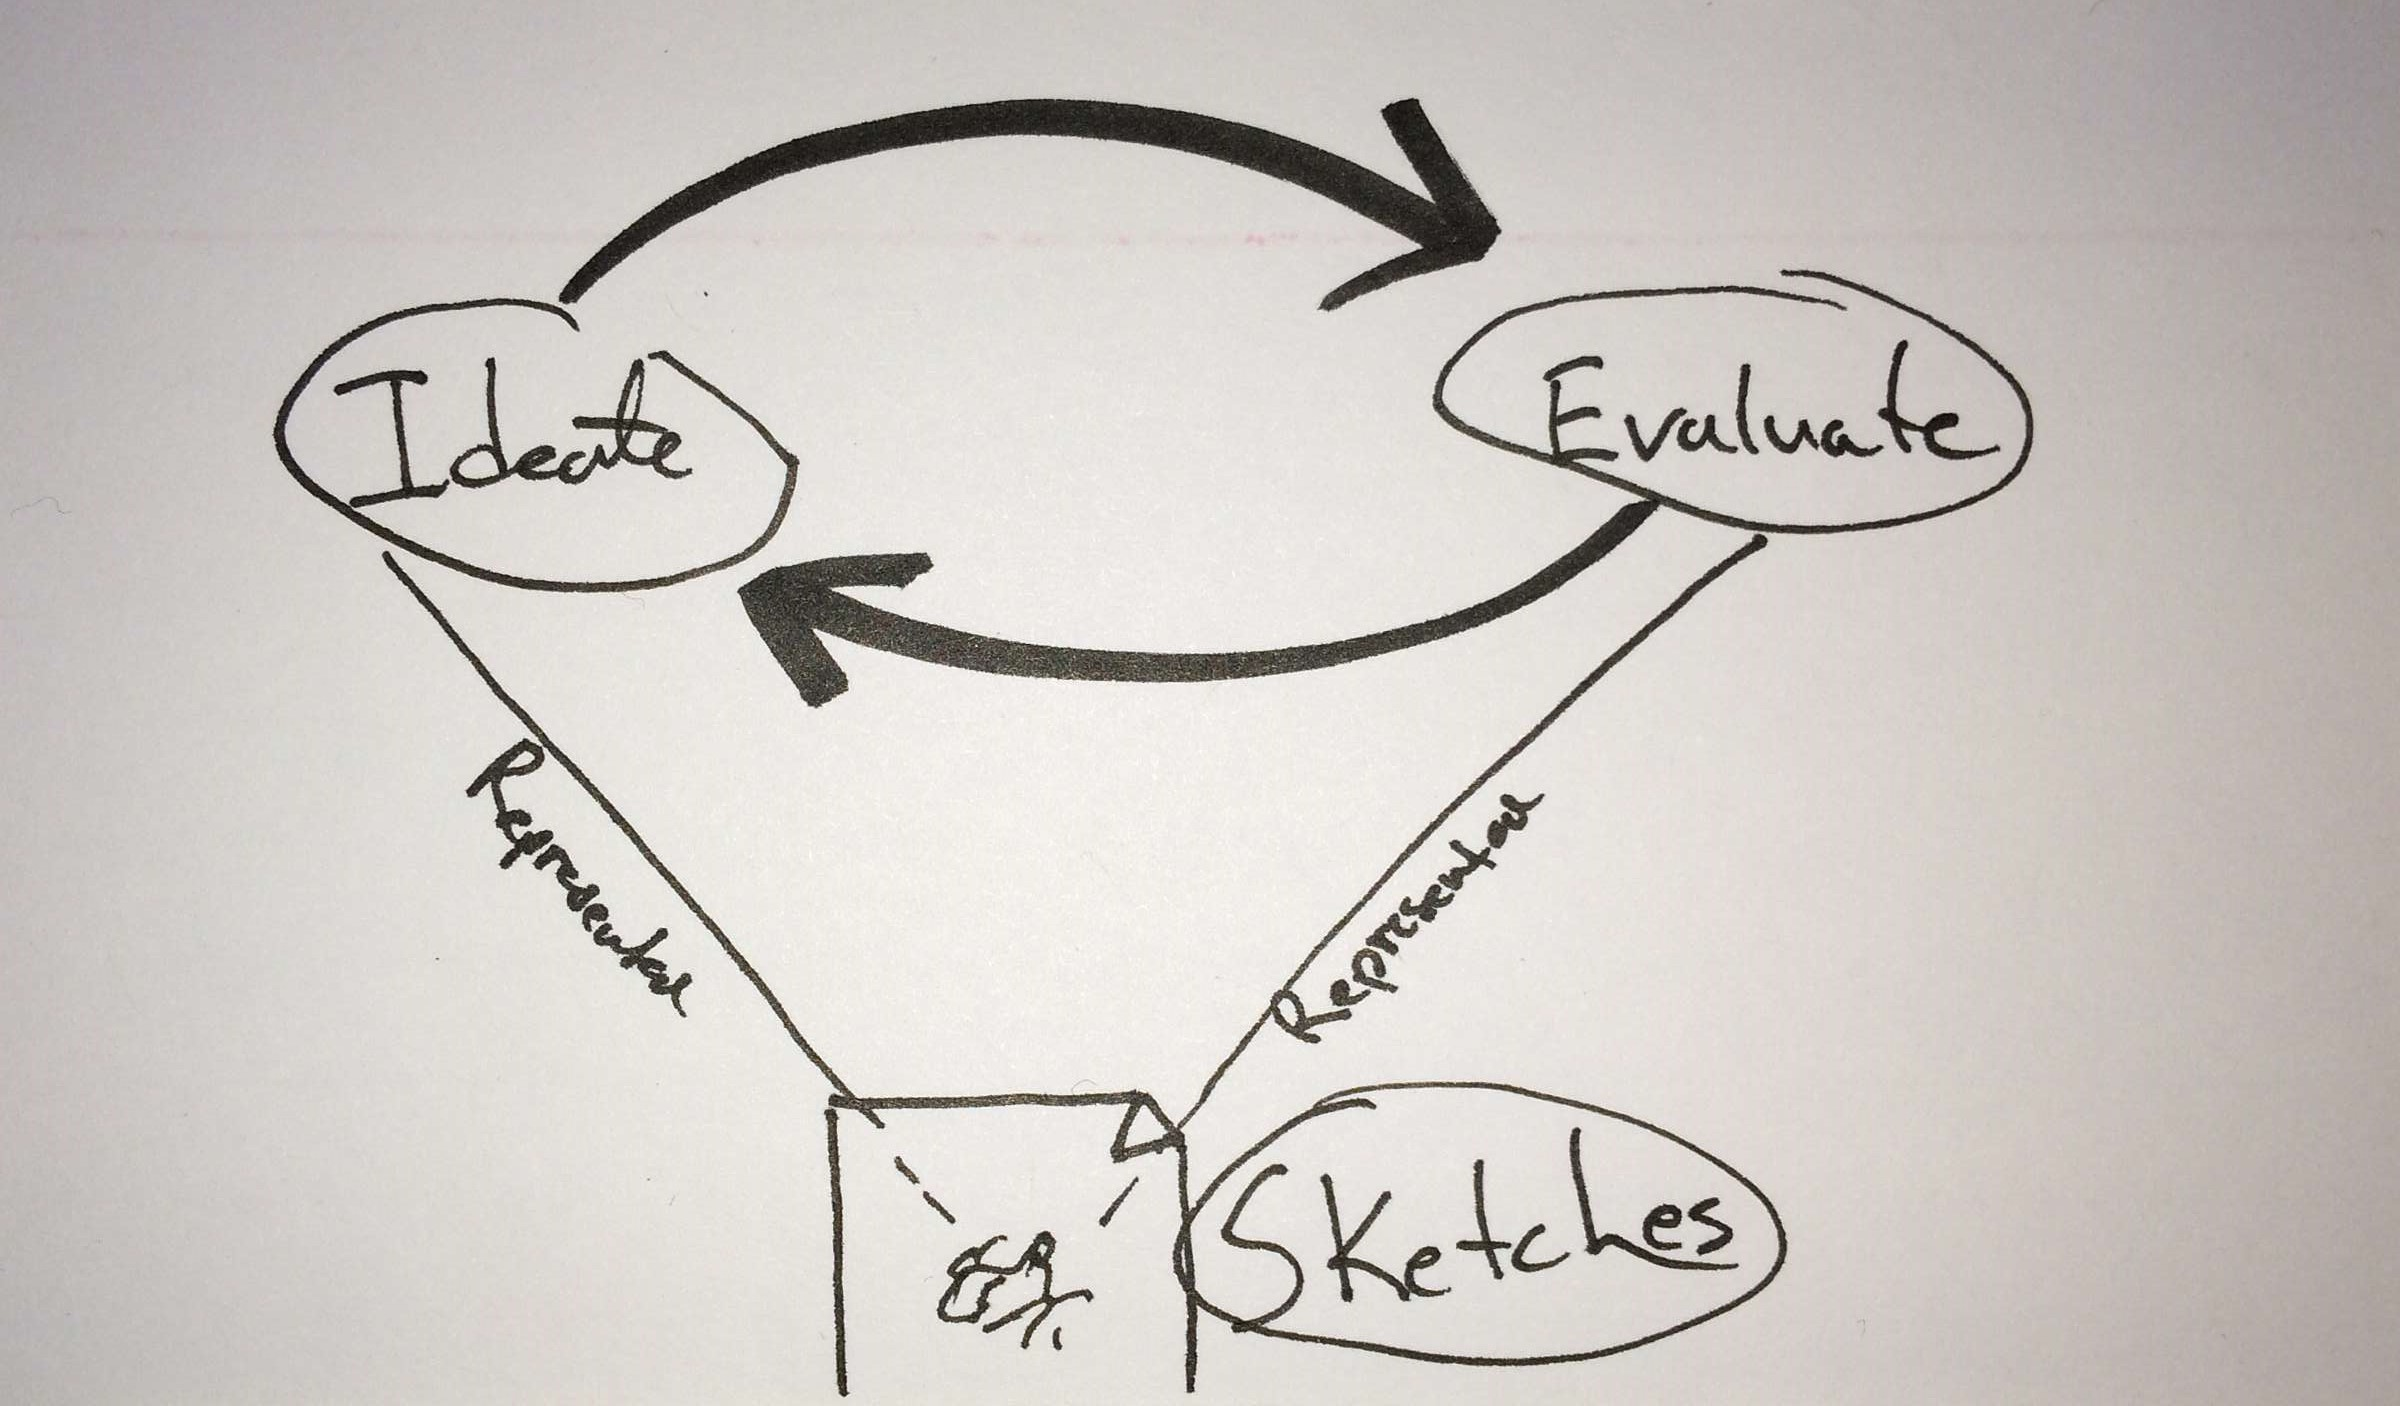
\includegraphics[width=0.48\textwidth]{figures/HandsOnDesignSubProcessesPlaceHolder} 
%%   \caption{Hands-on design sub-activities. Designers iterate between ideation and evaluation, representing this process through sketches.\textbf{(PLACEHOLDER)}}
%%   \label{fig:hands:on:sub:activities}
%%\end{figure}
%
%
%\challenge{Multiple, parallel designs}
%Ideation and evaluation are partially supported by existing tools.
%Parallel development of interfaces has been applied to physical UIs with Arduino \cite{Hartmann2008}.
%Brainstorming and techniques like A/B testing, comparing two designs side-by-side, have been employed in haptics design tools \cite{Swindells2014}.
%Rapid ideation and evaluation are also supported through better framing tools like design galleries, described in the previous section.
%
%\challenge{Ambiguity, commenting, \& ad-hoc use}
%%Haptic design suffers from slow iteration.
%%Developing a haptic sensation often requires custom hardware, software, and coordination between the two.
%%Further, other senses must be considered, meaning a full stack of hardware to high-level GUI software must be developed and maintained.
%Haptics, involving software and hardware, can require time to iterate.
%Haptic sketching prioritizes rapidly exploring ideas through physical sketches \cite{Moussette2011,Moussette2012}.
%%Sketchinghas been explored recently with haptic design.
%%Sketches are  conducted with whatever material is at hand, often using only lightweight programming or no programming at all.
%Interfaces that capture the spirit of sketching have been shown to support real-time feedback \cite{Hong2013, Schneider2014}.
%%Toolkits provide support for certain tools, but inhibit flexibility and ambiguity, key aspects of sketching.
%While the community is working to use rapid development with more, sophisticated hardware setups, 
%sketching requires other features to be truly useful.
%Ambiguous sketches show only necessary detail or relevant view points, helping a designer work with half-formed ideas questions. %problems, and supports initial framing to final refinement.
%Unfortunately, a haptic sensation requires a physical implementation, which must be exactly specified.
%Good defaults or randomized tools might be valuable - allow designers to specify constraints they understand, and let other details be filled in automatically.
%Sketching should also support annotation and editing -- circling problem areas, writing down related ideas -- and ad-hoc use.  
%With a pen, any napkin is a canvas. Haptics needs napkins too.
%% To truly support brainstorming and feedback, however, collaborative design must be considered.
%
%%Supporting a mobile context with compact tools could benefit sketching.
%
%%\emph{Ideation and Evaluation}
%
%
%
%%%%%%%
%% Groupware design space
%%%%%%%%
%\begin{table*}[ht]
%\centering
%	\caption{Collaboration Sub-Activities Across Groupware Dimensions}
%	\label{tab:collaboration}
%	
%	\begin{tabular}{lccc}
%	
%	%\cmidrule{2-4}
%	\multicolumn{1}{l}{} & \textbf{Relate} & \textbf{Feedback} & \textbf{Donate} \\
%	
%	\midrule
%
%	Face-to-Face 
%		& \emph{Informal demo}
%		& \emph{Typical user study}
%		& \emph{Demo}
%		\\
%	\midrule
%	Asynchronous
%		& \emph{Installation \& commenting system}
%		& \emph{Self-running user study}
%		& \emph{Demo installation}
%		\\
%	\midrule
%	Distributed Synchronous
%		& \emph{Video chat with two devices}
%		& \emph{User study-at-a-distance}
%		& \emph{Live broadcast}
%		\\
%	\midrule
%	Distributed Asynchronous
%		& \emph{Email, wikis, source code management}
%		& \emph{Crowd sourced study}
%		& \emph{Tutorials, haptic video}
%		\\
%	\midrule
%	\end{tabular}
%
%\end{table*}
%
%
%%Examples:
%%Haptic Sketching (Moussette)
%%Haptic Instrument
%%Need some maker culture examples
%%NEED HAPTICS EXAMPLES/ANECDOTES FROM DEMOs
%
%%	
%%		
%%		\hline
%%		\textbf{Hands-on Design} &	&	&	\\
%%		
%%		\hline
%%		\emph{Idea generation}
%%			& \emph{todo}
%%			& \emph{todo}
%%			& \emph{todo} \\
%%		
%%		\hline
%%		\emph{Idea evaluation}
%%			& \emph{todo}
%%			& \emph{todo}
%%			& \emph{todo} \\
%%			
%%		\hline
%%		\emph{Sketching}
%%			&Ambiguous, rapid representations of ideas at varying levels of abstraction
%%			& Haptic sketching (Moussette), 3Doodler (Kickstarter), Haptic Instrument (Schneider \& MacLean), Demonstration based tool (Choi's lab)
%%
%%			& Ambiguity, abstraction, annotation \\
%%		
%%		
%%		\hline
%%		\textbf{Collaboration}&	&	&	\\
%%		\hline
%%		\emph{Relate}
%%			& Frequent, informal feedback from colleagues, peers, family, friends
%%			& Already the case in collocated, synchronous situations
%%			& Expand to distributed or asynchronous collaboration \\
%%			
%%		\hline
%%		\emph{Donate}
%%			& Sharing a creation with the general world; publishing it
%%			& We can write and provide pictures/videos; some file formats for given tool kits
%%			& Need ways to be able to share haptics more generally; publishing mechanism that works on different devices (or provides the "gist" of a haptic effect)\\
%%			
%%		\hline
%%		\emph{Feedback}
%%			& User studies, experiments, and other ways of more formal feedback
%%			& There's a lot of experiments done and written up to be replicable; some authoring tools (Swindells)support A/B testing
%%			& Expand to asynchronous, distributed feedback (mechanical turk and other crowd sourced platforms); add streamlined framework for experiements (right now most are custom built, but maybe they have to be)
%%	\\
%
%%
%
%
%
%
%
%%Larger movements in force-feedback devices can be shared by video, e.g., demonstrating instability.
%%Smaller actuation, such as skin stretch, vibrotactile devices, and
%
%
%%Collocated asynchronous - installations like the Lega, where tactile impressions attach to art exhibits, felt by mobile device \cite{Laaksolahti2011}
%
%%\kmC{what about device generalization? May have missed. Also a prototyping challenge}
%
%
%%%%%%%
%% Groupware dimensions
%%%%%%%%
%%\begin{table}
%%\centering
%%	\caption{Groupware Dimensions}
%%\kmC{this table needs to do more work, or be dropped - SLC}
%%%  It's been often-published, so consider carefully whether it merits the space here as opposed to a single sentence description. It would be more valuable if you could add haptics-relevant detail to each of the 4 cells?
%%	\label{tab:groupware}
%%	
%%	\begin{tabular}{r|l|l|}
%%		\multicolumn{1}{r}{} & \multicolumn{1}{c}{Same Time} & \multicolumn{1}{c}{Different Times} \\
%%		\cline{2-3}
%%	Same Place & Face-to-face  & Asynchronous  \\
%%		\cline{2-3}
%%	Different Places & Synchronous distributed  & Asynchronous distributed  \\
%%		\cline{2-3}
%%	\end{tabular}
%%
%%\end{table}
%
%
%
%
%%Examples:
%%Sile Modhrain haptic broadcasting -> donating
%%MPEG5 -> donating
%%Haptic Instrument, FeelCraft
%%Haptic cinematography?
%%NEED MORE
%%One example is Cyberhap – the problem of verifying remote kits have been assembled correctly.
%
%%\section{Haptic Challenges for Design}
%%Each of these 3 design activities are important to use in haptic design, however,  they are difficult to accomplish. In this section, we describe N challenges specifically related to haptics, and how they impact each of the 3 design activities.
%%
%%\textbf{Treat this section as a series of LEMMAS for challenge section, or, roll into challenges (next section)}
%%
%%
%%
%%\subsection{Touch is a complex sense}
%%Non-localized, fusion of multiple senses (tactile, kinesthetic), influenced by other sense (vision, audio) and other cognitive processes (attention, emotion?).
%%
%%
%%
%%
%%
%%
%%
%%%Framing
%%%-	designers must have an understanding of this complicated sense
%%%-	complex to model examples
%%%-	
%%%Hands-on
%%%-	??
%%%Collaboration
%%%-	???
%%
%%
%%\subsection{Context}
%%Individual differences, multimodal effects, attention (merge with touch as a complex sense)?
%%
%%%Framing
%%%-	???
%%%Hands-on
%%%-	??
%%%Collaboration
%%%-	Hard to match the design environment to that which is shared (donation, evaluation)
%%%-	Example: Allison Okamura and the Stanford
%%
%%
%%\subsection{Many Device paradigms}
%%The technological dual to Challenge 1 (Touch is a Complex Sense), the devices we use for actuation vary dramatically. Unlike graphics, where we have an established pipeline resolving to a 2-dimensional matrix of colour values, and audio, where  a waveform is eventually rendered (possibly in multiple channels for surround sound), there is no standard paradigm. Every device is necessarily different, as it has a different physical mechanism.
%%Traditionally, haptic devices are separated into force-feedback devices and tactile output, roughly corresponding to proprioception and tactile mechanoreceptors. Both of these paradigms require a different rendering model, with force feedback devices typically real-time virtual environments, while tactile devices are simpler. Within these two classes of devices, paradigms still vary - skin stretch devices [] may require different rendering pipelines than vibrotactile mechanisms. Finally, complexity compounds when multiple devices are used, such as skin stretch with force feedback [cite Okamura lab demo?], multiple devices.
%%The resulting challenge for designers is that, for almost any output device, the designer has to think in a different way, and has to enable the necessary infrastructure – load the right software, etc.. If a switch ever needs to be made to another device, this incurs heavy costs, meaning a device decision must be chosen early and, quite possibly, without feeling the fully developed result.
%%There are paradigms that have an established or possibly simple output paradigm (namely, 3 degree-of-freedom force feedback devices like the Phantom or Falcon), but this only represents one class of output device; this is exactly the challenge that haptic designers and their supporters must face.
%%
%%Framing
%%-	Designers must change their framing for every device they work with, making it difficult to work on multiple projects, transfer knowledge from previous projects on different devices, or organize their data/deliverables.
%%Hands-on
%%-	Simply trying out an idea to choose a device becomes a serious investment. Designers are locked into a platform early on, making it hard to convince stakeholders that, force feedback really isn’t working for an application but a skin stretch device would be better.
%%Collaboration
%%-	???
%%
%%
%%\subsection{Complexity}
%%Not only are there many device paradigms, each one needs software, communication protocols, and different ways of interacting with the control flow of the application. Architectural decisions, like choosing whether to have server, client, or mixed control, must be made for every application case and limit generalization. Similar to the Multiple Device challenge, this adds to initial startup costs, meaning rapid ideation or dramatic changes are challenging. Hardware is often custom or in active development. Ultimately, to create a haptic experience, designers must consider everything from hardware, control and rendering techniques, perceptual considerations, communication protocols, software architecture, GUIs and other multimodal concerns, and the overall experience in spite of that. A full stack needs to be created or maintained when creating a haptic experience, slowing iteration.
%%
%%Framing
%%-	Because of the complexity of running a haptic system, the designer may not be able to change their model for design. Data types need to be shared between different levels of the system, hardware is difficult to swap out.
%%Hands-on
%%-	It’s difficult to try out ideas rapidly, as implementations need to be fully described (sketching relies on partial description)
%%-	Changes to a design are either slow and error prone (if complexity is not handled well), or incur significant initial time and effort constraints (if complexity is handled well at the beginning). If custom software is needed, designers must choose whether to have flexibility or to try ideas out quickly early in the design.
%%Collaboration
%%-	Adding support for collaboration adds additional complexity. Eliciting feedback often needs logging (a cross-cutting concern difficult to add to a system [cite aspect-oriented design]) or multiple versions (something only rarely addressed in today’s software systems [cite juxtapose]); networking for distributed systems only increases complexity.
%%-	Donation can be challenging as well, as a correct build environment needs to be established
%%-	Relation is actually kinda supported well if people are collocated, as you can invite colleagues to try your demo when it works (ignoring the perceived “demo effect” where things break down when you show them to an audience).
%%
%%
%%\subsection{Tight technical bounds}
%%1kHz, mechanical control, synchronized with other multimodal output
%%
%%Framing
%%-	???
%%Hands-on
%%-	??
%%Collaboration
%%-	???
%%
%%
%%\subsection{No language or theory}
%%There is no way to talk about haptics, either linguistically, visually, or … . Also
%%In Mindstorms [4], Seymour Papert tells the story of Jim:
%%Consider the case of a child I observed through his eighth and ninth years. Jim was a highly verbal and mathophobic\footnote{Papert uses the term ``mathophobic" for two overlapping concepts: a fear of mathematics (especially
%%in a school environment), and more generally a fear of learning (especially a fear of one or more specific
%%subjects because of a preconception of ineptitude). In this case, he is favouring the first meaning.} child from a professional family. His love for words and for talking showed itself very early, long before he went to school. The mathophobia developed at school. My theory is that it came as a direct result of his verbal precocity. I learned from his parents that Jim had developed an early habit of describing in words, often aloud, whatever he was doing as he did it. This habit caused him minor difficulties with parents and preschool teachers. The real trouble came when he hit the arithmetic class. By this time he had learned to keep “talking aloud" under control, but I believe that he still maintained his inner running commentary on his activities. In his math class he was stymied: He simply did not know how to talk about doing sums. He lacked a vocabulary (as most of us do) and a sense of purpose. Out of this frustration of his verbal habits grew a hatred of math, and out of the hatred grew what the tests later confirmed as poor aptitude.
%%With adult experts in a field, we can assume that they do not lack a purpose. This leaves the vocabulary as a major obstacle, a vernacular of touch that enables us to more clearly talk and think about haptic sensation.
%%Framing
%%-	No language or theory to thinking in when framing the problem
%%-	Hard to organize examples, search them
%%-	
%%Hands-on
%%-	Structuring hands-on transformations is challenging
%%Collaboration
%%-	Can’t talk about haptics, either with collaborators (relating) or providing feedback (evaluation)
%%
%%
%%\subsection{No Cultural idioms}
%%Combine with language/theory point above? Example: There’s no pinch-to-zoom style idiom that’s familiar. Also, no visual idioms beyond waveforms.
%%
%%Repertoire
%%-	??
%%Framing/Problem Definition
%%-	???
%%Hands-on
%%-	??
%%Collaboration
%%-	???
%%
%%
%%\subsection{Perceptual and Meaning dimensions aren't understood}
%%Still establishing what perceptual dimensions there are
%%
%%Repertoire
%%-	??
%%Framing/Problem Definition
%%-	???
%%Hands-on
%%-	??
%%Collaboration
%%-	???
%
%
%
%
%%\section{Designing Haptic Experiences}
%%With these concepts in mind, we review work made to supporting haptic experience design.
%%Through the design lens, we can see progress on some fronts, and outline next steps for future research.
%
%
%\section{Discussion}
%In this section, we illustrate the value of this framework in two ways: articulating scope for a hypothetical tool (``haptic mechanical turk"), and general design implications for a haptic authoring interfaces.
%
%1) Haptic mechanical turk is a hypothetical scenario where Mechanical Turk users can participate in a vibrotactile perception study.
%The users download a mobile app and respond to vibrations, then the app sends the data back to a experimental server.
%This project targets a distributed, asynchronous system to gather \emph{feedback} on vibrotactile sensations.
%It articulates one pathway through the design space, sidestepping some known challenges but confronting others:
% there is no need for synchronous communication or collocated interaction, for problem preparation or hands-on design.
% This guides the HaXD process, presenting device generality as the (non-trivial) problem to be solved.
% %This leaves just device generality as the (sadly non-trivial) problem to be solved,  guiding our process
%
%2) The pathways naturally inform design guidelines, each one advising how to support its corresponding activity.
%For example, we suggest that a haptic design tool should have multiple views, each corresponding to a different mental model (\emph{framing});
%have good default values to support ambiguous specification of sensations (\emph{sketching});
%and have a publishing system in place to distribute sensations (\emph{donate}).
%%So what's the upshot of seeing haptics through the design lens?
%%It....
%%\textbf{todo:} \emph{Here I want to propose two or three projects that are made easier by a good task definition. For example, haptic mechanical turk (like, distributing a VT study over mechanical turk) to support distributed, asynchronous feedback. This is the money section, showing what this framework can do}.
%
%%\textbf{Summarize previous section, synthesize together a little bit} into THINGS THAT ARE GOOD and THINGS THAT ARE BAD AND NEED TO BE IMPROVED; it's a little split up in the previous section
%%
%%Much remains to be done to support the design of haptic experiences.
%%Although perhaps intimidating, there is hope.
%%Progress has been made on isolated fronts.
%%Our hope is that, by applying a design lens to haptics, we can identify new paths for progress that could facillitate the transfer of haptics from research labs to commercial applications.
%%
%%Indeed, haptics practitioners are uniquely strengthened by these challenges.
%%Cross documents the idea of ``design thinking", noting that designers operate seamlessly across different levels of abstraction, from high-level systemic goals to low-level physical properties \cite{Cross2011}.
%%In a recent meeting with interdisciplinary experts, our software engineering colleague was amazed at the way haptics researchers flitted from low-level concerns (USB bandwidth and protocols) to high-level goals (brainstorming interaction design), describing it as giving him a sense of vertigo.
%%With a little inspiration drawn from other design fields, we can turn these obstacles into a unique strength to create a new wave of user experiences.
%
%
%\section{CONCLUSION}
%
%In this paper, we presented a framework of activities important for haptic experience design (HaXD), which organizes previous work into a united perspective, provides a vocabulary for design discourse, and illuminates pathways for future research and tools. 
%In future work, we plan on validating this proposed framework in two ways.
%First, we plan on adopting it in our own work, using it to help define future studies, and using those studies to amend or expand this framework.
%Second, we plan on looking to professional designers to provide empirical validation and improvement of the model.
%This is the first step towards a validated model of haptic design tasks and body of knowledge on how to support those tasks through design tools.
%Right now we have proposed a model, now the task is to validate it and also to use it to support the design of engaging haptic experiences.
%




\endinput



\chapter{Milestones and Timeline}
\label{ch:timeline}
In this chapter, I describe my progress-to-date, provide a full list of milestones, and present two corresponding timelines for my PhD program.
\autoref{tab:timeline:milestones} shows all dissertation milestones and their current status.
\autoref{fig:timeline:overview} presents a complete, but brief, overview of the entire PhD.
\autoref{fig:timeline:zoom} presents a focused timeline of the remaining plans.


\newcommand{\MilestoneComplete}{ \textcolor[rgb]{0,0.4,0} {Complete}}
\newcommand{\MilestonePublished}[1]{ \textcolor[rgb]{0,0.4,0} {Published: #1}}

\newcommand{\MilestoneScheduled}{ \textcolor[rgb]{0.5,0.6,0.5} {Scheduled}}
\newcommand{\MilestoneAccepted}{ \textcolor[rgb]{0.5,0.6,0.5} {Accepted}}

\newcommand{\MilestoneInReview}{ \textcolor[rgb]{0.6,0.6,0.3} {In Review}}
I
\newcommand{\MilestoneInProgress}{ \textcolor[rgb]{0,0,0.6} {In Progress}}

\newcommand{\MilestonePlanned}{ \textcolor[rgb]{0.7,0.7,0.7} {Planned}}

\newcommand{\MilestoneSideProject}{ \emph{Side Project:} }

% Requires the booktabs if the memoir class is not being used
\begin{table}[htbp]
   \centering
   \begin{tabular}{@{} lllll @{}} % Column formatting, @{} suppresses leading/trailing space
      \toprule
      \textbf{Date} & & \textbf{Component} & \textbf{Milestone} & \textbf{Status} \\
      \midrule
     	2013 & Sept
      	& Haptic Instrument
	& Tool
	& \MilestoneComplete
	\\
	
	
      	& &
	& Paper \& Demo
	& \MilestonePublished{HAPTICS'14}
	\\
	
	2014 & June
      	& \MilestoneSideProject FeelCraft
	& Paper
	& \MilestonePublished{AsiaHaptics'14}
	\\
	
	 & Sept
      	& Tactile Animation
	& Tool
	& \MilestoneComplete
	\\
	
	
      	& &
	& Paper
	& \MilestoneInReview
	\\
	
	& Oct
    	& \MilestoneSideProject FeelCraft
	& Demo
	& \MilestonePublished{UIST'14}
	\\
	
	
	 & Dec
      	& PhD Requirements
	& Course Requirement
	& \MilestoneComplete
	\\
	
	2015 & Jan
      	&  \MilestoneSideProject Feel Messenger
	& Short Paper
	& \MilestonePublished{CHI'15}
	\\
      
      	 & \bf June
      	& \bf PhD Requirements
	& \bf Proposal Defence
	& \MilestoneScheduled
	\\
	
	
      	&  
	& HaXD Workshop
	& Workshop
	& \MilestoneAccepted
	\\
	
	&
      	&  \MilestoneSideProject Feel Messenger
	& Demo
	& \MilestoneAccepted
	\\
	
		
	&
      	&  \MilestoneSideProject RoughSketch
	& Demo
	& \MilestoneAccepted
	\\
	
	& Sept
      	&  Design Gallery
	& Tool
	& \MilestoneInProgress
	\\
	
	
	&
      	&  \MilestoneSideProject CuddleBit
	& Paper
	& \MilestoneInProgress
	\\
	
	&
      	&  \MilestoneSideProject HapTurk
	& Paper
	& \MilestoneInProgress
	\\
	
	&
      	&  \MilestoneSideProject CyberHap
	& Paper
	& \MilestoneInProgress
	\\
	
	& Nov
     	&  Design Gallery
	& Paper
	& \MilestonePlanned %\footnote{I currently have a stretch goal to attempt a paper in Sept 2015, but given the number of side projects I assume it will be delayed.}
	\\
	
	2016 & Jan
      	&  HaXD Workshop
	& Short Paper
	& \MilestonePlanned
	\\
	
	 & March
      	&  PhD Requirements
	& Dissertation Draft
	& \MilestonePlanned
	\\
	
	 & May
      	&  HaXD Theory
	& Paper
	& \MilestonePlanned
	\\

	 & July
      	&  PhD Requirements
	& Final Defence
	& \MilestonePlanned
	\\
	
	
      
      \bottomrule
   \end{tabular}
   \caption{PhD milestones and current status.}
   \label{tab:timeline:milestones}
\end{table}


\textbf{Progress on in-depth case-studies:}
I have currently finished and presented the work described in Case Study 1 (The Haptic Instrument, \autoref{ch:hapticinstrument}) at Haptics Symposium 2014 \cite{Schneider2014} and a CHI 2014 workshop \cite{Schneider2014b}.
I have also finished and written up the work described in Case Study 2 (Tactile Animation, \autoref{ch:hapticanimation}); a paper has been submitted to UIST 2015.
I have already reviewed the literature, prototyped algorithms, and started building my study platform for Case Study 3 (Design Gallery, \autoref{ch:hapticexamples}), with plans to finish the study platform (Phase I) and begin the design study (Phase II) in summer 2015, and submit a paper to a top-tier conference in fall 2015.

\textbf{Progress on side-projects:}
I have also began all side projects.
The FeelCraft project, on software architecture for adding customized vibrotactile (VT) effects to video games, has already been written and presented at Asia Haptics 2014 \cite{SchneiderAsiaHaptics2014} and as a UIST 2014 demo.
The Feel Messenger project, on sending customized VT sensations via commercial smartphones, has had a work-in-progress published at CHI 2015 \cite{Israr2015} and a demo accepted to World Haptics 2015.
Other side projects are currently underway as projects led by summer students in 2015. Paper submissions are planned in fall 2015, on which I will participate as an author in a supervisory role; the RoughSketch project will result in a demo at World Haptics 2015, presented by summer students.

\textbf{Progress on theory development:}
%Grounded data from haptic experts is currently planned.
The HaXD'15 workshop on Haptic Experience design is planned, accepted, and scheduled for World Haptics in June 2015; afterwards, a small retrospective piece is planned in winter 2016 (either on its own or as part of a larger submission).
The data from haptic designers has already been collected by UBC Alumnus Colin Swindells; I plan to digest and analyze those interviews in winter 2016, and submit findings for my preliminary theory to a conference or journal in 2016 (depending on my dissertation submission timeline).


\begin{figure}[htbp] %  figure placement: here, top, bottom, or page
   \centering
   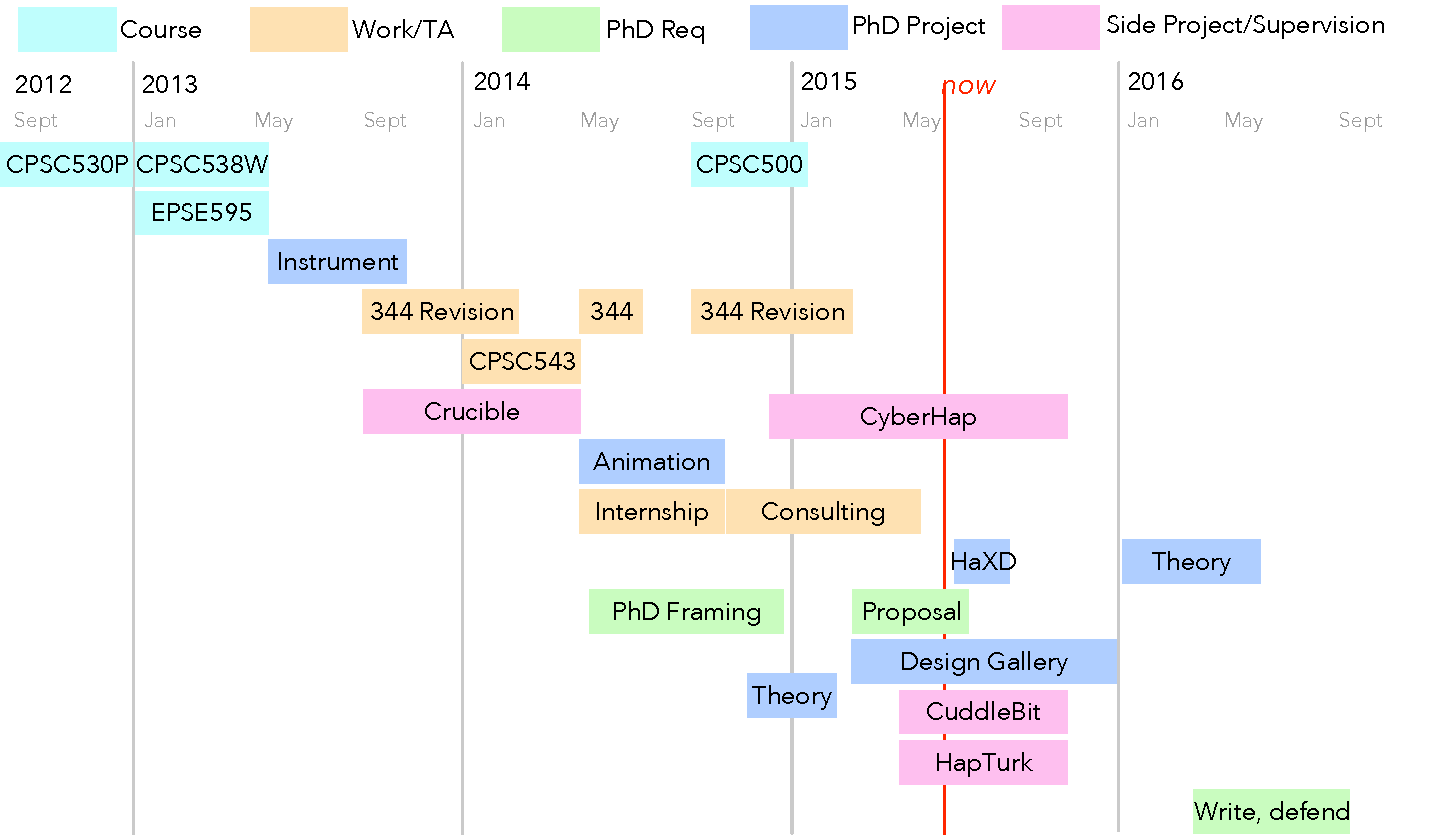
\includegraphics[width=\textwidth]{PhDTimelineOverview-2015-05-28} 
   \caption{Overview of PhD from start (September 2012) to intended finish (August 2016).}
   \label{fig:timeline:overview}
\end{figure}

\begin{figure}[htbp] %  figure placement: here, top, bottom, or page
   \centering
   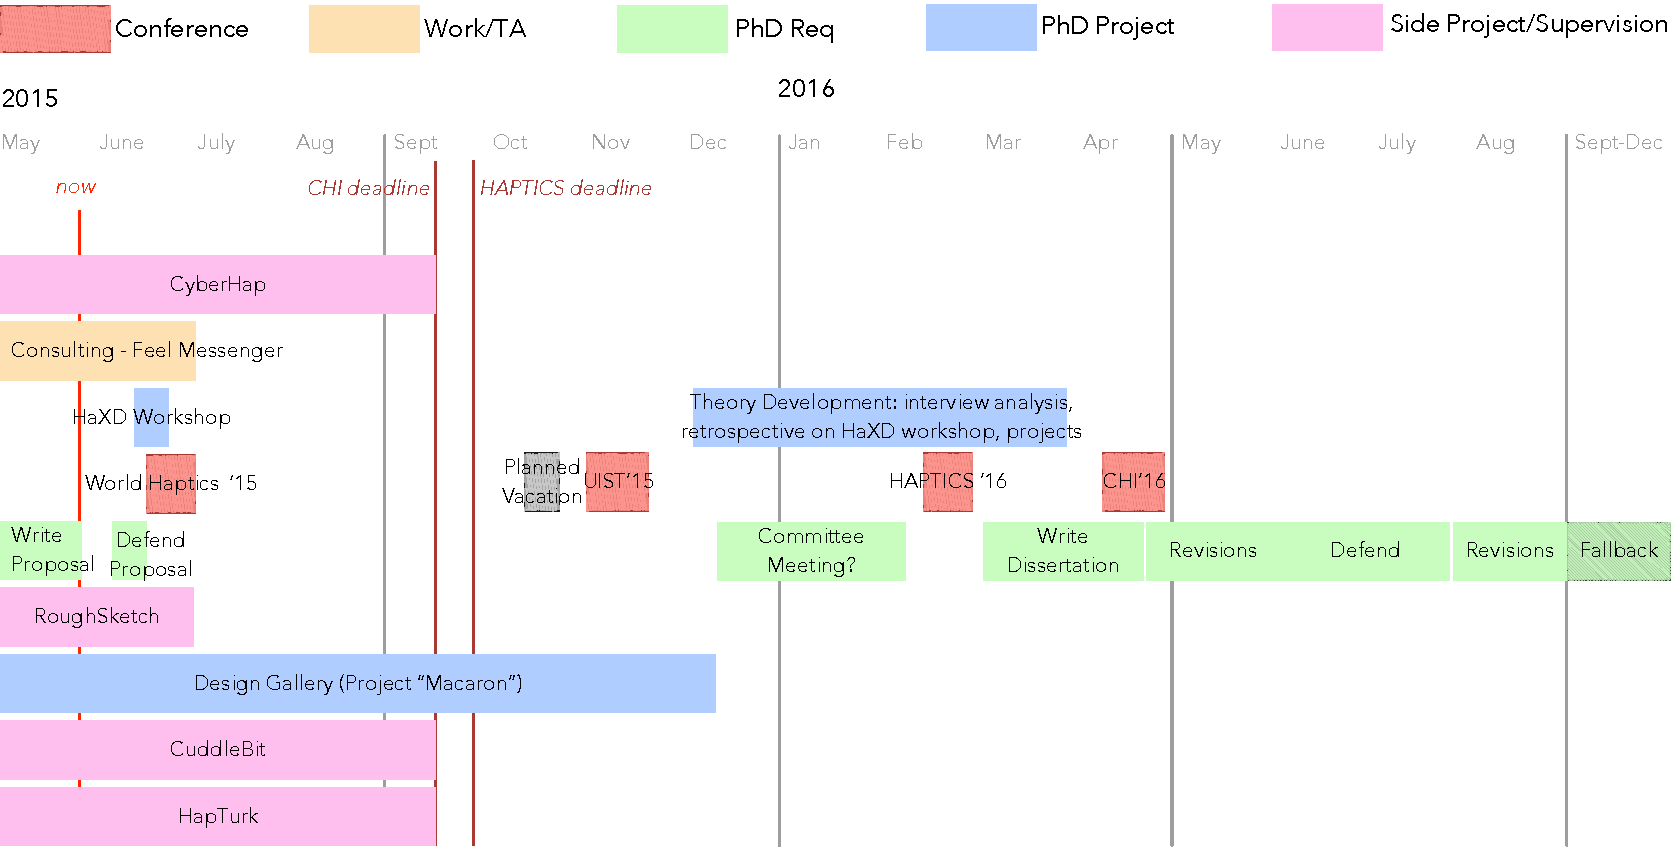
\includegraphics[width=\textwidth]{PhDTimelineZoom-2015-05-28} 
   \caption{Detailed timeline of remaining plans, from May 2015 to intended finish (August 2016). Note that several projects are targetting the CHI'16 deadline, but could also be submitted to the coinciding HAPTICS deadline based on fit.}
   \label{fig:timeline:zoom}
\end{figure}

\endinput


%%%%%%%%%%%%%%%%%%%%%%%%%%
%%%
%%% Chapter - Conclusion
%%%
%%%%%%%%%%%%%%%%%%%%%%%%%
\chapter{Conclusion}
\label{ch:conclusion}
In this dissertation, we explored haptic experience design (\haxd), looking at its process to inform how to design, build, and evaluate \haxd support tools.
%We leave the specific findings from each of our studies as best articulated in their respective chapters.
In this chapter, we summarize our research contributions from the preceding chapters and provide final thoughts about the \haxd process and support tools.
In particular, we discuss process, including challenges and strategies haptic designers can use to overcome those challenges, and
findings with specific implications for designing and developing software tools to support \haxd.
We conclude with directions for future work and final remarks on supporting \haxd.

\osE{Only so much can be done in the scope of a PhD dissertation, and so we note that this is not a complete description of \haxd.}
\osE{Our case study approach gave us a balance of depth, breadth, and grounded information; our selections for each information source necessarily shape our findings.}


%%%%%%%%%%%%%%%%%%
%
% Section - Description of the HaXD Process
%
%%%%%%%%%%%%%%%%%%
\section{Summary of Research Findings}
We summarize our more specific findings organized by approach: depth, breadth, and grounded capstone.


\begin{figure}[htbp]
\begin{center}
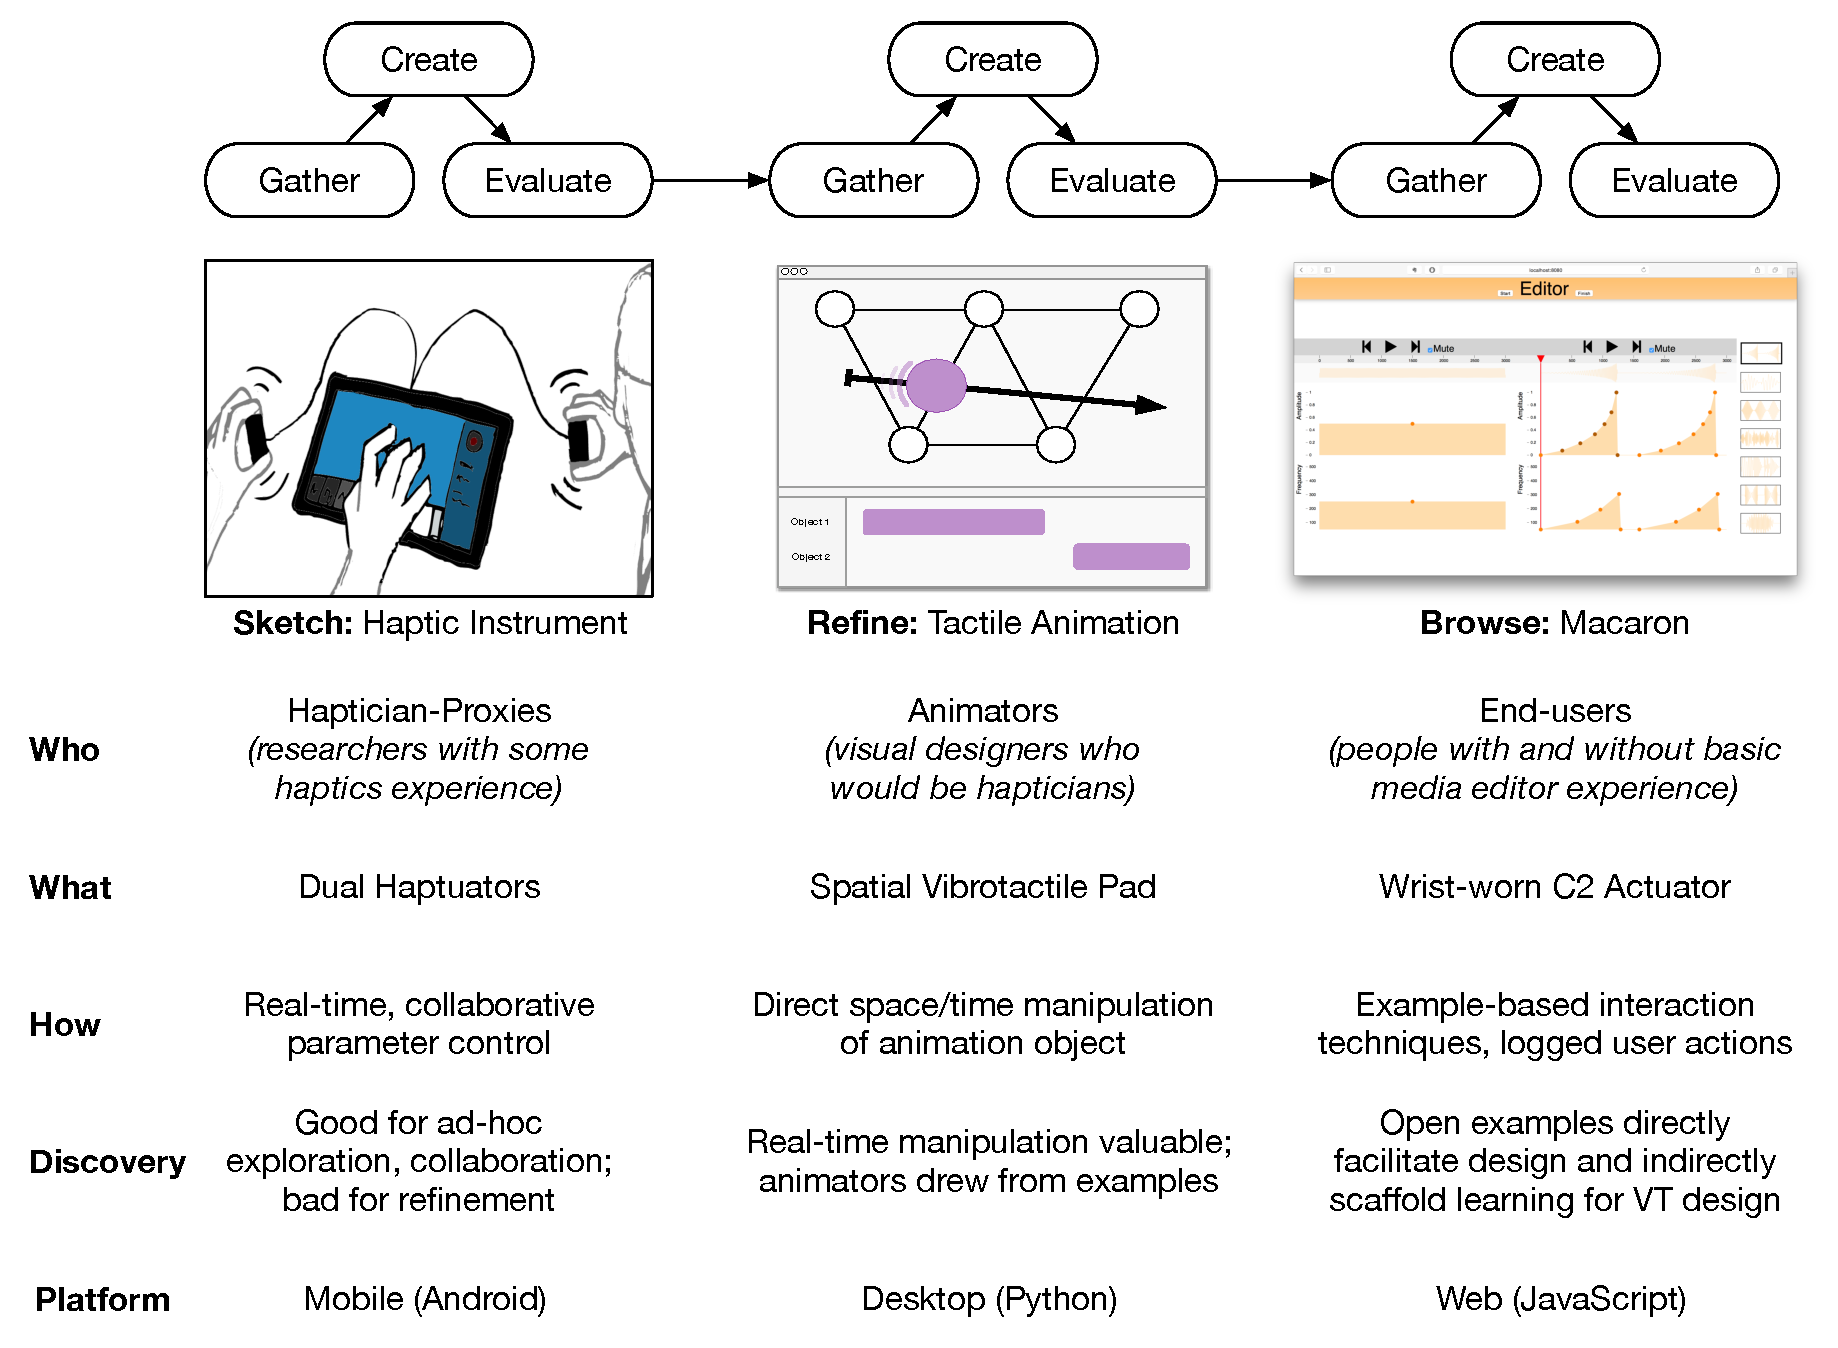
\includegraphics[width=\textwidth]{HaXDTheoryCaseStudyOutline-2016-12-22}
\caption{\revFinalKM{Vibrotactile} design case studies. Each studied an aspect of vibrotactile design with a varied set of users, devices, platforms, and foci.}
\label{fig:intro:casestudyoverview}
\end{center}
\end{figure}



\subsection{Depth: Vibrotactile Design Tool Case Studies}
Through Chapters \ref{ch:hapticinstrument}-\ref{ch:macaron} we designed, built, and studied a trio of \haxd support tools.
Each case study investigated a different set of design concepts with varying user populations, VT devices, and design challenges (\autoref{fig:intro:casestudyoverview}).
%Each followed three design steps: \emph{gather}, finding requirements and previous design elements; \emph{create}, where we design and build the tool; and \emph{evaluate}, where we test the tool with its target population and consolidate lessons learned.
We include HapTurk (\autoref{ch:hapturk}), a VT \emph{sharing} technique, in this discussion.
We began with an initial hypothesis: that real-time feedback and collaboration could improve the haptic design process.
Through our tools, this hypothesis was confirmed, elaborated, and refined.

\inlineHeading{Initial Exploration: The Haptic Instrument (\autoref{ch:hapticinstrument})}
In Study 1, the Haptic Instrument, we focus on real-time, rapid design of VT sensations with a first look into themes of real-time design and collaboration.
%When participants worked with our tool, mHIVE, compositions couldn't be edited, suggesting mHIVE was suitable for exploration and improvised communication, but not as suited to refining ideas.
%We also found informal, collocated collaboration useful, but leave future examination of collaboration support to side projects (described next in \autoref{ch:intro:approach:breadth}).
Our implemented haptic instrument, mHIVE, showed us that rapid exploration was possible with real-time feedback, demonstrated value in informal, collocated collaboration, and gave evidence that showing rather than telling about haptic sensations could circumvent an impoverished language (\eg, what do you think of \emph{that}).
 mHIVE also showed us that there are distinct roles to be played by different tools: mHIVE was successful for early \emph{sketching}, but did not enable \emph{refining}\revRG{.} %and had a learning curve.


\inlineHeading{Direct Manipulation Pipeline: Tactile Animation (\autoref{ch:tactileanimation})}
%In Study 2, Tactile Animation, we developed a single abstracted animation object directly manipulated in both space and time.
%In this study, we focused on building a usable tool to support exploration and refinement, and investigate a generalized rendering pipeline in detail to understand how to build haptic design tools.
%Animators found our tactile animation tool, Mango, easy-to-use, and confirmed our findings about the value of real-time exploration.
%We also found that ``soft features", like copy/paste and undo/redo, were extremely important.
Our second tool, Mango, followed up on these themes with a focus on implementation.
We established a rendering pipeline for both design and playback.
A direct-manipulation metaphor let participants both \emph{sketch} in real-time and \emph{refine} their designs.
In addition, an animation paradigm enabled our visual animators to transfer their skills to tactile animation.
Our evaluation study found evidence for reuse: repetition played a large role in tactile animations, and participants again drew inspiration from their experience or external examples (\eg, a YouTube video of a heartbeat) - and noted the engagement of multimodal design, \eg, designing for an audio clip.
These both informed Macaron.


\inlineHeading{Example Use and Analytics: Macaron (\autoref{ch:macaron})}
%One stand-out result from both Mango and mHIVE is that designers drew from their experience or examples found in the world, and wanted to re-use what they had created (e.g., through copy and paste).
%In Study 3, we explore the role of examples in haptic design with a web-based tool, ``Macaron", a vibrotactile track-based editor with visible, incorporable examples directly embedded in the interface.
%Macaron was implemented using the understanding we gained from Study 2, giving us more opportunity to focus on capturing and studying the design process, especially using interaction logs to investigate example use.
%%This study is codenamed ``Project Macaron" and consists of two phases.
%%Phase I, ``algorithms and interaction techniques", builds a set of perceptually-verified ways to manipulate examples and incorporate them into designs.
%%In Phase II, we use the results of Phase I to create a haptic design gallery interface, and study how and when users incorporate examples into their VT designs.
%%In this way we hope to consolidate our findings from mHIVE and Mango, and capture our participants' design process more concretely through logging of user actions.
%We found examples were used primarily as templates to inform initial design, making each individual design easier but also scaffolding the user's understanding of how to create VT effects.
%%These studies are described in more detail in \autoref{ch:hapticinstrument},  \autoref{ch:tactileanimation}, and \autoref{ch:macaron}.
With our third tool, Macaron, we were able to easily implement the system (drawing from Mango's architecture), allowing us to study our participants' process more closely.
We found a number of concrete recommendations for \haxd tools, and confirmed the value of \emph{browsing} examples: we found different strategies for using examples in the initial design process, and open or visualized examples helped designers learn how to conduct VT design.
 Macaron also helped us find our more nuanced understanding of our initial hypotheses. Real-time feedback is useful as a preview, to get the right frequency, amplitude, or timing. However, participants would also step back to feel the entire design in its entirety\revFinal{.}

\inlineHeading{Feedback at Scale: HapTurk (\autoref{ch:hapturk})}
	%is a collaboration with PhD candidate Hasti Seifi on different techniques to crowdsource feedback on VT icons. Master's student Salma Kashani and undergraduate Matthew Chun are developing visualizations and low-fidelity VT icons during summer 2015.
	While not an iterative design tool study, HapTurk is a focused investigation of a VT design technique for collecting large-scale feedback on VT icons.
%	Haptic devices cannot be sent to hundreds or thousands of people for feedback, but collecting in-lab feedback can be expensive, and informal feedback from colleagues is limited in scope.
%	We investigate whether visual or low-fidelity \emph{proxies} can stand in for high-fidelity VT effects, with implications for both collecting feedback and broadcasting VT sensations more widely.	
	HapTurk (\autoref{ch:hapturk}) allowed us to study \osE{a specific piece of collaboration: how to widely transmit designs.}
	% collaboration more thoroughly, as we focused on other aspects of design with Mango and Macaron.
	We found that VT icons could be \emph{shared} over MTurk to elicit large-scale feedback from remote users.
	We also found affective qualities of VT icons could be communicated through proxies, suggesting we can express haptic ideas in different modalities.


\subsection{Breadth: Focused Haptic Design Projects}
\label{ch:conclusion:approach:breadth}
Together, mHIVE, Mango, and Macaron have informed us on both important features and roles for design tools, given us insight into implementation and evaluation, and helped us study \haxd as a process.
HapTurk extended this investigation to collaboration.
%To further our understanding, we conducted several focused projects which broadened our understanding of different devices and application areas.
To broaden our understanding of haptic design, we undertook several focused haptic design projects to look at different activities, application areas, and haptic modalities.
In \textbf{\autoref{ch:applications}}, we described several smaller projects that gave opportunities for practicing haptic design and exploring other types of haptic feedback:

\inlineHeading{FeelCraft (\autoref{sec:applications:feelcraft})}  a plug-in architecture that augments media with customizable spatial VT effects.
	FeelCraft explored existing infrastructure for haptic media, and for designing VT effects for a popular video game, MineCraft.
	
\inlineHeading{Feel Messenger (\autoref{sec:applications:feelmessenger})} a chat program augmented with expressive, customizable VT effects using commodity hardware and APIs.
	
\inlineHeading{RoughSketch (\autoref{sec:applications:roughsketch})}  a painting application for the TPad Phone, a variable-friction mobile device, for the World Haptics 2015 Student Innovation Challenge. 
	Variable friction is a significant contrast to VT sensations as it is intrinsically connected to input: no sensation can be felt without active movement by the user.
	
\inlineHeading{HandsOn (\autoref{sec:applications:handson})} a conceptual model for creative education software using low-cost, DIY haptic hardware, giving us an understanding of how to work with 1-degree of freedom force feedback and an educational context.

\inlineHeading{CuddleBit (\autoref{sec:applications:cuddlebit})} a project inspired by the Haptic Creature \cite{Yohanan2011affectivetouch,Yohanan2011affectdisplay,Chang2010} and CuddleBot project \cite{Allen2015cuddlebot}.
	We use small, breathing robots to explore the display of emotion, and extend our findings from VT design tools into new tools for this modality: Voodle and MacaronBit.

\revFinal{These focused design projects implicitly enrich our final takeaways with additional insight gained from practicing \haxd, and explicitly contributed to our findings about device generalizability (\autoref{sec:generalizingdevices}) and metaphors for design (\autoref{ch:conclusion:framing}).
The CuddleBit tools also served to test our hypothesis about supporting \emph{sketching} and \emph{refining} with two separate tools.}



\subsection{Ground: Data from Hapticians}
In \textbf{\autoref{ch:hapticianinterviews}}, we complement our design-based inquiry with data from \revFinal{hapticians}, who are difficult to access as they are both rare and often work in proprietary contexts, with limited ability to speak about their process.
To include hapticians' perspectives without severely hindering our design tool development, we conducted a grounded theory analysis of interviews with six haptic designers.
We characterized cross-cutting themes at three levels of scope: 1) the holistic nature of haptic experiences; 2) the collaborative ecosystem of haptic designers and related stakeholders; and 3) the larger cultural context of haptics in the public consciousness.
We augmented these interview findings with those from a workshop \osE{we} organized at a major international haptics conference, World Haptics 2015, which let us connect with \revFinal{hapticians} more widely.

Our findings showed that \revFinal{hapticians} follow a general user-experience design process, but with added challenges because they work with haptics.
We articulated these challenges, \osE{gave} concrete recommendations on how to make progress on them, and finally gave a vision of \revFinal{\haxd} as it might be practiced in the near future.
These results overlap with our findings from our design-based inquiry: some conclusions are confirmed, with similar themes emerging both from expert hapticians and our design studies; others emerged from only one source.


%%%%%%%%%%%%%%%%%%
%
% Section - Process/Requirements
%
%%%%%%%%%%%%%%%%%%
\section{\haxd Process: Requirements for Tools}
In this section, we examine our findings about the \haxd process. %, including challenges and strategies that designers can follow.
In \autoref{ch:hapticianinterviews}, we saw that haptic designers follow a familiar design process.
However, we also saw that there are unique challenges that differentiate \haxd from other modalities of design, which are confirmed by our work on \haxd support tools and our focused design projects.

We begin by discussing four design activities that occur generally in design, but need to be explicitly supported \revFinal{for \haxd:} \emph{sketch}, \emph{refine}, \emph{browse}, \emph{share}.
Then, we comment on some approaches for handling the diverse devices and modalities employed by haptic technology.
After, we discuss some techniques to imbue haptic experiences with meaning and realism.
Finally, we talk about the importance of customization and how to support it.

%%%%%%%%%%%%%%%%%%
% SubSection - Description of the HaXD Process
%%%%%%%%%%%%%%%%%%
\subsection{Contextual Activities of Design: Sketch, Refine, Browse, Share}
In our first exploration of \haxd support tools, the Haptic Instrument (\autoref{ch:hapticinstrument}), we found evidence that mHIVE was able to support exploration and sketches of haptic ideas, but not refinement into final designs.
mHIVE was also able to support collaboration in certain ways.
In our followup studies, we explored these activities that draw upon a designer's context, eventually arriving at four that we found are valuable when thinking about tool design: browsing examples, sketching new ideas, refining existing ideas, and sharing ideas with others (\autoref{tab:designactivities}).
These activities can occur at any point in the design process, and we do not propose them as an exhaustive list; for example, ``framing" \cite{Schon1982,Warr2005} could be claimed as an activity for design which may overlap with activities like \emph{browsing} and \emph{sketching}.
We focus on their utility in motivating features and specific tools to aid haptic experience designers.




% Requires the booktabs if the memoir class is not being used
\begin{table}[htbp]
   \centering
   \small
   %\topcaption{Table captions are better up top} % requires the topcapt package
   \begin{tabular}{@{} ll @{}} % Column formatting, @{} suppresses leading/trailing space
          \emph{Activity} & \emph{Important Features to Support for \haxd}\\
      \toprule      
      Sketch
	& Abstractability and ambiguity\\
	& Rapid iteration \\
      \midrule      
      Refine
	& Mature design tools\\
	& Adaptable interfaces\\
            \midrule      
      Browse
	& Representations of single sensations\\
%	& Collection classification and organization\\
	& Overviews, search, and skimming\\
            \midrule      
      Share
	& Capturing ideas\\
	& Remotely or asynchronously share haptics\\
   \end{tabular}
   \caption{\osE{Four design activities that are supported in other fields of design, but need explicit support in \haxd.}}
   \label{tab:designactivities}
\end{table}


%
% SubSub - Sketch
%
\subsubsection{Sketch}
Sketching allows people to form abstracted, partial views of a problem or design, iterate very rapidly and explore concepts.
The generalized notion of sketching can support other activities: sketches are a notation that can be shared, and provide a vehicle for annotating and iterating on designs.
Here, we use \emph{sketch} in contrast with \emph{refine}, to refer to embodied exploration, concept generation, and initial design.

Early in our exploration, we found that our Haptic Instrument, mHIVE, excelled for exploring a design space but faltered for refining sensations.
A real-time direct manipulation model in Tactile Animation facilitated both.
In Macaron, we observed different levels of exploration and refinement, discovering a pattern of focused adjustment and repeated reflection \cite{Schon1982}, where the designers stepped back to feel their design in its entirety, and zoomed in to adjust parts in detail.
We find this is a repeated pattern, where participants iteratively zoom in and out to different levels.
The mixture of focus also depended on the stage of design - early on, exploration and execution take a more prominent role, while later refinement has smaller adjustments and more reflection.
We have found this distinction useful when developing suites of tools, most explicitly when supporting design of CuddleBit behaviours: 
Voodle is a free-form \emph{sketching} tool, which can hand off to MacaronBit for \emph{refinement}.
Future work remains to be done to establish whether there are discrete levels of focus, or if they lie along a continuum.
In general, we've found two main features important for supporting \revFinal{s}ketching: \textit{abstraction and ambiguity}, and \textit{rapid iteration}.



%This is mostly heavily used early in design, and plays a role in collaboration (discussed more in ``Share'' below).
%Of course, such a central technique is used as a key way of thinking about experience design~\cite{Buxton2007}; 
%some even consider sketching to be the primary language of design, equivalent to mathematics as a language for natural sciences~\cite{Cross2006}.
%


\inlineHeading{Abstractability and ambiguity}
	Haptics suffers from a dearth of notation.
	Sketching of physical devices or interfaces is well supported, with paper and pencil and innumerable software assists.
	Sketching \textit{motion}, and in particular showing what is or might be felt in, say, a vibrotactile experience, is  trickier.
	While we can sketch a visual interface and look at it, it is much harder to sketch a haptic sensation and imagine it without feeling it.
%Most directly, \citet{Moussette2011} teach Haptic Sketching with physical scraps and materials, combined with manual actuator and tools like Arduino, to build effective interactive haptic prototypes physically and programmatically  in minutes or hours.
%Simple display-only sensations can be sketched (\eg, VT icons)  using interactive design tools \cite{schneider2014improvising,Hong2013}.
%\osC{What about a planning/execution/reflection pattern?}

\inlineHeading{Rapid Iteration}
Design requires fluid, playful interaction with potential designs and the associated problem space.
Haptic design sometimes requires fuzzy goals like feeling ``just right", requir\osE{ing} designers and users to feel \osE{design candidates}.
When iteration is slow, it is painful and distracting.


%
% SubSub - Refine
%
\subsubsection{Refine}
Design requires iteration to \emph{refine} an initial set of ideas into a single well-developed one through concept generation followed by iterative revision, problem-solving and  evaluation, until only small tweaks are necessary.
%This long view of the design process is necessary to see designs through to the end\osE{.}
\osE{Haptic experiences must leverage refinement to be tailored to each application area and support individual differences.}

Incorporating haptic technology into a design is an extremely vertical process,  dependent on  specifics of hardware, firmware, software, application, and multimodal context.
With the complexity of these many components, there can be a significant initial cost to setup a first haptic experience; then, adding this complexity to the time needed to program, recompile, or download to a microcontroller means iteration cycles have the potential to be slow and painful. 
There are two stand-out features to support refinement: mature, polished tools, and adaptable interfaces.
%
% Of course, there has been progress, and more is on the way. 
%Thus, increasing refinement fluidity is ripe for innovation. For example:

\inlineHeading{Mature design tools}
Implemented design tools require a glut of features, \eg, picture the sheer number of commands, shortcuts, and organizational scaffolding supplied by image editing software like Photoshop.
This power and precision can improve refinement, especially when integrated into haptic media pipelines to fluidly move initial ideas to final experiences. 
We describe the road to mature tools in \autoref{sec:conclusion:maturetoolsuite}.

%\inlineHeading{Evaluation} is as crucial as for any human-centered refinement cycle. While it will often require some form of \textit{sharing} (coming up next), here we simply point out that the full spectrum of evaluative mechanisms and supports found in user experience development can be gainfully applied to haptic design, from lab-based comparative performance studies to qualitative examination of how usage strategies change when a physical dimension is deployed (\eg, \cite{minaker:2016:EH:handson}).

%\inlineHeading{Customization tools} are appearing at least at level of prototyping and requirements generation \cite{SchneiderAsiaHaptics2014,Seifi2014}. 
%Force-feedback virtual environments support iteration and refinement through code, once the initial environment is setup.
%Software platforms like Unity\footnote{https://unity3d.com/} offer immediate control of variables in the UI itself.

\inlineHeading{Adaptable interfaces} 
Calibration, customization, and sensing were identified in \autoref{ch:hapticianinterviews} as one major approach for handling the varied end-user context. 
These techniques will be essential to ensure consistency and quality of refined sensations, or to let designers and users alike fine-tune their experiences.
We describe these in more detail in \autoref{sec:generalizingdevices}.
%in tools will help final haptic designs remain consistent depending on user activity (\eg, running impairs vibration sensitivity), individual differences, or other contextual concerns.


%
% SubSub - Browse
%
\subsubsection{Browse} 
``Browse" can have specific meanings for interacting with data \cite{munzner2014visualization}.
Here, we use \emph{browse} to refer more generally to the act of looking at examples, \eg, corkboards of previous designs \cite{Buxton2007}; drawing from previous personal and professional experiences, \eg, one's repertoire \cite{Schon1982}; or real-life sources to inform a design.
We found this emerged in different ways:
in \autoref{ch:hapticinstrument}, participants used their personal experiences to interpret sensation meaning (\ie, schemas, discussed more later);
in \autoref{ch:tactileanimation}, one animator brought up a YouTube video of a heartbeat to ground his animation;
in \autoref{ch:hapticianinterviews} several participants described collecting examples or using guide books.

We highlight this activity because haptic designers encounter modality-specific barriers when gathering, managing, and searching for examples.
Explicitly supporting browsing can make a difference:
in \autoref{ch:macaron}, we found visible, incorporable examples both eased design and helped scaffold learning for non-experts.
We believe scaffolding to be extremely important, as there are few haptic designers practicing today.
Browsing is also tightly associated with the ability to \emph{share} designs and collaborate; when one designer shares their designs or ideas, others are able to browse it.
We highlight \osE{two} main challenges to supporting browsing in \haxd: representation and access.
%meanwhile, industrial designer Raymond Loewy espouses the need to balance the familiar and the new in design, creating the ``most advanced yet acceptable" design [].



%No idea is born in isolation.
%Individual designers have a repertoire of previous experiences they've encountered while learning or through practice~\cite{Schon1982}.
%In addition, design often starts with a ``gather" step~\cite{Warr2005}: viewing examples for inspiration and problem definition.
%Gathering often occurs explicitly at the start of a design process, and can reoccur during iteration.
%Tangible examples are corkboards and mood boards, which allow ideas to ``bake in" to the background~\cite{Buxton2007}.
%Software tools like d.tour~\cite{Ritchie2011} and Bricolage~\cite{Kumar2011} recommend websites for inspiration and can automatically generate new ideas by combining sites.
%\osC{make sure this doesn't overlap too much with Background}


 \inlineHeading{Representations of single sensations:} 
    How do we store, view, and organize haptic experiences?
    Haptic technologies are often inherently interactive, part of a multimodal experience with visual and audio feedback, and can take a variety of physical forms depending on the output (and input) device.
%    This last point is particularly bothersome should the user not have access to the original device type -- imagine trying to browse force-feedback sensations on your phone!

%\inlineHeading{Collection classification and organization:}
%    Haptic language and cultures of meaning are still in active development.
%    Without a commonly shared lexicon, organization dimensions, or even adjectives, it is difficult to curate collections.
%    Compare this to sound: most musical terms have a long tradition with a clearly defined lexicon (\eg, crescendo, staccato); non-musical sound effects generally ``sound like'' something, and are often literal.
%    With vision, one does not have to be a graphic designer or artist to instinctively understand ``warm" and ``cool" colours; the color wheel is introduced to us in grade school.  
    
   \inlineHeading{Overviews, search, and skimming:} 
    Collections of examples, especially visual or physical collections, are often displayed spatially for ambient reference or to enable quick scanning.
    When you cannot feel multiple things, it can be hard to get the big picture or swiftly peruse a collection.
    Both designer and end-users have needs for finding similar or different vibrations in a collection. %, requiring a low barrier-to-entry on any overview technique.


%
% SubSub - Share
%
\subsubsection{Share} 
Sharing designs is valuable at different stages of the design process \cite{Kulkarni2014}, whether for informal feedback from friends and colleagues, formal evaluation when refining designs, or distributing to the target audience for use and community for re-use \cite{Shneiderman2007}.
As haptic experiences must be felt, this process works best when collocated with only a few collaborators, whether by having collaborators work in the same lab, or by showing final experience in physical demos.
During ideation, ideas can be generated when collaborating remotely, but physical devices need to be shipped back and forth and it is difficult to troubleshoot and confirm that configuration and physical setup are the exact same.
Feedback also typically needs to be collocated, using in-lab studies or feedback, or shipping devices between collaborators.
Furthermore, visual and audio design support very easy capture of ideas to share later, through smartphone cameras and microphones, that could later be browsed.
We suggest two  directions for future work: easy capture of design ideas to share for later, and remote sharing through proxies.

\inlineHeading{Capturing ideas}
Inspiration can strike at any time.
In order to \emph{browse} ideas later, or to snap a haptic picture and \emph{share}, we need advanced haptic cameras \cite{MacLean1996}.
Repositories are only useful when they are populated; easy capturing methods can encourage crowds to upload their own content for later use, perhaps leading to stock haptic experiences (like stock images) and a viable venue for freelance haptic designers.

\inlineHeading{Remotely or asynchronously share haptics}
Touch is a proximal sense, and difficult to share asycnhronously or over large distances.
Techniques like proxy sensations (\autoref{ch:hapturk}), easy calibration (\autoref{sec:generalizingdevices}), and fabricated haptics using, \eg, 3D printers \cite{torres2015hapticprint} can all help \emph{share} these physical sensations around the world.


%%%%%%%%%%%%%%%%%%
% SubSection - Paradigms and Representations
%%%%%%%%%%%%%%%%%%
\subsection{Generalizing Devices and Sensations}
\label{sec:generalizingdevices}
One major challenge facing haptic designers is the variety of haptic devices available.
Each device has different physical properties, and may use different actuation principles or sensory modalities to communicate with the user.
This might be analogous to how modern web sites employ responsive design, adapting to different screen sizes, albeit more extreme.
A screen, at the end of the day, is that plane with a given physical size and pixel size; with haptics,
contextual problems like grip can influence feedback, and haptic feedback can vary from single VT actuators to VT grids, programmable friction, skin stretch, or force-feedback devices.
We suggest three ways of managing this complexity:
\revFinal{g}rouping devices and interactions into \emph{paradigms},
considering representational \emph{translations}, and
using affordances and closed-loop sensing to create \emph{consistency}.
A fourth related strategy, enabling customization, is so important we discuss it later.

\inlineHeading{Paradigms}
First captured in Chapter \ref{ch:hapticianinterviews}, we believe that paradigms \osE{are} a key concept to designing \haxd tools.
We define a ``paradigm" as an abstracted model of how to work with a haptic device.
\osE{D}ifferent programming language paradigms, such as functional or object-oriented languages, enable programmers to think in different ways more appropriate to their problem\osE{.}
\osE{W}e believe that different haptic or multimodal paradigms will enable different problem solving techniques for \haxd.
In our in-depth studies we present three: an instrument paradigm, an animation paradigm, and a track-based editing paradigm.

There is a many-to-many mapping between paradigms and haptic devices.
Tactile animation can be used for multiple spatial grids and track based editors are generalized enough to handle multiple display types.
Meanwhile, a multi-VT grid could be controlled by any of these three paradigms.
As haptic displays become more diverse, we expect paradigms to play a larger role for organizing design perspectives, and multi-paradigm tools to become successful, just as multi-paradigm programming languages like Python and JavaScript afford flexibility, power, and accessibility - providing increasingly low barriers, wide walls, and high ceilings.


%\inlineHeading{Representation and Native Platform}
%One striking problem with haptic technology is its sheer diversity.
%There are a wide diversity of devices, many of which support different paradigms, and all of which can be different based on their physical configuration.
%This poses a problem of access - if a designer creates a force-feedback sensation, how do you render that on a mobile device with a simple vibrotactile actuator?
%Can this translation be done?
%
%Compare this to graphic design.
%At the end of the day, most graphic designs will be on a 2D plane, whether a screen or not.
%There are different sizes, resolutions, and colour maps - for example, print media might be designed differently than web - but similar tools and principles apply.
%In haptics, we might apply these different sizes and resolutions to a class of device - for example, a VT actuator can be an expensive C2 tactor or a low-cost voice coil.
%However, a single actuator is quite different from a 2D grid of actuators (like in Tactile Animation), and dramatically different from variable friction feedback (like with Rough Sketch) or 1-DoF force feedback (like with HandsOn).
%The question of resolution and platform within a single class of devices is analogous to the challenges faced by graphic designers and sound designers, but the diversity of classes of devices is even more varied.

\inlineHeading{\osE{Consistency through Adaptable Interfaces}}
%\inlineHeading{Consistency through sensors and context control}
%\subsubsection{Adaptable Interfaces}
%\label{sec:conclusion:adaptableinterfaces}
%We've shown how individual differences are a prominent feature of haptic perception and psychology.
\osE{V}ariability in and poor designer control over context --  user attention and  device form factor and manner of connection, as well as use environment -- mean that haptic sensations often need to be tuned to both each person and each use case.
In \autoref{ch:hapticianinterviews}, we suggested that adaptable interfaces could help manage changing context and encourage consistency and appropriate feedback.
%A third way to adapt to the variety of contexts a haptic device might be used in is to either impose a known context, or sense and adapt an uncontrollable context.

Our industry haptic designers would talk about working with automotive companies, and how the material in the dashboard could affect the final haptic sensation.
By controlling this material and working in a known environment, haptic designers might be able to keep their designs more consistent\osE{.}
%When actuating a touch-screen in a car, a designer could know the materials.
Similarly, wearable devices like the wristbands (Pebble, Apple Watch) have a known location on the user; designers can use that knowledge to their advantage. They can also use the materials of their wrist-straps to ensure a reliable tightness or pressure on the skin.
Force-feedback devices like haptic knobs might change their handles, using physical affordances to suggest a grip to the user.

Alternatively, closed-loop sensing might be able to standardize sensations.
\citet{Blum2015} showed that accelerometers can provide insight into perceived loudness of VT stimuli.
Techniques like activity classification (\eg, \cite{Schneider2013}), or even vibration sensing of a VT effect could help reduce noise from physical changes and material properties.
This could be done \emph{in-situ}, or during manufacturing for different device materials as a quality assurance step.

\osE{E}nd-users might benefit from \textit{customiz\osE{ing}} aspects of haptic design elements, whether by choosing pre-formed settings and ``skins'', adapting defaults, or wholly designing their own. 
Possible approaches range from volume-like slider controls, options to select sensations from curated collections, or, at the more complex end, perceptually-confirmed filters like those found in Instagram or PhotoShop~\cite{Seifi2014,Seifi2015,SchneiderAsiaHaptics2014}.


%%%%%%%%%%%%%%%%%%
%
% Section - Meaning
%
%%%%%%%%%%%%%%%%%%
\subsection{Framing and Meaning}
\label{ch:conclusion:framing}
\revFinal{In our focused design projects (\autoref{ch:applications}), we found that having a cohesive, intentional conceptual framing was critical for compelling haptic experiences.}
We suggest three ways of designing meaning into haptic experiences:
schemas and metaphors,
design languages,
and reinforcement through narrative context and other modalities.



\inlineHeading{Schemas and Metaphors}
Schemas are existing conceptual models used as transitional objects to \revRG{understand} new concepts \cite{Papert1980}.
We found this procedure occurred not only in educational contexts, but also in design.
In our early Haptic Instrument exploration, we found our participants' prior experience was a lens through which they interpreted haptic sensations.
For example, one cat-owning participant interpreted sensations as cat purring, while another drew on their knowledge of engines and cars.
Heartbeats and rain \cite{Israr2014} are effects that were easily understand by general participants, and verified using perceptual studies.
Schemas are useful both for framing user interpretation of haptic experiences, and for designers themselves.
\osE{M}any previous systems have their roots in other, non-haptic concepts, \eg Touch TV \cite{Modhrain2001}.
This enables transfer effects; visual animators were able to easily create tactile designs \osE{using} Tactile Animation (\autoref{ch:tactileanimation}).

%\osC{KM: This part was mostly written by Hasti. However, browse emerged partially }
%To interpret haptic signals, people employ a number of conceptual or translational  schemas, often combining them.  % frameworks
%We might compare a haptic sensation to a natural one (``This is like a cat purring''), 
% to emotions and feelings (``This is boring'''), or
%consider its potential usage (when a quickening tactile pulse sequence is described as a ``speed up''). 
%%
%The meaning someone chooses is typically influenced by the sensation itself but also by the context of use and the user's background and past experiences~\cite{Seifi2015, schneider2014improvising, Obrist2013}. 
%
%%\begin{figure}[bt]
%%        \centering
%%        \includegraphics[height=2.5in]{figures/InterpretiveFacets3}
%%        \caption{People use a variety of cognitive frameworks to make sense of haptic signals.}
%%        \label{fig:interpSchemas}
%%    \end{figure}
%    
%\textit{Facets} are a concept originating from the domain of library and information retrieval which nicely capture the multiplicity and flexibility of users' sense-making schemas for haptic sensations. A facet is a set of related properties or labels that describe an aspect of an object~\cite{facetedbrowsing2010}. Five descriptive facets have been proposed and examined for haptic vibrotactile stimuli \cite{Seifi2015}: physical properties, sensory properties, emotional connotations, metaphors, and usage examples.
% 
%%    \textit{\textbf{Physical}} properties that can be measured -- such as duration, energy
%%    
%%    \textit{\textbf{Sensory}} properties -- roughness, softness
%%    
%%    \textit{\textbf{Emotional}} connotations -- pleasantness, urgency 
%%        
%%    \textit{\textbf{Metaphors}} or familiar examples to describe a vibration's feel -- drumbeat, cat purring
%%    
%%    \textit{\textbf{Usage examples}} or types of events where a vibration fits -- ``speed up'', ``time's up''
%
%If a designer neglects a consistent consideration of these meaning assignment facets % frameworks, 
%the result is likely to be confusion and bad user experience.
%Leveraged properly, facet-driven 
%mappings can be lead to more intuitive, consistent results and highlight pathways to work around individual differences, for example through tools that allow users to efficiently customize their interfaces.
%
%Schemas can also be used for haptic designers to help frame their design processes.
%As covered in \autoref{ch:rw}, many previous systems have their roots in other, non-haptic concepts, \eg Touch TV \cite{}.
%This enables transfer effects; as we showed with Tactile Animation (\autoref{ch:tactileanimation}), visual animators were able to easily create tactile designs.

\inlineHeading{Design Languages}
Another way of framing a haptic experience is to use a \emph{design language} like Google's Material Design (\url{https://material.google.com}).
A design language is a defined set of aesthetic and interactive rules to ensure a consistent look-and-feel.
\revFinal{Hapticians can structure a haptic experience (or platform for haptic experiences) by developing rules about how and when to use feedback, and what each type of feedback means to the user.}
\revFinal{A haptic design language %We also believe that Gestalt-like principles will play a role in defining the possible design languages for haptics,
could be structured in different ways, for example, using} %much like
musical concepts of thematic development, restatement, elaboration, and expectation, or graphical design concepts like contrast, repetition, alignment, and proximity\revFinal{.} % are the tool with which languages can be formed.
Previous efforts have identified frequency, amplitude, rhythm, affect, and spatial location as the main design elements for vibrotactile design.
We have started to identify similar, middle level concepts - alignment and repetition emerged in the Macaron study.


\inlineHeading{Narrative Context and Multimodal Reinforcement}
The intent of a haptic sensation \osE{is} not always interpretable from the sensation itself.
A great deal of the interpretation of an effect depended on the narrative context.
Previous work used linguistic descriptions, such as ``light rain" \cite{Israr2014}.
In our FeelCraft and Feel Messenger studies, we found that linking adaptable sensations to in-game stimuli was effective.
With Feel Messenger, we at first attempted feel effects with abstract icons, such as ``motor" for a rumble effect. 
In early piloting, these were not very helpful for understanding.
Adding in vibrant cartoon emoji icons, and using  a cat's face (for a purr) rather than a motor image were much more effective in sending haptic icons.

%It is also worth mentioning the role of realism in a haptic experience.
%There are two types of realism, photo-realism (veridicality) and real-seeming (verisimillitude) \cite{mccloud1993understanding}.
%For example, cartoons are clearly not depictions of reality (they do not display veridicality), but they can appear life-like (they display verisimilitude).
%In this dissertation, we focused on verisimillitude rather than veridicality; the latter is often already accommodated by realistic rendering techniques.
%We believe both require a design process, but more photo-realistic approaches have different challenges than cartoony ones, and may require more of an engineering perspective than a design perspective.
%That said, sometimes combining the two is helpful\osE{:} in computer graphics, physical simulation and realistic rendering are \osE{augmented} by artistic control over certain scenes or effects.
%






%\inlineHeading{Volume Controls}
%As found in our interviews with designers, the end-user context is sometimes unknowable.
%There is not much designers can do other than putting a volume control on their design to facillitate customization.
%In informal discussions with engineers from commercial companies (\eg D-Box), volume controls were a critical, early addition to their haptic chairs.
%As explored in our FeelCraft and FeelChat projects, the extra level of volume control is implementable, expressive, reduces footprints, but is more limiting for designers and requires programming expertise.
%While there is a great deal of noise in perceptual parameters for high-level controls, careful investigation can improve this \cite{Israr2014,Seifi2014}.
%
%
%
%\inlineHeading{Novelty and Irritation}
%Haptic sensations are new, giving them great power and great responsibility.
%They can grab attention, but designers must take care not to annoy with constant haptic feedback.
%The balance is tricky. 
%Good design might be not even noticed when present.
%With RoughSketch, we found that allowing a button to remove haptic feedback was very persuasive for appropriate, non-irritating designs.
%We also found that muting features were essential for \haxd design tools.






\section{\haxd Tools: Designing and Implementing}
In this section, we comment on the specific features and forms \haxd support tools might involve.
Because of the diverse activities described in the previous section, we believe there is no silver bullet: haptic design tools are likely to form a suite or ecosystem.
Here, we discuss ways to enable creativity through mature tools with ``a low barrier, wide walls, and a high ceiling."
We \revFinal{first} talk about important collaborative techniques and how to deploy implemented tools.
We \revFinal{then} discuss implications for developers and software engineering teams.
Finally, we conclude with some comments on our evaluation methodology and how future \haxd tools might be evaluated.


%%%%%%%%%%%%%%%%%%
% SubSection - Online Communities
%%%%%%%%%%%%%%%%%%
\subsection{Communities and Online Deployment}
\revFinal{H}aptic technology faces obstacles to \emph{browsing} and \emph{sharing}, especially when under development\revFinal{.} 
\revFinal{Prototypes are typically shown with in-person demos, which} 
are difficult to setup. % and there is little infrastructure in place for distribution.
While \revFinal{demos support} synchronous, collocated collaboration, remote or asynchronous collaboration is rife with trouble.
Consistency must be maintained, and setup can be painful for those not trained in setting up devices.
\revFinal{In addition, an impoverished language for talking about touch hinders communication,} especially for non-experts.
%Without a shared reference point of physically feeling the sensation, we believe that design can be easier, especially when a language of design is underdeveloped.

\revFinal{To improve support for browsing and sharing, we suggest improving online infrastructure to distribute content and knowledge for both hapticians and end-users}. 
%We found that \revFinal{building a} web-based tool (Macaron) greatly facilitated distribution.
Online deployment widens exposure and speeds development, making it easier for designers to be inspired by or directly build upon one another's work. 
\revFinal{We comment upon two ways online infrastructure can help designers: through crowdsourcing and broadcasting, and by building sharing communities.} %xpect more online resources to be developed} as the field matures, but there will need to be concurrent development of accessible hardware to connect with software tools.

\inlineHeading{Crowdsourcing and broadcasting} 
    We reviewed some of the substantial challenges and spoke of one type of solution.
    In HapTurk (\autoref{ch:hapturk}), we showed proxies of high quality haptic experiences  can communicate key aspects on more shareable media, to gain access to crowdsource evaluation tools like Mechanical Turk.
    Proxies might be able to generalize in other ways, for example, using video to infer feedback about physically moving objects like the CuddleBits. % (\eg, as in \cite{Pedersen2014}).

    Proxies can do more than elicit feedback from crowds.
    It might also be a viable way to translate sensations between representations, analogous to downsampling high-definition video broadcasts for standard definition televisions.
    More exotic proxies, like using vibrotactile feedback to represent force or friction, could be considered. 
    Future perceptual studies are needed to accomplish this.
    
\inlineHeading{Open Haptics -- design sharing communities} 
    % While remote engagement can introduce other issues, they not only provide corresponding benefits but also can be complementary to existing practices. 
    Other kinds of designer-facing online communities and outreach activities may assist with open haptic media -- making it easier to share design resources \revFinal{and} build up a haptics design culture. %, and, where possible, cooperate on establishing a consistent design language of haptics. 
%
    For example, online software like VibViz~\cite{Seifi2015} and Macaron~(\autoref{ch:macaron}) provide details to \revFinal{hapticians} anywhere, while open hardware projects like HapKit~\cite{Martinez2016} and Haply~\cite{Gallacher2016} are available to hackers and students.
    Conference workshops and hardware kits provide users and designers with additional means to experiment with advanced haptics.
    
    Each of these projects solve different problems and provide independent benefits.
    Online collaboration, and resources like articles on haptic perception or tutorials on how to effectively create haptics, will connect more designers, artists, developers, students, and hackers and help to build haptics into new user experiences.


%\inlineHeading{Show, don't tell}
%We found that demonstrations were critical for haptic designers in the wild.
%To help elicit requirements, customers were brought in to try out various demos.
%To persuade customers, actually feeling the haptics was critical, if not always enough.
%The Haptic Instrument showed evidence for deictic features \osE{(\eg, ``}what do you think of \emph{this}\osE{?")}, which facillitated direct demonstration without having to resort to indirect linguistic descriptions.
%In Macaron, exposing the underlying structure of examples led to improved understanding of how to develop sensations and developed haptic idioms.


%%%%%%%%%%%%%%%%%%
%
% Section - Towards Mature Tool Suite
%
%%%%%%%%%%%%%%%%%%
\subsection{Towards a Mature \haxd Tool Suite}
\label{sec:conclusion:maturetoolsuite}
\osE{Given the diverse activities that need to be supported for \haxd, we envision a suite of tools to support haptic designers.}
\osE{Here, we outline important features that we believe will enable such a suite}

%%%%%%%%%%%%%%%%%%
% SubSection - Examples
%%%%%%%%%%%%%%%%%%

\inlineHeading{Soft Features}
Repeatedly, participants asked for ``soft features", associated with more polished tools.
This includes features like copy and paste, undo and redo, saving and loading, grouping, looping, reduced delay, and high-fidelity rendering.
We increasingly found, as we iteratively developed \haxd tools, that these features are more important than getting the right paradigm.
As long as a \revFinal{haptician} is able to freely and accurately create, she can work around awkward design metaphors.

%\inlineHeading{Low barrier, wide walls, high ceiling}
%A major goal of our work was to support creativity with haptic technology, and to support low barriers, wide walls, and a high ceiling \cite{Shneiderman2007,Resnick2008}.
%We've confirmed that this is critical for \haxd, and found ways of accomplishing it.
%As we mentioned, our participants found soft features essential, which helped to free them to make mistakes \revFinal{and} explore various options\revFinal{.} %, and provide both accessibility (low barriers) and refinement (high ceilings).
%For example, in Tactile Animation, participants found the animation objects easier for exploration and non-expert designers, while vector sensations offered more fine-tuned control.
%Similarly, we found the more flexible track-based paradigm used by Macaron to allow for various paths through the interface, and was generalizable to other sensations like simple 1-DOF robots.


%
%Making haptics means different things at different stages in the process. 
%Media creation in other modalities is supported with a wealth of tool specializations that recognize these diverse needs. Haptic making has reached a maturity that demands tool power, nuance, and specialization as well.
%
%Some of the important ground to cover here includes better support for \textit{sketching}, \textit{high-level manipulations}, \textit{multimodal qualitative analysis} and \textit{browsing}, as well as workflow integration and addition of specific useful features to tools that already do exist.

%
% SubSub - Sketching
%
%\subsubsection{Allowing Sketchiness}
%Early design needs support for low-cost, rapid ideation that elevates key points without extraneous detail. Haptic design presents a few challenges; solving these will further empower designers.
%
%\textit{Ambiguous sketches} show only necessary detail or relevant view points, helping a designer work with half-formed ideas and questions, but a haptic sensation requires a physical implementation which must be exactly specified. 
%%
%We need to explore different approaches to quick prototyping of different haptic aspects -- \eg, feel, form factor, timing. One approach is \textit{modularity}: prototyping one aspect at a time, then integrating into more expensive engineering prototypes once the design space has been narrowed. Here, the tool need is both for ready-to-go platforms to explore single-aspect ideas, and ways to efficiently extract, port, or integrate best-of-breed sketches into later design stages.
%    
%\inlineHeading{Good defaults:} In another approach, designers will be able to select from carefully chosen default settings, and/or specify  any known constraints with other details be filled in automatically. 
%    
%\inlineHeading{Annotation:} Sketching should supply markup support for both early-stage designers themselves and the stakeholders they share with, to  annotate sketches, circle problem areas, and write down related ideas.
%    
%\inlineHeading{Ad-hoc use:} Finally, tools should be easy to access. With a pen, any napkin is a canvas. Haptics (and multimodal interactions in general) need napkins too. 
%
%
%%
%% SubSub - Low-level
%%
%\subsubsection{Fluid control of low-level parameters}
%A viable approach enabled by our real-time tools is an implicit understanding of the sensations by designers, who were able to work with low-level engineering parameters like frequency, amplitude, or even voltage.
%In the Tactile Animation study, we found that while animation objects were more used and described are more accessible for non-animators, vector sensations (directly controlling each actuator) were described as useful for finer, expert control.
%Learning to control low-level parameters is important for ``high ceilings" in \haxd support tools.
%
%
%
%%
%% SubSub - High-level
%%
%\subsubsection{High-Level Manipulations} 
%The haptics community currently has access to a number of editing tools which together exhibit a variety of approaches to editing and authoring, primarily of low level effect detail (Section~\ref{sec:make_tools}).
%However, being able to manipulate sensations in the large or in an expressive way will enable designers to access a larger design space, and do more in less time.
%
%In other modalities (Photoshop for graphic media, Audacity for sound), this kind of functionality appears in a variety of ways.  
%\textit{Filters} are essentially ``tuners'' that move a sensation along dimensions of direct design interest.
%\textit{Transformations} allow users to alter or distort a segment, \eg, to darken or brighten it,  stretch its time base in a linear or nonlinear way, or shift component balance.
%%
%\textit{Large-scale manipulations} can move, combine, subtract and otherwise alter design elements.
%
%The scope of such manipulations should span perceptual, informational, and affective perspectives. Research is underway to understanding these manipulations from user perceptual and subjective standpoints, and implement them algorithmically. 


%
% SubSub - Engineering features into mature tools
%
\inlineHeading{Engineering useful features into mature tools} 
\osE{There is value in} seamless access to many small but useful features\osE{, like}
direct manipulation, undo \osE{and} redo, copy \osE{and} paste, selection and group manipulation, \osE{and} import \osE{and} export to various formats.
%
Individually, many of these do not present major research or usability problems, but integrating them is another matter.
There are at least two obvious approaches: additive and haptics-specific.

    Haptics authoring capability can be added to existing mature platforms focused on another modality -- \eg, to Photoshop (for graphics)  or Premier (video).
    Force-feedback is already integrable into certain video game and virtual world environments (\eg, Unity, XNA), but this is only a subset of possible haptic experiences.

    To truly optimize haptics capabilities, it may be worthwhile to invest serious development into a haptics-specific platform; or more likely, many attempts at such a thing focused on different categories of hardware (\eg, tactile wearables versus 3D desktop force feedback environments) or application area, perhaps by extending initial low-level editors already available.

%Researchers are good at pioneering individual steps and features, but integration is a significant development initiative which lies more in the province of businesses who stand to profit by the effort invested. 
%Which task focus and development pipelines are to be supported, including multimodal design and integration,  will be driven by application areas with urgent needs and a promising economic prognosis:  \eg, for movie special effects versus surgical simulations or end-user customizations.


%%
%% SubSub - Engineering features into mature tools
%%
%\subsubsection{Iteration}
%In our interviews, we found iteration was extremely painful.
%Despite this, we've found iteration is necessary (as with all design processes), but even more so because it is difficult to understand requirements or identify a good design without feeling it.
%Many of our designers would iterate until it ``felt right".
%Thus, iteration is very necessary yet very painful.




%%%%%%%%%%%%%%%%%%
%
% Section - Implementation
%
%%%%%%%%%%%%%%%%%%
\subsection{Notes on Implementing \haxd Tools}
During our in-depth studies, we looked at three different platforms for implementing \haxd support tools: Android on tablet for mHIVE, Python on desktop for Mango, and JavaScript deployed on the web for Macaron.
From these three implementations, and from attempting to distribute or deploy them, we have found several lessons for implementing interactive software for \haxd support.
%Many of these are straightforward applications of software engineering, but we particularly found recently developed web tools to be especially useful when managing the complex interfaces required by design tools.

\inlineHeading{Observer Pattern}
Well established as a software engineering design pattern, we found the observer pattern was critical in keeping the complex interfaces of our design tools synchronized.
This is especially critical because we need to synchronize haptic, audio, and video playback, and allow implementations through both temporal and spatial means.
In Mango, we implemented this pattern ourselves, but in Macaron, we used React to automate this process.
%This latter approach was more efficient and facillitated programming.

\inlineHeading{Components and Track-based Editing}
Another valuable approach to develop extensible tools was React's \osE{c}omponents, interface elements that can be parameterized and reused.
This technique, along with a carefully organized architecture and the generic track-based editor control paradigm it very easy \osE{to extend Macaron}.
W\osE{e were able to build the first version of MacaronBit}  in a single day.
%While a \osE{more appropriate} paradigm could be designed, our in-lab experts were able to used generalized tracks to create differentiable behaviours from the bit.
%One can also imagine redesigning a track-based editor to use a different control paradigm with the same device - we do this with MacaronMix, which mixes two VT icons using again a fork off of Macaron.


\inlineHeading{Flexible, extensible data structures}
Because of the complexity and variance of haptic devices, we \osE{employed lightweight, extensible data structures:}
\osE{Mango, Macaron, and FeelCraft} used JavaScript Object Notation (JSON).
JSON allowed us to specify only the required information needed, whether for device parameters in Mango, or sensations created by both Mango and Macaron.
Our tools would check JSON files for designed features - like amplitude tracks in Mango - and \osE{accommodated stubs for unsupported features} - like frequency tracks.
These structures were simple, human-readable, ignored extraneous detail, and could gracefully fail when poorly formatted\revFinal{, and thus support the diverse, rapidly changing set of available haptic devices.}
%Because we need to accommodate different paradigms in \haxd tools, lightweight data types make a lot of sense.

\inlineHeading{No Delay}
In interviews with designers, we found that delay was critical; multimodal sensations had to be tightly synchronized.
We found similar problems with our tools.
mHIVE had a short delay which was distracting to participants, particularly when they tried to play very short pulses\osE{;}
Macaron's real-time audio synthesizer sometimes created a ``muddy" effect because it had a limited update rate.
We found this disappeared after we implemented a .WAV exporting function.
Combined with our findings that users would switch between focused, in-depth editing and more reflective experiencing, we suggest (and are working to implement) a pre-feel/render model, like with visual effects tools.
%This is one potential problem with current web implementations of our design tools, especially when attempting to communicate to embodied devices like Arduino.

\inlineHeading{Distribution requires hardware}
An obvious, but critical, requirement for \haxd tools is that they require the appropriate hardware.
Above we've discussed flexible architectures and data structures to support different hardwares and paradigms of sensations.
In addition, potential \revFinal{hapticians} need easy access to hardware\osE{, \eg, through self-assembled DIY devices, online distribution methods, or translating to existing platforms like phone vibrations.}
%One way we've found is to create do-it-yourself haptic wristbands for Macaron. 
%Critical for VT feedback is that amplifiers and actuators matter - we found the DIY custom amplifier we've built does not have the same crispness as a more expensive commercial audio amplifier.
%This means that modular systems could be designed for facillitate accessible haptic feedback and design, but are complicated in because the setup doesn't end at the actuator.
%Another approach is to use a HapTurk-based translation with mobile vibrations like those available on Android (link to hapticJS), although this impoverishes sensations and leads to the challenge of native platform, discussed above.


\inlineHeading{Logging and Analytics}
One important feature for modern software is remote analytics.
Various types of metrics and usage statistics help developers prioritize development, fix bugs, and report to investors.
\osE{B}ecause haptic technology extends into the physical world, one can consider using remote analytics both on software and on physical devices.



%%%%%%%%%%%%%%%%%%
%
% Section - Evaluation
%
%%%%%%%%%%%%%%%%%%
\subsection{Evaluating \haxd Tools}
\osE{Creativity-support tools do not yet have standardized evaluation methods \cite{Shneiderman2007}.}
\osE{During our in-depth studies, we iteratively developed methods from previously established methodologies and techniques.}


%%%%%%%%%%%%%%%%%%
% SubSection - Flow, learning, scaffolding
%%%%%%%%%%%%%%%%%%
%\subsubsection{Flow, Learning, Scaffolding, and Embodiment}


%\subsubsection{Exploratory Analysis and Visualization Tools (Haptic Analytics)} 
%Haptic researchers frequently analyze haptic datasets with the goal of informing next steps in a design use case or deriving design guidelines for the haptic community. 
%Such an  investigation usually involves exploratory analysis of quantitative and qualitative attributes of signals and users' perceptions. 
%Currently, designers use a potpourri of general-purpose software (\eg, Matlab, R, SPSS, Tableau) for their analysis. Each tool provides just a partial view of the data; the difficutly of integrating their insights hinders the analysis process. 
%
%Visual analytics interfaces, which support analytical reasoning through interactive visualization of datasets, are largely absent from haptics at this time. 
%Examples of desirable functionalities  include easy access to the feel and source of signals, enabling rapid and flexible organization of haptic signals according to their various properties, allowing researchers (and the crowd) to attach metadata (tags, genealogy, annotations) to elements and subsets of a haptic collection, and do analytics on this metadata.
%
%
%The first steps towards haptic analytic interfaces (Section~\ref{sec:make_tools}) have exposed some of the work that's needed to make these truly useful. Much of it is the same underlying perceptual knowledge and  algorithmic advances required for authoring and manipulation, \eg, of perceptual dimensions and user's mental organization and ways of differentiating and interpreting sensations, and this is well underway. 
%%
%Connection to or integration of multimodal functionality -- \eg, suitability for coordinating with design elements from other modalities, in various communication roles (Section~\ref{sec:IM_roles}) -- will develop along with our experience in working with these modalities. 



\osE{Post interviews were effective.}
Early in our investigation, we found that participants found traditional think-aloud protocols challenging.
\osE{Attention was already split between perceiving} sensory input on their hand while simultaneously designing sensations.
%Even without thinking-aloud, this was cognitively challenging, and participants wanted looping, or would step back to refine and feel their sensations.
In response, we adopted unintrusive logging and post-interviews, both of which were effective in capturing aspects of the haptic design process. 

\osE{Phenomenology and grounded theory methods worked well together.}
Because of the close connection with participant experience, we adopted techniques from phenomenology, both to capture the sensory experience of haptic sensations, and \osE{the} experience of design.
This perspective was useful for rigorous examination of our participants' interviews and to guide the interview process.
In addition, the practical techniques \osE{like} clustering \osE{statements} into both in-vivo language and analytical language \osE{were a concrete way to manage interview analysis.} % very useful, especially when later combined with Grounded Theory techniques.
To better equip ourselves to analyze larger sets of data and develop a broader theory, we also drew upon grounded theory as described by Corbin and Strauss \cite{Corbin2008}.
Especially when analyzing screen-captured video, coding techniques \osE{helped} identify countable data and add\osE{ed} a second layer of data analysis to complement phenomenology.

\osE{Later quantitive analysis complemented qualitative results.}
Qualitative analysis of post-interviews provided valuable insight, but only gave a partial view of \osE{\haxd}.
Timing analysis and visualized logs captured data that may not have been observed by the researcher \osE{or} reported by the participant in a post-interview.
\osE{Analytics} also offer a transition into \osE{scaling} data collection \osE{for deployed tools.}
\osE{However, some quantitative scales were most useful because of the discussions they inspired.}
\osE{Rating scales of} confidence and difficulty \osE{were not trustworthy with the small sample sizes used in our in-depth studies.}
%We did not find \osE{these ratings to be trustworthy quantitative metrics.} %from these reports, mostly due to low sample size and the qualitative nature of analysis.
%However, we did find \osE{them} useful for two reasons.
\osE{These ratings provided} an elicitation device, inviting participants to \osE{verbally} comment on the difficulty of or their happiness with their designs.
\osE{A}s we scale to more natural settings and higher sample sizes, we hope quantitative findings from rating scales will provide \osE{additional} insight. % to questions about challenge, learning, and \osE{creativity}.


\osE{Design tasks needed to be carefully chosen.}
With the initial Haptic Instrument study, we asked participants to freely explore the interface and attempt to design for affective words like happy or sad.
This was challenging for participants. %, and we found inconsistent designs. \osC{TODO: what exactly was bad about this?}
In our Tactile Animation study, we used more defined scenarios - a heartbeat, a directional cue for driving, and a sound-based design task.
The first two were effective and descriptive for our participants, but the sound task in particular engaged them; it also gave us controls over theoretical dimensions like complexity or abstractness \osE{and} was externally valid with the multimodal nature of haptic design.
In our final in-depth study, we adopted animations instead of sounds, with similar results.





%%%%%%%%%%%%%%%%%%
%
% Section - Future Work
%
%%%%%%%%%%%%%%%%%%
\section{Future Work}
The next steps for this work are to directly follow up on our synthesized recommendations to establish \haxd, continue to expand our our tools and evaluation methods, and invert the premise of this thesis: use haptic technology to support design and problem solving.

We are already following up on our synthesized recommendations.
Macaron was deployed online, along with a preliminary DIY haptic wristband and amplifier\footnote{\url{http://www.instructables.com/id/MacaronKit-USB-Powered-Mono-Audio-Amplifier}} to enable anyone, anywhere to start prototyping vibrotactile icons.
We are planning to develop 3D printed models and online distribution methods to further facilitate artists, designers, and makers to work with haptic technology.
We are also reaching out to other haptic researchers to find a way to connect their work with end-users through tutorials, articles, and other online tools.

Next, we plan to expand our tools to support more paradigms, haptic sensations, and evaluation methods, primarily using Macaron as a development platform.
We are actively developing MacaronMix, an extension of Macaron which support interpolation of VT icons using novel algorithms; this new tool paradigm takes two \emph{browsed} examples and directly combines them.
We also seek to expand Macaron's output modalities to include directional capabilities, such as that explored by tactile animation, and to further develop the user logs from \autoref{ch:macaron} into an analytical suite to further capture the haptic design process.
More generally, we plan to follow up on our findings on Csikszentmihalyi's theory of flow \cite{Csikszentmihalyi1996} as a means to evaluate creativity-support tools.

\revFinal{Another area for future work is to evaluate the final designs produced by our tools.
In this dissertation, we looked at user process and self-rated approval of produced designs.
Future work can have end-user ratings of designs to determine if certain tools or techniques influence, \eg, diversity or quality of final output of designs \cite{Kulkarni2014}; we are already looking at the user-rated affective range of CuddleBit behaviours produced with Voodle and MacaronBit.}

Finally, haptic technology can support design, problem-solving, and sense-making.
Learning benefits from physically embodied interactions \cite{Papert1980}; meanwhile, professionals like architects, designers, and psychiatrists approach each new problem or patient with fresh eyes, seeking to learn about it \cite{Schon1982}.
We believe that the link between haptic technology and creativity runs both ways.
Possibilities include developing accessible sense-making platforms \cite{Swaminathan2016}, and exploring creative, haptic therapy to promote mental wellness.

%%%%%%%%%%%%%%%%%%
%
% Section - Conclusion
%
%%%%%%%%%%%%%%%%%%
\section{In Closing}
Our technology continues to push us toward a mixed reality, where physical objects compute, and people can enter realistic virtual worlds.
We strive towards computers that speak on human terms, both in end-user experiences by engaging all of our senses, and by supporting human creativity when designing those experiences.
\osE{Haptic technology is poised to reach out and connect with our senses of touch.}
\osE{By understanding haptic experience design, and how to support it, we can encourage and enable the advantages offered by this emerging modality.}



\endinput





%    3. Notes
%    4. Footnotes

%    5. Bibliography
\begin{singlespace}
\raggedright
\bibliographystyle{abbrvnat}
\bibliography{refs/HA14-CHI2015-SIGGRAPH-add,refs/HA14-CHI2015,refs/HapticDesignChallenges-WHC2015,refs/HI-HS2014-refs,refs/verillo2,refs/proposal-bib}
\end{singlespace}

\appendix
%    6. Appendices (including copies of all required UBC Research
%       Ethics Board's Certificates of Approval)
%\include{reb-coa}	% pdfpages is useful here
%%
% Appendix: Supporting Materials
%

\chapter{Supporting Materials}
\label{ch:SupportingMaterials}


\section{Study Forms}
\label{ch:SupportingMaterials:ConsentForms}

	%Main consent forms
	\subsection{Primary Study Forms}
	\label{ch:SupportingMaterials:ConsentForms:Primary}
	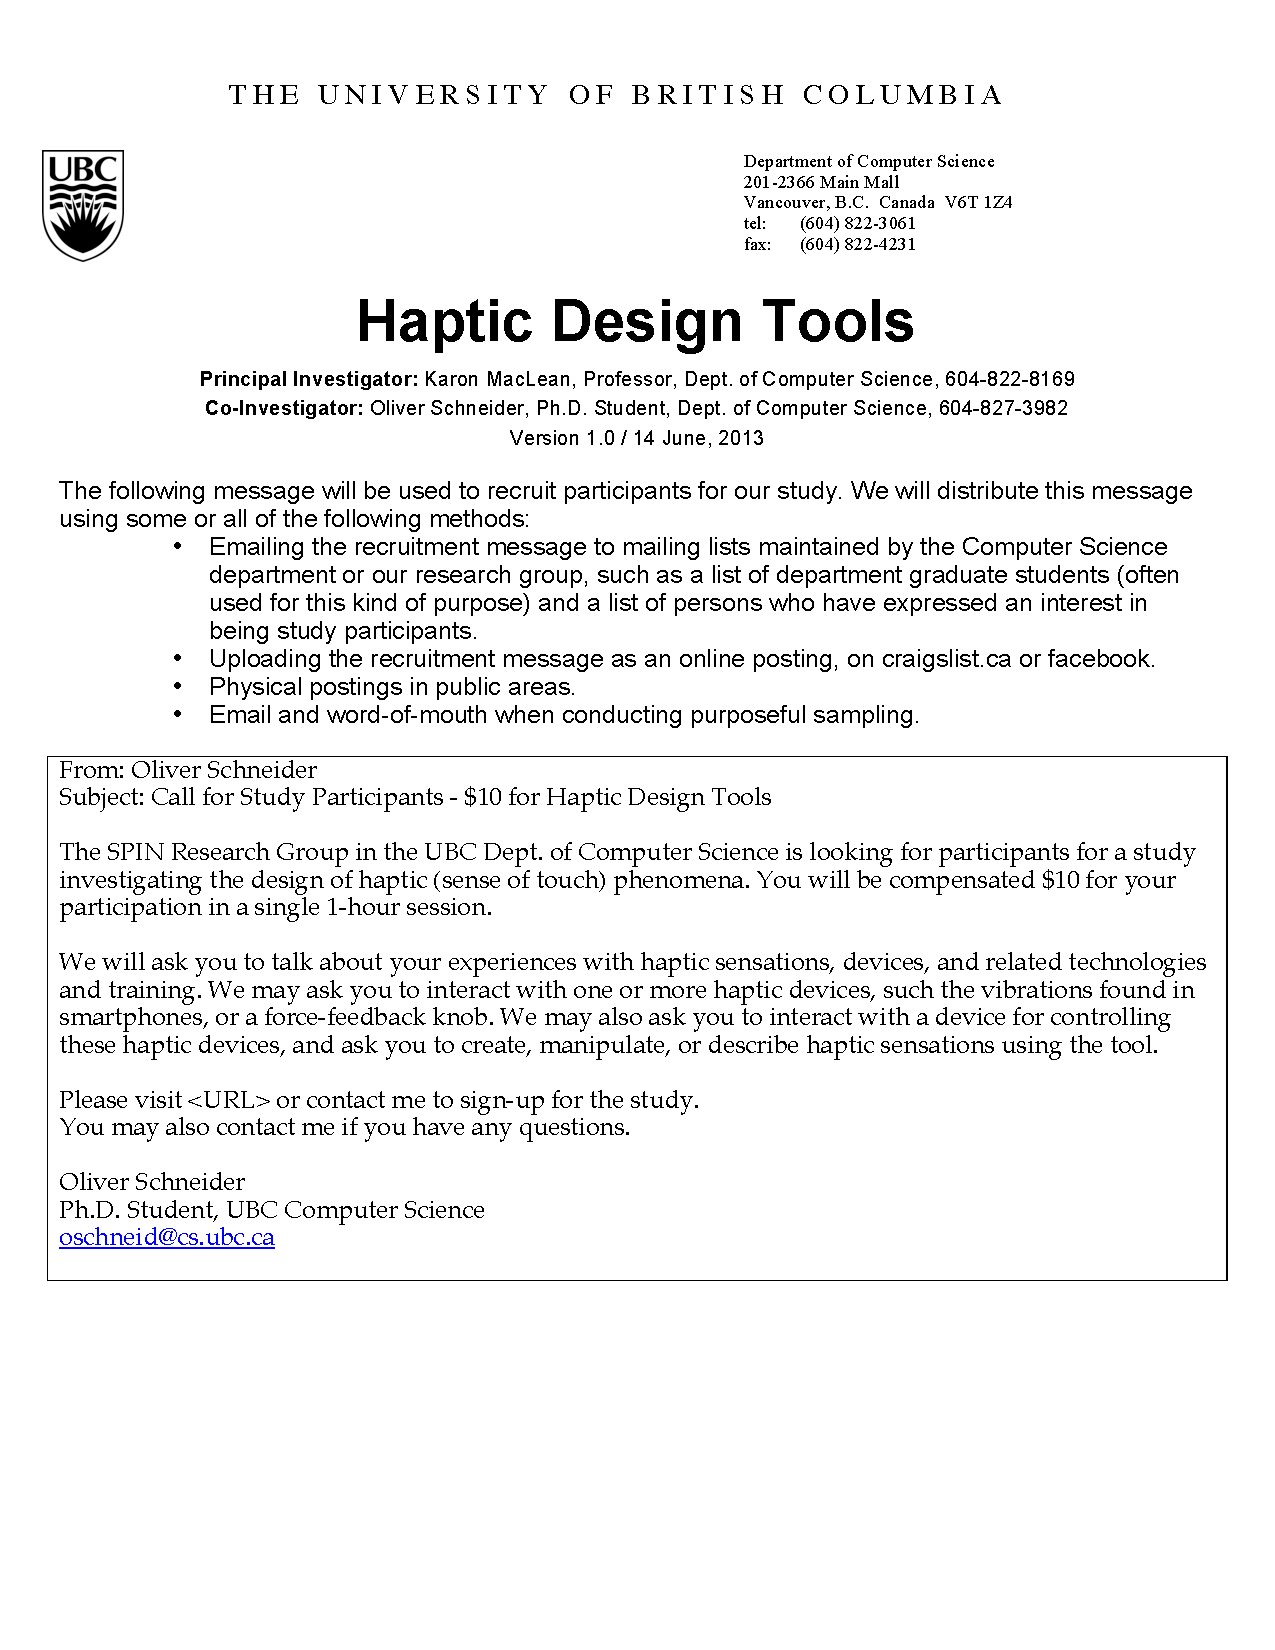
\includepdf[pages=-, pagecommand=\thispagestyle{plain}, width=1.25\textwidth]{Chapter99-SupportingMaterials/MainEthics/HapticDesignTools-CallForParticipation-v01-2013-06-14}
	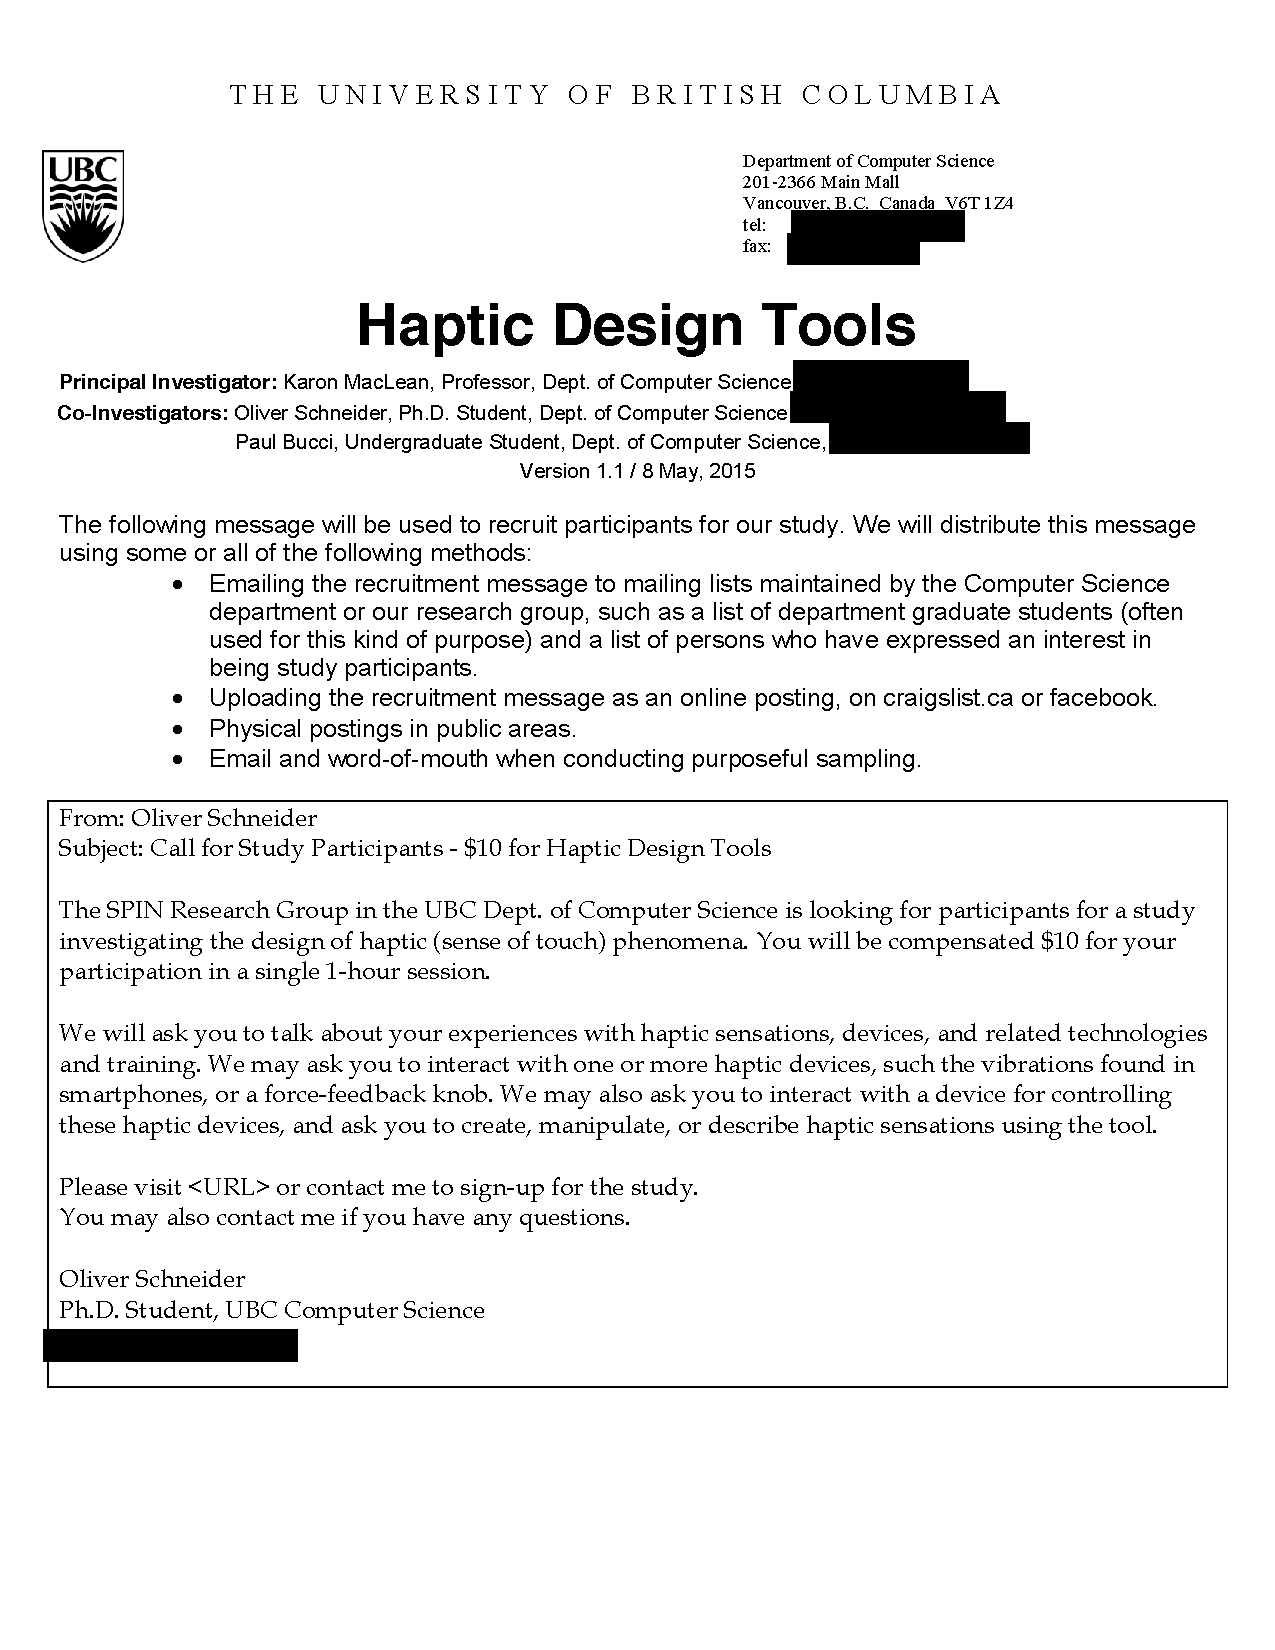
\includepdf[pages=-, pagecommand=\thispagestyle{plain}, width=1.25\textwidth]{Chapter99-SupportingMaterials/MainEthics/HapticDesignTools-CallForParticipation-v11-2015-05-08}
	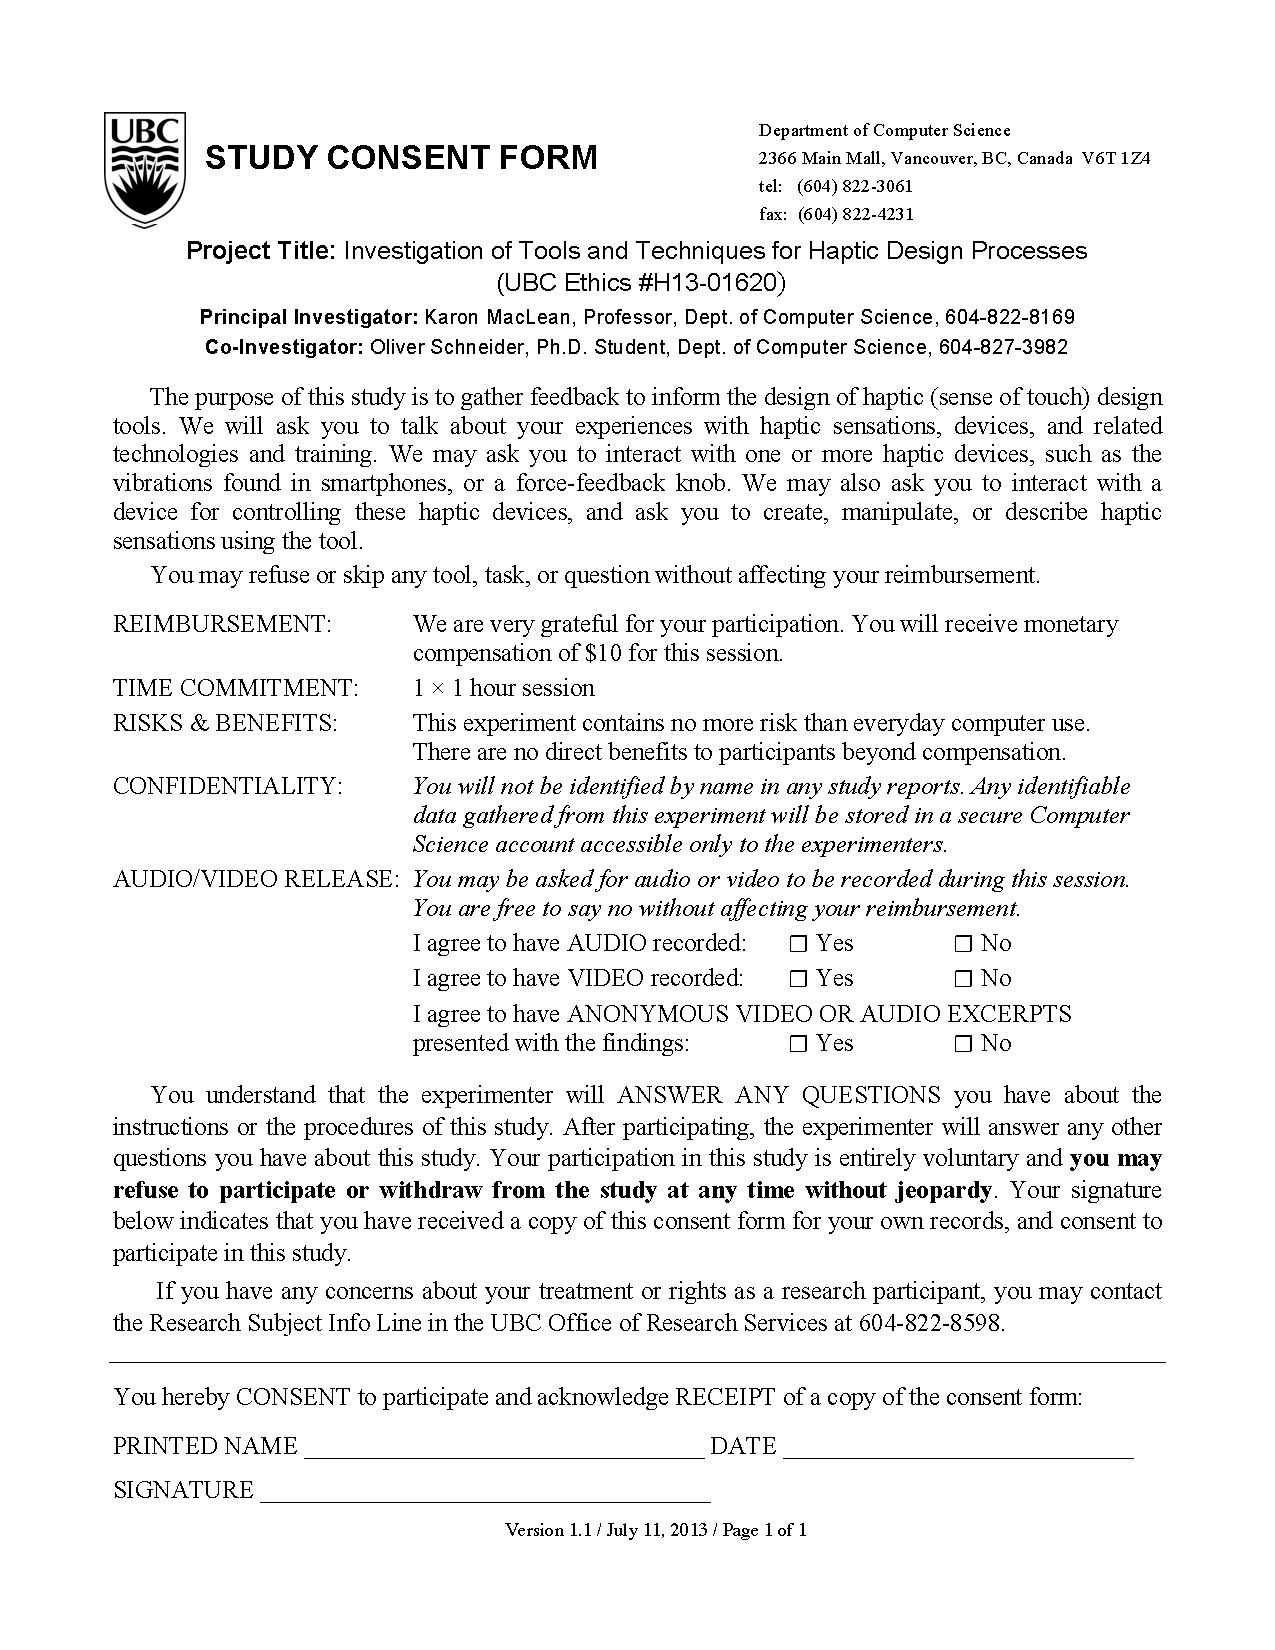
\includepdf[pages=-, pagecommand=\thispagestyle{plain}, width=1.25\textwidth]{Chapter99-SupportingMaterials/MainEthics/HapticDesignTools-Consent-v11-2013-07-11}
	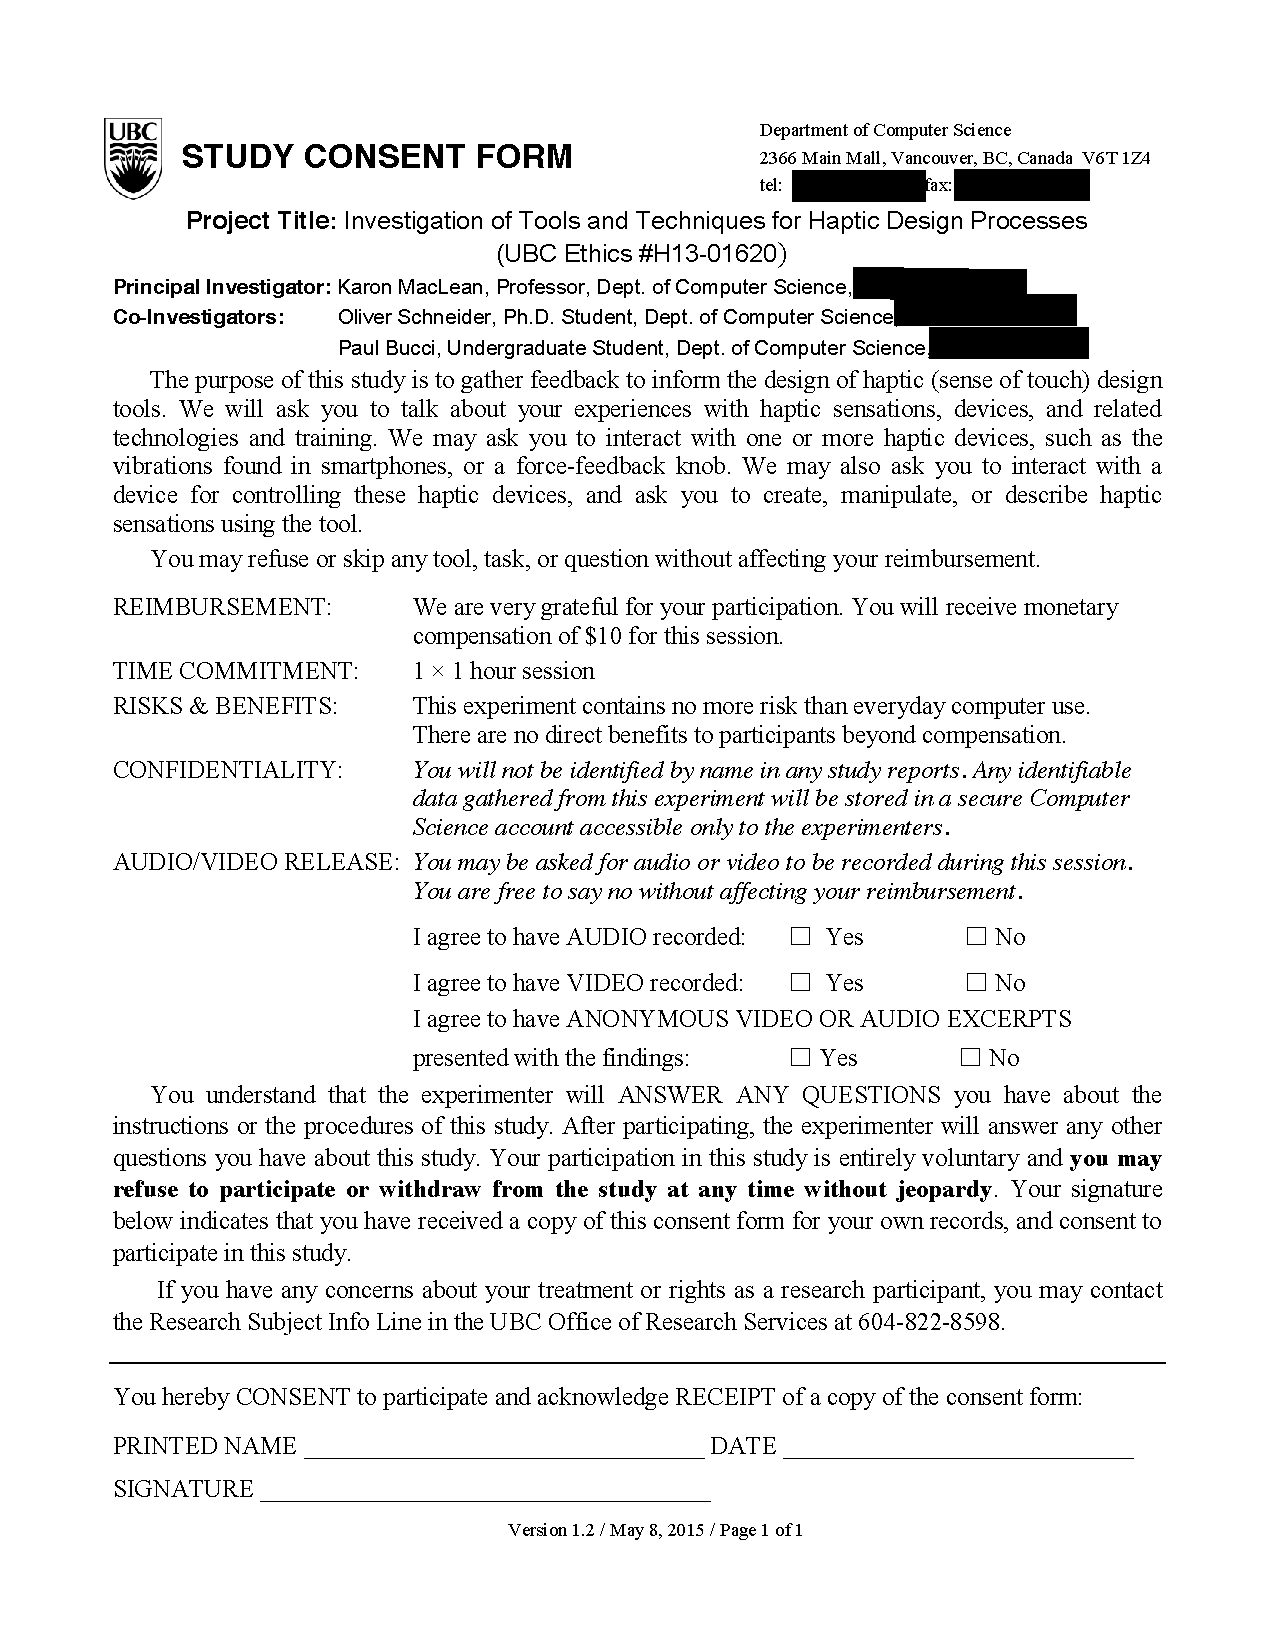
\includepdf[pages=-, pagecommand=\thispagestyle{plain}, width=1.25\textwidth]{Chapter99-SupportingMaterials/MainEthics/HapticDesignTools-Consent-v12-2015-05-08}
	\includepdf[pages=-, pagecommand=\thispagestyle{plain}, width=1.25\textwidth]{Chapter99-SupportingMaterials/MainEthics/HapticDesignTools-RequestForFollowup-v01-2013-6-27}
	\includepdf[pages=-, pagecommand=\thispagestyle{plain}, width=1.25\textwidth]{Chapter99-SupportingMaterials/MainEthics/HapticDesignTools-RequestForFollowup-v11-2015-5-8}



	%tactile animation
	\subsection{Tactile Animation Forms}
	\label{ch:SupportingMaterials:ConsentForms:TactileAnimation}
	\includepdf[pages=-, pagecommand=\thispagestyle{plain}, width=1.25\textwidth]{Chapter99-SupportingMaterials/MainEthics/HapticAnimationConsentForm-RenderingStudy}
	\includepdf[pages=-, pagecommand=\thispagestyle{plain}, width=1.25\textwidth]{Chapter99-SupportingMaterials/MainEthics/HapticAnimationConsentForm-EvaluationStudy}
	\includepdf[pages=-, pagecommand=\thispagestyle{plain}, width=1.25\textwidth]{Chapter99-SupportingMaterials/MainEthics/HapticAnimationDemographicsSheet}
	\includepdf[pages=-, pagecommand=\thispagestyle{plain}, width=1.25\textwidth]{Chapter99-SupportingMaterials/MainEthics/WrittenPermissiontouseHapticAnimationDataforResearch}
	
	
	%haptician interviews
	\subsection{HapTurk Forms}
	\label{ch:SupportingMaterials:ConsentForms:HapTurk}
	\includepdf[pages=-, pagecommand=\thispagestyle{plain}, width=1.25\textwidth]{Chapter99-SupportingMaterials/HSEthics/HapTurk-fromHS/AnnotationStudyConsentForm_v10}
	\includepdf[pages=-, pagecommand=\thispagestyle{plain}, width=1.25\textwidth]{Chapter99-SupportingMaterials/HSEthics/HapTurk-fromHS/AnnotationStudyRecruitmentEmail_v10}
	\includepdf[pages=-, pagecommand=\thispagestyle{plain}, width=1.25\textwidth]{Chapter99-SupportingMaterials/HSEthics/HapTurk-fromHS/AnnotationStudyRecruitmentPoster_v11}
	\includepdf[pages=-, pagecommand=\thispagestyle{plain}, width=1.25\textwidth]{Chapter99-SupportingMaterials/HSEthics/HapTurk-fromHS/HapTurk-Consent-v01}
	

	%HandsOn interviews
	\subsection{HandsOn Forms}
	\label{ch:SupportingMaterials:ConsentForms:HandsOn}
	\includepdf[pages=-, pagecommand=\thispagestyle{plain}, width=1.25\textwidth]{Chapter99-SupportingMaterials/HandsOnEthics/CyberHapUsability-CallForParticipationEmail-v12-2015-10-06-onepage}
	\includepdf[pages=-, pagecommand=\thispagestyle{plain}, width=1.25\textwidth]{Chapter99-SupportingMaterials/HandsOnEthics/CyberHapUsability-CallForParticipationPoster_v12_2015-10-06}
	\includepdf[pages=-, pagecommand=\thispagestyle{plain}, width=1.25\textwidth]{Chapter99-SupportingMaterials/HandsOnEthics/CyberHapUsability-Consent-v13-2015-10-01}
	\includepdf[pages=-, pagecommand=\thispagestyle{plain}, width=1.25\textwidth]{Chapter99-SupportingMaterials/HandsOnEthics/CyberHapUsability-RequestForFollowup-v10-2014-07-02}



	%haptician interviews
	\subsection{Haptician Interview Form}
	\label{ch:SupportingMaterials:ConsentForms:Haptician}
	\includepdf[pages=-, pagecommand=\thispagestyle{plain}, width=1.25\textwidth]{Chapter99-SupportingMaterials/MainEthics/2012_04_17_DesignCycle-Consent_v10}





\endinput

\backmatter
%    7. Index
% See the makeindex package: the following page provides a quick overview
% <http://www.image.ufl.edu/help/latex/latex_indexes.shtml>


\end{document}
